\documentclass[twoside]{book}

% Packages required by doxygen
\usepackage{fixltx2e}
\usepackage{calc}
\usepackage{doxygen}
\usepackage[export]{adjustbox} % also loads graphicx
\usepackage{graphicx}
\usepackage[utf8]{inputenc}
\usepackage{makeidx}
\usepackage{multicol}
\usepackage{multirow}
\PassOptionsToPackage{warn}{textcomp}
\usepackage{textcomp}
\usepackage[nointegrals]{wasysym}
\usepackage[table]{xcolor}

% NLS support packages
\usepackage[french]{babel}

% Font selection
\usepackage[T1]{fontenc}
\usepackage[scaled=.90]{helvet}
\usepackage{courier}
\usepackage{amssymb}
\usepackage{sectsty}
\renewcommand{\familydefault}{\sfdefault}
\allsectionsfont{%
  \fontseries{bc}\selectfont%
  \color{darkgray}%
}
\renewcommand{\DoxyLabelFont}{%
  \fontseries{bc}\selectfont%
  \color{darkgray}%
}
\newcommand{\+}{\discretionary{\mbox{\scriptsize$\hookleftarrow$}}{}{}}

% Page & text layout
\usepackage{geometry}
\geometry{%
  a4paper,%
  top=2.5cm,%
  bottom=2.5cm,%
  left=2.5cm,%
  right=2.5cm%
}
\tolerance=750
\hfuzz=15pt
\hbadness=750
\setlength{\emergencystretch}{15pt}
\setlength{\parindent}{0cm}
\setlength{\parskip}{3ex plus 2ex minus 2ex}
\makeatletter
\renewcommand{\paragraph}{%
  \@startsection{paragraph}{4}{0ex}{-1.0ex}{1.0ex}{%
    \normalfont\normalsize\bfseries\SS@parafont%
  }%
}
\renewcommand{\subparagraph}{%
  \@startsection{subparagraph}{5}{0ex}{-1.0ex}{1.0ex}{%
    \normalfont\normalsize\bfseries\SS@subparafont%
  }%
}
\makeatother

% Headers & footers
\usepackage{fancyhdr}
\pagestyle{fancyplain}
\fancyhead[LE]{\fancyplain{}{\bfseries\thepage}}
\fancyhead[CE]{\fancyplain{}{}}
\fancyhead[RE]{\fancyplain{}{\bfseries\leftmark}}
\fancyhead[LO]{\fancyplain{}{\bfseries\rightmark}}
\fancyhead[CO]{\fancyplain{}{}}
\fancyhead[RO]{\fancyplain{}{\bfseries\thepage}}
\fancyfoot[LE]{\fancyplain{}{}}
\fancyfoot[CE]{\fancyplain{}{}}
\fancyfoot[RE]{\fancyplain{}{\bfseries\scriptsize Généré par Doxygen }}
\fancyfoot[LO]{\fancyplain{}{\bfseries\scriptsize Généré par Doxygen }}
\fancyfoot[CO]{\fancyplain{}{}}
\fancyfoot[RO]{\fancyplain{}{}}
\renewcommand{\footrulewidth}{0.4pt}
\renewcommand{\chaptermark}[1]{%
  \markboth{#1}{}%
}
\renewcommand{\sectionmark}[1]{%
  \markright{\thesection\ #1}%
}

% Indices & bibliography
\usepackage{natbib}
\usepackage[titles]{tocloft}
\setcounter{tocdepth}{3}
\setcounter{secnumdepth}{5}
\makeindex

% Hyperlinks (required, but should be loaded last)
\usepackage{ifpdf}
\ifpdf
  \usepackage[pdftex,pagebackref=true]{hyperref}
\else
  \usepackage[ps2pdf,pagebackref=true]{hyperref}
\fi
\hypersetup{%
  colorlinks=true,%
  linkcolor=blue,%
  citecolor=blue,%
  unicode%
}

% Custom commands
\newcommand{\clearemptydoublepage}{%
  \newpage{\pagestyle{empty}\cleardoublepage}%
}

\usepackage{caption}
\captionsetup{labelsep=space,justification=centering,font={bf},singlelinecheck=off,skip=4pt,position=top}

%===== C O N T E N T S =====

\begin{document}

% Titlepage & ToC
\hypersetup{pageanchor=false,
             bookmarksnumbered=true,
             pdfencoding=unicode
            }
\pagenumbering{alph}
\begin{titlepage}
\vspace*{7cm}
\begin{center}%
{\Large Meteo\+Rando1 }\\
\vspace*{1cm}
{\large Généré par Doxygen 1.8.13}\\
\end{center}
\end{titlepage}
\clearemptydoublepage
\pagenumbering{roman}
\tableofcontents
\clearemptydoublepage
\pagenumbering{arabic}
\hypersetup{pageanchor=true}

%--- Begin generated contents ---
\chapter{P\+O\+UR L\+ES D\+E\+V\+E\+L\+O\+P\+P\+E\+U\+RS}
\label{md_developper}
\Hypertarget{md_developper}
\section*{Sommaire}

\href{#preface}{\tt Préface} I. \href{#install_php7_linux}{\tt Installer php7 sur Linux} II. \href{#install_composer}{\tt Installer composer} I\+II. \href{#acces_projet}{\tt Accéder au projet} \href{#aparte}{\tt Aparté \+: Créer un projet Symfony} \href{#msdos}{\tt Sous Windows} \href{#doc}{\tt Documentation}

\subsection*{Préface \+: \label{_preface}%
}

Ce document explique comment lancer le projet Météo\+Rando (de l\textquotesingle{}équipe-\/projet Météo\+Rando1) de A à Z sur Linux/\+Debian via le terminal. A la fin du document une partie est dédiée au système d\textquotesingle{}exploitation non-\/libre Windows.

Manipulations effectuées sous OS \+: Linux Distribution \+: Debian 9 Stretch

\subsection*{I. Installer php7 sur Linux \label{_install_php7_linux}%
}


\begin{DoxyItemize}
\item Télécharger la dernière tarball de php 7, décompressez-\/la dans un répertoire de votre Home
\item Au préalable vérifier que certaines librairies sont bien installées\+:
\end{DoxyItemize}


\begin{DoxyCode}
$ sudo apt-get install autoconf build-essential curl libtool \(\backslash\)
  libssl-dev libcurl4-openssl-dev libxml2-dev libreadline7 \(\backslash\)
  libreadline-dev libzip-dev libzip4 nginx openssl \(\backslash\)
  pkg-config zlib1g-dev
\end{DoxyCode}



\begin{DoxyItemize}
\item Vous pouvez configurer le build dans un répertoire pour faire les choses proprement, sinon ignorer ci-\/dessous \char`\"{}-\/-\/prefix=$<$\+I\+N\+S\+E\+R\+E\+R U\+N R\+E\+P\+E\+R\+T\+O\+I\+R\+E P\+O\+U\+R L\+E B\+U\+I\+L\+D$>$\char`\"{}
\end{DoxyItemize}


\begin{DoxyCode}
$./configure  --prefix=<INSERER UN REPERTOIRE POUR LE BUILD> --enable-mysqlnd     --with-pdo-mysql    
       --with-pdo-mysql=mysqlnd     --with-pdo-pgsql=/usr/bin/pg\_config     --enable-bcmath     --enable-fpm    
       --with-fpm-user=www-data     --with-fpm-group=www-data     --enable-mbstring     --enable-phpdbg    
       --enable-shmop     --enable-sockets     --enable-sysvmsg     --enable-sysvsem     --enable-sysvshm     --enable-zip    
       --with-libzip    --with-zlib     --with-curl     --with-pear     --with-openssl     --enable-pcntl    
       --with-readline
\end{DoxyCode}



\begin{DoxyCode}
$make -jX (remplacer x par le nombre de processeurs de votre machine -car c'est assez long)
Build complete.
\end{DoxyCode}



\begin{DoxyCode}
$ make install
Wrote PEAR system config file at: /usr/local/etc/pear.conf
You may want to add: /usr/local/lib/php to your php.ini include\_path
/home/erwan/Téléchargements/php-7.2.10/build/shtool install -c ext/phar/phar.phar /usr/local/bin
ln -s -f phar.phar /usr/local/bin/phar
Installing PDO headers:           /usr/local/include/php/ext/pdo/
\end{DoxyCode}



\begin{DoxyItemize}
\item NB \+: Vous pouvez faire make test M\+A\+IS si vous avez Debian en français alors le test va s\textquotesingle{}arrêter(crash) en lisant la date car un des tests se base sur la date actuelle fournie par la machine, or le test en question utilise une fonction qui ne lit la date qu\textquotesingle{}au format anglophone.
\end{DoxyItemize}

\subsection*{II. Installer composer \label{_install_composer}%
}


\begin{DoxyItemize}
\item Si vous avez installé php de la manière précédente, il vous suffit de faire \+: \$ curl -\/sS \href{https://getcomposer.org/installer}{\tt https\+://getcomposer.\+org/installer} $\vert$ php
\item Ou bien si vous aviez déjà installé php avec X\+A\+M\+PP par exemple \+: \$ sudo curl -\/sS \href{https://getcomposer.org/installer}{\tt https\+://getcomposer.\+org/installer} $\vert$ /opt/lampp/bin/php
\item Cela crée un fichier composer.\+phar dans le répertoire courant, vous pouvez le copier et ou le déplacer de la façon suivante {\ttfamily mv composer.\+phar /usr/local/bin/composer} ceci vous permettra d\textquotesingle{}utiliser composer dans n\textquotesingle{}importe quel autre répertoire
\end{DoxyItemize}


\begin{DoxyCode}
All settings correct for using Composer
Downloading...

Composer (version 1.7.2) successfully installed to: /home/erwan/Téléchargements/php-7.2.10/composer.phar
Use it: php composer.phar
\end{DoxyCode}


\#\# I\+II. Accéder au projet \label{_acces_projet}%
 
\begin{DoxyCode}
$ git clone https://github.com/Kr4unos/MeteoRando.git
$ cd MeteoRando
\end{DoxyCode}



\begin{DoxyItemize}
\item Avant de lancer la commande suivante il faut au préalable avoir créé \#une session utilisateur mysql (installer les packages mysql-\/client et mysql-\/server. Lancer mysql (cela peut ne pas fonctionner sans les privilèges root) il faudra alors se mettre en mode root \+: Si c\textquotesingle{}est une première connexion avec mysql, remplacer le mot newpass par un mot de passe \+: 
\begin{DoxyCode}
$ mysqladmin -u root password newpass
\end{DoxyCode}

\end{DoxyItemize}

(Source \+: \href{https://www.howtoforge.com/setting-changing-resetting-mysql-root-passwords#method-set-up-root-password-for-the-first-time}{\tt https\+://www.\+howtoforge.\+com/setting-\/changing-\/resetting-\/mysql-\/root-\/passwords\#method-\/set-\/up-\/root-\/password-\/for-\/the-\/first-\/time})


\begin{DoxyItemize}
\item Sinon \+: {\ttfamily \$ mysql -\/u root -\/p} Et entrez votre mot de passe si vous en avez déjà configuré un.
\item Une fois dans l\textquotesingle{}interface mysql du terminal, on va créer une session avec le nom de l\textquotesingle{}utilisateur habituel du répertoire home (pour éviter de lancer le projet en root), entrer \+: 
\begin{DoxyCode}
> GRANT ALL PRIVILEGES ON *.* TO 'INSERER NOM DE L UTILISATEUR DU REPERTOIRE HOME COURANT'@'127.0.0.1'
       IDENTIFIED BY 'INSERER MOT DE PASSE'
> Ctrl + c #ou quit pour sortir
\end{DoxyCode}

\item Bien sortir du mode root si vous avez fait une commande du type \char`\"{}su\char`\"{} ou \char`\"{}sudo -\/s\char`\"{}\+: {\ttfamily \$ exit}
\end{DoxyItemize}


\begin{DoxyCode}
$ composer install #ou composer.phar install
\end{DoxyCode}



\begin{DoxyItemize}
\item Des lignes de ce genre vont apparaître \+: 
\begin{DoxyCode}
Patienter un peu, ensuite il faut entrer des informations. Pour les champs non-complétés ci-dessous il
       faudra appuyer sur Entrée.
\end{DoxyCode}
 database\+\_\+host (127.\+0.\+0.\+1)\+: database\+\_\+port (null)\+: database\+\_\+name (symfony)\+: M\+E\+T\+T\+RE I\+CI LE N\+OM DE B\+A\+SE DE D\+O\+N\+NÉ\+ES S\+O\+U\+H\+A\+I\+TÉ (N\+O\+N-\/\+E\+X\+I\+S\+T\+A\+NT, S\+Y\+M\+F\+O\+NY LE C\+RÉ\+E\+RA) database\+\_\+user (root)\+: C\+H\+A\+N\+G\+ER A\+V\+EC LE N\+OM D\textquotesingle{}U\+T\+I\+L\+I\+S\+A\+T\+E\+UR C\+H\+O\+I\+SI P\+R\+E\+C\+E\+D\+E\+M\+M\+E\+NT database\+\_\+password (null)\+: I\+N\+S\+E\+R\+ER LE M\+DP C\+H\+O\+I\+SI P\+R\+E\+C\+E\+D\+E\+M\+M\+E\+NT mailer\+\_\+transport (smtp)\+: mailer\+\_\+host (127.\+0.\+0.\+1)\+: mailer\+\_\+user (null)\+: mailer\+\_\+password (null)\+: secret (This\+Token\+Is\+Not\+So\+Secret\+Change\+It)\+: 
\begin{DoxyCode}
- Création de la base de données:
\end{DoxyCode}
 \$ php bin/console doctrine\+:database\+:create Created database {\ttfamily symfony} for connection named default 
\begin{DoxyCode}
\end{DoxyCode}

\item Création du schéma de base de données en fonction des classes P\+HP\+: \$ php bin/console doctrine\+:schema\+:create Creating database schema... Database schema created successfully! 
\begin{DoxyCode}
- Lancement du serveur
\end{DoxyCode}
 \$ php bin/console server\+:run \mbox{[}OK\mbox{]} Server listening on \href{http://127.0.0.1:8000}{\tt http\+://127.\+0.\+0.\+1\+:8000} 
\begin{DoxyCode}
- Lancer votre navigateur web favori. Dans la barre d'adresse écrire `http://127.0.0.1:8000`. Vous arrivez
       sur la page web de MétéoRando

## Aparté : Creer un projet Symfony <a name="aparte"></a>

- Le projet a été crée à partir du framework Symfony, voici donc une brève explication de comment démarrer
       un projet avec Symfony.  

- Installer Symfony:
\end{DoxyCode}
 \$ curl -\/\+LsS \href{https://symfony.com/installer}{\tt https\+://symfony.\+com/installer} -\/o /usr/local/bin/symfony \$ chmod a+x /usr/local/bin/symfony ```
\item Créer un projet nommé test\+: {\ttfamily \$ symfony new test 3.\+4}
\end{DoxyItemize}


\begin{DoxyCode}
 Downloading Symfony...

    6.2 MiB/6.2 MiB ▓▓▓▓▓▓▓▓▓▓▓▓▓▓▓▓▓▓▓▓▓▓▓▓▓▓▓▓▓▓▓▓▓▓▓▓▓▓▓▓▓▓▓▓▓▓▓▓▓▓▓▓▓▓▓▓▓▓▓▓  100%

 Preparing project...

 ✔  Symfony 3.4.17 was successfully installed. Now you can:

    * Change your current directory to /home/erwan/GL/test

    * Configure your application in app/config/parameters.yml file.

    * Run your application:
        1. Execute the php bin/console server:start command.
        2. Browse to the http://localhost:8000 URL.

    * Read the documentation at https://symfony.com/doc

$ ls test
app  bin  composer.json  composer.lock  phpunit.xml.dist  README.md  src  tests  var  vendor  web
...
\end{DoxyCode}


\subsection*{Sous Windows \label{_msdos}%
}


\begin{DoxyItemize}
\item Installer php \+: {\ttfamily \href{http://php.net/manual/fr/install.windows.php}{\tt http\+://php.\+net/manual/fr/install.\+windows.\+php}}
\item Ajouter le chemin de l\textquotesingle{}éxécutable P\+H\+P7 à la variable d\textquotesingle{}environnement P\+A\+TH
\item Installer Composer\+: \href{https://getcomposer.org/}{\tt https\+://getcomposer.\+org/} (En l\textquotesingle{}ajoutant bien à votre path lors de l\textquotesingle{}install)
\item Exécuter {\ttfamily composer install} à la racine de votre projet
\item Modifier le fichier \char`\"{}/app/parameters.\+yml\char`\"{} pour mettre les données de connexion de votre BD locale (Obligatoirement My\+S\+QL)
\item Executer {\ttfamily php bin/console doctrine\+:database\+:create} à la racine du projet
\item Ensuite executer {\ttfamily php bin/console doctrine\+:schema\+:create} à la racine du projet
\item Enfin, vous pouvez lancer un serveur php local avec {\ttfamily php bin/console server\+:run}
\end{DoxyItemize}

\subsection*{Documentation \label{_doc}%
}

La documentation est disponible dans le répertoire {\ttfamily docs/\+Meteo\+Rando} depuis la racine du projet. Elle est visualisable au format html, pour cela il faut ouvrir le fichier {\ttfamily index.\+html} dans un navigateur web. 
\chapter{Meteo\+Rando}
\label{md_README}
\Hypertarget{md_README}
A Symfony project created on September 12, 2018, 12\+:00 pm. 
\chapter{Projet Météo\+Rando 1}
\label{md_sprints_sprint1}
\Hypertarget{md_sprints_sprint1}
\subsubsection*{Master 1 Informatique -\/ Génie Logiciel -\/ Projet Phase 2}

\subsubsection*{Équipe\+: Erwan, Rémy, Yoann, Younes}


\begin{DoxyItemize}
\item Past Sprint\+: 1
\item Next Sprint\+: 2
\item Durée de Sprint\+: 1 semaine
\end{DoxyItemize}

\tabulinesep=1mm
\begin{longtabu} spread 0pt [c]{*{2}{|X[-1]}|}
\hline
\rowcolor{\tableheadbgcolor}\textbf{ Participants }&\textbf{ }\\\cline{1-2}
\endfirsthead
\hline
\endfoot
\hline
\rowcolor{\tableheadbgcolor}\textbf{ Participants }&\textbf{ }\\\cline{1-2}
\endhead
Développeurs &Erwan, Rémy, Yoann, Younes \\\cline{1-2}
Scrum Master &Rémy \\\cline{1-2}
\end{longtabu}
\subsection*{Définition of done}

Dans notre équipe, et donc dans ce document, nous définissons une tâche faite comme une tâche développée dans son entièreté, testée, et commentée. Nous excluons de ce processus la documentation, que nous réaliserons en fin de projet.

\subsection*{Définition du point de charge}

Dans notre équipe, et donc dans ce document, nous définissons un point de charge comme une heure de travail par un développeur. Nous avons évalué la productivité de notre équipe à quatre points de charge par développeur en une semaine, soit au total douze heures par semaines.

\subsection*{Past Sprint Backlog}

\tabulinesep=1mm
\begin{longtabu} spread 0pt [c]{*{3}{|X[-1]}|}
\hline
\rowcolor{\tableheadbgcolor}\textbf{ Item }&\textbf{ Charge }&\textbf{ Fait  }\\\cline{1-3}
\endfirsthead
\hline
\endfoot
\hline
\rowcolor{\tableheadbgcolor}\textbf{ Item }&\textbf{ Charge }&\textbf{ Fait  }\\\cline{1-3}
\endhead
Affichage de la carte &4 &100\% \\\cline{1-3}
Changer la carte pour en inclure une plus précise &2 &100\% \\\cline{1-3}
Intégration des chemins de Grandes Randonnées à la carte &2 &100\% \\\cline{1-3}
Design général du site &4 &75\% \\\cline{1-3}
Chercher A\+PI de détection des lieux proches et la documenter pour future implémentation &2 &100\% \\\cline{1-3}
\end{longtabu}
\subsection*{Next Sprint Backlog}

\tabulinesep=1mm
\begin{longtabu} spread 0pt [c]{*{3}{|X[-1]}|}
\hline
\rowcolor{\tableheadbgcolor}\textbf{ Item }&\textbf{ Charge }&\textbf{ Par qui?  }\\\cline{1-3}
\endfirsthead
\hline
\endfoot
\hline
\rowcolor{\tableheadbgcolor}\textbf{ Item }&\textbf{ Charge }&\textbf{ Par qui?  }\\\cline{1-3}
\endhead
Inscription/\+Connexion &3 &Rémy \\\cline{1-3}
Requêtes Overpass &3 &Yoann et Younes \\\cline{1-3}
R\+E\+A\+D\+ME développeur &3 &Erwan \\\cline{1-3}
Météo en fonction des coordonnéés G\+PS &3 &Yoann et Younes \\\cline{1-3}
\end{longtabu}
\subsection*{Product Backlog}

\tabulinesep=1mm
\begin{longtabu} spread 0pt [c]{*{4}{|X[-1]}|}
\hline
\rowcolor{\tableheadbgcolor}\textbf{ Item }&\textbf{ Valeur }&\textbf{ Charge }&\textbf{ Risque  }\\\cline{1-4}
\endfirsthead
\hline
\endfoot
\hline
\rowcolor{\tableheadbgcolor}\textbf{ Item }&\textbf{ Valeur }&\textbf{ Charge }&\textbf{ Risque  }\\\cline{1-4}
\endhead
Affichage de la carte &4 &4 &1 \\\cline{1-4}
Météo dans un point donné &4 &3 &1 \\\cline{1-4}
Détection des lieux proches &4 &10 &2 \\\cline{1-4}
Météo d\textquotesingle{}une zone/région &4 &3 &1 \\\cline{1-4}
Documentation, tutoriels... &4 &20 &1 \\\cline{1-4}
Inscription &3 &3 &1 \\\cline{1-4}
Connexion &3 &3 &1 \\\cline{1-4}
Profil &3 &3 &1 \\\cline{1-4}
Système d\textquotesingle{}événements &3 &20 &2 \\\cline{1-4}
Système d\textquotesingle{}amis et de communication &2 &20 &2 \\\cline{1-4}
Lieux favoris &2 &10 &2 \\\cline{1-4}
Gestion d\textquotesingle{}itinéraires &2 &25 &3 \\\cline{1-4}
Intégration des chemins de Grande Randonnée à la carte &2 &Inconnue(Évaluation), 2(Réelle) &3-\/4(Évaluation), 1(Réel) \\\cline{1-4}
Changer la carte &2 &2 &1 \\\cline{1-4}
R\+E\+A\+D\+ME Développeur &2 &3 &1 \\\cline{1-4}
Design du site &1 &20 &1 \\\cline{1-4}
\end{longtabu}

\chapter{Projet Météo\+Rando 1}
\label{md_sprints_sprint2}
\Hypertarget{md_sprints_sprint2}
\subsubsection*{Master 1 Informatique -\/ Génie Logiciel -\/ Projet Phase 2}

\subsubsection*{Équipe\+: Erwan, Rémy, Yoann, Younes}


\begin{DoxyItemize}
\item Past Sprint\+: 2
\item Next Sprint\+: 3
\item Durée de Sprint\+: 2 semaine
\end{DoxyItemize}

\tabulinesep=1mm
\begin{longtabu} spread 0pt [c]{*{2}{|X[-1]}|}
\hline
\rowcolor{\tableheadbgcolor}\textbf{ Participants }&\textbf{ }\\\cline{1-2}
\endfirsthead
\hline
\endfoot
\hline
\rowcolor{\tableheadbgcolor}\textbf{ Participants }&\textbf{ }\\\cline{1-2}
\endhead
Développeurs &Erwan, Rémy, Yoann, Younes \\\cline{1-2}
Scrum Master &Yoann \\\cline{1-2}
\end{longtabu}
\subsection*{Définition of done}

Dans notre équipe, et donc dans ce document, nous définissons une tâche faite comme une tâche développée dans son entièreté, testée, et commentée. Nous excluons de ce processus la documentation, que nous réaliserons en fin de projet.

\subsection*{Définition du point de charge}

Dans notre équipe, et donc dans ce document, nous définissons un point de charge comme une heure de travail par un développeur. Nous avons évalué la productivité de notre équipe à quatre points de charge par développeur en une semaine, soit au total douze heures par semaines.

\subsection*{Past Sprint Backlog}

\tabulinesep=1mm
\begin{longtabu} spread 0pt [c]{*{3}{|X[-1]}|}
\hline
\rowcolor{\tableheadbgcolor}\textbf{ Item }&\textbf{ Charge }&\textbf{ Fait  }\\\cline{1-3}
\endfirsthead
\hline
\endfoot
\hline
\rowcolor{\tableheadbgcolor}\textbf{ Item }&\textbf{ Charge }&\textbf{ Fait  }\\\cline{1-3}
\endhead
Inscription/\+Connexion &2 &75\% \\\cline{1-3}
R\+E\+A\+D\+ME Developpeur &3 &100\% \\\cline{1-3}
Météo en fonction des coordonnées G\+PS &3 &75\% \\\cline{1-3}
Requêtes Overpass &4 &75\% \\\cline{1-3}
\end{longtabu}
\subsection*{Next Sprint Backlog}

\tabulinesep=1mm
\begin{longtabu} spread 0pt [c]{*{3}{|X[-1]}|}
\hline
\rowcolor{\tableheadbgcolor}\textbf{ Item }&\textbf{ Charge }&\textbf{ Par qui?  }\\\cline{1-3}
\endfirsthead
\hline
\endfoot
\hline
\rowcolor{\tableheadbgcolor}\textbf{ Item }&\textbf{ Charge }&\textbf{ Par qui?  }\\\cline{1-3}
\endhead
Recherches pour savoir comment limiter les villes renvoyées avec Overpass (Limite par nombre d\textquotesingle{}habitants? Mise en cache des données? ) &4 &Younes \\\cline{1-3}
Profils &3 &Yoann \\\cline{1-3}
Recherche pour réalisation d\textquotesingle{}un chat en temps réel entre utilisateurs (Web\+Sockets P\+HP) &4 &Erwan \\\cline{1-3}
Améliorations événemetns &4 &Rémy \\\cline{1-3}
Tests unitaires sur les réalisation précédentes &6 &Erwan, Rémy, Yoann et Younes \\\cline{1-3}
\end{longtabu}
\subsection*{Product Backlog}

\tabulinesep=1mm
\begin{longtabu} spread 0pt [c]{*{4}{|X[-1]}|}
\hline
\rowcolor{\tableheadbgcolor}\textbf{ Item }&\textbf{ Valeur }&\textbf{ Charge }&\textbf{ Risque  }\\\cline{1-4}
\endfirsthead
\hline
\endfoot
\hline
\rowcolor{\tableheadbgcolor}\textbf{ Item }&\textbf{ Valeur }&\textbf{ Charge }&\textbf{ Risque  }\\\cline{1-4}
\endhead
Affichage de la carte &4 &4 &1 \\\cline{1-4}
Météo dans un point donné &4 &3 &1 \\\cline{1-4}
Détection des lieux proches &4 &10 &2 \\\cline{1-4}
Météo d\textquotesingle{}une zone/région &4 &3 &1 \\\cline{1-4}
Documentation, tutoriels... &4 &20 &1 \\\cline{1-4}
Inscription &3 &3 &1 \\\cline{1-4}
Connexion &3 &3 &1 \\\cline{1-4}
Profil &3 &3 &1 \\\cline{1-4}
Système d\textquotesingle{}événements &3 &20 &2 \\\cline{1-4}
Système d\textquotesingle{}amis et de communication &2 &20 &2 \\\cline{1-4}
Lieux favoris &2 &10 &2 \\\cline{1-4}
Gestion d\textquotesingle{}itinéraires &2 &25 &3 \\\cline{1-4}
Intégration des chemins de Grande Randonnée à la carte &2 &Inconnue(Évaluation), 2(Réelle) &3-\/4(Évaluation), 1(Réel) \\\cline{1-4}
Changer la carte &2 &2 &1 \\\cline{1-4}
R\+E\+A\+D\+ME Développeur &2 &3 &1 \\\cline{1-4}
Design du site &1 &20 &1 \\\cline{1-4}
\end{longtabu}

\chapter{Projet Météo\+Rando 1}
\label{md_sprints_sprint3}
\Hypertarget{md_sprints_sprint3}
\subsubsection*{Master 1 Informatique -\/ Génie Logiciel -\/ Projet Phase 2}

\subsubsection*{Équipe\+: Erwan, Rémy, Yoann, Younes}


\begin{DoxyItemize}
\item Past Sprint\+: 3
\item Next Sprint\+: 4
\item Durée de Sprint\+: 2 semaine
\end{DoxyItemize}

\tabulinesep=1mm
\begin{longtabu} spread 0pt [c]{*{2}{|X[-1]}|}
\hline
\rowcolor{\tableheadbgcolor}\textbf{ Participants }&\textbf{ }\\\cline{1-2}
\endfirsthead
\hline
\endfoot
\hline
\rowcolor{\tableheadbgcolor}\textbf{ Participants }&\textbf{ }\\\cline{1-2}
\endhead
Développeurs &Erwan, Rémy, Yoann, Younes \\\cline{1-2}
Scrum Master &Yoann \\\cline{1-2}
\end{longtabu}
\subsection*{Définition of done}

Dans notre équipe, et donc dans ce document, nous définissons une tâche faite comme une tâche développée dans son entièreté, testée, et commentée. Nous excluons de ce processus la documentation, que nous réaliserons en fin de projet.

\subsection*{Définition du point de charge}

Dans notre équipe, et donc dans ce document, nous définissons un point de charge comme une heure de travail par un développeur. Nous avons évalué la productivité de notre équipe à quatre points de charge par développeur en une semaine, soit au total douze heures par semaines.

\subsection*{Past Sprint Backlog}

\tabulinesep=1mm
\begin{longtabu} spread 0pt [c]{*{3}{|X[-1]}|}
\hline
\rowcolor{\tableheadbgcolor}\textbf{ Item }&\textbf{ Charge }&\textbf{ Fait  }\\\cline{1-3}
\endfirsthead
\hline
\endfoot
\hline
\rowcolor{\tableheadbgcolor}\textbf{ Item }&\textbf{ Charge }&\textbf{ Fait  }\\\cline{1-3}
\endhead
Limitation des villes renvoyées pour éviter une surcharge de l\textquotesingle{}A\+PI &3 &100\% \\\cline{1-3}
Profils &6 &100\% \\\cline{1-3}
Recherches pour mise en place d\textquotesingle{}un chat en temps réel &3 &75\% \\\cline{1-3}
\end{longtabu}
\subsection*{Next Sprint Backlog}

\tabulinesep=1mm
\begin{longtabu} spread 0pt [c]{*{3}{|X[-1]}|}
\hline
\rowcolor{\tableheadbgcolor}\textbf{ Item }&\textbf{ Charge }&\textbf{ Par qui?  }\\\cline{1-3}
\endfirsthead
\hline
\endfoot
\hline
\rowcolor{\tableheadbgcolor}\textbf{ Item }&\textbf{ Charge }&\textbf{ Par qui?  }\\\cline{1-3}
\endhead
Tests fonctionnels divers &6 &Yoann \\\cline{1-3}
Itinéraires &12 &Rémy et Younes \\\cline{1-3}
Documentation &6 &Erwan \\\cline{1-3}
\end{longtabu}
\subsection*{Product Backlog}

\tabulinesep=1mm
\begin{longtabu} spread 0pt [c]{*{4}{|X[-1]}|}
\hline
\rowcolor{\tableheadbgcolor}\textbf{ Item }&\textbf{ Valeur }&\textbf{ Charge }&\textbf{ Risque  }\\\cline{1-4}
\endfirsthead
\hline
\endfoot
\hline
\rowcolor{\tableheadbgcolor}\textbf{ Item }&\textbf{ Valeur }&\textbf{ Charge }&\textbf{ Risque  }\\\cline{1-4}
\endhead
Affichage de la carte &4 &4 &1 \\\cline{1-4}
Météo dans un point donné &4 &3 &1 \\\cline{1-4}
Détection des lieux proches &4 &10 &2 \\\cline{1-4}
Météo d\textquotesingle{}une zone/région &4 &3 &1 \\\cline{1-4}
Documentation, tutoriels... &4 &20 &1 \\\cline{1-4}
Inscription &3 &3 &1 \\\cline{1-4}
Connexion &3 &3 &1 \\\cline{1-4}
Profil &3 &3 &1 \\\cline{1-4}
Système d\textquotesingle{}événements &3 &20 &2 \\\cline{1-4}
Système d\textquotesingle{}amis et de communication &2 &20 &2 \\\cline{1-4}
Lieux favoris &2 &10 &2 \\\cline{1-4}
Gestion d\textquotesingle{}itinéraires &2 &25 &3 \\\cline{1-4}
Intégration des chemins de Grande Randonnée à la carte &2 &Inconnue(Évaluation), 2(Réelle) &3-\/4(Évaluation), 1(Réel) \\\cline{1-4}
Changer la carte &2 &2 &1 \\\cline{1-4}
R\+E\+A\+D\+ME Développeur &2 &3 &1 \\\cline{1-4}
Design du site &1 &20 &1 \\\cline{1-4}
\end{longtabu}

\chapter{Index des espaces de nommage}
\section{Liste des espaces de nommage}
Liste de tous les espaces de nommage documentés avec une brève description\+:\begin{DoxyCompactList}
\item\contentsline{section}{\hyperlink{namespaceAppBundle}{App\+Bundle} }{\pageref{namespaceAppBundle}}{}
\item\contentsline{section}{\hyperlink{namespaceAppBundle_1_1Controller}{App\+Bundle\textbackslash{}\+Controller} }{\pageref{namespaceAppBundle_1_1Controller}}{}
\item\contentsline{section}{\hyperlink{namespaceAppBundle_1_1Doctrine}{App\+Bundle\textbackslash{}\+Doctrine} }{\pageref{namespaceAppBundle_1_1Doctrine}}{}
\item\contentsline{section}{\hyperlink{namespaceAppBundle_1_1Form}{App\+Bundle\textbackslash{}\+Form} }{\pageref{namespaceAppBundle_1_1Form}}{}
\item\contentsline{section}{\hyperlink{namespaceAppBundle_1_1Security}{App\+Bundle\textbackslash{}\+Security} }{\pageref{namespaceAppBundle_1_1Security}}{}
\end{DoxyCompactList}

\chapter{Index hiérarchique}
\section{Hiérarchie des classes}
Cette liste d\textquotesingle{}héritage est classée approximativement par ordre alphabétique \+:\begin{DoxyCompactList}
\item Entity\+Repository\begin{DoxyCompactList}
\item \contentsline{section}{App\+Bundle\textbackslash{}Repository\textbackslash{}Event\+Comment\+Repository}{\pageref{classAppBundle_1_1Repository_1_1EventCommentRepository}}{}
\item \contentsline{section}{App\+Bundle\textbackslash{}Repository\textbackslash{}Event\+Repository}{\pageref{classAppBundle_1_1Repository_1_1EventRepository}}{}
\item \contentsline{section}{App\+Bundle\textbackslash{}Repository\textbackslash{}Favorite\+Repository}{\pageref{classAppBundle_1_1Repository_1_1FavoriteRepository}}{}
\item \contentsline{section}{App\+Bundle\textbackslash{}Repository\textbackslash{}Location\+Repository}{\pageref{classAppBundle_1_1Repository_1_1LocationRepository}}{}
\item \contentsline{section}{App\+Bundle\textbackslash{}Repository\textbackslash{}Review\+Repository}{\pageref{classAppBundle_1_1Repository_1_1ReviewRepository}}{}
\item \contentsline{section}{App\+Bundle\textbackslash{}Repository\textbackslash{}Role\+Repository}{\pageref{classAppBundle_1_1Repository_1_1RoleRepository}}{}
\end{DoxyCompactList}
\item \contentsline{section}{App\+Bundle\textbackslash{}Entity\textbackslash{}Event}{\pageref{classAppBundle_1_1Entity_1_1Event}}{}
\item \contentsline{section}{App\+Bundle\textbackslash{}Entity\textbackslash{}Event\+Comment}{\pageref{classAppBundle_1_1Entity_1_1EventComment}}{}
\item \contentsline{section}{App\+Bundle\textbackslash{}Entity\textbackslash{}Favorite}{\pageref{classAppBundle_1_1Entity_1_1Favorite}}{}
\item Iterator\+Aggregate\begin{DoxyCompactList}
\item \contentsline{section}{Requirement\+Collection}{\pageref{classRequirementCollection}}{}
\begin{DoxyCompactList}
\item \contentsline{section}{Symfony\+Requirements}{\pageref{classSymfonyRequirements}}{}
\end{DoxyCompactList}
\end{DoxyCompactList}
\item \contentsline{section}{App\+Bundle\textbackslash{}Entity\textbackslash{}Location}{\pageref{classAppBundle_1_1Entity_1_1Location}}{}
\item \contentsline{section}{Requirement}{\pageref{classRequirement}}{}
\begin{DoxyCompactList}
\item \contentsline{section}{Php\+Ini\+Requirement}{\pageref{classPhpIniRequirement}}{}
\end{DoxyCompactList}
\item \contentsline{section}{App\+Bundle\textbackslash{}Entity\textbackslash{}Review}{\pageref{classAppBundle_1_1Entity_1_1Review}}{}
\item \contentsline{section}{App\+Bundle\textbackslash{}Entity\textbackslash{}Role}{\pageref{classAppBundle_1_1Entity_1_1Role}}{}
\item Twig\+\_\+\+Extension\begin{DoxyCompactList}
\item \contentsline{section}{App\+Bundle\textbackslash{}Twig\textbackslash{}Excerpt\+Extension}{\pageref{classAppBundle_1_1Twig_1_1ExcerptExtension}}{}
\end{DoxyCompactList}
\item Abstract\+Form\+Login\+Authenticator\begin{DoxyCompactList}
\item \contentsline{section}{App\+Bundle\textbackslash{}Security\textbackslash{}User\+Authenticator}{\pageref{classAppBundle_1_1Security_1_1UserAuthenticator}}{}
\end{DoxyCompactList}
\item Abstract\+Type\begin{DoxyCompactList}
\item \contentsline{section}{App\+Bundle\textbackslash{}Form\textbackslash{}Event\+Comment\+Form}{\pageref{classAppBundle_1_1Form_1_1EventCommentForm}}{}
\item \contentsline{section}{App\+Bundle\textbackslash{}Form\textbackslash{}Login\+Form}{\pageref{classAppBundle_1_1Form_1_1LoginForm}}{}
\item \contentsline{section}{App\+Bundle\textbackslash{}Form\textbackslash{}New\+Event\+Form}{\pageref{classAppBundle_1_1Form_1_1NewEventForm}}{}
\item \contentsline{section}{App\+Bundle\textbackslash{}Form\textbackslash{}Profile\+Edit\+Form}{\pageref{classAppBundle_1_1Form_1_1ProfileEditForm}}{}
\item \contentsline{section}{App\+Bundle\textbackslash{}Form\textbackslash{}Register\+Form}{\pageref{classAppBundle_1_1Form_1_1RegisterForm}}{}
\item \contentsline{section}{App\+Bundle\textbackslash{}Form\textbackslash{}Review\+Form}{\pageref{classAppBundle_1_1Form_1_1ReviewForm}}{}
\end{DoxyCompactList}
\item Bundle\begin{DoxyCompactList}
\item \contentsline{section}{App\+Bundle\textbackslash{}App\+Bundle}{\pageref{classAppBundle_1_1AppBundle}}{}
\end{DoxyCompactList}
\item Controller\begin{DoxyCompactList}
\item \contentsline{section}{App\+Bundle\textbackslash{}Controller\textbackslash{}Community\+Controller}{\pageref{classAppBundle_1_1Controller_1_1CommunityController}}{}
\item \contentsline{section}{App\+Bundle\textbackslash{}Controller\textbackslash{}Default\+Controller}{\pageref{classAppBundle_1_1Controller_1_1DefaultController}}{}
\item \contentsline{section}{App\+Bundle\textbackslash{}Controller\textbackslash{}Event\+Controller}{\pageref{classAppBundle_1_1Controller_1_1EventController}}{}
\item \contentsline{section}{App\+Bundle\textbackslash{}Controller\textbackslash{}Review\+Controller}{\pageref{classAppBundle_1_1Controller_1_1ReviewController}}{}
\item \contentsline{section}{App\+Bundle\textbackslash{}Controller\textbackslash{}Security\+Controller}{\pageref{classAppBundle_1_1Controller_1_1SecurityController}}{}
\end{DoxyCompactList}
\item Entity\+Repository\begin{DoxyCompactList}
\item \contentsline{section}{App\+Bundle\textbackslash{}Repository\textbackslash{}User\+Repository}{\pageref{classAppBundle_1_1Repository_1_1UserRepository}}{}
\end{DoxyCompactList}
\item Equatable\+Interface\begin{DoxyCompactList}
\item \contentsline{section}{App\+Bundle\textbackslash{}Entity\textbackslash{}User}{\pageref{classAppBundle_1_1Entity_1_1User}}{}
\end{DoxyCompactList}
\item Event\+Subscriber\begin{DoxyCompactList}
\item \contentsline{section}{App\+Bundle\textbackslash{}Doctrine\textbackslash{}User\+Listener}{\pageref{classAppBundle_1_1Doctrine_1_1UserListener}}{}
\end{DoxyCompactList}
\item Http\+Cache\begin{DoxyCompactList}
\item \contentsline{section}{App\+Cache}{\pageref{classAppCache}}{}
\end{DoxyCompactList}
\item Kernel\begin{DoxyCompactList}
\item \contentsline{section}{App\+Kernel}{\pageref{classAppKernel}}{}
\end{DoxyCompactList}
\item Serializable\begin{DoxyCompactList}
\item \contentsline{section}{App\+Bundle\textbackslash{}Entity\textbackslash{}User}{\pageref{classAppBundle_1_1Entity_1_1User}}{}
\end{DoxyCompactList}
\item User\+Interface\begin{DoxyCompactList}
\item \contentsline{section}{App\+Bundle\textbackslash{}Entity\textbackslash{}User}{\pageref{classAppBundle_1_1Entity_1_1User}}{}
\end{DoxyCompactList}
\item User\+Loader\+Interface\begin{DoxyCompactList}
\item \contentsline{section}{App\+Bundle\textbackslash{}Repository\textbackslash{}User\+Repository}{\pageref{classAppBundle_1_1Repository_1_1UserRepository}}{}
\end{DoxyCompactList}
\item User\+Provider\+Interface\begin{DoxyCompactList}
\item \contentsline{section}{App\+Bundle\textbackslash{}Security\textbackslash{}User\+Provider}{\pageref{classAppBundle_1_1Security_1_1UserProvider}}{}
\end{DoxyCompactList}
\item Web\+Test\+Case\begin{DoxyCompactList}
\item \contentsline{section}{Tests\textbackslash{}App\+Bundle\textbackslash{}Controller\textbackslash{}Default\+Controller\+Test}{\pageref{classTests_1_1AppBundle_1_1Controller_1_1DefaultControllerTest}}{}
\item \contentsline{section}{Tests\textbackslash{}App\+Bundle\textbackslash{}Controller\textbackslash{}Security\+Controller\+Test}{\pageref{classTests_1_1AppBundle_1_1Controller_1_1SecurityControllerTest}}{}
\end{DoxyCompactList}
\end{DoxyCompactList}

\chapter{Index des classes}
\section{Liste des classes}
Liste des classes, structures, unions et interfaces avec une brève description \+:\begin{DoxyCompactList}
\item\contentsline{section}{\hyperlink{classAppBundle_1_1AppBundle}{App\+Bundle\textbackslash{}\+App\+Bundle} }{\pageref{classAppBundle_1_1AppBundle}}{}
\item\contentsline{section}{\hyperlink{classAppCache}{App\+Cache} }{\pageref{classAppCache}}{}
\item\contentsline{section}{\hyperlink{classAppKernel}{App\+Kernel} }{\pageref{classAppKernel}}{}
\item\contentsline{section}{\hyperlink{classAppBundle_1_1Controller_1_1CommunityController}{App\+Bundle\textbackslash{}\+Controller\textbackslash{}\+Community\+Controller} }{\pageref{classAppBundle_1_1Controller_1_1CommunityController}}{}
\item\contentsline{section}{\hyperlink{classAppBundle_1_1Controller_1_1DefaultController}{App\+Bundle\textbackslash{}\+Controller\textbackslash{}\+Default\+Controller} }{\pageref{classAppBundle_1_1Controller_1_1DefaultController}}{}
\item\contentsline{section}{\hyperlink{classTests_1_1AppBundle_1_1Controller_1_1DefaultControllerTest}{Tests\textbackslash{}\+App\+Bundle\textbackslash{}\+Controller\textbackslash{}\+Default\+Controller\+Test} }{\pageref{classTests_1_1AppBundle_1_1Controller_1_1DefaultControllerTest}}{}
\item\contentsline{section}{\hyperlink{classAppBundle_1_1Entity_1_1Event}{App\+Bundle\textbackslash{}\+Entity\textbackslash{}\+Event} }{\pageref{classAppBundle_1_1Entity_1_1Event}}{}
\item\contentsline{section}{\hyperlink{classAppBundle_1_1Entity_1_1EventComment}{App\+Bundle\textbackslash{}\+Entity\textbackslash{}\+Event\+Comment} }{\pageref{classAppBundle_1_1Entity_1_1EventComment}}{}
\item\contentsline{section}{\hyperlink{classAppBundle_1_1Form_1_1EventCommentForm}{App\+Bundle\textbackslash{}\+Form\textbackslash{}\+Event\+Comment\+Form} }{\pageref{classAppBundle_1_1Form_1_1EventCommentForm}}{}
\item\contentsline{section}{\hyperlink{classAppBundle_1_1Repository_1_1EventCommentRepository}{App\+Bundle\textbackslash{}\+Repository\textbackslash{}\+Event\+Comment\+Repository} }{\pageref{classAppBundle_1_1Repository_1_1EventCommentRepository}}{}
\item\contentsline{section}{\hyperlink{classAppBundle_1_1Controller_1_1EventController}{App\+Bundle\textbackslash{}\+Controller\textbackslash{}\+Event\+Controller} }{\pageref{classAppBundle_1_1Controller_1_1EventController}}{}
\item\contentsline{section}{\hyperlink{classAppBundle_1_1Repository_1_1EventRepository}{App\+Bundle\textbackslash{}\+Repository\textbackslash{}\+Event\+Repository} }{\pageref{classAppBundle_1_1Repository_1_1EventRepository}}{}
\item\contentsline{section}{\hyperlink{classAppBundle_1_1Twig_1_1ExcerptExtension}{App\+Bundle\textbackslash{}\+Twig\textbackslash{}\+Excerpt\+Extension} }{\pageref{classAppBundle_1_1Twig_1_1ExcerptExtension}}{}
\item\contentsline{section}{\hyperlink{classAppBundle_1_1Entity_1_1Favorite}{App\+Bundle\textbackslash{}\+Entity\textbackslash{}\+Favorite} }{\pageref{classAppBundle_1_1Entity_1_1Favorite}}{}
\item\contentsline{section}{\hyperlink{classAppBundle_1_1Repository_1_1FavoriteRepository}{App\+Bundle\textbackslash{}\+Repository\textbackslash{}\+Favorite\+Repository} }{\pageref{classAppBundle_1_1Repository_1_1FavoriteRepository}}{}
\item\contentsline{section}{\hyperlink{classAppBundle_1_1Entity_1_1Location}{App\+Bundle\textbackslash{}\+Entity\textbackslash{}\+Location} }{\pageref{classAppBundle_1_1Entity_1_1Location}}{}
\item\contentsline{section}{\hyperlink{classAppBundle_1_1Repository_1_1LocationRepository}{App\+Bundle\textbackslash{}\+Repository\textbackslash{}\+Location\+Repository} }{\pageref{classAppBundle_1_1Repository_1_1LocationRepository}}{}
\item\contentsline{section}{\hyperlink{classAppBundle_1_1Form_1_1LoginForm}{App\+Bundle\textbackslash{}\+Form\textbackslash{}\+Login\+Form} }{\pageref{classAppBundle_1_1Form_1_1LoginForm}}{}
\item\contentsline{section}{\hyperlink{classAppBundle_1_1Form_1_1NewEventForm}{App\+Bundle\textbackslash{}\+Form\textbackslash{}\+New\+Event\+Form} }{\pageref{classAppBundle_1_1Form_1_1NewEventForm}}{}
\item\contentsline{section}{\hyperlink{classPhpIniRequirement}{Php\+Ini\+Requirement} }{\pageref{classPhpIniRequirement}}{}
\item\contentsline{section}{\hyperlink{classAppBundle_1_1Form_1_1ProfileEditForm}{App\+Bundle\textbackslash{}\+Form\textbackslash{}\+Profile\+Edit\+Form} }{\pageref{classAppBundle_1_1Form_1_1ProfileEditForm}}{}
\item\contentsline{section}{\hyperlink{classAppBundle_1_1Form_1_1RegisterForm}{App\+Bundle\textbackslash{}\+Form\textbackslash{}\+Register\+Form} }{\pageref{classAppBundle_1_1Form_1_1RegisterForm}}{}
\item\contentsline{section}{\hyperlink{classRequirement}{Requirement} }{\pageref{classRequirement}}{}
\item\contentsline{section}{\hyperlink{classRequirementCollection}{Requirement\+Collection} }{\pageref{classRequirementCollection}}{}
\item\contentsline{section}{\hyperlink{classAppBundle_1_1Entity_1_1Review}{App\+Bundle\textbackslash{}\+Entity\textbackslash{}\+Review} }{\pageref{classAppBundle_1_1Entity_1_1Review}}{}
\item\contentsline{section}{\hyperlink{classAppBundle_1_1Controller_1_1ReviewController}{App\+Bundle\textbackslash{}\+Controller\textbackslash{}\+Review\+Controller} }{\pageref{classAppBundle_1_1Controller_1_1ReviewController}}{}
\item\contentsline{section}{\hyperlink{classAppBundle_1_1Form_1_1ReviewForm}{App\+Bundle\textbackslash{}\+Form\textbackslash{}\+Review\+Form} }{\pageref{classAppBundle_1_1Form_1_1ReviewForm}}{}
\item\contentsline{section}{\hyperlink{classAppBundle_1_1Repository_1_1ReviewRepository}{App\+Bundle\textbackslash{}\+Repository\textbackslash{}\+Review\+Repository} }{\pageref{classAppBundle_1_1Repository_1_1ReviewRepository}}{}
\item\contentsline{section}{\hyperlink{classAppBundle_1_1Entity_1_1Role}{App\+Bundle\textbackslash{}\+Entity\textbackslash{}\+Role} }{\pageref{classAppBundle_1_1Entity_1_1Role}}{}
\item\contentsline{section}{\hyperlink{classAppBundle_1_1Repository_1_1RoleRepository}{App\+Bundle\textbackslash{}\+Repository\textbackslash{}\+Role\+Repository} }{\pageref{classAppBundle_1_1Repository_1_1RoleRepository}}{}
\item\contentsline{section}{\hyperlink{classAppBundle_1_1Controller_1_1SecurityController}{App\+Bundle\textbackslash{}\+Controller\textbackslash{}\+Security\+Controller} }{\pageref{classAppBundle_1_1Controller_1_1SecurityController}}{}
\item\contentsline{section}{\hyperlink{classTests_1_1AppBundle_1_1Controller_1_1SecurityControllerTest}{Tests\textbackslash{}\+App\+Bundle\textbackslash{}\+Controller\textbackslash{}\+Security\+Controller\+Test} }{\pageref{classTests_1_1AppBundle_1_1Controller_1_1SecurityControllerTest}}{}
\item\contentsline{section}{\hyperlink{classSymfonyRequirements}{Symfony\+Requirements} }{\pageref{classSymfonyRequirements}}{}
\item\contentsline{section}{\hyperlink{classAppBundle_1_1Entity_1_1User}{App\+Bundle\textbackslash{}\+Entity\textbackslash{}\+User} }{\pageref{classAppBundle_1_1Entity_1_1User}}{}
\item\contentsline{section}{\hyperlink{classAppBundle_1_1Security_1_1UserAuthenticator}{App\+Bundle\textbackslash{}\+Security\textbackslash{}\+User\+Authenticator} }{\pageref{classAppBundle_1_1Security_1_1UserAuthenticator}}{}
\item\contentsline{section}{\hyperlink{classAppBundle_1_1Doctrine_1_1UserListener}{App\+Bundle\textbackslash{}\+Doctrine\textbackslash{}\+User\+Listener} }{\pageref{classAppBundle_1_1Doctrine_1_1UserListener}}{}
\item\contentsline{section}{\hyperlink{classAppBundle_1_1Security_1_1UserProvider}{App\+Bundle\textbackslash{}\+Security\textbackslash{}\+User\+Provider} }{\pageref{classAppBundle_1_1Security_1_1UserProvider}}{}
\item\contentsline{section}{\hyperlink{classAppBundle_1_1Repository_1_1UserRepository}{App\+Bundle\textbackslash{}\+Repository\textbackslash{}\+User\+Repository} }{\pageref{classAppBundle_1_1Repository_1_1UserRepository}}{}
\end{DoxyCompactList}

\chapter{Documentation des espaces de nommage}
\hypertarget{namespaceAppBundle}{}\section{Référence de l\textquotesingle{}espace de nommage App\+Bundle}
\label{namespaceAppBundle}\index{App\+Bundle@{App\+Bundle}}
\subsection*{Espaces de nommage}
\begin{DoxyCompactItemize}
\item 
 \hyperlink{namespaceAppBundle_1_1Controller}{Controller}
\item 
 \hyperlink{namespaceAppBundle_1_1Doctrine}{Doctrine}
\item 
 \hyperlink{namespaceAppBundle_1_1Form}{Form}
\item 
 \hyperlink{namespaceAppBundle_1_1Security}{Security}
\end{DoxyCompactItemize}
\subsection*{Classes}
\begin{DoxyCompactItemize}
\item 
class \hyperlink{classAppBundle_1_1AppBundle}{App\+Bundle}
\end{DoxyCompactItemize}


\subsection{Description détaillée}
Class Event\+Controller  (\char`\"{}/events\char`\"{})

Class Review\+Controller  (\char`\"{}/reviews\char`\"{})

Class Security\+Controller

Contrôleur de sécurité de l\textquotesingle{}\hyperlink{namespaceAppBundle}{App\+Bundle}
\hypertarget{namespaceAppBundle_1_1Controller}{}\section{Référence de l\textquotesingle{}espace de nommage App\+Bundle\textbackslash{}Controller}
\label{namespaceAppBundle_1_1Controller}\index{App\+Bundle\textbackslash{}\+Controller@{App\+Bundle\textbackslash{}\+Controller}}
\subsection*{Classes}
\begin{DoxyCompactItemize}
\item 
class \hyperlink{classAppBundle_1_1Controller_1_1CommunityController}{Community\+Controller}
\item 
class \hyperlink{classAppBundle_1_1Controller_1_1DefaultController}{Default\+Controller}
\item 
class \hyperlink{classAppBundle_1_1Controller_1_1EventController}{Event\+Controller}
\item 
class \hyperlink{classAppBundle_1_1Controller_1_1ReviewController}{Review\+Controller}
\item 
class \hyperlink{classAppBundle_1_1Controller_1_1SecurityController}{Security\+Controller}
\end{DoxyCompactItemize}


\subsection{Description détaillée}
Created by Php\+Storm. User\+: d15000320 Date\+: 01/11/2018 Time\+: 15\+:31 
\hypertarget{namespaceAppBundle_1_1Doctrine}{}\section{Référence de l\textquotesingle{}espace de nommage App\+Bundle\textbackslash{}Doctrine}
\label{namespaceAppBundle_1_1Doctrine}\index{App\+Bundle\textbackslash{}\+Doctrine@{App\+Bundle\textbackslash{}\+Doctrine}}
\subsection*{Classes}
\begin{DoxyCompactItemize}
\item 
class \hyperlink{classAppBundle_1_1Doctrine_1_1UserListener}{User\+Listener}
\end{DoxyCompactItemize}


\subsection{Description détaillée}
Created by Php\+Storm. User\+: Admin Date\+: 29/07/2017 Time\+: 15\+:58 
\hypertarget{namespaceAppBundle_1_1Form}{}\section{Référence de l\textquotesingle{}espace de nommage App\+Bundle\textbackslash{}Form}
\label{namespaceAppBundle_1_1Form}\index{App\+Bundle\textbackslash{}\+Form@{App\+Bundle\textbackslash{}\+Form}}
\subsection*{Classes}
\begin{DoxyCompactItemize}
\item 
class \hyperlink{classAppBundle_1_1Form_1_1EventCommentForm}{Event\+Comment\+Form}
\item 
class \hyperlink{classAppBundle_1_1Form_1_1LoginForm}{Login\+Form}
\item 
class \hyperlink{classAppBundle_1_1Form_1_1NewEventForm}{New\+Event\+Form}
\item 
class \hyperlink{classAppBundle_1_1Form_1_1ProfileEditForm}{Profile\+Edit\+Form}
\item 
class \hyperlink{classAppBundle_1_1Form_1_1RegisterForm}{Register\+Form}
\item 
class \hyperlink{classAppBundle_1_1Form_1_1ReviewForm}{Review\+Form}
\end{DoxyCompactItemize}


\subsection{Description détaillée}
Created by Php\+Storm. User\+: d15000320 Date\+: 24/01/2018 Time\+: 14\+:55 
\hypertarget{namespaceAppBundle_1_1Security}{}\section{Référence de l\textquotesingle{}espace de nommage App\+Bundle\textbackslash{}Security}
\label{namespaceAppBundle_1_1Security}\index{App\+Bundle\textbackslash{}\+Security@{App\+Bundle\textbackslash{}\+Security}}
\subsection*{Classes}
\begin{DoxyCompactItemize}
\item 
class \hyperlink{classAppBundle_1_1Security_1_1UserAuthenticator}{User\+Authenticator}
\item 
class \hyperlink{classAppBundle_1_1Security_1_1UserProvider}{User\+Provider}
\end{DoxyCompactItemize}


\subsection{Description détaillée}
Created by Php\+Storm. User\+: Admin Date\+: 29/07/2017 Time\+: 15\+:34 
\chapter{Documentation des classes}
\hypertarget{classAppBundle_1_1AppBundle}{}\section{Référence de la classe App\+Bundle\textbackslash{}App\+Bundle}
\label{classAppBundle_1_1AppBundle}\index{App\+Bundle\textbackslash{}\+App\+Bundle@{App\+Bundle\textbackslash{}\+App\+Bundle}}


Graphe d\textquotesingle{}héritage de App\+Bundle\textbackslash{}App\+Bundle\+:\nopagebreak
\begin{figure}[H]
\begin{center}
\leavevmode
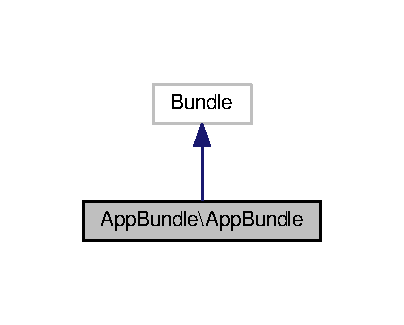
\includegraphics[width=194pt]{classAppBundle_1_1AppBundle__inherit__graph}
\end{center}
\end{figure}


Graphe de collaboration de App\+Bundle\textbackslash{}App\+Bundle\+:\nopagebreak
\begin{figure}[H]
\begin{center}
\leavevmode
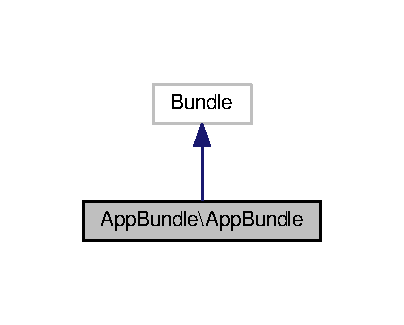
\includegraphics[width=194pt]{classAppBundle_1_1AppBundle__coll__graph}
\end{center}
\end{figure}


La documentation de cette classe a été générée à partir du fichier suivant \+:\begin{DoxyCompactItemize}
\item 
src/\+App\+Bundle/App\+Bundle.\+php\end{DoxyCompactItemize}

\hypertarget{classAppCache}{}\section{Référence de la classe App\+Cache}
\label{classAppCache}\index{App\+Cache@{App\+Cache}}


Graphe d\textquotesingle{}héritage de App\+Cache\+:\nopagebreak
\begin{figure}[H]
\begin{center}
\leavevmode
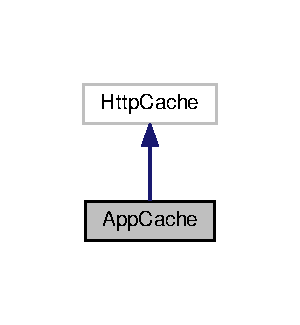
\includegraphics[width=144pt]{classAppCache__inherit__graph}
\end{center}
\end{figure}


Graphe de collaboration de App\+Cache\+:\nopagebreak
\begin{figure}[H]
\begin{center}
\leavevmode
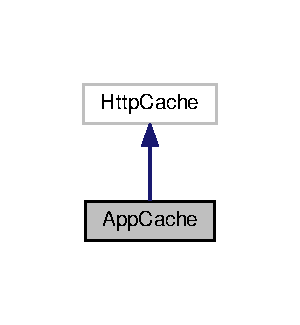
\includegraphics[width=144pt]{classAppCache__coll__graph}
\end{center}
\end{figure}


La documentation de cette classe a été générée à partir du fichier suivant \+:\begin{DoxyCompactItemize}
\item 
app/App\+Cache.\+php\end{DoxyCompactItemize}

\hypertarget{classAppKernel}{}\section{Référence de la classe App\+Kernel}
\label{classAppKernel}\index{App\+Kernel@{App\+Kernel}}


Graphe d\textquotesingle{}héritage de App\+Kernel\+:\nopagebreak
\begin{figure}[H]
\begin{center}
\leavevmode
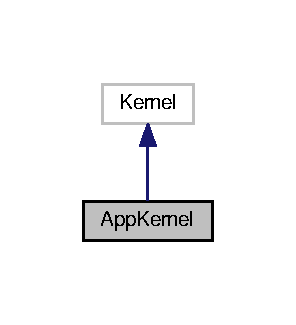
\includegraphics[width=142pt]{classAppKernel__inherit__graph}
\end{center}
\end{figure}


Graphe de collaboration de App\+Kernel\+:\nopagebreak
\begin{figure}[H]
\begin{center}
\leavevmode
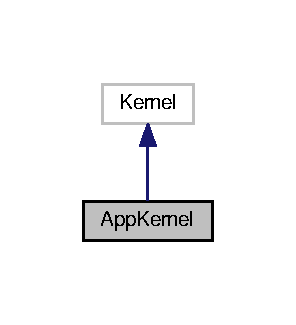
\includegraphics[width=142pt]{classAppKernel__coll__graph}
\end{center}
\end{figure}
\subsection*{Fonctions membres publiques}
\begin{DoxyCompactItemize}
\item 
\mbox{\Hypertarget{classAppKernel_a7b5d37c914be200c1350ec7139931761}\label{classAppKernel_a7b5d37c914be200c1350ec7139931761}} 
{\bfseries register\+Bundles} ()
\item 
\mbox{\Hypertarget{classAppKernel_a6e89dc2765c1eef6d90b59a630b47dce}\label{classAppKernel_a6e89dc2765c1eef6d90b59a630b47dce}} 
{\bfseries get\+Root\+Dir} ()
\item 
\mbox{\Hypertarget{classAppKernel_aa25ceee5054b99a4964b443964ead6f0}\label{classAppKernel_aa25ceee5054b99a4964b443964ead6f0}} 
{\bfseries get\+Cache\+Dir} ()
\item 
\mbox{\Hypertarget{classAppKernel_a6e3549c8ae2f237976c977dc21780f0c}\label{classAppKernel_a6e3549c8ae2f237976c977dc21780f0c}} 
{\bfseries get\+Log\+Dir} ()
\item 
\mbox{\Hypertarget{classAppKernel_a19fe2c7fcbfebedd149afd68f42475f3}\label{classAppKernel_a19fe2c7fcbfebedd149afd68f42475f3}} 
{\bfseries register\+Container\+Configuration} (Loader\+Interface \$loader)
\end{DoxyCompactItemize}


La documentation de cette classe a été générée à partir du fichier suivant \+:\begin{DoxyCompactItemize}
\item 
app/App\+Kernel.\+php\end{DoxyCompactItemize}

\hypertarget{classAppBundle_1_1Controller_1_1CommunityController}{}\section{Référence de la classe App\+Bundle\textbackslash{}Controller\textbackslash{}Community\+Controller}
\label{classAppBundle_1_1Controller_1_1CommunityController}\index{App\+Bundle\textbackslash{}\+Controller\textbackslash{}\+Community\+Controller@{App\+Bundle\textbackslash{}\+Controller\textbackslash{}\+Community\+Controller}}


Graphe d\textquotesingle{}héritage de App\+Bundle\textbackslash{}Controller\textbackslash{}Community\+Controller\+:\nopagebreak
\begin{figure}[H]
\begin{center}
\leavevmode
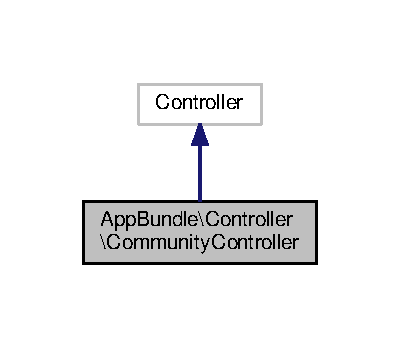
\includegraphics[width=192pt]{classAppBundle_1_1Controller_1_1CommunityController__inherit__graph}
\end{center}
\end{figure}


Graphe de collaboration de App\+Bundle\textbackslash{}Controller\textbackslash{}Community\+Controller\+:\nopagebreak
\begin{figure}[H]
\begin{center}
\leavevmode
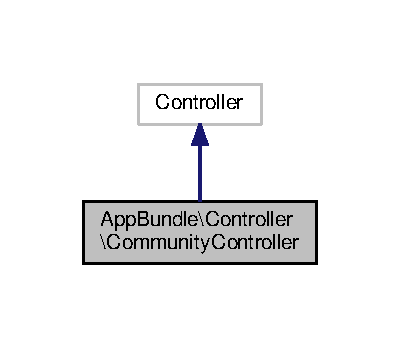
\includegraphics[width=192pt]{classAppBundle_1_1Controller_1_1CommunityController__coll__graph}
\end{center}
\end{figure}
\subsection*{Fonctions membres publiques}
\begin{DoxyCompactItemize}
\item 
\hyperlink{classAppBundle_1_1Controller_1_1CommunityController_a9a16d7753fcbdaa82cd3f56d5b117389}{profile\+Action} (\$username, Request \$request)
\item 
\hyperlink{classAppBundle_1_1Controller_1_1CommunityController_a254fe03f9c5d22aced8c6fd8bf8fd98d}{profile\+Edit} (Request \$request, string \$username)
\item 
\hyperlink{classAppBundle_1_1Controller_1_1CommunityController_af9281a620be8afbfebcef4910ede38fa}{add\+Friend} (Request \$request)
\item 
\hyperlink{classAppBundle_1_1Controller_1_1CommunityController_afe7246d7f115e157d6ab07a662fcbced}{remove\+Friend} (Request \$request)
\item 
\hyperlink{classAppBundle_1_1Controller_1_1CommunityController_aaec352ba9138f094ebeb67cc84f1c2f2}{accept\+Friend\+Request} (Request \$request)
\item 
\hyperlink{classAppBundle_1_1Controller_1_1CommunityController_a4db8318b023676b683c0aec7c5c260ff}{remove\+Friend\+Request} (Request \$request)
\item 
\hyperlink{classAppBundle_1_1Controller_1_1CommunityController_a7f26d8a801e9ab7b910e9bf6f76cacd6}{add\+Favorite\+Action} (Request \$request)
\item 
\hyperlink{classAppBundle_1_1Controller_1_1CommunityController_aabe67faadd72f242589b5459ce11d7ad}{remove\+Favorite\+Action} (Request \$request)
\item 
\hyperlink{classAppBundle_1_1Controller_1_1CommunityController_a0dda1cbb4b9bb323a51ff7c819f32290}{get\+Location\+Action} (Request \$request)
\item 
\hyperlink{classAppBundle_1_1Controller_1_1CommunityController_a0086746446df9fc76784d057babe7708}{join\+Event\+Action} (Request \$request)
\item 
\hyperlink{classAppBundle_1_1Controller_1_1CommunityController_a20e8b943a1cdc78683436cf32d17b6f1}{quit\+Event\+Action} (Request \$request)
\item 
\hyperlink{classAppBundle_1_1Controller_1_1CommunityController_a5d054da3bc5bdcbdaf4fe460ee12cb97}{update\+Cities\+Action} (Request \$request)
\end{DoxyCompactItemize}


\subsection{Documentation des fonctions membres}
\mbox{\Hypertarget{classAppBundle_1_1Controller_1_1CommunityController_aaec352ba9138f094ebeb67cc84f1c2f2}\label{classAppBundle_1_1Controller_1_1CommunityController_aaec352ba9138f094ebeb67cc84f1c2f2}} 
\index{App\+Bundle\+::\+Controller\+::\+Community\+Controller@{App\+Bundle\+::\+Controller\+::\+Community\+Controller}!accept\+Friend\+Request@{accept\+Friend\+Request}}
\index{accept\+Friend\+Request@{accept\+Friend\+Request}!App\+Bundle\+::\+Controller\+::\+Community\+Controller@{App\+Bundle\+::\+Controller\+::\+Community\+Controller}}
\subsubsection{\texorpdfstring{accept\+Friend\+Request()}{acceptFriendRequest()}}
{\footnotesize\ttfamily App\+Bundle\textbackslash{}\+Controller\textbackslash{}\+Community\+Controller\+::accept\+Friend\+Request (\begin{DoxyParamCaption}\item[{Request}]{\$request }\end{DoxyParamCaption})}

(\char`\"{}/community/accept-\/request\char`\"{}, name=\char`\"{}accept-\/request\char`\"{}, options=\{\char`\"{}expose\char`\"{} = true\}) 
\begin{DoxyParams}[1]{Paramètres}
Request & {\em \$request} & \\
\hline
\end{DoxyParams}
\begin{DoxyReturn}{Renvoie}
Response 
\end{DoxyReturn}
\mbox{\Hypertarget{classAppBundle_1_1Controller_1_1CommunityController_a7f26d8a801e9ab7b910e9bf6f76cacd6}\label{classAppBundle_1_1Controller_1_1CommunityController_a7f26d8a801e9ab7b910e9bf6f76cacd6}} 
\index{App\+Bundle\+::\+Controller\+::\+Community\+Controller@{App\+Bundle\+::\+Controller\+::\+Community\+Controller}!add\+Favorite\+Action@{add\+Favorite\+Action}}
\index{add\+Favorite\+Action@{add\+Favorite\+Action}!App\+Bundle\+::\+Controller\+::\+Community\+Controller@{App\+Bundle\+::\+Controller\+::\+Community\+Controller}}
\subsubsection{\texorpdfstring{add\+Favorite\+Action()}{addFavoriteAction()}}
{\footnotesize\ttfamily App\+Bundle\textbackslash{}\+Controller\textbackslash{}\+Community\+Controller\+::add\+Favorite\+Action (\begin{DoxyParamCaption}\item[{Request}]{\$request }\end{DoxyParamCaption})}

(\char`\"{}/community/add-\/favorite\char`\"{}, name=\char`\"{}add-\/favorite\char`\"{}, options=\{\char`\"{}expose\char`\"{} = true\}) 
\begin{DoxyParams}[1]{Paramètres}
Request & {\em \$request} & \\
\hline
\end{DoxyParams}
\begin{DoxyReturn}{Renvoie}
Response 
\end{DoxyReturn}
\mbox{\Hypertarget{classAppBundle_1_1Controller_1_1CommunityController_af9281a620be8afbfebcef4910ede38fa}\label{classAppBundle_1_1Controller_1_1CommunityController_af9281a620be8afbfebcef4910ede38fa}} 
\index{App\+Bundle\+::\+Controller\+::\+Community\+Controller@{App\+Bundle\+::\+Controller\+::\+Community\+Controller}!add\+Friend@{add\+Friend}}
\index{add\+Friend@{add\+Friend}!App\+Bundle\+::\+Controller\+::\+Community\+Controller@{App\+Bundle\+::\+Controller\+::\+Community\+Controller}}
\subsubsection{\texorpdfstring{add\+Friend()}{addFriend()}}
{\footnotesize\ttfamily App\+Bundle\textbackslash{}\+Controller\textbackslash{}\+Community\+Controller\+::add\+Friend (\begin{DoxyParamCaption}\item[{Request}]{\$request }\end{DoxyParamCaption})}

(\char`\"{}/community/add-\/friend\char`\"{}, name=\char`\"{}add-\/\+Friend\char`\"{}, options=\{\char`\"{}expose\char`\"{} = true\}) 
\begin{DoxyParams}[1]{Paramètres}
Request & {\em \$request} & \\
\hline
\end{DoxyParams}
\begin{DoxyReturn}{Renvoie}
Response 
\end{DoxyReturn}
\mbox{\Hypertarget{classAppBundle_1_1Controller_1_1CommunityController_a0dda1cbb4b9bb323a51ff7c819f32290}\label{classAppBundle_1_1Controller_1_1CommunityController_a0dda1cbb4b9bb323a51ff7c819f32290}} 
\index{App\+Bundle\+::\+Controller\+::\+Community\+Controller@{App\+Bundle\+::\+Controller\+::\+Community\+Controller}!get\+Location\+Action@{get\+Location\+Action}}
\index{get\+Location\+Action@{get\+Location\+Action}!App\+Bundle\+::\+Controller\+::\+Community\+Controller@{App\+Bundle\+::\+Controller\+::\+Community\+Controller}}
\subsubsection{\texorpdfstring{get\+Location\+Action()}{getLocationAction()}}
{\footnotesize\ttfamily App\+Bundle\textbackslash{}\+Controller\textbackslash{}\+Community\+Controller\+::get\+Location\+Action (\begin{DoxyParamCaption}\item[{Request}]{\$request }\end{DoxyParamCaption})}

(\char`\"{}/community/get-\/location\char`\"{}, name=\char`\"{}get-\/location\char`\"{}, options=\{\char`\"{}expose\char`\"{} = true\}) 
\begin{DoxyParams}[1]{Paramètres}
Request & {\em \$request} & \\
\hline
\end{DoxyParams}
\begin{DoxyReturn}{Renvoie}
Response 
\end{DoxyReturn}
\mbox{\Hypertarget{classAppBundle_1_1Controller_1_1CommunityController_a0086746446df9fc76784d057babe7708}\label{classAppBundle_1_1Controller_1_1CommunityController_a0086746446df9fc76784d057babe7708}} 
\index{App\+Bundle\+::\+Controller\+::\+Community\+Controller@{App\+Bundle\+::\+Controller\+::\+Community\+Controller}!join\+Event\+Action@{join\+Event\+Action}}
\index{join\+Event\+Action@{join\+Event\+Action}!App\+Bundle\+::\+Controller\+::\+Community\+Controller@{App\+Bundle\+::\+Controller\+::\+Community\+Controller}}
\subsubsection{\texorpdfstring{join\+Event\+Action()}{joinEventAction()}}
{\footnotesize\ttfamily App\+Bundle\textbackslash{}\+Controller\textbackslash{}\+Community\+Controller\+::join\+Event\+Action (\begin{DoxyParamCaption}\item[{Request}]{\$request }\end{DoxyParamCaption})}

(\char`\"{}/community/join-\/event\char`\"{}, name=\char`\"{}join-\/event\char`\"{}, options=\{\char`\"{}expose\char`\"{} = true\}) 
\begin{DoxyParams}[1]{Paramètres}
Request & {\em \$request} & \\
\hline
\end{DoxyParams}
\begin{DoxyReturn}{Renvoie}
Response 
\end{DoxyReturn}
\mbox{\Hypertarget{classAppBundle_1_1Controller_1_1CommunityController_a9a16d7753fcbdaa82cd3f56d5b117389}\label{classAppBundle_1_1Controller_1_1CommunityController_a9a16d7753fcbdaa82cd3f56d5b117389}} 
\index{App\+Bundle\+::\+Controller\+::\+Community\+Controller@{App\+Bundle\+::\+Controller\+::\+Community\+Controller}!profile\+Action@{profile\+Action}}
\index{profile\+Action@{profile\+Action}!App\+Bundle\+::\+Controller\+::\+Community\+Controller@{App\+Bundle\+::\+Controller\+::\+Community\+Controller}}
\subsubsection{\texorpdfstring{profile\+Action()}{profileAction()}}
{\footnotesize\ttfamily App\+Bundle\textbackslash{}\+Controller\textbackslash{}\+Community\+Controller\+::profile\+Action (\begin{DoxyParamCaption}\item[{}]{\$username,  }\item[{Request}]{\$request }\end{DoxyParamCaption})}

(\char`\"{}/profile/\{username\}\char`\"{}, name=\char`\"{}profile-\/index\char`\"{}) 
\begin{DoxyParams}[1]{Paramètres}
 & {\em \$username} & \\
\hline
Request & {\em \$request} & \\
\hline
\end{DoxyParams}
\begin{DoxyReturn}{Renvoie}
Response 
\end{DoxyReturn}
\mbox{\Hypertarget{classAppBundle_1_1Controller_1_1CommunityController_a254fe03f9c5d22aced8c6fd8bf8fd98d}\label{classAppBundle_1_1Controller_1_1CommunityController_a254fe03f9c5d22aced8c6fd8bf8fd98d}} 
\index{App\+Bundle\+::\+Controller\+::\+Community\+Controller@{App\+Bundle\+::\+Controller\+::\+Community\+Controller}!profile\+Edit@{profile\+Edit}}
\index{profile\+Edit@{profile\+Edit}!App\+Bundle\+::\+Controller\+::\+Community\+Controller@{App\+Bundle\+::\+Controller\+::\+Community\+Controller}}
\subsubsection{\texorpdfstring{profile\+Edit()}{profileEdit()}}
{\footnotesize\ttfamily App\+Bundle\textbackslash{}\+Controller\textbackslash{}\+Community\+Controller\+::profile\+Edit (\begin{DoxyParamCaption}\item[{Request}]{\$request,  }\item[{string}]{\$username }\end{DoxyParamCaption})}

(\char`\"{}/profile/\{username\}/edit\char`\"{}, name=\char`\"{}profile-\/edit\char`\"{}) 
\begin{DoxyParams}[1]{Paramètres}
Request & {\em \$request} & \\
\hline
string & {\em \$username} & \\
\hline
\end{DoxyParams}
\begin{DoxyReturn}{Renvoie}
Redirect\+Response$\vert$\+Response 
\end{DoxyReturn}
\mbox{\Hypertarget{classAppBundle_1_1Controller_1_1CommunityController_a20e8b943a1cdc78683436cf32d17b6f1}\label{classAppBundle_1_1Controller_1_1CommunityController_a20e8b943a1cdc78683436cf32d17b6f1}} 
\index{App\+Bundle\+::\+Controller\+::\+Community\+Controller@{App\+Bundle\+::\+Controller\+::\+Community\+Controller}!quit\+Event\+Action@{quit\+Event\+Action}}
\index{quit\+Event\+Action@{quit\+Event\+Action}!App\+Bundle\+::\+Controller\+::\+Community\+Controller@{App\+Bundle\+::\+Controller\+::\+Community\+Controller}}
\subsubsection{\texorpdfstring{quit\+Event\+Action()}{quitEventAction()}}
{\footnotesize\ttfamily App\+Bundle\textbackslash{}\+Controller\textbackslash{}\+Community\+Controller\+::quit\+Event\+Action (\begin{DoxyParamCaption}\item[{Request}]{\$request }\end{DoxyParamCaption})}

(\char`\"{}/community/quit-\/event\char`\"{}, name=\char`\"{}quit-\/event\char`\"{}, options=\{\char`\"{}expose\char`\"{} = true\}) 
\begin{DoxyParams}[1]{Paramètres}
Request & {\em \$request} & \\
\hline
\end{DoxyParams}
\begin{DoxyReturn}{Renvoie}
Response 
\end{DoxyReturn}
\mbox{\Hypertarget{classAppBundle_1_1Controller_1_1CommunityController_aabe67faadd72f242589b5459ce11d7ad}\label{classAppBundle_1_1Controller_1_1CommunityController_aabe67faadd72f242589b5459ce11d7ad}} 
\index{App\+Bundle\+::\+Controller\+::\+Community\+Controller@{App\+Bundle\+::\+Controller\+::\+Community\+Controller}!remove\+Favorite\+Action@{remove\+Favorite\+Action}}
\index{remove\+Favorite\+Action@{remove\+Favorite\+Action}!App\+Bundle\+::\+Controller\+::\+Community\+Controller@{App\+Bundle\+::\+Controller\+::\+Community\+Controller}}
\subsubsection{\texorpdfstring{remove\+Favorite\+Action()}{removeFavoriteAction()}}
{\footnotesize\ttfamily App\+Bundle\textbackslash{}\+Controller\textbackslash{}\+Community\+Controller\+::remove\+Favorite\+Action (\begin{DoxyParamCaption}\item[{Request}]{\$request }\end{DoxyParamCaption})}

(\char`\"{}/community/remove-\/favorite\char`\"{}, name=\char`\"{}remove-\/favorite\char`\"{}, options=\{\char`\"{}expose\char`\"{} = true\}) 
\begin{DoxyParams}[1]{Paramètres}
Request & {\em \$request} & \\
\hline
\end{DoxyParams}
\begin{DoxyReturn}{Renvoie}
Response 
\end{DoxyReturn}
\mbox{\Hypertarget{classAppBundle_1_1Controller_1_1CommunityController_afe7246d7f115e157d6ab07a662fcbced}\label{classAppBundle_1_1Controller_1_1CommunityController_afe7246d7f115e157d6ab07a662fcbced}} 
\index{App\+Bundle\+::\+Controller\+::\+Community\+Controller@{App\+Bundle\+::\+Controller\+::\+Community\+Controller}!remove\+Friend@{remove\+Friend}}
\index{remove\+Friend@{remove\+Friend}!App\+Bundle\+::\+Controller\+::\+Community\+Controller@{App\+Bundle\+::\+Controller\+::\+Community\+Controller}}
\subsubsection{\texorpdfstring{remove\+Friend()}{removeFriend()}}
{\footnotesize\ttfamily App\+Bundle\textbackslash{}\+Controller\textbackslash{}\+Community\+Controller\+::remove\+Friend (\begin{DoxyParamCaption}\item[{Request}]{\$request }\end{DoxyParamCaption})}

(\char`\"{}/community/remove-\/friend\char`\"{}, name=\char`\"{}remove-\/\+Friend\char`\"{}, options=\{\char`\"{}expose\char`\"{} = true\}) 
\begin{DoxyParams}[1]{Paramètres}
Request & {\em \$request} & \\
\hline
\end{DoxyParams}
\begin{DoxyReturn}{Renvoie}
Response 
\end{DoxyReturn}
\mbox{\Hypertarget{classAppBundle_1_1Controller_1_1CommunityController_a4db8318b023676b683c0aec7c5c260ff}\label{classAppBundle_1_1Controller_1_1CommunityController_a4db8318b023676b683c0aec7c5c260ff}} 
\index{App\+Bundle\+::\+Controller\+::\+Community\+Controller@{App\+Bundle\+::\+Controller\+::\+Community\+Controller}!remove\+Friend\+Request@{remove\+Friend\+Request}}
\index{remove\+Friend\+Request@{remove\+Friend\+Request}!App\+Bundle\+::\+Controller\+::\+Community\+Controller@{App\+Bundle\+::\+Controller\+::\+Community\+Controller}}
\subsubsection{\texorpdfstring{remove\+Friend\+Request()}{removeFriendRequest()}}
{\footnotesize\ttfamily App\+Bundle\textbackslash{}\+Controller\textbackslash{}\+Community\+Controller\+::remove\+Friend\+Request (\begin{DoxyParamCaption}\item[{Request}]{\$request }\end{DoxyParamCaption})}

(\char`\"{}/community/remove-\/request\char`\"{}, name=\char`\"{}remove-\/request\char`\"{}, options=\{\char`\"{}expose\char`\"{} = true\}) 
\begin{DoxyParams}[1]{Paramètres}
Request & {\em \$request} & \\
\hline
\end{DoxyParams}
\begin{DoxyReturn}{Renvoie}
Response 
\end{DoxyReturn}
\mbox{\Hypertarget{classAppBundle_1_1Controller_1_1CommunityController_a5d054da3bc5bdcbdaf4fe460ee12cb97}\label{classAppBundle_1_1Controller_1_1CommunityController_a5d054da3bc5bdcbdaf4fe460ee12cb97}} 
\index{App\+Bundle\+::\+Controller\+::\+Community\+Controller@{App\+Bundle\+::\+Controller\+::\+Community\+Controller}!update\+Cities\+Action@{update\+Cities\+Action}}
\index{update\+Cities\+Action@{update\+Cities\+Action}!App\+Bundle\+::\+Controller\+::\+Community\+Controller@{App\+Bundle\+::\+Controller\+::\+Community\+Controller}}
\subsubsection{\texorpdfstring{update\+Cities\+Action()}{updateCitiesAction()}}
{\footnotesize\ttfamily App\+Bundle\textbackslash{}\+Controller\textbackslash{}\+Community\+Controller\+::update\+Cities\+Action (\begin{DoxyParamCaption}\item[{Request}]{\$request }\end{DoxyParamCaption})}

(\char`\"{}/community/update-\/cities\char`\"{}, name=\char`\"{}update-\/stats-\/cities\char`\"{}, options=\{\char`\"{}expose\char`\"{} = true\}) 
\begin{DoxyParams}[1]{Paramètres}
Request & {\em \$request} & \\
\hline
\end{DoxyParams}
\begin{DoxyReturn}{Renvoie}
Response 
\end{DoxyReturn}


La documentation de cette classe a été générée à partir du fichier suivant \+:\begin{DoxyCompactItemize}
\item 
src/\+App\+Bundle/\+Controller/Community\+Controller.\+php\end{DoxyCompactItemize}

\hypertarget{classAppBundle_1_1Controller_1_1DefaultController}{}\section{Référence de la classe App\+Bundle\textbackslash{}Controller\textbackslash{}Default\+Controller}
\label{classAppBundle_1_1Controller_1_1DefaultController}\index{App\+Bundle\textbackslash{}\+Controller\textbackslash{}\+Default\+Controller@{App\+Bundle\textbackslash{}\+Controller\textbackslash{}\+Default\+Controller}}


Graphe d\textquotesingle{}héritage de App\+Bundle\textbackslash{}Controller\textbackslash{}Default\+Controller\+:\nopagebreak
\begin{figure}[H]
\begin{center}
\leavevmode
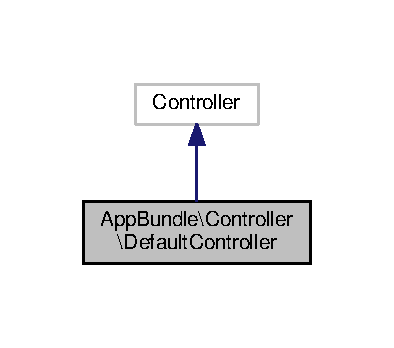
\includegraphics[width=189pt]{classAppBundle_1_1Controller_1_1DefaultController__inherit__graph}
\end{center}
\end{figure}


Graphe de collaboration de App\+Bundle\textbackslash{}Controller\textbackslash{}Default\+Controller\+:\nopagebreak
\begin{figure}[H]
\begin{center}
\leavevmode
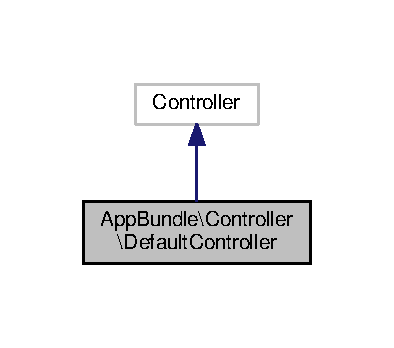
\includegraphics[width=189pt]{classAppBundle_1_1Controller_1_1DefaultController__coll__graph}
\end{center}
\end{figure}
\subsection*{Fonctions membres publiques}
\begin{DoxyCompactItemize}
\item 
\hyperlink{classAppBundle_1_1Controller_1_1DefaultController_a8b0b26b1f8263360cfda801eef12e876}{index\+Action} (Request \$request)
\item 
\hyperlink{classAppBundle_1_1Controller_1_1DefaultController_a0e05a88ad81bdd7d285ed7f5e18e4db3}{app\+Coordinates\+Action} (\$lat, \$lon, Request \$request)
\item 
\hyperlink{classAppBundle_1_1Controller_1_1DefaultController_ad7e4ef81807736ad3c44c7b34b43410f}{app\+Action} (Request \$request)
\end{DoxyCompactItemize}


\subsection{Documentation des fonctions membres}
\mbox{\Hypertarget{classAppBundle_1_1Controller_1_1DefaultController_ad7e4ef81807736ad3c44c7b34b43410f}\label{classAppBundle_1_1Controller_1_1DefaultController_ad7e4ef81807736ad3c44c7b34b43410f}} 
\index{App\+Bundle\+::\+Controller\+::\+Default\+Controller@{App\+Bundle\+::\+Controller\+::\+Default\+Controller}!app\+Action@{app\+Action}}
\index{app\+Action@{app\+Action}!App\+Bundle\+::\+Controller\+::\+Default\+Controller@{App\+Bundle\+::\+Controller\+::\+Default\+Controller}}
\subsubsection{\texorpdfstring{app\+Action()}{appAction()}}
{\footnotesize\ttfamily App\+Bundle\textbackslash{}\+Controller\textbackslash{}\+Default\+Controller\+::app\+Action (\begin{DoxyParamCaption}\item[{Request}]{\$request }\end{DoxyParamCaption})}

(\char`\"{}/app\char`\"{}, name=\char`\"{}app\char`\"{}) \mbox{\Hypertarget{classAppBundle_1_1Controller_1_1DefaultController_a0e05a88ad81bdd7d285ed7f5e18e4db3}\label{classAppBundle_1_1Controller_1_1DefaultController_a0e05a88ad81bdd7d285ed7f5e18e4db3}} 
\index{App\+Bundle\+::\+Controller\+::\+Default\+Controller@{App\+Bundle\+::\+Controller\+::\+Default\+Controller}!app\+Coordinates\+Action@{app\+Coordinates\+Action}}
\index{app\+Coordinates\+Action@{app\+Coordinates\+Action}!App\+Bundle\+::\+Controller\+::\+Default\+Controller@{App\+Bundle\+::\+Controller\+::\+Default\+Controller}}
\subsubsection{\texorpdfstring{app\+Coordinates\+Action()}{appCoordinatesAction()}}
{\footnotesize\ttfamily App\+Bundle\textbackslash{}\+Controller\textbackslash{}\+Default\+Controller\+::app\+Coordinates\+Action (\begin{DoxyParamCaption}\item[{}]{\$lat,  }\item[{}]{\$lon,  }\item[{Request}]{\$request }\end{DoxyParamCaption})}

(\char`\"{}/app/coordinates/\{lat\}/\{lon\}\char`\"{}, name=\char`\"{}app-\/coordinates\char`\"{}) 
\begin{DoxyParams}[1]{Paramètres}
Request & {\em \$request} & \\
\hline
 & {\em \$lat} & \\
\hline
 & {\em \$lon} & \\
\hline
\end{DoxyParams}
\begin{DoxyReturn}{Renvoie}

\end{DoxyReturn}
\mbox{\Hypertarget{classAppBundle_1_1Controller_1_1DefaultController_a8b0b26b1f8263360cfda801eef12e876}\label{classAppBundle_1_1Controller_1_1DefaultController_a8b0b26b1f8263360cfda801eef12e876}} 
\index{App\+Bundle\+::\+Controller\+::\+Default\+Controller@{App\+Bundle\+::\+Controller\+::\+Default\+Controller}!index\+Action@{index\+Action}}
\index{index\+Action@{index\+Action}!App\+Bundle\+::\+Controller\+::\+Default\+Controller@{App\+Bundle\+::\+Controller\+::\+Default\+Controller}}
\subsubsection{\texorpdfstring{index\+Action()}{indexAction()}}
{\footnotesize\ttfamily App\+Bundle\textbackslash{}\+Controller\textbackslash{}\+Default\+Controller\+::index\+Action (\begin{DoxyParamCaption}\item[{Request}]{\$request }\end{DoxyParamCaption})}

(\char`\"{}/\char`\"{}, name=\char`\"{}homepage\char`\"{}) 

La documentation de cette classe a été générée à partir du fichier suivant \+:\begin{DoxyCompactItemize}
\item 
src/\+App\+Bundle/\+Controller/Default\+Controller.\+php\end{DoxyCompactItemize}

\hypertarget{classTests_1_1AppBundle_1_1Controller_1_1DefaultControllerTest}{}\section{Référence de la classe Tests\textbackslash{}App\+Bundle\textbackslash{}Controller\textbackslash{}Default\+Controller\+Test}
\label{classTests_1_1AppBundle_1_1Controller_1_1DefaultControllerTest}\index{Tests\textbackslash{}\+App\+Bundle\textbackslash{}\+Controller\textbackslash{}\+Default\+Controller\+Test@{Tests\textbackslash{}\+App\+Bundle\textbackslash{}\+Controller\textbackslash{}\+Default\+Controller\+Test}}


Graphe d\textquotesingle{}héritage de Tests\textbackslash{}App\+Bundle\textbackslash{}Controller\textbackslash{}Default\+Controller\+Test\+:\nopagebreak
\begin{figure}[H]
\begin{center}
\leavevmode
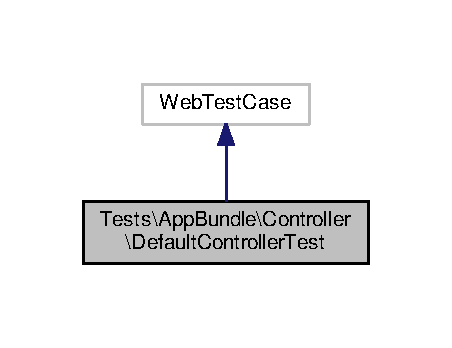
\includegraphics[width=217pt]{classTests_1_1AppBundle_1_1Controller_1_1DefaultControllerTest__inherit__graph}
\end{center}
\end{figure}


Graphe de collaboration de Tests\textbackslash{}App\+Bundle\textbackslash{}Controller\textbackslash{}Default\+Controller\+Test\+:\nopagebreak
\begin{figure}[H]
\begin{center}
\leavevmode
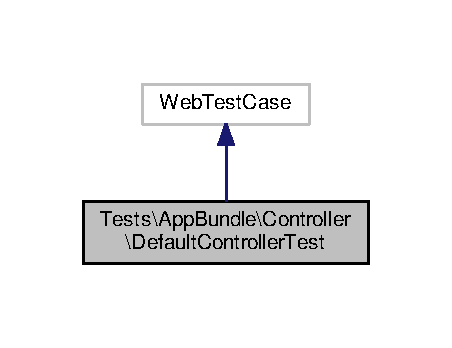
\includegraphics[width=217pt]{classTests_1_1AppBundle_1_1Controller_1_1DefaultControllerTest__coll__graph}
\end{center}
\end{figure}
\subsection*{Fonctions membres publiques}
\begin{DoxyCompactItemize}
\item 
\mbox{\Hypertarget{classTests_1_1AppBundle_1_1Controller_1_1DefaultControllerTest_af5162a9f3808a733b782c281bf3d5bb5}\label{classTests_1_1AppBundle_1_1Controller_1_1DefaultControllerTest_af5162a9f3808a733b782c281bf3d5bb5}} 
{\bfseries test\+App} ()
\item 
\mbox{\Hypertarget{classTests_1_1AppBundle_1_1Controller_1_1DefaultControllerTest_ac9ef62ffe6807485a78118db1d60bb11}\label{classTests_1_1AppBundle_1_1Controller_1_1DefaultControllerTest_ac9ef62ffe6807485a78118db1d60bb11}} 
{\bfseries test\+App\+Coordinates} ()
\end{DoxyCompactItemize}


La documentation de cette classe a été générée à partir du fichier suivant \+:\begin{DoxyCompactItemize}
\item 
tests/\+App\+Bundle/\+Controller/Default\+Controller\+Test.\+php\end{DoxyCompactItemize}

\hypertarget{classAppBundle_1_1Entity_1_1Event}{}\section{Référence de la classe App\+Bundle\textbackslash{}Entity\textbackslash{}Event}
\label{classAppBundle_1_1Entity_1_1Event}\index{App\+Bundle\textbackslash{}\+Entity\textbackslash{}\+Event@{App\+Bundle\textbackslash{}\+Entity\textbackslash{}\+Event}}
\subsection*{Fonctions membres publiques}
\begin{DoxyCompactItemize}
\item 
\hyperlink{classAppBundle_1_1Entity_1_1Event_a6114bdcf3b095f77e8149d7b996c4d6d}{get\+Id} ()
\item 
\hyperlink{classAppBundle_1_1Entity_1_1Event_a834c71ca866cd9a1e88e5fcd105ef187}{set\+Name} (\$name)
\item 
\hyperlink{classAppBundle_1_1Entity_1_1Event_a342d43c67caedb66f9a0f87a0edf5e11}{get\+Name} ()
\item 
\hyperlink{classAppBundle_1_1Entity_1_1Event_ad9c16e367f4296df5b6dac59e1907c8c}{set\+Author} (\$author)
\item 
\hyperlink{classAppBundle_1_1Entity_1_1Event_a5a717cc787d1c40bdcb32ebf0c31b4c4}{get\+Author} ()
\item 
\hyperlink{classAppBundle_1_1Entity_1_1Event_a3d39550bcf4a114ebac3a021745d281f}{set\+Nb\+Participants} (\$nb\+Participants)
\item 
\hyperlink{classAppBundle_1_1Entity_1_1Event_a127aed01a9e943cdce793bf28a62032c}{get\+Nb\+Participants} ()
\item 
\hyperlink{classAppBundle_1_1Entity_1_1Event_a2104abbe1e799f1d01fa880a556c4b57}{set\+Participants} (\$participants)
\item 
\hyperlink{classAppBundle_1_1Entity_1_1Event_ad13574598ee9b60c47f5b3c7b4215d51}{get\+Participants} ()
\item 
\hyperlink{classAppBundle_1_1Entity_1_1Event_ab97fe1479bede8949391c7ade9112406}{set\+Description} (\$description)
\item 
\hyperlink{classAppBundle_1_1Entity_1_1Event_acfad608d5e348b26bc8b6646483d35b8}{get\+Description} ()
\item 
\hyperlink{classAppBundle_1_1Entity_1_1Event_ad738c33b2824cc1130b06c5bc7ace4d9}{\+\_\+\+\_\+construct} ()
\item 
\hyperlink{classAppBundle_1_1Entity_1_1Event_abc3d3ec1eb7e6d40ea11690e2321bfdc}{add\+Participant} (\textbackslash{}\hyperlink{classAppBundle_1_1Entity_1_1User}{App\+Bundle\textbackslash{}\+Entity\textbackslash{}\+User} \$participant)
\item 
\hyperlink{classAppBundle_1_1Entity_1_1Event_a86efd6b253de3449f7b1c4bec18ec6f5}{remove\+Participant} (\textbackslash{}\hyperlink{classAppBundle_1_1Entity_1_1User}{App\+Bundle\textbackslash{}\+Entity\textbackslash{}\+User} \$participant)
\item 
\hyperlink{classAppBundle_1_1Entity_1_1Event_a20b1f3bfc2c142e2b807384631101d06}{set\+Creation\+Date} (\$creation\+Date)
\item 
\hyperlink{classAppBundle_1_1Entity_1_1Event_a05d1bcc8c3f23ff96a5142b24ca2ea4e}{get\+Creation\+Date} ()
\item 
\hyperlink{classAppBundle_1_1Entity_1_1Event_ac0c53f2704cbff828187476552eab6a5}{set\+Trip\+Date} (\$trip\+Date)
\item 
\hyperlink{classAppBundle_1_1Entity_1_1Event_af2da1b9ca4e516fb74fa249a81400df7}{get\+Trip\+Date} ()
\item 
\hyperlink{classAppBundle_1_1Entity_1_1Event_a2b787c614b9f5e7f8908a33cb3f1c6fc}{set\+Start\+Point} (\textbackslash{}\hyperlink{classAppBundle_1_1Entity_1_1Location}{App\+Bundle\textbackslash{}\+Entity\textbackslash{}\+Location} \$start\+Point)
\item 
\hyperlink{classAppBundle_1_1Entity_1_1Event_a530176fae73c30a523eb27824e2be5ce}{get\+Start\+Point} ()
\item 
\hyperlink{classAppBundle_1_1Entity_1_1Event_aaa67dc26030fe5c273575c5c093aeb4b}{add\+Comment} (\textbackslash{}\hyperlink{classAppBundle_1_1Entity_1_1EventComment}{App\+Bundle\textbackslash{}\+Entity\textbackslash{}\+Event\+Comment} \$comment)
\item 
\hyperlink{classAppBundle_1_1Entity_1_1Event_ae18b32a77fca5c2ec3f7e71aedb8296f}{remove\+Comment} (\textbackslash{}\hyperlink{classAppBundle_1_1Entity_1_1EventComment}{App\+Bundle\textbackslash{}\+Entity\textbackslash{}\+Event\+Comment} \$comment)
\item 
\hyperlink{classAppBundle_1_1Entity_1_1Event_a00ba9c0f8c01d2a2a7c1a2d0f66d29de}{get\+Comments} ()
\end{DoxyCompactItemize}


\subsection{Description détaillée}
\hyperlink{classAppBundle_1_1Entity_1_1Event}{Event}

(name=\char`\"{}event\char`\"{}) (repository\+Class=\char`\"{}\+App\+Bundle\textbackslash{}\+Repository\textbackslash{}\+Event\+Repository\char`\"{}) 

\subsection{Documentation des constructeurs et destructeur}
\mbox{\Hypertarget{classAppBundle_1_1Entity_1_1Event_ad738c33b2824cc1130b06c5bc7ace4d9}\label{classAppBundle_1_1Entity_1_1Event_ad738c33b2824cc1130b06c5bc7ace4d9}} 
\index{App\+Bundle\+::\+Entity\+::\+Event@{App\+Bundle\+::\+Entity\+::\+Event}!\+\_\+\+\_\+construct@{\+\_\+\+\_\+construct}}
\index{\+\_\+\+\_\+construct@{\+\_\+\+\_\+construct}!App\+Bundle\+::\+Entity\+::\+Event@{App\+Bundle\+::\+Entity\+::\+Event}}
\subsubsection{\texorpdfstring{\+\_\+\+\_\+construct()}{\_\_construct()}}
{\footnotesize\ttfamily App\+Bundle\textbackslash{}\+Entity\textbackslash{}\+Event\+::\+\_\+\+\_\+construct (\begin{DoxyParamCaption}{ }\end{DoxyParamCaption})}

Constructor 

\subsection{Documentation des fonctions membres}
\mbox{\Hypertarget{classAppBundle_1_1Entity_1_1Event_aaa67dc26030fe5c273575c5c093aeb4b}\label{classAppBundle_1_1Entity_1_1Event_aaa67dc26030fe5c273575c5c093aeb4b}} 
\index{App\+Bundle\+::\+Entity\+::\+Event@{App\+Bundle\+::\+Entity\+::\+Event}!add\+Comment@{add\+Comment}}
\index{add\+Comment@{add\+Comment}!App\+Bundle\+::\+Entity\+::\+Event@{App\+Bundle\+::\+Entity\+::\+Event}}
\subsubsection{\texorpdfstring{add\+Comment()}{addComment()}}
{\footnotesize\ttfamily App\+Bundle\textbackslash{}\+Entity\textbackslash{}\+Event\+::add\+Comment (\begin{DoxyParamCaption}\item[{\textbackslash{}\hyperlink{classAppBundle_1_1Entity_1_1EventComment}{App\+Bundle\textbackslash{}\+Entity\textbackslash{}\+Event\+Comment}}]{\$comment }\end{DoxyParamCaption})}

Add comment


\begin{DoxyParams}[1]{Paramètres}
\textbackslash{}\+App\+Bundle\textbackslash{}\+Entity\textbackslash{}\+Event\+Comment & {\em \$comment} & \\
\hline
\end{DoxyParams}
\begin{DoxyReturn}{Renvoie}
\hyperlink{classAppBundle_1_1Entity_1_1Event}{Event} 
\end{DoxyReturn}
\mbox{\Hypertarget{classAppBundle_1_1Entity_1_1Event_abc3d3ec1eb7e6d40ea11690e2321bfdc}\label{classAppBundle_1_1Entity_1_1Event_abc3d3ec1eb7e6d40ea11690e2321bfdc}} 
\index{App\+Bundle\+::\+Entity\+::\+Event@{App\+Bundle\+::\+Entity\+::\+Event}!add\+Participant@{add\+Participant}}
\index{add\+Participant@{add\+Participant}!App\+Bundle\+::\+Entity\+::\+Event@{App\+Bundle\+::\+Entity\+::\+Event}}
\subsubsection{\texorpdfstring{add\+Participant()}{addParticipant()}}
{\footnotesize\ttfamily App\+Bundle\textbackslash{}\+Entity\textbackslash{}\+Event\+::add\+Participant (\begin{DoxyParamCaption}\item[{\textbackslash{}\hyperlink{classAppBundle_1_1Entity_1_1User}{App\+Bundle\textbackslash{}\+Entity\textbackslash{}\+User}}]{\$participant }\end{DoxyParamCaption})}

Add participant


\begin{DoxyParams}[1]{Paramètres}
\textbackslash{}\+App\+Bundle\textbackslash{}\+Entity\textbackslash{}\+User & {\em \$participant} & \\
\hline
\end{DoxyParams}
\begin{DoxyReturn}{Renvoie}
\hyperlink{classAppBundle_1_1Entity_1_1Event}{Event} 
\end{DoxyReturn}
\mbox{\Hypertarget{classAppBundle_1_1Entity_1_1Event_a5a717cc787d1c40bdcb32ebf0c31b4c4}\label{classAppBundle_1_1Entity_1_1Event_a5a717cc787d1c40bdcb32ebf0c31b4c4}} 
\index{App\+Bundle\+::\+Entity\+::\+Event@{App\+Bundle\+::\+Entity\+::\+Event}!get\+Author@{get\+Author}}
\index{get\+Author@{get\+Author}!App\+Bundle\+::\+Entity\+::\+Event@{App\+Bundle\+::\+Entity\+::\+Event}}
\subsubsection{\texorpdfstring{get\+Author()}{getAuthor()}}
{\footnotesize\ttfamily App\+Bundle\textbackslash{}\+Entity\textbackslash{}\+Event\+::get\+Author (\begin{DoxyParamCaption}{ }\end{DoxyParamCaption})}

Get author

\begin{DoxyReturn}{Renvoie}
string 
\end{DoxyReturn}
\mbox{\Hypertarget{classAppBundle_1_1Entity_1_1Event_a00ba9c0f8c01d2a2a7c1a2d0f66d29de}\label{classAppBundle_1_1Entity_1_1Event_a00ba9c0f8c01d2a2a7c1a2d0f66d29de}} 
\index{App\+Bundle\+::\+Entity\+::\+Event@{App\+Bundle\+::\+Entity\+::\+Event}!get\+Comments@{get\+Comments}}
\index{get\+Comments@{get\+Comments}!App\+Bundle\+::\+Entity\+::\+Event@{App\+Bundle\+::\+Entity\+::\+Event}}
\subsubsection{\texorpdfstring{get\+Comments()}{getComments()}}
{\footnotesize\ttfamily App\+Bundle\textbackslash{}\+Entity\textbackslash{}\+Event\+::get\+Comments (\begin{DoxyParamCaption}{ }\end{DoxyParamCaption})}

Get comments

\begin{DoxyReturn}{Renvoie}

\end{DoxyReturn}
\mbox{\Hypertarget{classAppBundle_1_1Entity_1_1Event_a05d1bcc8c3f23ff96a5142b24ca2ea4e}\label{classAppBundle_1_1Entity_1_1Event_a05d1bcc8c3f23ff96a5142b24ca2ea4e}} 
\index{App\+Bundle\+::\+Entity\+::\+Event@{App\+Bundle\+::\+Entity\+::\+Event}!get\+Creation\+Date@{get\+Creation\+Date}}
\index{get\+Creation\+Date@{get\+Creation\+Date}!App\+Bundle\+::\+Entity\+::\+Event@{App\+Bundle\+::\+Entity\+::\+Event}}
\subsubsection{\texorpdfstring{get\+Creation\+Date()}{getCreationDate()}}
{\footnotesize\ttfamily App\+Bundle\textbackslash{}\+Entity\textbackslash{}\+Event\+::get\+Creation\+Date (\begin{DoxyParamCaption}{ }\end{DoxyParamCaption})}

Get creation\+Date

\begin{DoxyReturn}{Renvoie}

\end{DoxyReturn}
\mbox{\Hypertarget{classAppBundle_1_1Entity_1_1Event_acfad608d5e348b26bc8b6646483d35b8}\label{classAppBundle_1_1Entity_1_1Event_acfad608d5e348b26bc8b6646483d35b8}} 
\index{App\+Bundle\+::\+Entity\+::\+Event@{App\+Bundle\+::\+Entity\+::\+Event}!get\+Description@{get\+Description}}
\index{get\+Description@{get\+Description}!App\+Bundle\+::\+Entity\+::\+Event@{App\+Bundle\+::\+Entity\+::\+Event}}
\subsubsection{\texorpdfstring{get\+Description()}{getDescription()}}
{\footnotesize\ttfamily App\+Bundle\textbackslash{}\+Entity\textbackslash{}\+Event\+::get\+Description (\begin{DoxyParamCaption}{ }\end{DoxyParamCaption})}

Get description

\begin{DoxyReturn}{Renvoie}
string 
\end{DoxyReturn}
\mbox{\Hypertarget{classAppBundle_1_1Entity_1_1Event_a6114bdcf3b095f77e8149d7b996c4d6d}\label{classAppBundle_1_1Entity_1_1Event_a6114bdcf3b095f77e8149d7b996c4d6d}} 
\index{App\+Bundle\+::\+Entity\+::\+Event@{App\+Bundle\+::\+Entity\+::\+Event}!get\+Id@{get\+Id}}
\index{get\+Id@{get\+Id}!App\+Bundle\+::\+Entity\+::\+Event@{App\+Bundle\+::\+Entity\+::\+Event}}
\subsubsection{\texorpdfstring{get\+Id()}{getId()}}
{\footnotesize\ttfamily App\+Bundle\textbackslash{}\+Entity\textbackslash{}\+Event\+::get\+Id (\begin{DoxyParamCaption}{ }\end{DoxyParamCaption})}

Get id

\begin{DoxyReturn}{Renvoie}
int 
\end{DoxyReturn}
\mbox{\Hypertarget{classAppBundle_1_1Entity_1_1Event_a342d43c67caedb66f9a0f87a0edf5e11}\label{classAppBundle_1_1Entity_1_1Event_a342d43c67caedb66f9a0f87a0edf5e11}} 
\index{App\+Bundle\+::\+Entity\+::\+Event@{App\+Bundle\+::\+Entity\+::\+Event}!get\+Name@{get\+Name}}
\index{get\+Name@{get\+Name}!App\+Bundle\+::\+Entity\+::\+Event@{App\+Bundle\+::\+Entity\+::\+Event}}
\subsubsection{\texorpdfstring{get\+Name()}{getName()}}
{\footnotesize\ttfamily App\+Bundle\textbackslash{}\+Entity\textbackslash{}\+Event\+::get\+Name (\begin{DoxyParamCaption}{ }\end{DoxyParamCaption})}

Get name

\begin{DoxyReturn}{Renvoie}
string 
\end{DoxyReturn}
\mbox{\Hypertarget{classAppBundle_1_1Entity_1_1Event_a127aed01a9e943cdce793bf28a62032c}\label{classAppBundle_1_1Entity_1_1Event_a127aed01a9e943cdce793bf28a62032c}} 
\index{App\+Bundle\+::\+Entity\+::\+Event@{App\+Bundle\+::\+Entity\+::\+Event}!get\+Nb\+Participants@{get\+Nb\+Participants}}
\index{get\+Nb\+Participants@{get\+Nb\+Participants}!App\+Bundle\+::\+Entity\+::\+Event@{App\+Bundle\+::\+Entity\+::\+Event}}
\subsubsection{\texorpdfstring{get\+Nb\+Participants()}{getNbParticipants()}}
{\footnotesize\ttfamily App\+Bundle\textbackslash{}\+Entity\textbackslash{}\+Event\+::get\+Nb\+Participants (\begin{DoxyParamCaption}{ }\end{DoxyParamCaption})}

Get nb\+Participants

\begin{DoxyReturn}{Renvoie}
int 
\end{DoxyReturn}
\mbox{\Hypertarget{classAppBundle_1_1Entity_1_1Event_ad13574598ee9b60c47f5b3c7b4215d51}\label{classAppBundle_1_1Entity_1_1Event_ad13574598ee9b60c47f5b3c7b4215d51}} 
\index{App\+Bundle\+::\+Entity\+::\+Event@{App\+Bundle\+::\+Entity\+::\+Event}!get\+Participants@{get\+Participants}}
\index{get\+Participants@{get\+Participants}!App\+Bundle\+::\+Entity\+::\+Event@{App\+Bundle\+::\+Entity\+::\+Event}}
\subsubsection{\texorpdfstring{get\+Participants()}{getParticipants()}}
{\footnotesize\ttfamily App\+Bundle\textbackslash{}\+Entity\textbackslash{}\+Event\+::get\+Participants (\begin{DoxyParamCaption}{ }\end{DoxyParamCaption})}

Get participants

\begin{DoxyReturn}{Renvoie}
string 
\end{DoxyReturn}
\mbox{\Hypertarget{classAppBundle_1_1Entity_1_1Event_a530176fae73c30a523eb27824e2be5ce}\label{classAppBundle_1_1Entity_1_1Event_a530176fae73c30a523eb27824e2be5ce}} 
\index{App\+Bundle\+::\+Entity\+::\+Event@{App\+Bundle\+::\+Entity\+::\+Event}!get\+Start\+Point@{get\+Start\+Point}}
\index{get\+Start\+Point@{get\+Start\+Point}!App\+Bundle\+::\+Entity\+::\+Event@{App\+Bundle\+::\+Entity\+::\+Event}}
\subsubsection{\texorpdfstring{get\+Start\+Point()}{getStartPoint()}}
{\footnotesize\ttfamily App\+Bundle\textbackslash{}\+Entity\textbackslash{}\+Event\+::get\+Start\+Point (\begin{DoxyParamCaption}{ }\end{DoxyParamCaption})}

Get start\+Point

\begin{DoxyReturn}{Renvoie}

\end{DoxyReturn}
\mbox{\Hypertarget{classAppBundle_1_1Entity_1_1Event_af2da1b9ca4e516fb74fa249a81400df7}\label{classAppBundle_1_1Entity_1_1Event_af2da1b9ca4e516fb74fa249a81400df7}} 
\index{App\+Bundle\+::\+Entity\+::\+Event@{App\+Bundle\+::\+Entity\+::\+Event}!get\+Trip\+Date@{get\+Trip\+Date}}
\index{get\+Trip\+Date@{get\+Trip\+Date}!App\+Bundle\+::\+Entity\+::\+Event@{App\+Bundle\+::\+Entity\+::\+Event}}
\subsubsection{\texorpdfstring{get\+Trip\+Date()}{getTripDate()}}
{\footnotesize\ttfamily App\+Bundle\textbackslash{}\+Entity\textbackslash{}\+Event\+::get\+Trip\+Date (\begin{DoxyParamCaption}{ }\end{DoxyParamCaption})}

Get trip\+Date

\begin{DoxyReturn}{Renvoie}

\end{DoxyReturn}
\mbox{\Hypertarget{classAppBundle_1_1Entity_1_1Event_ae18b32a77fca5c2ec3f7e71aedb8296f}\label{classAppBundle_1_1Entity_1_1Event_ae18b32a77fca5c2ec3f7e71aedb8296f}} 
\index{App\+Bundle\+::\+Entity\+::\+Event@{App\+Bundle\+::\+Entity\+::\+Event}!remove\+Comment@{remove\+Comment}}
\index{remove\+Comment@{remove\+Comment}!App\+Bundle\+::\+Entity\+::\+Event@{App\+Bundle\+::\+Entity\+::\+Event}}
\subsubsection{\texorpdfstring{remove\+Comment()}{removeComment()}}
{\footnotesize\ttfamily App\+Bundle\textbackslash{}\+Entity\textbackslash{}\+Event\+::remove\+Comment (\begin{DoxyParamCaption}\item[{\textbackslash{}\hyperlink{classAppBundle_1_1Entity_1_1EventComment}{App\+Bundle\textbackslash{}\+Entity\textbackslash{}\+Event\+Comment}}]{\$comment }\end{DoxyParamCaption})}

Remove comment


\begin{DoxyParams}[1]{Paramètres}
\textbackslash{}\+App\+Bundle\textbackslash{}\+Entity\textbackslash{}\+Event\+Comment & {\em \$comment} & \\
\hline
\end{DoxyParams}
\mbox{\Hypertarget{classAppBundle_1_1Entity_1_1Event_a86efd6b253de3449f7b1c4bec18ec6f5}\label{classAppBundle_1_1Entity_1_1Event_a86efd6b253de3449f7b1c4bec18ec6f5}} 
\index{App\+Bundle\+::\+Entity\+::\+Event@{App\+Bundle\+::\+Entity\+::\+Event}!remove\+Participant@{remove\+Participant}}
\index{remove\+Participant@{remove\+Participant}!App\+Bundle\+::\+Entity\+::\+Event@{App\+Bundle\+::\+Entity\+::\+Event}}
\subsubsection{\texorpdfstring{remove\+Participant()}{removeParticipant()}}
{\footnotesize\ttfamily App\+Bundle\textbackslash{}\+Entity\textbackslash{}\+Event\+::remove\+Participant (\begin{DoxyParamCaption}\item[{\textbackslash{}\hyperlink{classAppBundle_1_1Entity_1_1User}{App\+Bundle\textbackslash{}\+Entity\textbackslash{}\+User}}]{\$participant }\end{DoxyParamCaption})}

Remove participant


\begin{DoxyParams}[1]{Paramètres}
\textbackslash{}\+App\+Bundle\textbackslash{}\+Entity\textbackslash{}\+User & {\em \$participant} & \\
\hline
\end{DoxyParams}
\mbox{\Hypertarget{classAppBundle_1_1Entity_1_1Event_ad9c16e367f4296df5b6dac59e1907c8c}\label{classAppBundle_1_1Entity_1_1Event_ad9c16e367f4296df5b6dac59e1907c8c}} 
\index{App\+Bundle\+::\+Entity\+::\+Event@{App\+Bundle\+::\+Entity\+::\+Event}!set\+Author@{set\+Author}}
\index{set\+Author@{set\+Author}!App\+Bundle\+::\+Entity\+::\+Event@{App\+Bundle\+::\+Entity\+::\+Event}}
\subsubsection{\texorpdfstring{set\+Author()}{setAuthor()}}
{\footnotesize\ttfamily App\+Bundle\textbackslash{}\+Entity\textbackslash{}\+Event\+::set\+Author (\begin{DoxyParamCaption}\item[{}]{\$author }\end{DoxyParamCaption})}

Set author


\begin{DoxyParams}[1]{Paramètres}
string & {\em \$author} & \\
\hline
\end{DoxyParams}
\begin{DoxyReturn}{Renvoie}
\hyperlink{classAppBundle_1_1Entity_1_1Event}{Event} 
\end{DoxyReturn}
\mbox{\Hypertarget{classAppBundle_1_1Entity_1_1Event_a20b1f3bfc2c142e2b807384631101d06}\label{classAppBundle_1_1Entity_1_1Event_a20b1f3bfc2c142e2b807384631101d06}} 
\index{App\+Bundle\+::\+Entity\+::\+Event@{App\+Bundle\+::\+Entity\+::\+Event}!set\+Creation\+Date@{set\+Creation\+Date}}
\index{set\+Creation\+Date@{set\+Creation\+Date}!App\+Bundle\+::\+Entity\+::\+Event@{App\+Bundle\+::\+Entity\+::\+Event}}
\subsubsection{\texorpdfstring{set\+Creation\+Date()}{setCreationDate()}}
{\footnotesize\ttfamily App\+Bundle\textbackslash{}\+Entity\textbackslash{}\+Event\+::set\+Creation\+Date (\begin{DoxyParamCaption}\item[{}]{\$creation\+Date }\end{DoxyParamCaption})}

Set creation\+Date


\begin{DoxyParams}[1]{Paramètres}
\textbackslash{}\+Date\+Time & {\em \$creation\+Date} & \\
\hline
\end{DoxyParams}
\begin{DoxyReturn}{Renvoie}
\hyperlink{classAppBundle_1_1Entity_1_1Event}{Event} 
\end{DoxyReturn}
\mbox{\Hypertarget{classAppBundle_1_1Entity_1_1Event_ab97fe1479bede8949391c7ade9112406}\label{classAppBundle_1_1Entity_1_1Event_ab97fe1479bede8949391c7ade9112406}} 
\index{App\+Bundle\+::\+Entity\+::\+Event@{App\+Bundle\+::\+Entity\+::\+Event}!set\+Description@{set\+Description}}
\index{set\+Description@{set\+Description}!App\+Bundle\+::\+Entity\+::\+Event@{App\+Bundle\+::\+Entity\+::\+Event}}
\subsubsection{\texorpdfstring{set\+Description()}{setDescription()}}
{\footnotesize\ttfamily App\+Bundle\textbackslash{}\+Entity\textbackslash{}\+Event\+::set\+Description (\begin{DoxyParamCaption}\item[{}]{\$description }\end{DoxyParamCaption})}

Set description


\begin{DoxyParams}[1]{Paramètres}
string & {\em \$description} & \\
\hline
\end{DoxyParams}
\begin{DoxyReturn}{Renvoie}
\hyperlink{classAppBundle_1_1Entity_1_1Event}{Event} 
\end{DoxyReturn}
\mbox{\Hypertarget{classAppBundle_1_1Entity_1_1Event_a834c71ca866cd9a1e88e5fcd105ef187}\label{classAppBundle_1_1Entity_1_1Event_a834c71ca866cd9a1e88e5fcd105ef187}} 
\index{App\+Bundle\+::\+Entity\+::\+Event@{App\+Bundle\+::\+Entity\+::\+Event}!set\+Name@{set\+Name}}
\index{set\+Name@{set\+Name}!App\+Bundle\+::\+Entity\+::\+Event@{App\+Bundle\+::\+Entity\+::\+Event}}
\subsubsection{\texorpdfstring{set\+Name()}{setName()}}
{\footnotesize\ttfamily App\+Bundle\textbackslash{}\+Entity\textbackslash{}\+Event\+::set\+Name (\begin{DoxyParamCaption}\item[{}]{\$name }\end{DoxyParamCaption})}

Set name


\begin{DoxyParams}[1]{Paramètres}
string & {\em \$name} & \\
\hline
\end{DoxyParams}
\begin{DoxyReturn}{Renvoie}
\hyperlink{classAppBundle_1_1Entity_1_1Event}{Event} 
\end{DoxyReturn}
\mbox{\Hypertarget{classAppBundle_1_1Entity_1_1Event_a3d39550bcf4a114ebac3a021745d281f}\label{classAppBundle_1_1Entity_1_1Event_a3d39550bcf4a114ebac3a021745d281f}} 
\index{App\+Bundle\+::\+Entity\+::\+Event@{App\+Bundle\+::\+Entity\+::\+Event}!set\+Nb\+Participants@{set\+Nb\+Participants}}
\index{set\+Nb\+Participants@{set\+Nb\+Participants}!App\+Bundle\+::\+Entity\+::\+Event@{App\+Bundle\+::\+Entity\+::\+Event}}
\subsubsection{\texorpdfstring{set\+Nb\+Participants()}{setNbParticipants()}}
{\footnotesize\ttfamily App\+Bundle\textbackslash{}\+Entity\textbackslash{}\+Event\+::set\+Nb\+Participants (\begin{DoxyParamCaption}\item[{}]{\$nb\+Participants }\end{DoxyParamCaption})}

Set nb\+Participants


\begin{DoxyParams}[1]{Paramètres}
integer & {\em \$nb\+Participants} & \\
\hline
\end{DoxyParams}
\begin{DoxyReturn}{Renvoie}
\hyperlink{classAppBundle_1_1Entity_1_1Event}{Event} 
\end{DoxyReturn}
\mbox{\Hypertarget{classAppBundle_1_1Entity_1_1Event_a2104abbe1e799f1d01fa880a556c4b57}\label{classAppBundle_1_1Entity_1_1Event_a2104abbe1e799f1d01fa880a556c4b57}} 
\index{App\+Bundle\+::\+Entity\+::\+Event@{App\+Bundle\+::\+Entity\+::\+Event}!set\+Participants@{set\+Participants}}
\index{set\+Participants@{set\+Participants}!App\+Bundle\+::\+Entity\+::\+Event@{App\+Bundle\+::\+Entity\+::\+Event}}
\subsubsection{\texorpdfstring{set\+Participants()}{setParticipants()}}
{\footnotesize\ttfamily App\+Bundle\textbackslash{}\+Entity\textbackslash{}\+Event\+::set\+Participants (\begin{DoxyParamCaption}\item[{}]{\$participants }\end{DoxyParamCaption})}

Set participants


\begin{DoxyParams}[1]{Paramètres}
string & {\em \$participants} & \\
\hline
\end{DoxyParams}
\begin{DoxyReturn}{Renvoie}
\hyperlink{classAppBundle_1_1Entity_1_1Event}{Event} 
\end{DoxyReturn}
\mbox{\Hypertarget{classAppBundle_1_1Entity_1_1Event_a2b787c614b9f5e7f8908a33cb3f1c6fc}\label{classAppBundle_1_1Entity_1_1Event_a2b787c614b9f5e7f8908a33cb3f1c6fc}} 
\index{App\+Bundle\+::\+Entity\+::\+Event@{App\+Bundle\+::\+Entity\+::\+Event}!set\+Start\+Point@{set\+Start\+Point}}
\index{set\+Start\+Point@{set\+Start\+Point}!App\+Bundle\+::\+Entity\+::\+Event@{App\+Bundle\+::\+Entity\+::\+Event}}
\subsubsection{\texorpdfstring{set\+Start\+Point()}{setStartPoint()}}
{\footnotesize\ttfamily App\+Bundle\textbackslash{}\+Entity\textbackslash{}\+Event\+::set\+Start\+Point (\begin{DoxyParamCaption}\item[{\textbackslash{}\hyperlink{classAppBundle_1_1Entity_1_1Location}{App\+Bundle\textbackslash{}\+Entity\textbackslash{}\+Location}}]{\$start\+Point }\end{DoxyParamCaption})}

Set start\+Point


\begin{DoxyParams}[1]{Paramètres}
\textbackslash{}\+App\+Bundle\textbackslash{}\+Entity\textbackslash{}\+Location & {\em \$start\+Point} & \\
\hline
\end{DoxyParams}
\begin{DoxyReturn}{Renvoie}
\hyperlink{classAppBundle_1_1Entity_1_1Event}{Event} 
\end{DoxyReturn}
\mbox{\Hypertarget{classAppBundle_1_1Entity_1_1Event_ac0c53f2704cbff828187476552eab6a5}\label{classAppBundle_1_1Entity_1_1Event_ac0c53f2704cbff828187476552eab6a5}} 
\index{App\+Bundle\+::\+Entity\+::\+Event@{App\+Bundle\+::\+Entity\+::\+Event}!set\+Trip\+Date@{set\+Trip\+Date}}
\index{set\+Trip\+Date@{set\+Trip\+Date}!App\+Bundle\+::\+Entity\+::\+Event@{App\+Bundle\+::\+Entity\+::\+Event}}
\subsubsection{\texorpdfstring{set\+Trip\+Date()}{setTripDate()}}
{\footnotesize\ttfamily App\+Bundle\textbackslash{}\+Entity\textbackslash{}\+Event\+::set\+Trip\+Date (\begin{DoxyParamCaption}\item[{}]{\$trip\+Date }\end{DoxyParamCaption})}

Set trip\+Date


\begin{DoxyParams}[1]{Paramètres}
\textbackslash{}\+Date\+Time & {\em \$trip\+Date} & \\
\hline
\end{DoxyParams}
\begin{DoxyReturn}{Renvoie}
\hyperlink{classAppBundle_1_1Entity_1_1Event}{Event} 
\end{DoxyReturn}


La documentation de cette classe a été générée à partir du fichier suivant \+:\begin{DoxyCompactItemize}
\item 
src/\+App\+Bundle/\+Entity/Event.\+php\end{DoxyCompactItemize}

\hypertarget{classAppBundle_1_1Entity_1_1EventComment}{}\section{Référence de la classe App\+Bundle\textbackslash{}Entity\textbackslash{}Event\+Comment}
\label{classAppBundle_1_1Entity_1_1EventComment}\index{App\+Bundle\textbackslash{}\+Entity\textbackslash{}\+Event\+Comment@{App\+Bundle\textbackslash{}\+Entity\textbackslash{}\+Event\+Comment}}
\subsection*{Fonctions membres publiques}
\begin{DoxyCompactItemize}
\item 
\hyperlink{classAppBundle_1_1Entity_1_1EventComment_aa6782b6b3e4d8d79a0078f081dce8f77}{get\+Id} ()
\item 
\hyperlink{classAppBundle_1_1Entity_1_1EventComment_a6e64399a96d509fd4db92483983b8212}{set\+Comment} (\$comment)
\item 
\hyperlink{classAppBundle_1_1Entity_1_1EventComment_aee93b38240e569eb65ee2881a8915c11}{get\+Comment} ()
\item 
\hyperlink{classAppBundle_1_1Entity_1_1EventComment_a99fe91a4d8b27dbf20237cfe72ffdbae}{set\+Author} (\textbackslash{}\hyperlink{classAppBundle_1_1Entity_1_1User}{App\+Bundle\textbackslash{}\+Entity\textbackslash{}\+User} \$author)
\item 
\hyperlink{classAppBundle_1_1Entity_1_1EventComment_a4baec2dc81f313183685a183bab702b3}{get\+Author} ()
\item 
\hyperlink{classAppBundle_1_1Entity_1_1EventComment_a620976f19d00e547d52009a2888e33dc}{set\+Creation\+Date} (\$creation\+Date)
\item 
\hyperlink{classAppBundle_1_1Entity_1_1EventComment_ad33f5e70a7830c73d36b5d4a7b5d807c}{get\+Creation\+Date} ()
\item 
\hyperlink{classAppBundle_1_1Entity_1_1EventComment_ab2ea9eb99d49939f4ff925f127a14c14}{set\+Event} (\textbackslash{}\hyperlink{classAppBundle_1_1Entity_1_1Event}{App\+Bundle\textbackslash{}\+Entity\textbackslash{}\+Event} \$event)
\item 
\hyperlink{classAppBundle_1_1Entity_1_1EventComment_a669d14ee74682b5fbb3aa9df1ec492a2}{get\+Event} ()
\end{DoxyCompactItemize}


\subsection{Description détaillée}
\hyperlink{classAppBundle_1_1Entity_1_1EventComment}{Event\+Comment}

(name=\char`\"{}event\+\_\+comment\char`\"{}) (repository\+Class=\char`\"{}\+App\+Bundle\textbackslash{}\+Repository\textbackslash{}\+Event\+Comment\+Repository\char`\"{}) 

\subsection{Documentation des fonctions membres}
\mbox{\Hypertarget{classAppBundle_1_1Entity_1_1EventComment_a4baec2dc81f313183685a183bab702b3}\label{classAppBundle_1_1Entity_1_1EventComment_a4baec2dc81f313183685a183bab702b3}} 
\index{App\+Bundle\+::\+Entity\+::\+Event\+Comment@{App\+Bundle\+::\+Entity\+::\+Event\+Comment}!get\+Author@{get\+Author}}
\index{get\+Author@{get\+Author}!App\+Bundle\+::\+Entity\+::\+Event\+Comment@{App\+Bundle\+::\+Entity\+::\+Event\+Comment}}
\subsubsection{\texorpdfstring{get\+Author()}{getAuthor()}}
{\footnotesize\ttfamily App\+Bundle\textbackslash{}\+Entity\textbackslash{}\+Event\+Comment\+::get\+Author (\begin{DoxyParamCaption}{ }\end{DoxyParamCaption})}

Get author

\begin{DoxyReturn}{Renvoie}

\end{DoxyReturn}
\mbox{\Hypertarget{classAppBundle_1_1Entity_1_1EventComment_aee93b38240e569eb65ee2881a8915c11}\label{classAppBundle_1_1Entity_1_1EventComment_aee93b38240e569eb65ee2881a8915c11}} 
\index{App\+Bundle\+::\+Entity\+::\+Event\+Comment@{App\+Bundle\+::\+Entity\+::\+Event\+Comment}!get\+Comment@{get\+Comment}}
\index{get\+Comment@{get\+Comment}!App\+Bundle\+::\+Entity\+::\+Event\+Comment@{App\+Bundle\+::\+Entity\+::\+Event\+Comment}}
\subsubsection{\texorpdfstring{get\+Comment()}{getComment()}}
{\footnotesize\ttfamily App\+Bundle\textbackslash{}\+Entity\textbackslash{}\+Event\+Comment\+::get\+Comment (\begin{DoxyParamCaption}{ }\end{DoxyParamCaption})}

Get comment

\begin{DoxyReturn}{Renvoie}
string 
\end{DoxyReturn}
\mbox{\Hypertarget{classAppBundle_1_1Entity_1_1EventComment_ad33f5e70a7830c73d36b5d4a7b5d807c}\label{classAppBundle_1_1Entity_1_1EventComment_ad33f5e70a7830c73d36b5d4a7b5d807c}} 
\index{App\+Bundle\+::\+Entity\+::\+Event\+Comment@{App\+Bundle\+::\+Entity\+::\+Event\+Comment}!get\+Creation\+Date@{get\+Creation\+Date}}
\index{get\+Creation\+Date@{get\+Creation\+Date}!App\+Bundle\+::\+Entity\+::\+Event\+Comment@{App\+Bundle\+::\+Entity\+::\+Event\+Comment}}
\subsubsection{\texorpdfstring{get\+Creation\+Date()}{getCreationDate()}}
{\footnotesize\ttfamily App\+Bundle\textbackslash{}\+Entity\textbackslash{}\+Event\+Comment\+::get\+Creation\+Date (\begin{DoxyParamCaption}{ }\end{DoxyParamCaption})}

Get creation\+Date

\begin{DoxyReturn}{Renvoie}

\end{DoxyReturn}
\mbox{\Hypertarget{classAppBundle_1_1Entity_1_1EventComment_a669d14ee74682b5fbb3aa9df1ec492a2}\label{classAppBundle_1_1Entity_1_1EventComment_a669d14ee74682b5fbb3aa9df1ec492a2}} 
\index{App\+Bundle\+::\+Entity\+::\+Event\+Comment@{App\+Bundle\+::\+Entity\+::\+Event\+Comment}!get\+Event@{get\+Event}}
\index{get\+Event@{get\+Event}!App\+Bundle\+::\+Entity\+::\+Event\+Comment@{App\+Bundle\+::\+Entity\+::\+Event\+Comment}}
\subsubsection{\texorpdfstring{get\+Event()}{getEvent()}}
{\footnotesize\ttfamily App\+Bundle\textbackslash{}\+Entity\textbackslash{}\+Event\+Comment\+::get\+Event (\begin{DoxyParamCaption}{ }\end{DoxyParamCaption})}

Get event

\begin{DoxyReturn}{Renvoie}

\end{DoxyReturn}
\mbox{\Hypertarget{classAppBundle_1_1Entity_1_1EventComment_aa6782b6b3e4d8d79a0078f081dce8f77}\label{classAppBundle_1_1Entity_1_1EventComment_aa6782b6b3e4d8d79a0078f081dce8f77}} 
\index{App\+Bundle\+::\+Entity\+::\+Event\+Comment@{App\+Bundle\+::\+Entity\+::\+Event\+Comment}!get\+Id@{get\+Id}}
\index{get\+Id@{get\+Id}!App\+Bundle\+::\+Entity\+::\+Event\+Comment@{App\+Bundle\+::\+Entity\+::\+Event\+Comment}}
\subsubsection{\texorpdfstring{get\+Id()}{getId()}}
{\footnotesize\ttfamily App\+Bundle\textbackslash{}\+Entity\textbackslash{}\+Event\+Comment\+::get\+Id (\begin{DoxyParamCaption}{ }\end{DoxyParamCaption})}

Get id

\begin{DoxyReturn}{Renvoie}
int 
\end{DoxyReturn}
\mbox{\Hypertarget{classAppBundle_1_1Entity_1_1EventComment_a99fe91a4d8b27dbf20237cfe72ffdbae}\label{classAppBundle_1_1Entity_1_1EventComment_a99fe91a4d8b27dbf20237cfe72ffdbae}} 
\index{App\+Bundle\+::\+Entity\+::\+Event\+Comment@{App\+Bundle\+::\+Entity\+::\+Event\+Comment}!set\+Author@{set\+Author}}
\index{set\+Author@{set\+Author}!App\+Bundle\+::\+Entity\+::\+Event\+Comment@{App\+Bundle\+::\+Entity\+::\+Event\+Comment}}
\subsubsection{\texorpdfstring{set\+Author()}{setAuthor()}}
{\footnotesize\ttfamily App\+Bundle\textbackslash{}\+Entity\textbackslash{}\+Event\+Comment\+::set\+Author (\begin{DoxyParamCaption}\item[{\textbackslash{}\hyperlink{classAppBundle_1_1Entity_1_1User}{App\+Bundle\textbackslash{}\+Entity\textbackslash{}\+User}}]{\$author }\end{DoxyParamCaption})}

Set author


\begin{DoxyParams}[1]{Paramètres}
\textbackslash{}\+App\+Bundle\textbackslash{}\+Entity\textbackslash{}\+User & {\em \$author} & \\
\hline
\end{DoxyParams}
\begin{DoxyReturn}{Renvoie}
\hyperlink{classAppBundle_1_1Entity_1_1EventComment}{Event\+Comment} 
\end{DoxyReturn}
\mbox{\Hypertarget{classAppBundle_1_1Entity_1_1EventComment_a6e64399a96d509fd4db92483983b8212}\label{classAppBundle_1_1Entity_1_1EventComment_a6e64399a96d509fd4db92483983b8212}} 
\index{App\+Bundle\+::\+Entity\+::\+Event\+Comment@{App\+Bundle\+::\+Entity\+::\+Event\+Comment}!set\+Comment@{set\+Comment}}
\index{set\+Comment@{set\+Comment}!App\+Bundle\+::\+Entity\+::\+Event\+Comment@{App\+Bundle\+::\+Entity\+::\+Event\+Comment}}
\subsubsection{\texorpdfstring{set\+Comment()}{setComment()}}
{\footnotesize\ttfamily App\+Bundle\textbackslash{}\+Entity\textbackslash{}\+Event\+Comment\+::set\+Comment (\begin{DoxyParamCaption}\item[{}]{\$comment }\end{DoxyParamCaption})}

Set comment


\begin{DoxyParams}[1]{Paramètres}
string & {\em \$comment} & \\
\hline
\end{DoxyParams}
\begin{DoxyReturn}{Renvoie}
\hyperlink{classAppBundle_1_1Entity_1_1EventComment}{Event\+Comment} 
\end{DoxyReturn}
\mbox{\Hypertarget{classAppBundle_1_1Entity_1_1EventComment_a620976f19d00e547d52009a2888e33dc}\label{classAppBundle_1_1Entity_1_1EventComment_a620976f19d00e547d52009a2888e33dc}} 
\index{App\+Bundle\+::\+Entity\+::\+Event\+Comment@{App\+Bundle\+::\+Entity\+::\+Event\+Comment}!set\+Creation\+Date@{set\+Creation\+Date}}
\index{set\+Creation\+Date@{set\+Creation\+Date}!App\+Bundle\+::\+Entity\+::\+Event\+Comment@{App\+Bundle\+::\+Entity\+::\+Event\+Comment}}
\subsubsection{\texorpdfstring{set\+Creation\+Date()}{setCreationDate()}}
{\footnotesize\ttfamily App\+Bundle\textbackslash{}\+Entity\textbackslash{}\+Event\+Comment\+::set\+Creation\+Date (\begin{DoxyParamCaption}\item[{}]{\$creation\+Date }\end{DoxyParamCaption})}

Set creation\+Date


\begin{DoxyParams}[1]{Paramètres}
\textbackslash{}\+Date\+Time & {\em \$creation\+Date} & \\
\hline
\end{DoxyParams}
\begin{DoxyReturn}{Renvoie}
\hyperlink{classAppBundle_1_1Entity_1_1EventComment}{Event\+Comment} 
\end{DoxyReturn}
\mbox{\Hypertarget{classAppBundle_1_1Entity_1_1EventComment_ab2ea9eb99d49939f4ff925f127a14c14}\label{classAppBundle_1_1Entity_1_1EventComment_ab2ea9eb99d49939f4ff925f127a14c14}} 
\index{App\+Bundle\+::\+Entity\+::\+Event\+Comment@{App\+Bundle\+::\+Entity\+::\+Event\+Comment}!set\+Event@{set\+Event}}
\index{set\+Event@{set\+Event}!App\+Bundle\+::\+Entity\+::\+Event\+Comment@{App\+Bundle\+::\+Entity\+::\+Event\+Comment}}
\subsubsection{\texorpdfstring{set\+Event()}{setEvent()}}
{\footnotesize\ttfamily App\+Bundle\textbackslash{}\+Entity\textbackslash{}\+Event\+Comment\+::set\+Event (\begin{DoxyParamCaption}\item[{\textbackslash{}\hyperlink{classAppBundle_1_1Entity_1_1Event}{App\+Bundle\textbackslash{}\+Entity\textbackslash{}\+Event}}]{\$event }\end{DoxyParamCaption})}

Set event


\begin{DoxyParams}[1]{Paramètres}
\textbackslash{}\+App\+Bundle\textbackslash{}\+Entity\textbackslash{}\+Event & {\em \$event} & \\
\hline
\end{DoxyParams}
\begin{DoxyReturn}{Renvoie}
\hyperlink{classAppBundle_1_1Entity_1_1EventComment}{Event\+Comment} 
\end{DoxyReturn}


La documentation de cette classe a été générée à partir du fichier suivant \+:\begin{DoxyCompactItemize}
\item 
src/\+App\+Bundle/\+Entity/Event\+Comment.\+php\end{DoxyCompactItemize}

\hypertarget{classAppBundle_1_1Form_1_1EventCommentForm}{}\section{Référence de la classe App\+Bundle\textbackslash{}Form\textbackslash{}Event\+Comment\+Form}
\label{classAppBundle_1_1Form_1_1EventCommentForm}\index{App\+Bundle\textbackslash{}\+Form\textbackslash{}\+Event\+Comment\+Form@{App\+Bundle\textbackslash{}\+Form\textbackslash{}\+Event\+Comment\+Form}}


Graphe d\textquotesingle{}héritage de App\+Bundle\textbackslash{}Form\textbackslash{}Event\+Comment\+Form\+:\nopagebreak
\begin{figure}[H]
\begin{center}
\leavevmode
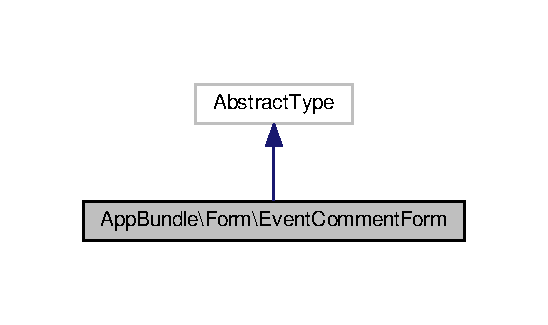
\includegraphics[width=263pt]{classAppBundle_1_1Form_1_1EventCommentForm__inherit__graph}
\end{center}
\end{figure}


Graphe de collaboration de App\+Bundle\textbackslash{}Form\textbackslash{}Event\+Comment\+Form\+:\nopagebreak
\begin{figure}[H]
\begin{center}
\leavevmode
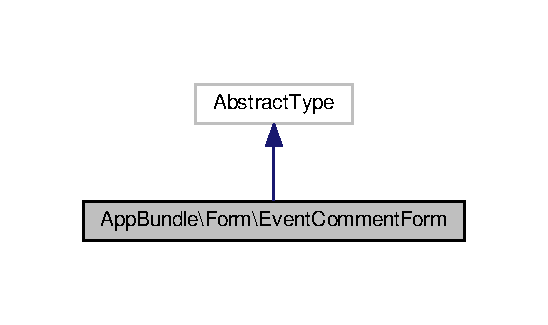
\includegraphics[width=263pt]{classAppBundle_1_1Form_1_1EventCommentForm__coll__graph}
\end{center}
\end{figure}
\subsection*{Fonctions membres publiques}
\begin{DoxyCompactItemize}
\item 
\mbox{\Hypertarget{classAppBundle_1_1Form_1_1EventCommentForm_a68bf60c94461bd12e1afcf17912b14e2}\label{classAppBundle_1_1Form_1_1EventCommentForm_a68bf60c94461bd12e1afcf17912b14e2}} 
{\bfseries build\+Form} (Form\+Builder\+Interface \$builder, array \$options)
\item 
\mbox{\Hypertarget{classAppBundle_1_1Form_1_1EventCommentForm_a0dc44ea425174d99e3de9e93b32ae077}\label{classAppBundle_1_1Form_1_1EventCommentForm_a0dc44ea425174d99e3de9e93b32ae077}} 
{\bfseries configure\+Options} (Options\+Resolver \$resolver)
\end{DoxyCompactItemize}


La documentation de cette classe a été générée à partir du fichier suivant \+:\begin{DoxyCompactItemize}
\item 
src/\+App\+Bundle/\+Form/Event\+Comment\+Form.\+php\end{DoxyCompactItemize}

\hypertarget{classAppBundle_1_1Repository_1_1EventCommentRepository}{}\section{Référence de la classe App\+Bundle\textbackslash{}Repository\textbackslash{}Event\+Comment\+Repository}
\label{classAppBundle_1_1Repository_1_1EventCommentRepository}\index{App\+Bundle\textbackslash{}\+Repository\textbackslash{}\+Event\+Comment\+Repository@{App\+Bundle\textbackslash{}\+Repository\textbackslash{}\+Event\+Comment\+Repository}}


Graphe d\textquotesingle{}héritage de App\+Bundle\textbackslash{}Repository\textbackslash{}Event\+Comment\+Repository\+:\nopagebreak
\begin{figure}[H]
\begin{center}
\leavevmode
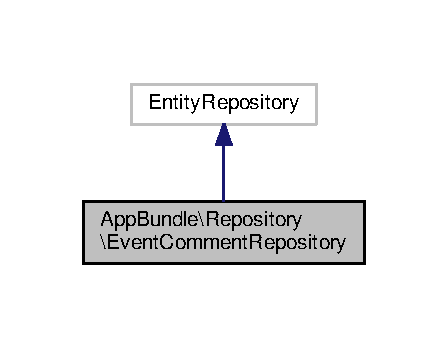
\includegraphics[width=215pt]{classAppBundle_1_1Repository_1_1EventCommentRepository__inherit__graph}
\end{center}
\end{figure}


Graphe de collaboration de App\+Bundle\textbackslash{}Repository\textbackslash{}Event\+Comment\+Repository\+:\nopagebreak
\begin{figure}[H]
\begin{center}
\leavevmode
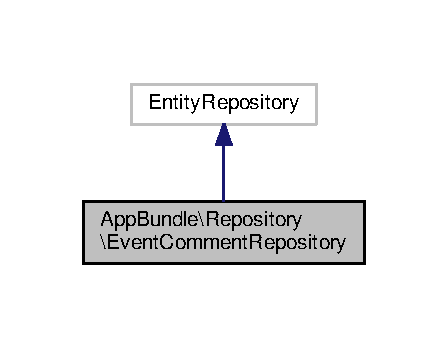
\includegraphics[width=215pt]{classAppBundle_1_1Repository_1_1EventCommentRepository__coll__graph}
\end{center}
\end{figure}


\subsection{Description détaillée}
\hyperlink{classAppBundle_1_1Repository_1_1EventCommentRepository}{Event\+Comment\+Repository}

This class was generated by the \hyperlink{namespaceAppBundle_1_1Doctrine}{Doctrine} O\+RM. Add your own custom repository methods below. 

La documentation de cette classe a été générée à partir du fichier suivant \+:\begin{DoxyCompactItemize}
\item 
src/\+App\+Bundle/\+Repository/Event\+Comment\+Repository.\+php\end{DoxyCompactItemize}

\hypertarget{classAppBundle_1_1Controller_1_1EventController}{}\section{Référence de la classe App\+Bundle\textbackslash{}Controller\textbackslash{}Event\+Controller}
\label{classAppBundle_1_1Controller_1_1EventController}\index{App\+Bundle\textbackslash{}\+Controller\textbackslash{}\+Event\+Controller@{App\+Bundle\textbackslash{}\+Controller\textbackslash{}\+Event\+Controller}}


Graphe d\textquotesingle{}héritage de App\+Bundle\textbackslash{}Controller\textbackslash{}Event\+Controller\+:\nopagebreak
\begin{figure}[H]
\begin{center}
\leavevmode
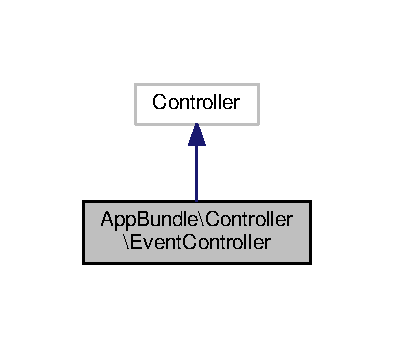
\includegraphics[width=189pt]{classAppBundle_1_1Controller_1_1EventController__inherit__graph}
\end{center}
\end{figure}


Graphe de collaboration de App\+Bundle\textbackslash{}Controller\textbackslash{}Event\+Controller\+:\nopagebreak
\begin{figure}[H]
\begin{center}
\leavevmode
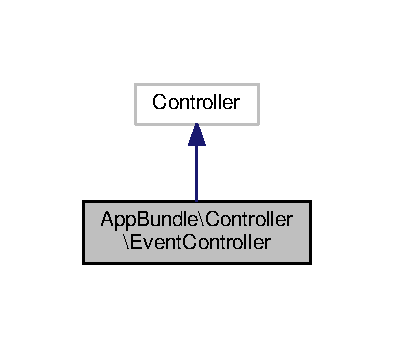
\includegraphics[width=189pt]{classAppBundle_1_1Controller_1_1EventController__coll__graph}
\end{center}
\end{figure}
\subsection*{Fonctions membres publiques}
\begin{DoxyCompactItemize}
\item 
\hyperlink{classAppBundle_1_1Controller_1_1EventController_a411287cd2df1b0571ac661d44a96b4be}{event\+Index\+Action} (Request \$request)
\item 
\hyperlink{classAppBundle_1_1Controller_1_1EventController_a31fbe84d7d41895928d28d9caca6cb07}{feed\+New\+Action} (Request \$request)
\item 
\hyperlink{classAppBundle_1_1Controller_1_1EventController_acd1acbb789cf2c9f5e4c9ba3e4b9e23f}{event\+Display\+Action} (Request \$request, \$event\+Id)
\item 
\hyperlink{classAppBundle_1_1Controller_1_1EventController_ad957c92b26d4d3bfbe4363f3997f0bc5}{event\+Delete\+Action} (Request \$request, \$event\+Id)
\end{DoxyCompactItemize}


\subsection{Documentation des fonctions membres}
\mbox{\Hypertarget{classAppBundle_1_1Controller_1_1EventController_ad957c92b26d4d3bfbe4363f3997f0bc5}\label{classAppBundle_1_1Controller_1_1EventController_ad957c92b26d4d3bfbe4363f3997f0bc5}} 
\index{App\+Bundle\+::\+Controller\+::\+Event\+Controller@{App\+Bundle\+::\+Controller\+::\+Event\+Controller}!event\+Delete\+Action@{event\+Delete\+Action}}
\index{event\+Delete\+Action@{event\+Delete\+Action}!App\+Bundle\+::\+Controller\+::\+Event\+Controller@{App\+Bundle\+::\+Controller\+::\+Event\+Controller}}
\subsubsection{\texorpdfstring{event\+Delete\+Action()}{eventDeleteAction()}}
{\footnotesize\ttfamily App\+Bundle\textbackslash{}\+Controller\textbackslash{}\+Event\+Controller\+::event\+Delete\+Action (\begin{DoxyParamCaption}\item[{Request}]{\$request,  }\item[{}]{\$event\+Id }\end{DoxyParamCaption})}

(\char`\"{}/delete/\{event\+Id\}\char`\"{}, name=\char`\"{}events-\/delete\char`\"{}) \mbox{\Hypertarget{classAppBundle_1_1Controller_1_1EventController_acd1acbb789cf2c9f5e4c9ba3e4b9e23f}\label{classAppBundle_1_1Controller_1_1EventController_acd1acbb789cf2c9f5e4c9ba3e4b9e23f}} 
\index{App\+Bundle\+::\+Controller\+::\+Event\+Controller@{App\+Bundle\+::\+Controller\+::\+Event\+Controller}!event\+Display\+Action@{event\+Display\+Action}}
\index{event\+Display\+Action@{event\+Display\+Action}!App\+Bundle\+::\+Controller\+::\+Event\+Controller@{App\+Bundle\+::\+Controller\+::\+Event\+Controller}}
\subsubsection{\texorpdfstring{event\+Display\+Action()}{eventDisplayAction()}}
{\footnotesize\ttfamily App\+Bundle\textbackslash{}\+Controller\textbackslash{}\+Event\+Controller\+::event\+Display\+Action (\begin{DoxyParamCaption}\item[{Request}]{\$request,  }\item[{}]{\$event\+Id }\end{DoxyParamCaption})}

(\char`\"{}/view/\{event\+Id\}\char`\"{}, name=\char`\"{}events-\/view\char`\"{}) \mbox{\Hypertarget{classAppBundle_1_1Controller_1_1EventController_a411287cd2df1b0571ac661d44a96b4be}\label{classAppBundle_1_1Controller_1_1EventController_a411287cd2df1b0571ac661d44a96b4be}} 
\index{App\+Bundle\+::\+Controller\+::\+Event\+Controller@{App\+Bundle\+::\+Controller\+::\+Event\+Controller}!event\+Index\+Action@{event\+Index\+Action}}
\index{event\+Index\+Action@{event\+Index\+Action}!App\+Bundle\+::\+Controller\+::\+Event\+Controller@{App\+Bundle\+::\+Controller\+::\+Event\+Controller}}
\subsubsection{\texorpdfstring{event\+Index\+Action()}{eventIndexAction()}}
{\footnotesize\ttfamily App\+Bundle\textbackslash{}\+Controller\textbackslash{}\+Event\+Controller\+::event\+Index\+Action (\begin{DoxyParamCaption}\item[{Request}]{\$request }\end{DoxyParamCaption})}

(\char`\"{}/\char`\"{}, name=\char`\"{}events-\/index\char`\"{}) \mbox{\Hypertarget{classAppBundle_1_1Controller_1_1EventController_a31fbe84d7d41895928d28d9caca6cb07}\label{classAppBundle_1_1Controller_1_1EventController_a31fbe84d7d41895928d28d9caca6cb07}} 
\index{App\+Bundle\+::\+Controller\+::\+Event\+Controller@{App\+Bundle\+::\+Controller\+::\+Event\+Controller}!feed\+New\+Action@{feed\+New\+Action}}
\index{feed\+New\+Action@{feed\+New\+Action}!App\+Bundle\+::\+Controller\+::\+Event\+Controller@{App\+Bundle\+::\+Controller\+::\+Event\+Controller}}
\subsubsection{\texorpdfstring{feed\+New\+Action()}{feedNewAction()}}
{\footnotesize\ttfamily App\+Bundle\textbackslash{}\+Controller\textbackslash{}\+Event\+Controller\+::feed\+New\+Action (\begin{DoxyParamCaption}\item[{Request}]{\$request }\end{DoxyParamCaption})}

(\char`\"{}/new\char`\"{}, name=\char`\"{}events-\/new\char`\"{}) 

La documentation de cette classe a été générée à partir du fichier suivant \+:\begin{DoxyCompactItemize}
\item 
src/\+App\+Bundle/\+Controller/Event\+Controller.\+php\end{DoxyCompactItemize}

\hypertarget{classAppBundle_1_1Repository_1_1EventRepository}{}\section{Référence de la classe App\+Bundle\textbackslash{}Repository\textbackslash{}Event\+Repository}
\label{classAppBundle_1_1Repository_1_1EventRepository}\index{App\+Bundle\textbackslash{}\+Repository\textbackslash{}\+Event\+Repository@{App\+Bundle\textbackslash{}\+Repository\textbackslash{}\+Event\+Repository}}


Graphe d\textquotesingle{}héritage de App\+Bundle\textbackslash{}Repository\textbackslash{}Event\+Repository\+:\nopagebreak
\begin{figure}[H]
\begin{center}
\leavevmode
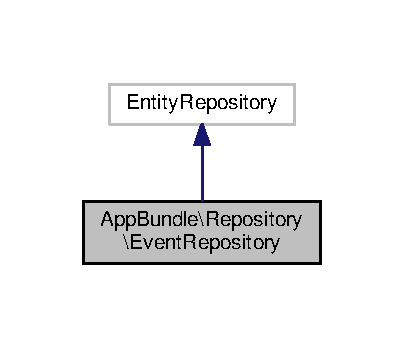
\includegraphics[width=194pt]{classAppBundle_1_1Repository_1_1EventRepository__inherit__graph}
\end{center}
\end{figure}


Graphe de collaboration de App\+Bundle\textbackslash{}Repository\textbackslash{}Event\+Repository\+:\nopagebreak
\begin{figure}[H]
\begin{center}
\leavevmode
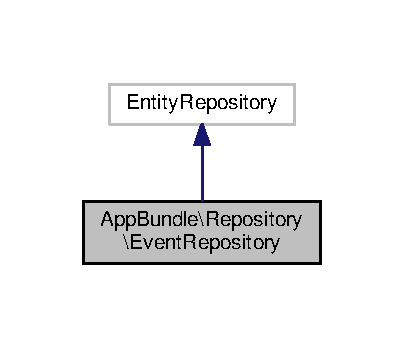
\includegraphics[width=194pt]{classAppBundle_1_1Repository_1_1EventRepository__coll__graph}
\end{center}
\end{figure}


\subsection{Description détaillée}
\hyperlink{classAppBundle_1_1Repository_1_1EventRepository}{Event\+Repository}

This class was generated by the \hyperlink{namespaceAppBundle_1_1Doctrine}{Doctrine} O\+RM. Add your own custom repository methods below. 

La documentation de cette classe a été générée à partir du fichier suivant \+:\begin{DoxyCompactItemize}
\item 
src/\+App\+Bundle/\+Repository/Event\+Repository.\+php\end{DoxyCompactItemize}

\hypertarget{classAppBundle_1_1Twig_1_1ExcerptExtension}{}\section{Référence de la classe App\+Bundle\textbackslash{}Twig\textbackslash{}Excerpt\+Extension}
\label{classAppBundle_1_1Twig_1_1ExcerptExtension}\index{App\+Bundle\textbackslash{}\+Twig\textbackslash{}\+Excerpt\+Extension@{App\+Bundle\textbackslash{}\+Twig\textbackslash{}\+Excerpt\+Extension}}


Graphe d\textquotesingle{}héritage de App\+Bundle\textbackslash{}Twig\textbackslash{}Excerpt\+Extension\+:\nopagebreak
\begin{figure}[H]
\begin{center}
\leavevmode
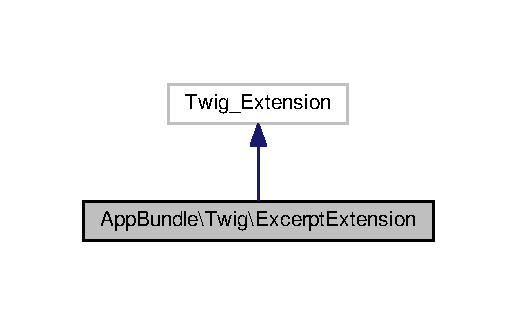
\includegraphics[width=248pt]{classAppBundle_1_1Twig_1_1ExcerptExtension__inherit__graph}
\end{center}
\end{figure}


Graphe de collaboration de App\+Bundle\textbackslash{}Twig\textbackslash{}Excerpt\+Extension\+:\nopagebreak
\begin{figure}[H]
\begin{center}
\leavevmode
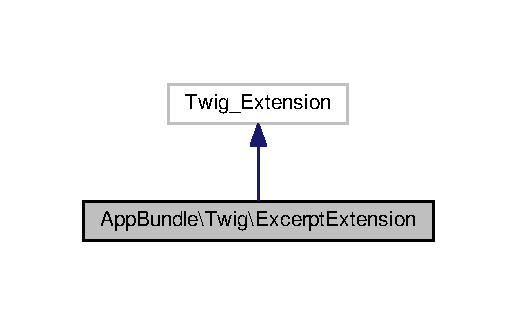
\includegraphics[width=248pt]{classAppBundle_1_1Twig_1_1ExcerptExtension__coll__graph}
\end{center}
\end{figure}
\subsection*{Fonctions membres publiques}
\begin{DoxyCompactItemize}
\item 
\hyperlink{classAppBundle_1_1Twig_1_1ExcerptExtension_aa607e8e11c8b6ac43c3996e8f86b4544}{get\+Filters} ()
\item 
\hyperlink{classAppBundle_1_1Twig_1_1ExcerptExtension_a60d918a9302749cdc79dd680f96955a1}{excerpt} (?string \$content, int \$max\+Length=200)
\end{DoxyCompactItemize}


\subsection{Documentation des fonctions membres}
\mbox{\Hypertarget{classAppBundle_1_1Twig_1_1ExcerptExtension_a60d918a9302749cdc79dd680f96955a1}\label{classAppBundle_1_1Twig_1_1ExcerptExtension_a60d918a9302749cdc79dd680f96955a1}} 
\index{App\+Bundle\+::\+Twig\+::\+Excerpt\+Extension@{App\+Bundle\+::\+Twig\+::\+Excerpt\+Extension}!excerpt@{excerpt}}
\index{excerpt@{excerpt}!App\+Bundle\+::\+Twig\+::\+Excerpt\+Extension@{App\+Bundle\+::\+Twig\+::\+Excerpt\+Extension}}
\subsubsection{\texorpdfstring{excerpt()}{excerpt()}}
{\footnotesize\ttfamily App\+Bundle\textbackslash{}\+Twig\textbackslash{}\+Excerpt\+Extension\+::excerpt (\begin{DoxyParamCaption}\item[{?string}]{\$content,  }\item[{int}]{\$max\+Length = {\ttfamily 200} }\end{DoxyParamCaption})}

Renvoie un extrait du contenu 
\begin{DoxyParams}[1]{Paramètres}
string & {\em \$content} & \\
\hline
int & {\em \$max\+Length} & \\
\hline
\end{DoxyParams}
\begin{DoxyReturn}{Renvoie}
string 
\end{DoxyReturn}
\mbox{\Hypertarget{classAppBundle_1_1Twig_1_1ExcerptExtension_aa607e8e11c8b6ac43c3996e8f86b4544}\label{classAppBundle_1_1Twig_1_1ExcerptExtension_aa607e8e11c8b6ac43c3996e8f86b4544}} 
\index{App\+Bundle\+::\+Twig\+::\+Excerpt\+Extension@{App\+Bundle\+::\+Twig\+::\+Excerpt\+Extension}!get\+Filters@{get\+Filters}}
\index{get\+Filters@{get\+Filters}!App\+Bundle\+::\+Twig\+::\+Excerpt\+Extension@{App\+Bundle\+::\+Twig\+::\+Excerpt\+Extension}}
\subsubsection{\texorpdfstring{get\+Filters()}{getFilters()}}
{\footnotesize\ttfamily App\+Bundle\textbackslash{}\+Twig\textbackslash{}\+Excerpt\+Extension\+::get\+Filters (\begin{DoxyParamCaption}{ }\end{DoxyParamCaption})}

\begin{DoxyReturn}{Renvoie}
array 
\end{DoxyReturn}


La documentation de cette classe a été générée à partir du fichier suivant \+:\begin{DoxyCompactItemize}
\item 
src/\+App\+Bundle/\+Twig/Excerpt\+Extension.\+php\end{DoxyCompactItemize}

\hypertarget{classAppBundle_1_1Entity_1_1Favorite}{}\section{Référence de la classe App\+Bundle\textbackslash{}Entity\textbackslash{}Favorite}
\label{classAppBundle_1_1Entity_1_1Favorite}\index{App\+Bundle\textbackslash{}\+Entity\textbackslash{}\+Favorite@{App\+Bundle\textbackslash{}\+Entity\textbackslash{}\+Favorite}}
\subsection*{Fonctions membres publiques}
\begin{DoxyCompactItemize}
\item 
\hyperlink{classAppBundle_1_1Entity_1_1Favorite_add4985c90fac741fcb1a5026bd8551e4}{get\+Id} ()
\item 
\hyperlink{classAppBundle_1_1Entity_1_1Favorite_a22180c0120b1661263dc8e3e2053c9cc}{set\+Name} (\$name)
\item 
\hyperlink{classAppBundle_1_1Entity_1_1Favorite_a66cbf797b0af61339eb9ece8b36ecc1c}{get\+Name} ()
\item 
\hyperlink{classAppBundle_1_1Entity_1_1Favorite_afddba3b312caa97af160fdebc187ad4d}{set\+Lat} (\$lat)
\item 
\hyperlink{classAppBundle_1_1Entity_1_1Favorite_a0092e20408e1e56065c3ffc90a56acf7}{get\+Lat} ()
\item 
\hyperlink{classAppBundle_1_1Entity_1_1Favorite_a8dcb451f06346ea01b131bfc174821dd}{set\+Lon} (\$lon)
\item 
\hyperlink{classAppBundle_1_1Entity_1_1Favorite_a7f467c2a1e0e93b1afcd8710cccd97b7}{get\+Lon} ()
\item 
\hyperlink{classAppBundle_1_1Entity_1_1Favorite_a565975ee6c451fb15aad99e50746f907}{set\+User} (\textbackslash{}\hyperlink{classAppBundle_1_1Entity_1_1User}{App\+Bundle\textbackslash{}\+Entity\textbackslash{}\+User} \$user)
\item 
\hyperlink{classAppBundle_1_1Entity_1_1Favorite_a69db26313aefb7b377ba8e482e6fb0f0}{get\+User} ()
\item 
\hyperlink{classAppBundle_1_1Entity_1_1Favorite_ace4e1309956105ce3511efe64ae79287}{set\+Owm\+Id} (\$owm\+Id)
\item 
\hyperlink{classAppBundle_1_1Entity_1_1Favorite_aca73f8e626c8cf7eb6cdf9a2843e15fe}{get\+Owm\+Id} ()
\item 
\hyperlink{classAppBundle_1_1Entity_1_1Favorite_a2c0e6fb12140e51b95c906ac86b952b9}{set\+Map\+Id} (\$map\+Id)
\item 
\hyperlink{classAppBundle_1_1Entity_1_1Favorite_abbe92666121b77689ef6fc6e137e6a16}{get\+Map\+Id} ()
\item 
\hyperlink{classAppBundle_1_1Entity_1_1Favorite_af6a48e472097646cfa0d79c3162f5cbf}{set\+Location} (\textbackslash{}\hyperlink{classAppBundle_1_1Entity_1_1Location}{App\+Bundle\textbackslash{}\+Entity\textbackslash{}\+Location} \$location)
\item 
\hyperlink{classAppBundle_1_1Entity_1_1Favorite_a2a8222cd57c851020fbedc64398e8744}{get\+Location} ()
\end{DoxyCompactItemize}


\subsection{Description détaillée}
\hyperlink{classAppBundle_1_1Entity_1_1Favorite}{Favorite}

(name=\char`\"{}favorite\char`\"{}) (repository\+Class=\char`\"{}\+App\+Bundle\textbackslash{}\+Repository\textbackslash{}\+Favorite\+Repository\char`\"{}) 

\subsection{Documentation des fonctions membres}
\mbox{\Hypertarget{classAppBundle_1_1Entity_1_1Favorite_add4985c90fac741fcb1a5026bd8551e4}\label{classAppBundle_1_1Entity_1_1Favorite_add4985c90fac741fcb1a5026bd8551e4}} 
\index{App\+Bundle\+::\+Entity\+::\+Favorite@{App\+Bundle\+::\+Entity\+::\+Favorite}!get\+Id@{get\+Id}}
\index{get\+Id@{get\+Id}!App\+Bundle\+::\+Entity\+::\+Favorite@{App\+Bundle\+::\+Entity\+::\+Favorite}}
\subsubsection{\texorpdfstring{get\+Id()}{getId()}}
{\footnotesize\ttfamily App\+Bundle\textbackslash{}\+Entity\textbackslash{}\+Favorite\+::get\+Id (\begin{DoxyParamCaption}{ }\end{DoxyParamCaption})}

Get id

\begin{DoxyReturn}{Renvoie}
int 
\end{DoxyReturn}
\mbox{\Hypertarget{classAppBundle_1_1Entity_1_1Favorite_a0092e20408e1e56065c3ffc90a56acf7}\label{classAppBundle_1_1Entity_1_1Favorite_a0092e20408e1e56065c3ffc90a56acf7}} 
\index{App\+Bundle\+::\+Entity\+::\+Favorite@{App\+Bundle\+::\+Entity\+::\+Favorite}!get\+Lat@{get\+Lat}}
\index{get\+Lat@{get\+Lat}!App\+Bundle\+::\+Entity\+::\+Favorite@{App\+Bundle\+::\+Entity\+::\+Favorite}}
\subsubsection{\texorpdfstring{get\+Lat()}{getLat()}}
{\footnotesize\ttfamily App\+Bundle\textbackslash{}\+Entity\textbackslash{}\+Favorite\+::get\+Lat (\begin{DoxyParamCaption}{ }\end{DoxyParamCaption})}

Get lat

\begin{DoxyReturn}{Renvoie}
float 
\end{DoxyReturn}
\mbox{\Hypertarget{classAppBundle_1_1Entity_1_1Favorite_a2a8222cd57c851020fbedc64398e8744}\label{classAppBundle_1_1Entity_1_1Favorite_a2a8222cd57c851020fbedc64398e8744}} 
\index{App\+Bundle\+::\+Entity\+::\+Favorite@{App\+Bundle\+::\+Entity\+::\+Favorite}!get\+Location@{get\+Location}}
\index{get\+Location@{get\+Location}!App\+Bundle\+::\+Entity\+::\+Favorite@{App\+Bundle\+::\+Entity\+::\+Favorite}}
\subsubsection{\texorpdfstring{get\+Location()}{getLocation()}}
{\footnotesize\ttfamily App\+Bundle\textbackslash{}\+Entity\textbackslash{}\+Favorite\+::get\+Location (\begin{DoxyParamCaption}{ }\end{DoxyParamCaption})}

Get location

\begin{DoxyReturn}{Renvoie}

\end{DoxyReturn}
\mbox{\Hypertarget{classAppBundle_1_1Entity_1_1Favorite_a7f467c2a1e0e93b1afcd8710cccd97b7}\label{classAppBundle_1_1Entity_1_1Favorite_a7f467c2a1e0e93b1afcd8710cccd97b7}} 
\index{App\+Bundle\+::\+Entity\+::\+Favorite@{App\+Bundle\+::\+Entity\+::\+Favorite}!get\+Lon@{get\+Lon}}
\index{get\+Lon@{get\+Lon}!App\+Bundle\+::\+Entity\+::\+Favorite@{App\+Bundle\+::\+Entity\+::\+Favorite}}
\subsubsection{\texorpdfstring{get\+Lon()}{getLon()}}
{\footnotesize\ttfamily App\+Bundle\textbackslash{}\+Entity\textbackslash{}\+Favorite\+::get\+Lon (\begin{DoxyParamCaption}{ }\end{DoxyParamCaption})}

Get lon

\begin{DoxyReturn}{Renvoie}
float 
\end{DoxyReturn}
\mbox{\Hypertarget{classAppBundle_1_1Entity_1_1Favorite_abbe92666121b77689ef6fc6e137e6a16}\label{classAppBundle_1_1Entity_1_1Favorite_abbe92666121b77689ef6fc6e137e6a16}} 
\index{App\+Bundle\+::\+Entity\+::\+Favorite@{App\+Bundle\+::\+Entity\+::\+Favorite}!get\+Map\+Id@{get\+Map\+Id}}
\index{get\+Map\+Id@{get\+Map\+Id}!App\+Bundle\+::\+Entity\+::\+Favorite@{App\+Bundle\+::\+Entity\+::\+Favorite}}
\subsubsection{\texorpdfstring{get\+Map\+Id()}{getMapId()}}
{\footnotesize\ttfamily App\+Bundle\textbackslash{}\+Entity\textbackslash{}\+Favorite\+::get\+Map\+Id (\begin{DoxyParamCaption}{ }\end{DoxyParamCaption})}

Get map\+Id

\begin{DoxyReturn}{Renvoie}
integer 
\end{DoxyReturn}
\mbox{\Hypertarget{classAppBundle_1_1Entity_1_1Favorite_a66cbf797b0af61339eb9ece8b36ecc1c}\label{classAppBundle_1_1Entity_1_1Favorite_a66cbf797b0af61339eb9ece8b36ecc1c}} 
\index{App\+Bundle\+::\+Entity\+::\+Favorite@{App\+Bundle\+::\+Entity\+::\+Favorite}!get\+Name@{get\+Name}}
\index{get\+Name@{get\+Name}!App\+Bundle\+::\+Entity\+::\+Favorite@{App\+Bundle\+::\+Entity\+::\+Favorite}}
\subsubsection{\texorpdfstring{get\+Name()}{getName()}}
{\footnotesize\ttfamily App\+Bundle\textbackslash{}\+Entity\textbackslash{}\+Favorite\+::get\+Name (\begin{DoxyParamCaption}{ }\end{DoxyParamCaption})}

Get name

\begin{DoxyReturn}{Renvoie}
string 
\end{DoxyReturn}
\mbox{\Hypertarget{classAppBundle_1_1Entity_1_1Favorite_aca73f8e626c8cf7eb6cdf9a2843e15fe}\label{classAppBundle_1_1Entity_1_1Favorite_aca73f8e626c8cf7eb6cdf9a2843e15fe}} 
\index{App\+Bundle\+::\+Entity\+::\+Favorite@{App\+Bundle\+::\+Entity\+::\+Favorite}!get\+Owm\+Id@{get\+Owm\+Id}}
\index{get\+Owm\+Id@{get\+Owm\+Id}!App\+Bundle\+::\+Entity\+::\+Favorite@{App\+Bundle\+::\+Entity\+::\+Favorite}}
\subsubsection{\texorpdfstring{get\+Owm\+Id()}{getOwmId()}}
{\footnotesize\ttfamily App\+Bundle\textbackslash{}\+Entity\textbackslash{}\+Favorite\+::get\+Owm\+Id (\begin{DoxyParamCaption}{ }\end{DoxyParamCaption})}

Get owm\+Id

\begin{DoxyReturn}{Renvoie}
integer 
\end{DoxyReturn}
\mbox{\Hypertarget{classAppBundle_1_1Entity_1_1Favorite_a69db26313aefb7b377ba8e482e6fb0f0}\label{classAppBundle_1_1Entity_1_1Favorite_a69db26313aefb7b377ba8e482e6fb0f0}} 
\index{App\+Bundle\+::\+Entity\+::\+Favorite@{App\+Bundle\+::\+Entity\+::\+Favorite}!get\+User@{get\+User}}
\index{get\+User@{get\+User}!App\+Bundle\+::\+Entity\+::\+Favorite@{App\+Bundle\+::\+Entity\+::\+Favorite}}
\subsubsection{\texorpdfstring{get\+User()}{getUser()}}
{\footnotesize\ttfamily App\+Bundle\textbackslash{}\+Entity\textbackslash{}\+Favorite\+::get\+User (\begin{DoxyParamCaption}{ }\end{DoxyParamCaption})}

Get user

\begin{DoxyReturn}{Renvoie}

\end{DoxyReturn}
\mbox{\Hypertarget{classAppBundle_1_1Entity_1_1Favorite_afddba3b312caa97af160fdebc187ad4d}\label{classAppBundle_1_1Entity_1_1Favorite_afddba3b312caa97af160fdebc187ad4d}} 
\index{App\+Bundle\+::\+Entity\+::\+Favorite@{App\+Bundle\+::\+Entity\+::\+Favorite}!set\+Lat@{set\+Lat}}
\index{set\+Lat@{set\+Lat}!App\+Bundle\+::\+Entity\+::\+Favorite@{App\+Bundle\+::\+Entity\+::\+Favorite}}
\subsubsection{\texorpdfstring{set\+Lat()}{setLat()}}
{\footnotesize\ttfamily App\+Bundle\textbackslash{}\+Entity\textbackslash{}\+Favorite\+::set\+Lat (\begin{DoxyParamCaption}\item[{}]{\$lat }\end{DoxyParamCaption})}

Set lat


\begin{DoxyParams}[1]{Paramètres}
float & {\em \$lat} & \\
\hline
\end{DoxyParams}
\begin{DoxyReturn}{Renvoie}
\hyperlink{classAppBundle_1_1Entity_1_1Favorite}{Favorite} 
\end{DoxyReturn}
\mbox{\Hypertarget{classAppBundle_1_1Entity_1_1Favorite_af6a48e472097646cfa0d79c3162f5cbf}\label{classAppBundle_1_1Entity_1_1Favorite_af6a48e472097646cfa0d79c3162f5cbf}} 
\index{App\+Bundle\+::\+Entity\+::\+Favorite@{App\+Bundle\+::\+Entity\+::\+Favorite}!set\+Location@{set\+Location}}
\index{set\+Location@{set\+Location}!App\+Bundle\+::\+Entity\+::\+Favorite@{App\+Bundle\+::\+Entity\+::\+Favorite}}
\subsubsection{\texorpdfstring{set\+Location()}{setLocation()}}
{\footnotesize\ttfamily App\+Bundle\textbackslash{}\+Entity\textbackslash{}\+Favorite\+::set\+Location (\begin{DoxyParamCaption}\item[{\textbackslash{}\hyperlink{classAppBundle_1_1Entity_1_1Location}{App\+Bundle\textbackslash{}\+Entity\textbackslash{}\+Location}}]{\$location }\end{DoxyParamCaption})}

Set location


\begin{DoxyParams}[1]{Paramètres}
\textbackslash{}\+App\+Bundle\textbackslash{}\+Entity\textbackslash{}\+Location & {\em \$location} & \\
\hline
\end{DoxyParams}
\begin{DoxyReturn}{Renvoie}
\hyperlink{classAppBundle_1_1Entity_1_1Favorite}{Favorite} 
\end{DoxyReturn}
\mbox{\Hypertarget{classAppBundle_1_1Entity_1_1Favorite_a8dcb451f06346ea01b131bfc174821dd}\label{classAppBundle_1_1Entity_1_1Favorite_a8dcb451f06346ea01b131bfc174821dd}} 
\index{App\+Bundle\+::\+Entity\+::\+Favorite@{App\+Bundle\+::\+Entity\+::\+Favorite}!set\+Lon@{set\+Lon}}
\index{set\+Lon@{set\+Lon}!App\+Bundle\+::\+Entity\+::\+Favorite@{App\+Bundle\+::\+Entity\+::\+Favorite}}
\subsubsection{\texorpdfstring{set\+Lon()}{setLon()}}
{\footnotesize\ttfamily App\+Bundle\textbackslash{}\+Entity\textbackslash{}\+Favorite\+::set\+Lon (\begin{DoxyParamCaption}\item[{}]{\$lon }\end{DoxyParamCaption})}

Set lon


\begin{DoxyParams}[1]{Paramètres}
float & {\em \$lon} & \\
\hline
\end{DoxyParams}
\begin{DoxyReturn}{Renvoie}
\hyperlink{classAppBundle_1_1Entity_1_1Favorite}{Favorite} 
\end{DoxyReturn}
\mbox{\Hypertarget{classAppBundle_1_1Entity_1_1Favorite_a2c0e6fb12140e51b95c906ac86b952b9}\label{classAppBundle_1_1Entity_1_1Favorite_a2c0e6fb12140e51b95c906ac86b952b9}} 
\index{App\+Bundle\+::\+Entity\+::\+Favorite@{App\+Bundle\+::\+Entity\+::\+Favorite}!set\+Map\+Id@{set\+Map\+Id}}
\index{set\+Map\+Id@{set\+Map\+Id}!App\+Bundle\+::\+Entity\+::\+Favorite@{App\+Bundle\+::\+Entity\+::\+Favorite}}
\subsubsection{\texorpdfstring{set\+Map\+Id()}{setMapId()}}
{\footnotesize\ttfamily App\+Bundle\textbackslash{}\+Entity\textbackslash{}\+Favorite\+::set\+Map\+Id (\begin{DoxyParamCaption}\item[{}]{\$map\+Id }\end{DoxyParamCaption})}

Set map\+Id


\begin{DoxyParams}[1]{Paramètres}
integer & {\em \$map\+Id} & \\
\hline
\end{DoxyParams}
\begin{DoxyReturn}{Renvoie}
\hyperlink{classAppBundle_1_1Entity_1_1Favorite}{Favorite} 
\end{DoxyReturn}
\mbox{\Hypertarget{classAppBundle_1_1Entity_1_1Favorite_a22180c0120b1661263dc8e3e2053c9cc}\label{classAppBundle_1_1Entity_1_1Favorite_a22180c0120b1661263dc8e3e2053c9cc}} 
\index{App\+Bundle\+::\+Entity\+::\+Favorite@{App\+Bundle\+::\+Entity\+::\+Favorite}!set\+Name@{set\+Name}}
\index{set\+Name@{set\+Name}!App\+Bundle\+::\+Entity\+::\+Favorite@{App\+Bundle\+::\+Entity\+::\+Favorite}}
\subsubsection{\texorpdfstring{set\+Name()}{setName()}}
{\footnotesize\ttfamily App\+Bundle\textbackslash{}\+Entity\textbackslash{}\+Favorite\+::set\+Name (\begin{DoxyParamCaption}\item[{}]{\$name }\end{DoxyParamCaption})}

Set name


\begin{DoxyParams}[1]{Paramètres}
string & {\em \$name} & \\
\hline
\end{DoxyParams}
\begin{DoxyReturn}{Renvoie}
\hyperlink{classAppBundle_1_1Entity_1_1Favorite}{Favorite} 
\end{DoxyReturn}
\mbox{\Hypertarget{classAppBundle_1_1Entity_1_1Favorite_ace4e1309956105ce3511efe64ae79287}\label{classAppBundle_1_1Entity_1_1Favorite_ace4e1309956105ce3511efe64ae79287}} 
\index{App\+Bundle\+::\+Entity\+::\+Favorite@{App\+Bundle\+::\+Entity\+::\+Favorite}!set\+Owm\+Id@{set\+Owm\+Id}}
\index{set\+Owm\+Id@{set\+Owm\+Id}!App\+Bundle\+::\+Entity\+::\+Favorite@{App\+Bundle\+::\+Entity\+::\+Favorite}}
\subsubsection{\texorpdfstring{set\+Owm\+Id()}{setOwmId()}}
{\footnotesize\ttfamily App\+Bundle\textbackslash{}\+Entity\textbackslash{}\+Favorite\+::set\+Owm\+Id (\begin{DoxyParamCaption}\item[{}]{\$owm\+Id }\end{DoxyParamCaption})}

Set owm\+Id


\begin{DoxyParams}[1]{Paramètres}
integer & {\em \$owm\+Id} & \\
\hline
\end{DoxyParams}
\begin{DoxyReturn}{Renvoie}
\hyperlink{classAppBundle_1_1Entity_1_1Favorite}{Favorite} 
\end{DoxyReturn}
\mbox{\Hypertarget{classAppBundle_1_1Entity_1_1Favorite_a565975ee6c451fb15aad99e50746f907}\label{classAppBundle_1_1Entity_1_1Favorite_a565975ee6c451fb15aad99e50746f907}} 
\index{App\+Bundle\+::\+Entity\+::\+Favorite@{App\+Bundle\+::\+Entity\+::\+Favorite}!set\+User@{set\+User}}
\index{set\+User@{set\+User}!App\+Bundle\+::\+Entity\+::\+Favorite@{App\+Bundle\+::\+Entity\+::\+Favorite}}
\subsubsection{\texorpdfstring{set\+User()}{setUser()}}
{\footnotesize\ttfamily App\+Bundle\textbackslash{}\+Entity\textbackslash{}\+Favorite\+::set\+User (\begin{DoxyParamCaption}\item[{\textbackslash{}\hyperlink{classAppBundle_1_1Entity_1_1User}{App\+Bundle\textbackslash{}\+Entity\textbackslash{}\+User}}]{\$user }\end{DoxyParamCaption})}

Set user


\begin{DoxyParams}[1]{Paramètres}
\textbackslash{}\+App\+Bundle\textbackslash{}\+Entity\textbackslash{}\+User & {\em \$user} & \\
\hline
\end{DoxyParams}
\begin{DoxyReturn}{Renvoie}
\hyperlink{classAppBundle_1_1Entity_1_1Favorite}{Favorite} 
\end{DoxyReturn}


La documentation de cette classe a été générée à partir du fichier suivant \+:\begin{DoxyCompactItemize}
\item 
src/\+App\+Bundle/\+Entity/Favorite.\+php\end{DoxyCompactItemize}

\hypertarget{classAppBundle_1_1Repository_1_1FavoriteRepository}{}\section{Référence de la classe App\+Bundle\textbackslash{}Repository\textbackslash{}Favorite\+Repository}
\label{classAppBundle_1_1Repository_1_1FavoriteRepository}\index{App\+Bundle\textbackslash{}\+Repository\textbackslash{}\+Favorite\+Repository@{App\+Bundle\textbackslash{}\+Repository\textbackslash{}\+Favorite\+Repository}}


Graphe d\textquotesingle{}héritage de App\+Bundle\textbackslash{}Repository\textbackslash{}Favorite\+Repository\+:\nopagebreak
\begin{figure}[H]
\begin{center}
\leavevmode
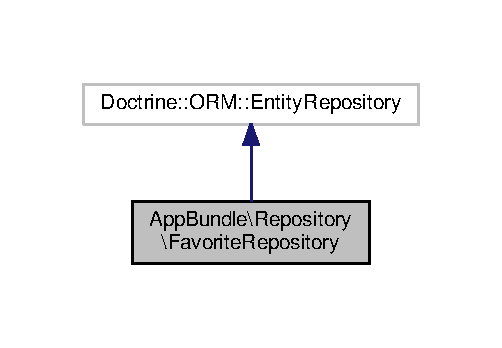
\includegraphics[width=241pt]{classAppBundle_1_1Repository_1_1FavoriteRepository__inherit__graph}
\end{center}
\end{figure}


Graphe de collaboration de App\+Bundle\textbackslash{}Repository\textbackslash{}Favorite\+Repository\+:\nopagebreak
\begin{figure}[H]
\begin{center}
\leavevmode
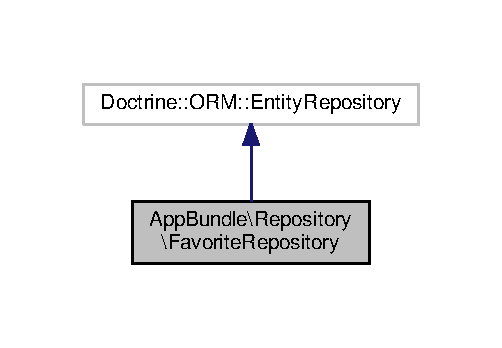
\includegraphics[width=241pt]{classAppBundle_1_1Repository_1_1FavoriteRepository__coll__graph}
\end{center}
\end{figure}


\subsection{Description détaillée}
\hyperlink{classAppBundle_1_1Repository_1_1FavoriteRepository}{Favorite\+Repository}

This class was generated by the \hyperlink{namespaceAppBundle_1_1Doctrine}{Doctrine} O\+RM. Add your own custom repository methods below. 

La documentation de cette classe a été générée à partir du fichier suivant \+:\begin{DoxyCompactItemize}
\item 
src/\+App\+Bundle/\+Repository/Favorite\+Repository.\+php\end{DoxyCompactItemize}

\hypertarget{classAppBundle_1_1Entity_1_1Location}{}\section{Référence de la classe App\+Bundle\textbackslash{}Entity\textbackslash{}Location}
\label{classAppBundle_1_1Entity_1_1Location}\index{App\+Bundle\textbackslash{}\+Entity\textbackslash{}\+Location@{App\+Bundle\textbackslash{}\+Entity\textbackslash{}\+Location}}
\subsection*{Fonctions membres publiques}
\begin{DoxyCompactItemize}
\item 
\hyperlink{classAppBundle_1_1Entity_1_1Location_a40cd226faaa21283918bcbebfb8d9729}{get\+Id} ()
\item 
\hyperlink{classAppBundle_1_1Entity_1_1Location_aec02b0397a895b43863dc95118eca59d}{set\+Latitude} (\$latitude)
\item 
\hyperlink{classAppBundle_1_1Entity_1_1Location_a03576959d91ad5db3071a2b28430ca59}{get\+Latitude} ()
\item 
\hyperlink{classAppBundle_1_1Entity_1_1Location_a0591ba9da720d3334013549916c3347b}{set\+Longitude} (\$longitude)
\item 
\hyperlink{classAppBundle_1_1Entity_1_1Location_a5af4e443cb4e99ed95981276f451450b}{get\+Longitude} ()
\item 
\hyperlink{classAppBundle_1_1Entity_1_1Location_aaee06ec64eadc141b27c883faab92552}{\+\_\+\+\_\+construct} ()
\item 
\hyperlink{classAppBundle_1_1Entity_1_1Location_a49b47d7c0be25471d81d1ae3e31ba448}{add\+Review} (\textbackslash{}\hyperlink{classAppBundle_1_1Entity_1_1Review}{App\+Bundle\textbackslash{}\+Entity\textbackslash{}\+Review} \$review)
\item 
\hyperlink{classAppBundle_1_1Entity_1_1Location_a42339fbc46751d310a10c650b8b4d797}{remove\+Review} (\textbackslash{}\hyperlink{classAppBundle_1_1Entity_1_1Review}{App\+Bundle\textbackslash{}\+Entity\textbackslash{}\+Review} \$review)
\item 
\hyperlink{classAppBundle_1_1Entity_1_1Location_a6a8cdadd950886f414ea7c456e8e4a5e}{get\+Reviews} ()
\item 
\hyperlink{classAppBundle_1_1Entity_1_1Location_a9a0d9075d1a1fa5e2efea262412045d0}{set\+Name} (\$name)
\item 
\hyperlink{classAppBundle_1_1Entity_1_1Location_af45b7253351a49a59704ff76bf65d945}{get\+Name} ()
\end{DoxyCompactItemize}


\subsection{Description détaillée}
\hyperlink{classAppBundle_1_1Entity_1_1Location}{Location}

(name=\char`\"{}location\char`\"{}) (repository\+Class=\char`\"{}\+App\+Bundle\textbackslash{}\+Repository\textbackslash{}\+Location\+Repository\char`\"{}) 

\subsection{Documentation des constructeurs et destructeur}
\mbox{\Hypertarget{classAppBundle_1_1Entity_1_1Location_aaee06ec64eadc141b27c883faab92552}\label{classAppBundle_1_1Entity_1_1Location_aaee06ec64eadc141b27c883faab92552}} 
\index{App\+Bundle\+::\+Entity\+::\+Location@{App\+Bundle\+::\+Entity\+::\+Location}!\+\_\+\+\_\+construct@{\+\_\+\+\_\+construct}}
\index{\+\_\+\+\_\+construct@{\+\_\+\+\_\+construct}!App\+Bundle\+::\+Entity\+::\+Location@{App\+Bundle\+::\+Entity\+::\+Location}}
\subsubsection{\texorpdfstring{\+\_\+\+\_\+construct()}{\_\_construct()}}
{\footnotesize\ttfamily App\+Bundle\textbackslash{}\+Entity\textbackslash{}\+Location\+::\+\_\+\+\_\+construct (\begin{DoxyParamCaption}{ }\end{DoxyParamCaption})}

Constructor 

\subsection{Documentation des fonctions membres}
\mbox{\Hypertarget{classAppBundle_1_1Entity_1_1Location_a49b47d7c0be25471d81d1ae3e31ba448}\label{classAppBundle_1_1Entity_1_1Location_a49b47d7c0be25471d81d1ae3e31ba448}} 
\index{App\+Bundle\+::\+Entity\+::\+Location@{App\+Bundle\+::\+Entity\+::\+Location}!add\+Review@{add\+Review}}
\index{add\+Review@{add\+Review}!App\+Bundle\+::\+Entity\+::\+Location@{App\+Bundle\+::\+Entity\+::\+Location}}
\subsubsection{\texorpdfstring{add\+Review()}{addReview()}}
{\footnotesize\ttfamily App\+Bundle\textbackslash{}\+Entity\textbackslash{}\+Location\+::add\+Review (\begin{DoxyParamCaption}\item[{\textbackslash{}\hyperlink{classAppBundle_1_1Entity_1_1Review}{App\+Bundle\textbackslash{}\+Entity\textbackslash{}\+Review}}]{\$review }\end{DoxyParamCaption})}

Add review


\begin{DoxyParams}[1]{Paramètres}
\textbackslash{}\+App\+Bundle\textbackslash{}\+Entity\textbackslash{}\+Review & {\em \$review} & \\
\hline
\end{DoxyParams}
\begin{DoxyReturn}{Renvoie}
\hyperlink{classAppBundle_1_1Entity_1_1Location}{Location} 
\end{DoxyReturn}
\mbox{\Hypertarget{classAppBundle_1_1Entity_1_1Location_a40cd226faaa21283918bcbebfb8d9729}\label{classAppBundle_1_1Entity_1_1Location_a40cd226faaa21283918bcbebfb8d9729}} 
\index{App\+Bundle\+::\+Entity\+::\+Location@{App\+Bundle\+::\+Entity\+::\+Location}!get\+Id@{get\+Id}}
\index{get\+Id@{get\+Id}!App\+Bundle\+::\+Entity\+::\+Location@{App\+Bundle\+::\+Entity\+::\+Location}}
\subsubsection{\texorpdfstring{get\+Id()}{getId()}}
{\footnotesize\ttfamily App\+Bundle\textbackslash{}\+Entity\textbackslash{}\+Location\+::get\+Id (\begin{DoxyParamCaption}{ }\end{DoxyParamCaption})}

Get id

\begin{DoxyReturn}{Renvoie}
int 
\end{DoxyReturn}
\mbox{\Hypertarget{classAppBundle_1_1Entity_1_1Location_a03576959d91ad5db3071a2b28430ca59}\label{classAppBundle_1_1Entity_1_1Location_a03576959d91ad5db3071a2b28430ca59}} 
\index{App\+Bundle\+::\+Entity\+::\+Location@{App\+Bundle\+::\+Entity\+::\+Location}!get\+Latitude@{get\+Latitude}}
\index{get\+Latitude@{get\+Latitude}!App\+Bundle\+::\+Entity\+::\+Location@{App\+Bundle\+::\+Entity\+::\+Location}}
\subsubsection{\texorpdfstring{get\+Latitude()}{getLatitude()}}
{\footnotesize\ttfamily App\+Bundle\textbackslash{}\+Entity\textbackslash{}\+Location\+::get\+Latitude (\begin{DoxyParamCaption}{ }\end{DoxyParamCaption})}

Get latitude

\begin{DoxyReturn}{Renvoie}
float 
\end{DoxyReturn}
\mbox{\Hypertarget{classAppBundle_1_1Entity_1_1Location_a5af4e443cb4e99ed95981276f451450b}\label{classAppBundle_1_1Entity_1_1Location_a5af4e443cb4e99ed95981276f451450b}} 
\index{App\+Bundle\+::\+Entity\+::\+Location@{App\+Bundle\+::\+Entity\+::\+Location}!get\+Longitude@{get\+Longitude}}
\index{get\+Longitude@{get\+Longitude}!App\+Bundle\+::\+Entity\+::\+Location@{App\+Bundle\+::\+Entity\+::\+Location}}
\subsubsection{\texorpdfstring{get\+Longitude()}{getLongitude()}}
{\footnotesize\ttfamily App\+Bundle\textbackslash{}\+Entity\textbackslash{}\+Location\+::get\+Longitude (\begin{DoxyParamCaption}{ }\end{DoxyParamCaption})}

Get longitude

\begin{DoxyReturn}{Renvoie}
float 
\end{DoxyReturn}
\mbox{\Hypertarget{classAppBundle_1_1Entity_1_1Location_af45b7253351a49a59704ff76bf65d945}\label{classAppBundle_1_1Entity_1_1Location_af45b7253351a49a59704ff76bf65d945}} 
\index{App\+Bundle\+::\+Entity\+::\+Location@{App\+Bundle\+::\+Entity\+::\+Location}!get\+Name@{get\+Name}}
\index{get\+Name@{get\+Name}!App\+Bundle\+::\+Entity\+::\+Location@{App\+Bundle\+::\+Entity\+::\+Location}}
\subsubsection{\texorpdfstring{get\+Name()}{getName()}}
{\footnotesize\ttfamily App\+Bundle\textbackslash{}\+Entity\textbackslash{}\+Location\+::get\+Name (\begin{DoxyParamCaption}{ }\end{DoxyParamCaption})}

Get name

\begin{DoxyReturn}{Renvoie}
string 
\end{DoxyReturn}
\mbox{\Hypertarget{classAppBundle_1_1Entity_1_1Location_a6a8cdadd950886f414ea7c456e8e4a5e}\label{classAppBundle_1_1Entity_1_1Location_a6a8cdadd950886f414ea7c456e8e4a5e}} 
\index{App\+Bundle\+::\+Entity\+::\+Location@{App\+Bundle\+::\+Entity\+::\+Location}!get\+Reviews@{get\+Reviews}}
\index{get\+Reviews@{get\+Reviews}!App\+Bundle\+::\+Entity\+::\+Location@{App\+Bundle\+::\+Entity\+::\+Location}}
\subsubsection{\texorpdfstring{get\+Reviews()}{getReviews()}}
{\footnotesize\ttfamily App\+Bundle\textbackslash{}\+Entity\textbackslash{}\+Location\+::get\+Reviews (\begin{DoxyParamCaption}{ }\end{DoxyParamCaption})}

Get reviews

\begin{DoxyReturn}{Renvoie}

\end{DoxyReturn}
\mbox{\Hypertarget{classAppBundle_1_1Entity_1_1Location_a42339fbc46751d310a10c650b8b4d797}\label{classAppBundle_1_1Entity_1_1Location_a42339fbc46751d310a10c650b8b4d797}} 
\index{App\+Bundle\+::\+Entity\+::\+Location@{App\+Bundle\+::\+Entity\+::\+Location}!remove\+Review@{remove\+Review}}
\index{remove\+Review@{remove\+Review}!App\+Bundle\+::\+Entity\+::\+Location@{App\+Bundle\+::\+Entity\+::\+Location}}
\subsubsection{\texorpdfstring{remove\+Review()}{removeReview()}}
{\footnotesize\ttfamily App\+Bundle\textbackslash{}\+Entity\textbackslash{}\+Location\+::remove\+Review (\begin{DoxyParamCaption}\item[{\textbackslash{}\hyperlink{classAppBundle_1_1Entity_1_1Review}{App\+Bundle\textbackslash{}\+Entity\textbackslash{}\+Review}}]{\$review }\end{DoxyParamCaption})}

Remove review


\begin{DoxyParams}[1]{Paramètres}
\textbackslash{}\+App\+Bundle\textbackslash{}\+Entity\textbackslash{}\+Review & {\em \$review} & \\
\hline
\end{DoxyParams}
\mbox{\Hypertarget{classAppBundle_1_1Entity_1_1Location_aec02b0397a895b43863dc95118eca59d}\label{classAppBundle_1_1Entity_1_1Location_aec02b0397a895b43863dc95118eca59d}} 
\index{App\+Bundle\+::\+Entity\+::\+Location@{App\+Bundle\+::\+Entity\+::\+Location}!set\+Latitude@{set\+Latitude}}
\index{set\+Latitude@{set\+Latitude}!App\+Bundle\+::\+Entity\+::\+Location@{App\+Bundle\+::\+Entity\+::\+Location}}
\subsubsection{\texorpdfstring{set\+Latitude()}{setLatitude()}}
{\footnotesize\ttfamily App\+Bundle\textbackslash{}\+Entity\textbackslash{}\+Location\+::set\+Latitude (\begin{DoxyParamCaption}\item[{}]{\$latitude }\end{DoxyParamCaption})}

Set latitude


\begin{DoxyParams}[1]{Paramètres}
float & {\em \$latitude} & \\
\hline
\end{DoxyParams}
\begin{DoxyReturn}{Renvoie}
\hyperlink{classAppBundle_1_1Entity_1_1Location}{Location} 
\end{DoxyReturn}
\mbox{\Hypertarget{classAppBundle_1_1Entity_1_1Location_a0591ba9da720d3334013549916c3347b}\label{classAppBundle_1_1Entity_1_1Location_a0591ba9da720d3334013549916c3347b}} 
\index{App\+Bundle\+::\+Entity\+::\+Location@{App\+Bundle\+::\+Entity\+::\+Location}!set\+Longitude@{set\+Longitude}}
\index{set\+Longitude@{set\+Longitude}!App\+Bundle\+::\+Entity\+::\+Location@{App\+Bundle\+::\+Entity\+::\+Location}}
\subsubsection{\texorpdfstring{set\+Longitude()}{setLongitude()}}
{\footnotesize\ttfamily App\+Bundle\textbackslash{}\+Entity\textbackslash{}\+Location\+::set\+Longitude (\begin{DoxyParamCaption}\item[{}]{\$longitude }\end{DoxyParamCaption})}

Set longitude


\begin{DoxyParams}[1]{Paramètres}
float & {\em \$longitude} & \\
\hline
\end{DoxyParams}
\begin{DoxyReturn}{Renvoie}
\hyperlink{classAppBundle_1_1Entity_1_1Location}{Location} 
\end{DoxyReturn}
\mbox{\Hypertarget{classAppBundle_1_1Entity_1_1Location_a9a0d9075d1a1fa5e2efea262412045d0}\label{classAppBundle_1_1Entity_1_1Location_a9a0d9075d1a1fa5e2efea262412045d0}} 
\index{App\+Bundle\+::\+Entity\+::\+Location@{App\+Bundle\+::\+Entity\+::\+Location}!set\+Name@{set\+Name}}
\index{set\+Name@{set\+Name}!App\+Bundle\+::\+Entity\+::\+Location@{App\+Bundle\+::\+Entity\+::\+Location}}
\subsubsection{\texorpdfstring{set\+Name()}{setName()}}
{\footnotesize\ttfamily App\+Bundle\textbackslash{}\+Entity\textbackslash{}\+Location\+::set\+Name (\begin{DoxyParamCaption}\item[{}]{\$name }\end{DoxyParamCaption})}

Set name


\begin{DoxyParams}[1]{Paramètres}
string & {\em \$name} & \\
\hline
\end{DoxyParams}
\begin{DoxyReturn}{Renvoie}
\hyperlink{classAppBundle_1_1Entity_1_1Location}{Location} 
\end{DoxyReturn}


La documentation de cette classe a été générée à partir du fichier suivant \+:\begin{DoxyCompactItemize}
\item 
src/\+App\+Bundle/\+Entity/Location.\+php\end{DoxyCompactItemize}

\hypertarget{classAppBundle_1_1Repository_1_1LocationRepository}{}\section{Référence de la classe App\+Bundle\textbackslash{}Repository\textbackslash{}Location\+Repository}
\label{classAppBundle_1_1Repository_1_1LocationRepository}\index{App\+Bundle\textbackslash{}\+Repository\textbackslash{}\+Location\+Repository@{App\+Bundle\textbackslash{}\+Repository\textbackslash{}\+Location\+Repository}}


Graphe d\textquotesingle{}héritage de App\+Bundle\textbackslash{}Repository\textbackslash{}Location\+Repository\+:\nopagebreak
\begin{figure}[H]
\begin{center}
\leavevmode
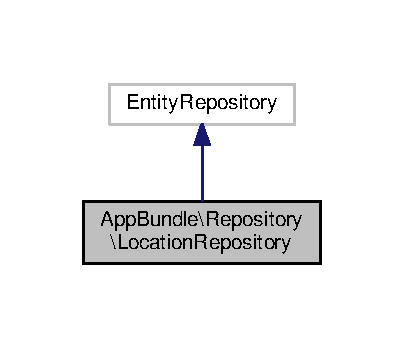
\includegraphics[width=194pt]{classAppBundle_1_1Repository_1_1LocationRepository__inherit__graph}
\end{center}
\end{figure}


Graphe de collaboration de App\+Bundle\textbackslash{}Repository\textbackslash{}Location\+Repository\+:\nopagebreak
\begin{figure}[H]
\begin{center}
\leavevmode
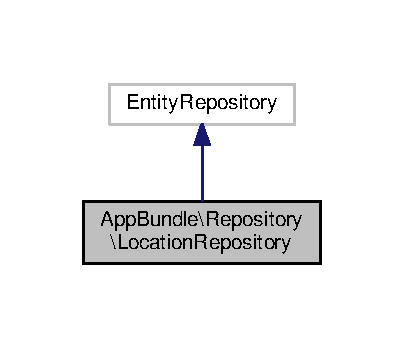
\includegraphics[width=194pt]{classAppBundle_1_1Repository_1_1LocationRepository__coll__graph}
\end{center}
\end{figure}


\subsection{Description détaillée}
\hyperlink{classAppBundle_1_1Repository_1_1LocationRepository}{Location\+Repository}

This class was generated by the \hyperlink{namespaceAppBundle_1_1Doctrine}{Doctrine} O\+RM. Add your own custom repository methods below. 

La documentation de cette classe a été générée à partir du fichier suivant \+:\begin{DoxyCompactItemize}
\item 
src/\+App\+Bundle/\+Repository/Location\+Repository.\+php\end{DoxyCompactItemize}

\hypertarget{classAppBundle_1_1Form_1_1LoginForm}{}\section{Référence de la classe App\+Bundle\textbackslash{}Form\textbackslash{}Login\+Form}
\label{classAppBundle_1_1Form_1_1LoginForm}\index{App\+Bundle\textbackslash{}\+Form\textbackslash{}\+Login\+Form@{App\+Bundle\textbackslash{}\+Form\textbackslash{}\+Login\+Form}}


Graphe d\textquotesingle{}héritage de App\+Bundle\textbackslash{}Form\textbackslash{}Login\+Form\+:\nopagebreak
\begin{figure}[H]
\begin{center}
\leavevmode
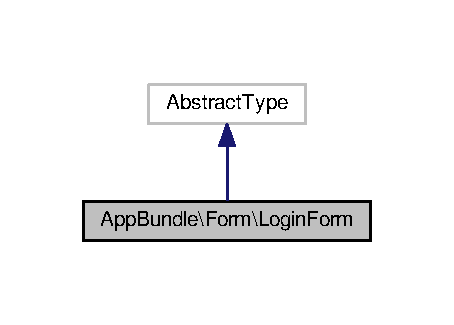
\includegraphics[width=218pt]{classAppBundle_1_1Form_1_1LoginForm__inherit__graph}
\end{center}
\end{figure}


Graphe de collaboration de App\+Bundle\textbackslash{}Form\textbackslash{}Login\+Form\+:\nopagebreak
\begin{figure}[H]
\begin{center}
\leavevmode
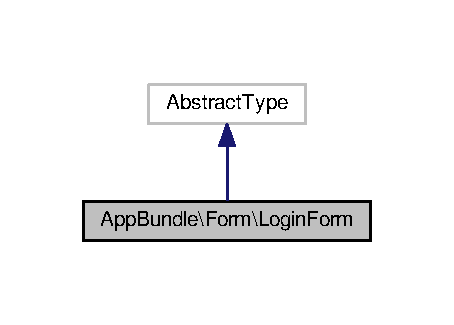
\includegraphics[width=218pt]{classAppBundle_1_1Form_1_1LoginForm__coll__graph}
\end{center}
\end{figure}
\subsection*{Fonctions membres publiques}
\begin{DoxyCompactItemize}
\item 
\mbox{\Hypertarget{classAppBundle_1_1Form_1_1LoginForm_a84f92c4eaab99ce9eb1361f5fa7e4091}\label{classAppBundle_1_1Form_1_1LoginForm_a84f92c4eaab99ce9eb1361f5fa7e4091}} 
{\bfseries build\+Form} (Form\+Builder\+Interface \$builder, array \$options)
\end{DoxyCompactItemize}


La documentation de cette classe a été générée à partir du fichier suivant \+:\begin{DoxyCompactItemize}
\item 
src/\+App\+Bundle/\+Form/Login\+Form.\+php\end{DoxyCompactItemize}

\hypertarget{classAppBundle_1_1Form_1_1NewEventForm}{}\section{Référence de la classe App\+Bundle\textbackslash{}Form\textbackslash{}New\+Event\+Form}
\label{classAppBundle_1_1Form_1_1NewEventForm}\index{App\+Bundle\textbackslash{}\+Form\textbackslash{}\+New\+Event\+Form@{App\+Bundle\textbackslash{}\+Form\textbackslash{}\+New\+Event\+Form}}


Graphe d\textquotesingle{}héritage de App\+Bundle\textbackslash{}Form\textbackslash{}New\+Event\+Form\+:\nopagebreak
\begin{figure}[H]
\begin{center}
\leavevmode
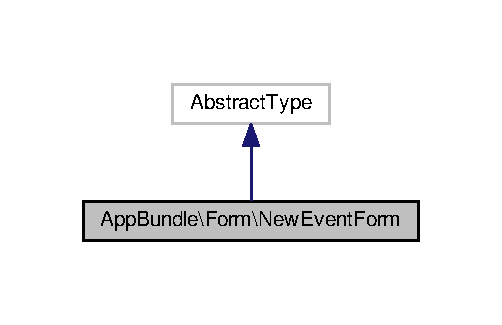
\includegraphics[width=241pt]{classAppBundle_1_1Form_1_1NewEventForm__inherit__graph}
\end{center}
\end{figure}


Graphe de collaboration de App\+Bundle\textbackslash{}Form\textbackslash{}New\+Event\+Form\+:\nopagebreak
\begin{figure}[H]
\begin{center}
\leavevmode
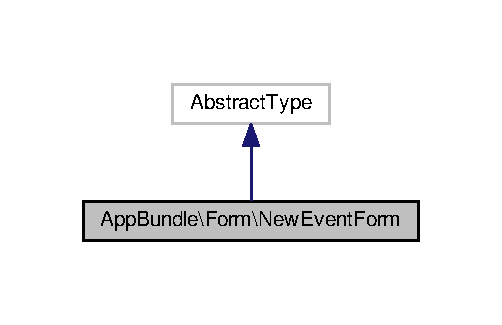
\includegraphics[width=241pt]{classAppBundle_1_1Form_1_1NewEventForm__coll__graph}
\end{center}
\end{figure}
\subsection*{Fonctions membres publiques}
\begin{DoxyCompactItemize}
\item 
\mbox{\Hypertarget{classAppBundle_1_1Form_1_1NewEventForm_a8cf71eb9f00d33293aafd4efa44982f5}\label{classAppBundle_1_1Form_1_1NewEventForm_a8cf71eb9f00d33293aafd4efa44982f5}} 
{\bfseries build\+Form} (Form\+Builder\+Interface \$builder, array \$options)
\item 
\mbox{\Hypertarget{classAppBundle_1_1Form_1_1NewEventForm_a862390c98e7a2f1fe7bc057329a83c46}\label{classAppBundle_1_1Form_1_1NewEventForm_a862390c98e7a2f1fe7bc057329a83c46}} 
{\bfseries configure\+Options} (Options\+Resolver \$resolver)
\end{DoxyCompactItemize}


La documentation de cette classe a été générée à partir du fichier suivant \+:\begin{DoxyCompactItemize}
\item 
src/\+App\+Bundle/\+Form/New\+Event\+Form.\+php\end{DoxyCompactItemize}

\hypertarget{classPhpIniRequirement}{}\section{Référence de la classe Php\+Ini\+Requirement}
\label{classPhpIniRequirement}\index{Php\+Ini\+Requirement@{Php\+Ini\+Requirement}}


Graphe d\textquotesingle{}héritage de Php\+Ini\+Requirement\+:\nopagebreak
\begin{figure}[H]
\begin{center}
\leavevmode
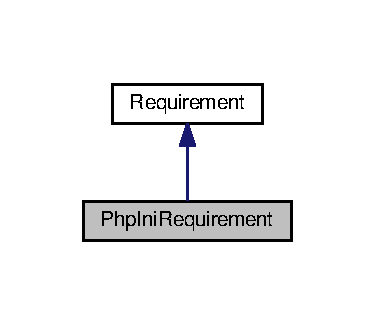
\includegraphics[width=180pt]{classPhpIniRequirement__inherit__graph}
\end{center}
\end{figure}


Graphe de collaboration de Php\+Ini\+Requirement\+:\nopagebreak
\begin{figure}[H]
\begin{center}
\leavevmode
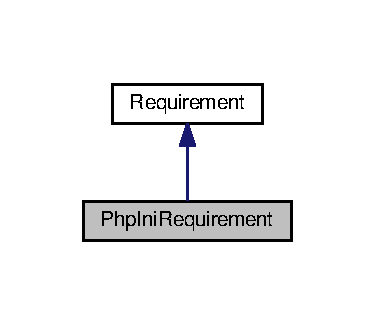
\includegraphics[width=180pt]{classPhpIniRequirement__coll__graph}
\end{center}
\end{figure}
\subsection*{Fonctions membres publiques}
\begin{DoxyCompactItemize}
\item 
\hyperlink{classPhpIniRequirement_af3e88e1bbec416c36ed54c88ca1397bb}{\+\_\+\+\_\+construct} (\$cfg\+Name, \$evaluation, \$approve\+Cfg\+Absence=false, \$test\+Message=null, \$help\+Html=null, \$help\+Text=null, \$optional=false)
\end{DoxyCompactItemize}


\subsection{Description détaillée}
Represents a P\+HP requirement in form of a php.\+ini configuration.

\begin{DoxyAuthor}{Auteur}
Tobias Schultze \href{http://tobion.de}{\tt http\+://tobion.\+de} 
\end{DoxyAuthor}


\subsection{Documentation des constructeurs et destructeur}
\mbox{\Hypertarget{classPhpIniRequirement_af3e88e1bbec416c36ed54c88ca1397bb}\label{classPhpIniRequirement_af3e88e1bbec416c36ed54c88ca1397bb}} 
\index{Php\+Ini\+Requirement@{Php\+Ini\+Requirement}!\+\_\+\+\_\+construct@{\+\_\+\+\_\+construct}}
\index{\+\_\+\+\_\+construct@{\+\_\+\+\_\+construct}!Php\+Ini\+Requirement@{Php\+Ini\+Requirement}}
\subsubsection{\texorpdfstring{\+\_\+\+\_\+construct()}{\_\_construct()}}
{\footnotesize\ttfamily Php\+Ini\+Requirement\+::\+\_\+\+\_\+construct (\begin{DoxyParamCaption}\item[{}]{\$cfg\+Name,  }\item[{}]{\$evaluation,  }\item[{}]{\$approve\+Cfg\+Absence = {\ttfamily false},  }\item[{}]{\$test\+Message = {\ttfamily null},  }\item[{}]{\$help\+Html = {\ttfamily null},  }\item[{}]{\$help\+Text = {\ttfamily null},  }\item[{}]{\$optional = {\ttfamily false} }\end{DoxyParamCaption})}

Constructor that initializes the requirement.


\begin{DoxyParams}[1]{Paramètres}
string & {\em \$cfg\+Name} & The configuration name used for ini\+\_\+get() \\
\hline
bool | callback & {\em \$evaluation} & Either a boolean indicating whether the configuration should evaluate to true or false, or a callback function receiving the configuration value as parameter to determine the fulfillment of the requirement \\
\hline
bool & {\em \$approve\+Cfg\+Absence} & If true the \hyperlink{classRequirement}{Requirement} will be fulfilled even if the configuration option does not exist, i.\+e. ini\+\_\+get() returns false. This is helpful for abandoned configs in later P\+HP versions or configs of an optional extension, like Suhosin. Example\+: You require a config to be true but P\+HP later removes this config and defaults it to true internally. \\
\hline
string | null & {\em \$test\+Message} & The message for testing the requirement (when null and \$evaluation is a boolean a default message is derived) \\
\hline
string | null & {\em \$help\+Html} & The help text formatted in H\+T\+ML for resolving the problem (when null and \$evaluation is a boolean a default help is derived) \\
\hline
string | null & {\em \$help\+Text} & The help text (when null, it will be inferred from \$help\+Html, i.\+e. stripped from H\+T\+ML tags) \\
\hline
bool & {\em \$optional} & Whether this is only an optional recommendation not a mandatory requirement \\
\hline
\end{DoxyParams}


La documentation de cette classe a été générée à partir du fichier suivant \+:\begin{DoxyCompactItemize}
\item 
var/Symfony\+Requirements.\+php\end{DoxyCompactItemize}

\hypertarget{classAppBundle_1_1Form_1_1ProfileEditForm}{}\section{Référence de la classe App\+Bundle\textbackslash{}Form\textbackslash{}Profile\+Edit\+Form}
\label{classAppBundle_1_1Form_1_1ProfileEditForm}\index{App\+Bundle\textbackslash{}\+Form\textbackslash{}\+Profile\+Edit\+Form@{App\+Bundle\textbackslash{}\+Form\textbackslash{}\+Profile\+Edit\+Form}}


Graphe d\textquotesingle{}héritage de App\+Bundle\textbackslash{}Form\textbackslash{}Profile\+Edit\+Form\+:\nopagebreak
\begin{figure}[H]
\begin{center}
\leavevmode
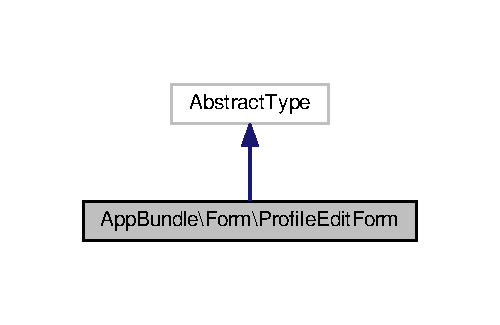
\includegraphics[width=240pt]{classAppBundle_1_1Form_1_1ProfileEditForm__inherit__graph}
\end{center}
\end{figure}


Graphe de collaboration de App\+Bundle\textbackslash{}Form\textbackslash{}Profile\+Edit\+Form\+:\nopagebreak
\begin{figure}[H]
\begin{center}
\leavevmode
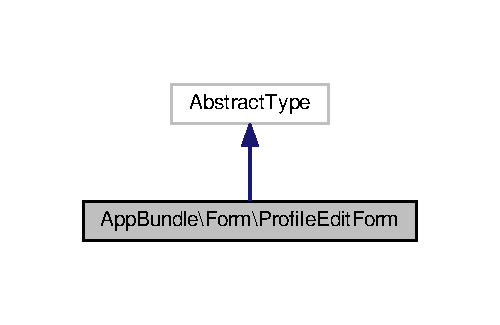
\includegraphics[width=240pt]{classAppBundle_1_1Form_1_1ProfileEditForm__coll__graph}
\end{center}
\end{figure}
\subsection*{Fonctions membres publiques}
\begin{DoxyCompactItemize}
\item 
\mbox{\Hypertarget{classAppBundle_1_1Form_1_1ProfileEditForm_a9f70142b9d4ddce69f60c49499040a01}\label{classAppBundle_1_1Form_1_1ProfileEditForm_a9f70142b9d4ddce69f60c49499040a01}} 
{\bfseries build\+Form} (Form\+Builder\+Interface \$builder, array \$options)
\item 
\mbox{\Hypertarget{classAppBundle_1_1Form_1_1ProfileEditForm_ab5aa7b78cf0f50661016c0afb3c81f88}\label{classAppBundle_1_1Form_1_1ProfileEditForm_ab5aa7b78cf0f50661016c0afb3c81f88}} 
{\bfseries configure\+Options} (Options\+Resolver \$resolver)
\end{DoxyCompactItemize}


La documentation de cette classe a été générée à partir du fichier suivant \+:\begin{DoxyCompactItemize}
\item 
src/\+App\+Bundle/\+Form/Profile\+Edit\+Form.\+php\end{DoxyCompactItemize}

\hypertarget{classAppBundle_1_1Form_1_1RegisterForm}{}\section{Référence de la classe App\+Bundle\textbackslash{}Form\textbackslash{}Register\+Form}
\label{classAppBundle_1_1Form_1_1RegisterForm}\index{App\+Bundle\textbackslash{}\+Form\textbackslash{}\+Register\+Form@{App\+Bundle\textbackslash{}\+Form\textbackslash{}\+Register\+Form}}


Graphe d\textquotesingle{}héritage de App\+Bundle\textbackslash{}Form\textbackslash{}Register\+Form\+:\nopagebreak
\begin{figure}[H]
\begin{center}
\leavevmode
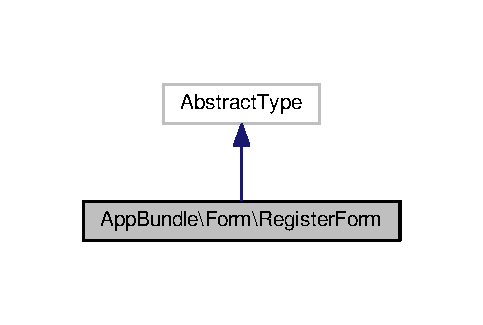
\includegraphics[width=232pt]{classAppBundle_1_1Form_1_1RegisterForm__inherit__graph}
\end{center}
\end{figure}


Graphe de collaboration de App\+Bundle\textbackslash{}Form\textbackslash{}Register\+Form\+:\nopagebreak
\begin{figure}[H]
\begin{center}
\leavevmode
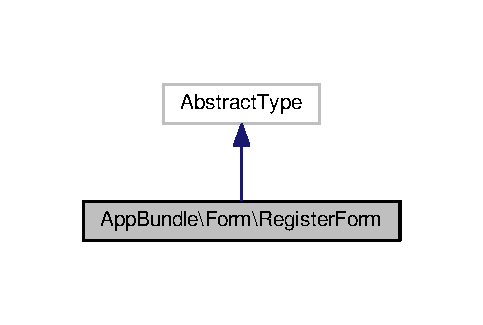
\includegraphics[width=232pt]{classAppBundle_1_1Form_1_1RegisterForm__coll__graph}
\end{center}
\end{figure}
\subsection*{Fonctions membres publiques}
\begin{DoxyCompactItemize}
\item 
\mbox{\Hypertarget{classAppBundle_1_1Form_1_1RegisterForm_a37d16fbd4a2a4841a010cc2e8e5edfd0}\label{classAppBundle_1_1Form_1_1RegisterForm_a37d16fbd4a2a4841a010cc2e8e5edfd0}} 
{\bfseries build\+Form} (Form\+Builder\+Interface \$builder, array \$options)
\item 
\mbox{\Hypertarget{classAppBundle_1_1Form_1_1RegisterForm_af00907a88d762aca1591808cc31f7778}\label{classAppBundle_1_1Form_1_1RegisterForm_af00907a88d762aca1591808cc31f7778}} 
{\bfseries configure\+Options} (Options\+Resolver \$resolver)
\end{DoxyCompactItemize}


La documentation de cette classe a été générée à partir du fichier suivant \+:\begin{DoxyCompactItemize}
\item 
src/\+App\+Bundle/\+Form/Register\+Form.\+php\end{DoxyCompactItemize}

\hypertarget{classRequirement}{}\section{Référence de la classe Requirement}
\label{classRequirement}\index{Requirement@{Requirement}}


Graphe d\textquotesingle{}héritage de Requirement\+:\nopagebreak
\begin{figure}[H]
\begin{center}
\leavevmode
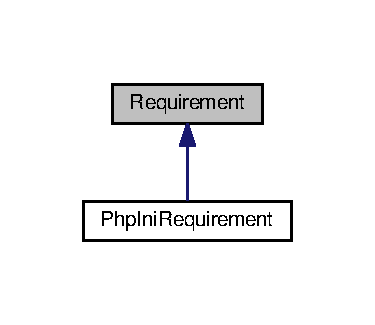
\includegraphics[width=180pt]{classRequirement__inherit__graph}
\end{center}
\end{figure}
\subsection*{Fonctions membres publiques}
\begin{DoxyCompactItemize}
\item 
\hyperlink{classRequirement_aed1695de1426aa5912a889bd93b66c83}{\+\_\+\+\_\+construct} (\$fulfilled, \$test\+Message, \$help\+Html, \$help\+Text=null, \$optional=false)
\item 
\hyperlink{classRequirement_aba605020ffa080b4d5b7217fc42822f0}{is\+Fulfilled} ()
\item 
\hyperlink{classRequirement_ac4cc7cb836c9e0c11018cef57a0fbc4d}{get\+Test\+Message} ()
\item 
\hyperlink{classRequirement_a6de91d308edfd46aada84b2faa16db01}{get\+Help\+Text} ()
\item 
\hyperlink{classRequirement_ad1ba7e3c3a6b1e94877d0d9ed66643dd}{get\+Help\+Html} ()
\item 
\hyperlink{classRequirement_a2e42f150791b2995f18048c7b21c7805}{is\+Optional} ()
\end{DoxyCompactItemize}


\subsection{Description détaillée}
Represents a single P\+HP requirement, e.\+g. an installed extension. It can be a mandatory requirement or an optional recommendation. There is a special subclass, named \hyperlink{classPhpIniRequirement}{Php\+Ini\+Requirement}, to check a php.\+ini configuration.

\begin{DoxyAuthor}{Auteur}
Tobias Schultze \href{http://tobion.de}{\tt http\+://tobion.\+de} 
\end{DoxyAuthor}


\subsection{Documentation des constructeurs et destructeur}
\mbox{\Hypertarget{classRequirement_aed1695de1426aa5912a889bd93b66c83}\label{classRequirement_aed1695de1426aa5912a889bd93b66c83}} 
\index{Requirement@{Requirement}!\+\_\+\+\_\+construct@{\+\_\+\+\_\+construct}}
\index{\+\_\+\+\_\+construct@{\+\_\+\+\_\+construct}!Requirement@{Requirement}}
\subsubsection{\texorpdfstring{\+\_\+\+\_\+construct()}{\_\_construct()}}
{\footnotesize\ttfamily Requirement\+::\+\_\+\+\_\+construct (\begin{DoxyParamCaption}\item[{}]{\$fulfilled,  }\item[{}]{\$test\+Message,  }\item[{}]{\$help\+Html,  }\item[{}]{\$help\+Text = {\ttfamily null},  }\item[{}]{\$optional = {\ttfamily false} }\end{DoxyParamCaption})}

Constructor that initializes the requirement.


\begin{DoxyParams}[1]{Paramètres}
bool & {\em \$fulfilled} & Whether the requirement is fulfilled \\
\hline
string & {\em \$test\+Message} & The message for testing the requirement \\
\hline
string & {\em \$help\+Html} & The help text formatted in H\+T\+ML for resolving the problem \\
\hline
string | null & {\em \$help\+Text} & The help text (when null, it will be inferred from \$help\+Html, i.\+e. stripped from H\+T\+ML tags) \\
\hline
bool & {\em \$optional} & Whether this is only an optional recommendation not a mandatory requirement \\
\hline
\end{DoxyParams}


\subsection{Documentation des fonctions membres}
\mbox{\Hypertarget{classRequirement_ad1ba7e3c3a6b1e94877d0d9ed66643dd}\label{classRequirement_ad1ba7e3c3a6b1e94877d0d9ed66643dd}} 
\index{Requirement@{Requirement}!get\+Help\+Html@{get\+Help\+Html}}
\index{get\+Help\+Html@{get\+Help\+Html}!Requirement@{Requirement}}
\subsubsection{\texorpdfstring{get\+Help\+Html()}{getHelpHtml()}}
{\footnotesize\ttfamily Requirement\+::get\+Help\+Html (\begin{DoxyParamCaption}{ }\end{DoxyParamCaption})}

Returns the help text formatted in H\+T\+ML.

\begin{DoxyReturn}{Renvoie}
string The H\+T\+ML help 
\end{DoxyReturn}
\mbox{\Hypertarget{classRequirement_a6de91d308edfd46aada84b2faa16db01}\label{classRequirement_a6de91d308edfd46aada84b2faa16db01}} 
\index{Requirement@{Requirement}!get\+Help\+Text@{get\+Help\+Text}}
\index{get\+Help\+Text@{get\+Help\+Text}!Requirement@{Requirement}}
\subsubsection{\texorpdfstring{get\+Help\+Text()}{getHelpText()}}
{\footnotesize\ttfamily Requirement\+::get\+Help\+Text (\begin{DoxyParamCaption}{ }\end{DoxyParamCaption})}

Returns the help text for resolving the problem.

\begin{DoxyReturn}{Renvoie}
string The help text 
\end{DoxyReturn}
\mbox{\Hypertarget{classRequirement_ac4cc7cb836c9e0c11018cef57a0fbc4d}\label{classRequirement_ac4cc7cb836c9e0c11018cef57a0fbc4d}} 
\index{Requirement@{Requirement}!get\+Test\+Message@{get\+Test\+Message}}
\index{get\+Test\+Message@{get\+Test\+Message}!Requirement@{Requirement}}
\subsubsection{\texorpdfstring{get\+Test\+Message()}{getTestMessage()}}
{\footnotesize\ttfamily Requirement\+::get\+Test\+Message (\begin{DoxyParamCaption}{ }\end{DoxyParamCaption})}

Returns the message for testing the requirement.

\begin{DoxyReturn}{Renvoie}
string The test message 
\end{DoxyReturn}
\mbox{\Hypertarget{classRequirement_aba605020ffa080b4d5b7217fc42822f0}\label{classRequirement_aba605020ffa080b4d5b7217fc42822f0}} 
\index{Requirement@{Requirement}!is\+Fulfilled@{is\+Fulfilled}}
\index{is\+Fulfilled@{is\+Fulfilled}!Requirement@{Requirement}}
\subsubsection{\texorpdfstring{is\+Fulfilled()}{isFulfilled()}}
{\footnotesize\ttfamily Requirement\+::is\+Fulfilled (\begin{DoxyParamCaption}{ }\end{DoxyParamCaption})}

Returns whether the requirement is fulfilled.

\begin{DoxyReturn}{Renvoie}
bool true if fulfilled, otherwise false 
\end{DoxyReturn}
\mbox{\Hypertarget{classRequirement_a2e42f150791b2995f18048c7b21c7805}\label{classRequirement_a2e42f150791b2995f18048c7b21c7805}} 
\index{Requirement@{Requirement}!is\+Optional@{is\+Optional}}
\index{is\+Optional@{is\+Optional}!Requirement@{Requirement}}
\subsubsection{\texorpdfstring{is\+Optional()}{isOptional()}}
{\footnotesize\ttfamily Requirement\+::is\+Optional (\begin{DoxyParamCaption}{ }\end{DoxyParamCaption})}

Returns whether this is only an optional recommendation and not a mandatory requirement.

\begin{DoxyReturn}{Renvoie}
bool true if optional, false if mandatory 
\end{DoxyReturn}


La documentation de cette classe a été générée à partir du fichier suivant \+:\begin{DoxyCompactItemize}
\item 
var/Symfony\+Requirements.\+php\end{DoxyCompactItemize}

\hypertarget{classRequirementCollection}{}\section{Référence de la classe Requirement\+Collection}
\label{classRequirementCollection}\index{Requirement\+Collection@{Requirement\+Collection}}


Graphe d\textquotesingle{}héritage de Requirement\+Collection\+:\nopagebreak
\begin{figure}[H]
\begin{center}
\leavevmode
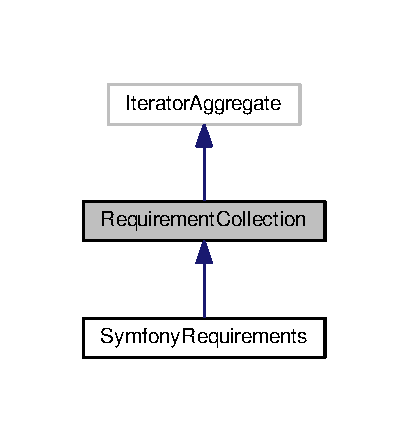
\includegraphics[width=196pt]{classRequirementCollection__inherit__graph}
\end{center}
\end{figure}


Graphe de collaboration de Requirement\+Collection\+:\nopagebreak
\begin{figure}[H]
\begin{center}
\leavevmode
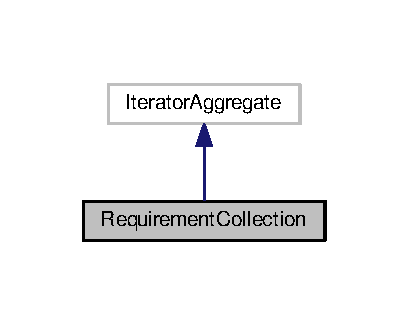
\includegraphics[width=196pt]{classRequirementCollection__coll__graph}
\end{center}
\end{figure}
\subsection*{Fonctions membres publiques}
\begin{DoxyCompactItemize}
\item 
\hyperlink{classRequirementCollection_a9b1922282e30ea8d9e267e206f63e071}{get\+Iterator} ()
\item 
\hyperlink{classRequirementCollection_a16be85daada80688601baf1d4048d4c6}{add} (\hyperlink{classRequirement}{Requirement} \$requirement)
\item 
\hyperlink{classRequirementCollection_a275b139b8f1daecf52952e67cb5bc6cf}{add\+Requirement} (\$fulfilled, \$test\+Message, \$help\+Html, \$help\+Text=null)
\item 
\hyperlink{classRequirementCollection_aa0c7a2d729d6a1d32d363b9c02d00b40}{add\+Recommendation} (\$fulfilled, \$test\+Message, \$help\+Html, \$help\+Text=null)
\item 
\hyperlink{classRequirementCollection_a21190a79cf3a13a6a4c9c7133c919d8f}{add\+Php\+Ini\+Requirement} (\$cfg\+Name, \$evaluation, \$approve\+Cfg\+Absence=false, \$test\+Message=null, \$help\+Html=null, \$help\+Text=null)
\item 
\hyperlink{classRequirementCollection_afeba77fa6ca369631f8a602800e9e29d}{add\+Php\+Ini\+Recommendation} (\$cfg\+Name, \$evaluation, \$approve\+Cfg\+Absence=false, \$test\+Message=null, \$help\+Html=null, \$help\+Text=null)
\item 
\hyperlink{classRequirementCollection_a4de7d0d4e50130610d6d6d3cadc5c91c}{add\+Collection} (\hyperlink{classRequirementCollection}{Requirement\+Collection} \$collection)
\item 
\hyperlink{classRequirementCollection_a7b84e71c211825222e548a5cc296f99b}{all} ()
\item 
\hyperlink{classRequirementCollection_a86ec2f872cec0395bc1f0206c2de8c6d}{get\+Requirements} ()
\item 
\hyperlink{classRequirementCollection_acd45245ad3ababfaeb5f0565add5e7cc}{get\+Failed\+Requirements} ()
\item 
\hyperlink{classRequirementCollection_aa21bc7027e02a0366c52227fbd3acb35}{get\+Recommendations} ()
\item 
\hyperlink{classRequirementCollection_ae11e0e7a5fd890a48f29d35876684e14}{get\+Failed\+Recommendations} ()
\item 
\hyperlink{classRequirementCollection_ae2b1f4fc39d0139dbebe0783cc100029}{has\+Php\+Ini\+Config\+Issue} ()
\item 
\hyperlink{classRequirementCollection_a40f0ae0bf0d5e4d0abcece27c151527d}{get\+Php\+Ini\+Config\+Path} ()
\end{DoxyCompactItemize}


\subsection{Description détaillée}
A \hyperlink{classRequirementCollection}{Requirement\+Collection} represents a set of \hyperlink{classRequirement}{Requirement} instances.

\begin{DoxyAuthor}{Auteur}
Tobias Schultze \href{http://tobion.de}{\tt http\+://tobion.\+de} 
\end{DoxyAuthor}


\subsection{Documentation des fonctions membres}
\mbox{\Hypertarget{classRequirementCollection_a16be85daada80688601baf1d4048d4c6}\label{classRequirementCollection_a16be85daada80688601baf1d4048d4c6}} 
\index{Requirement\+Collection@{Requirement\+Collection}!add@{add}}
\index{add@{add}!Requirement\+Collection@{Requirement\+Collection}}
\subsubsection{\texorpdfstring{add()}{add()}}
{\footnotesize\ttfamily Requirement\+Collection\+::add (\begin{DoxyParamCaption}\item[{\hyperlink{classRequirement}{Requirement}}]{\$requirement }\end{DoxyParamCaption})}

Adds a \hyperlink{classRequirement}{Requirement}.


\begin{DoxyParams}[1]{Paramètres}
\hyperlink{classRequirement}{Requirement} & {\em \$requirement} & A \hyperlink{classRequirement}{Requirement} instance \\
\hline
\end{DoxyParams}
\mbox{\Hypertarget{classRequirementCollection_a4de7d0d4e50130610d6d6d3cadc5c91c}\label{classRequirementCollection_a4de7d0d4e50130610d6d6d3cadc5c91c}} 
\index{Requirement\+Collection@{Requirement\+Collection}!add\+Collection@{add\+Collection}}
\index{add\+Collection@{add\+Collection}!Requirement\+Collection@{Requirement\+Collection}}
\subsubsection{\texorpdfstring{add\+Collection()}{addCollection()}}
{\footnotesize\ttfamily Requirement\+Collection\+::add\+Collection (\begin{DoxyParamCaption}\item[{\hyperlink{classRequirementCollection}{Requirement\+Collection}}]{\$collection }\end{DoxyParamCaption})}

Adds a requirement collection to the current set of requirements.


\begin{DoxyParams}[1]{Paramètres}
\hyperlink{classRequirementCollection}{Requirement\+Collection} & {\em \$collection} & A \hyperlink{classRequirementCollection}{Requirement\+Collection} instance \\
\hline
\end{DoxyParams}
\mbox{\Hypertarget{classRequirementCollection_afeba77fa6ca369631f8a602800e9e29d}\label{classRequirementCollection_afeba77fa6ca369631f8a602800e9e29d}} 
\index{Requirement\+Collection@{Requirement\+Collection}!add\+Php\+Ini\+Recommendation@{add\+Php\+Ini\+Recommendation}}
\index{add\+Php\+Ini\+Recommendation@{add\+Php\+Ini\+Recommendation}!Requirement\+Collection@{Requirement\+Collection}}
\subsubsection{\texorpdfstring{add\+Php\+Ini\+Recommendation()}{addPhpIniRecommendation()}}
{\footnotesize\ttfamily Requirement\+Collection\+::add\+Php\+Ini\+Recommendation (\begin{DoxyParamCaption}\item[{}]{\$cfg\+Name,  }\item[{}]{\$evaluation,  }\item[{}]{\$approve\+Cfg\+Absence = {\ttfamily false},  }\item[{}]{\$test\+Message = {\ttfamily null},  }\item[{}]{\$help\+Html = {\ttfamily null},  }\item[{}]{\$help\+Text = {\ttfamily null} }\end{DoxyParamCaption})}

Adds an optional recommendation in form of a php.\+ini configuration.


\begin{DoxyParams}[1]{Paramètres}
string & {\em \$cfg\+Name} & The configuration name used for ini\+\_\+get() \\
\hline
bool | callback & {\em \$evaluation} & Either a boolean indicating whether the configuration should evaluate to true or false, or a callback function receiving the configuration value as parameter to determine the fulfillment of the requirement \\
\hline
bool & {\em \$approve\+Cfg\+Absence} & If true the \hyperlink{classRequirement}{Requirement} will be fulfilled even if the configuration option does not exist, i.\+e. ini\+\_\+get() returns false. This is helpful for abandoned configs in later P\+HP versions or configs of an optional extension, like Suhosin. Example\+: You require a config to be true but P\+HP later removes this config and defaults it to true internally. \\
\hline
string & {\em \$test\+Message} & The message for testing the requirement (when null and \$evaluation is a boolean a default message is derived) \\
\hline
string & {\em \$help\+Html} & The help text formatted in H\+T\+ML for resolving the problem (when null and \$evaluation is a boolean a default help is derived) \\
\hline
string | null & {\em \$help\+Text} & The help text (when null, it will be inferred from \$help\+Html, i.\+e. stripped from H\+T\+ML tags) \\
\hline
\end{DoxyParams}
\mbox{\Hypertarget{classRequirementCollection_a21190a79cf3a13a6a4c9c7133c919d8f}\label{classRequirementCollection_a21190a79cf3a13a6a4c9c7133c919d8f}} 
\index{Requirement\+Collection@{Requirement\+Collection}!add\+Php\+Ini\+Requirement@{add\+Php\+Ini\+Requirement}}
\index{add\+Php\+Ini\+Requirement@{add\+Php\+Ini\+Requirement}!Requirement\+Collection@{Requirement\+Collection}}
\subsubsection{\texorpdfstring{add\+Php\+Ini\+Requirement()}{addPhpIniRequirement()}}
{\footnotesize\ttfamily Requirement\+Collection\+::add\+Php\+Ini\+Requirement (\begin{DoxyParamCaption}\item[{}]{\$cfg\+Name,  }\item[{}]{\$evaluation,  }\item[{}]{\$approve\+Cfg\+Absence = {\ttfamily false},  }\item[{}]{\$test\+Message = {\ttfamily null},  }\item[{}]{\$help\+Html = {\ttfamily null},  }\item[{}]{\$help\+Text = {\ttfamily null} }\end{DoxyParamCaption})}

Adds a mandatory requirement in form of a php.\+ini configuration.


\begin{DoxyParams}[1]{Paramètres}
string & {\em \$cfg\+Name} & The configuration name used for ini\+\_\+get() \\
\hline
bool | callback & {\em \$evaluation} & Either a boolean indicating whether the configuration should evaluate to true or false, or a callback function receiving the configuration value as parameter to determine the fulfillment of the requirement \\
\hline
bool & {\em \$approve\+Cfg\+Absence} & If true the \hyperlink{classRequirement}{Requirement} will be fulfilled even if the configuration option does not exist, i.\+e. ini\+\_\+get() returns false. This is helpful for abandoned configs in later P\+HP versions or configs of an optional extension, like Suhosin. Example\+: You require a config to be true but P\+HP later removes this config and defaults it to true internally. \\
\hline
string & {\em \$test\+Message} & The message for testing the requirement (when null and \$evaluation is a boolean a default message is derived) \\
\hline
string & {\em \$help\+Html} & The help text formatted in H\+T\+ML for resolving the problem (when null and \$evaluation is a boolean a default help is derived) \\
\hline
string | null & {\em \$help\+Text} & The help text (when null, it will be inferred from \$help\+Html, i.\+e. stripped from H\+T\+ML tags) \\
\hline
\end{DoxyParams}
\mbox{\Hypertarget{classRequirementCollection_aa0c7a2d729d6a1d32d363b9c02d00b40}\label{classRequirementCollection_aa0c7a2d729d6a1d32d363b9c02d00b40}} 
\index{Requirement\+Collection@{Requirement\+Collection}!add\+Recommendation@{add\+Recommendation}}
\index{add\+Recommendation@{add\+Recommendation}!Requirement\+Collection@{Requirement\+Collection}}
\subsubsection{\texorpdfstring{add\+Recommendation()}{addRecommendation()}}
{\footnotesize\ttfamily Requirement\+Collection\+::add\+Recommendation (\begin{DoxyParamCaption}\item[{}]{\$fulfilled,  }\item[{}]{\$test\+Message,  }\item[{}]{\$help\+Html,  }\item[{}]{\$help\+Text = {\ttfamily null} }\end{DoxyParamCaption})}

Adds an optional recommendation.


\begin{DoxyParams}[1]{Paramètres}
bool & {\em \$fulfilled} & Whether the recommendation is fulfilled \\
\hline
string & {\em \$test\+Message} & The message for testing the recommendation \\
\hline
string & {\em \$help\+Html} & The help text formatted in H\+T\+ML for resolving the problem \\
\hline
string | null & {\em \$help\+Text} & The help text (when null, it will be inferred from \$help\+Html, i.\+e. stripped from H\+T\+ML tags) \\
\hline
\end{DoxyParams}
\mbox{\Hypertarget{classRequirementCollection_a275b139b8f1daecf52952e67cb5bc6cf}\label{classRequirementCollection_a275b139b8f1daecf52952e67cb5bc6cf}} 
\index{Requirement\+Collection@{Requirement\+Collection}!add\+Requirement@{add\+Requirement}}
\index{add\+Requirement@{add\+Requirement}!Requirement\+Collection@{Requirement\+Collection}}
\subsubsection{\texorpdfstring{add\+Requirement()}{addRequirement()}}
{\footnotesize\ttfamily Requirement\+Collection\+::add\+Requirement (\begin{DoxyParamCaption}\item[{}]{\$fulfilled,  }\item[{}]{\$test\+Message,  }\item[{}]{\$help\+Html,  }\item[{}]{\$help\+Text = {\ttfamily null} }\end{DoxyParamCaption})}

Adds a mandatory requirement.


\begin{DoxyParams}[1]{Paramètres}
bool & {\em \$fulfilled} & Whether the requirement is fulfilled \\
\hline
string & {\em \$test\+Message} & The message for testing the requirement \\
\hline
string & {\em \$help\+Html} & The help text formatted in H\+T\+ML for resolving the problem \\
\hline
string | null & {\em \$help\+Text} & The help text (when null, it will be inferred from \$help\+Html, i.\+e. stripped from H\+T\+ML tags) \\
\hline
\end{DoxyParams}
\mbox{\Hypertarget{classRequirementCollection_a7b84e71c211825222e548a5cc296f99b}\label{classRequirementCollection_a7b84e71c211825222e548a5cc296f99b}} 
\index{Requirement\+Collection@{Requirement\+Collection}!all@{all}}
\index{all@{all}!Requirement\+Collection@{Requirement\+Collection}}
\subsubsection{\texorpdfstring{all()}{all()}}
{\footnotesize\ttfamily Requirement\+Collection\+::all (\begin{DoxyParamCaption}{ }\end{DoxyParamCaption})}

Returns both requirements and recommendations.

\begin{DoxyReturn}{Renvoie}
\hyperlink{classRequirement}{Requirement}\mbox{[}\mbox{]} 
\end{DoxyReturn}
\mbox{\Hypertarget{classRequirementCollection_ae11e0e7a5fd890a48f29d35876684e14}\label{classRequirementCollection_ae11e0e7a5fd890a48f29d35876684e14}} 
\index{Requirement\+Collection@{Requirement\+Collection}!get\+Failed\+Recommendations@{get\+Failed\+Recommendations}}
\index{get\+Failed\+Recommendations@{get\+Failed\+Recommendations}!Requirement\+Collection@{Requirement\+Collection}}
\subsubsection{\texorpdfstring{get\+Failed\+Recommendations()}{getFailedRecommendations()}}
{\footnotesize\ttfamily Requirement\+Collection\+::get\+Failed\+Recommendations (\begin{DoxyParamCaption}{ }\end{DoxyParamCaption})}

Returns the recommendations that were not met.

\begin{DoxyReturn}{Renvoie}
\hyperlink{classRequirement}{Requirement}\mbox{[}\mbox{]} 
\end{DoxyReturn}
\mbox{\Hypertarget{classRequirementCollection_acd45245ad3ababfaeb5f0565add5e7cc}\label{classRequirementCollection_acd45245ad3ababfaeb5f0565add5e7cc}} 
\index{Requirement\+Collection@{Requirement\+Collection}!get\+Failed\+Requirements@{get\+Failed\+Requirements}}
\index{get\+Failed\+Requirements@{get\+Failed\+Requirements}!Requirement\+Collection@{Requirement\+Collection}}
\subsubsection{\texorpdfstring{get\+Failed\+Requirements()}{getFailedRequirements()}}
{\footnotesize\ttfamily Requirement\+Collection\+::get\+Failed\+Requirements (\begin{DoxyParamCaption}{ }\end{DoxyParamCaption})}

Returns the mandatory requirements that were not met.

\begin{DoxyReturn}{Renvoie}
\hyperlink{classRequirement}{Requirement}\mbox{[}\mbox{]} 
\end{DoxyReturn}
\mbox{\Hypertarget{classRequirementCollection_a9b1922282e30ea8d9e267e206f63e071}\label{classRequirementCollection_a9b1922282e30ea8d9e267e206f63e071}} 
\index{Requirement\+Collection@{Requirement\+Collection}!get\+Iterator@{get\+Iterator}}
\index{get\+Iterator@{get\+Iterator}!Requirement\+Collection@{Requirement\+Collection}}
\subsubsection{\texorpdfstring{get\+Iterator()}{getIterator()}}
{\footnotesize\ttfamily Requirement\+Collection\+::get\+Iterator (\begin{DoxyParamCaption}{ }\end{DoxyParamCaption})}

Gets the current \hyperlink{classRequirementCollection}{Requirement\+Collection} as an Iterator.

\begin{DoxyReturn}{Renvoie}
Traversable A Traversable interface 
\end{DoxyReturn}
\mbox{\Hypertarget{classRequirementCollection_a40f0ae0bf0d5e4d0abcece27c151527d}\label{classRequirementCollection_a40f0ae0bf0d5e4d0abcece27c151527d}} 
\index{Requirement\+Collection@{Requirement\+Collection}!get\+Php\+Ini\+Config\+Path@{get\+Php\+Ini\+Config\+Path}}
\index{get\+Php\+Ini\+Config\+Path@{get\+Php\+Ini\+Config\+Path}!Requirement\+Collection@{Requirement\+Collection}}
\subsubsection{\texorpdfstring{get\+Php\+Ini\+Config\+Path()}{getPhpIniConfigPath()}}
{\footnotesize\ttfamily Requirement\+Collection\+::get\+Php\+Ini\+Config\+Path (\begin{DoxyParamCaption}{ }\end{DoxyParamCaption})}

Returns the P\+HP configuration file (php.\+ini) path.

\begin{DoxyReturn}{Renvoie}
string$\vert$false php.\+ini file path 
\end{DoxyReturn}
\mbox{\Hypertarget{classRequirementCollection_aa21bc7027e02a0366c52227fbd3acb35}\label{classRequirementCollection_aa21bc7027e02a0366c52227fbd3acb35}} 
\index{Requirement\+Collection@{Requirement\+Collection}!get\+Recommendations@{get\+Recommendations}}
\index{get\+Recommendations@{get\+Recommendations}!Requirement\+Collection@{Requirement\+Collection}}
\subsubsection{\texorpdfstring{get\+Recommendations()}{getRecommendations()}}
{\footnotesize\ttfamily Requirement\+Collection\+::get\+Recommendations (\begin{DoxyParamCaption}{ }\end{DoxyParamCaption})}

Returns all optional recommendations.

\begin{DoxyReturn}{Renvoie}
\hyperlink{classRequirement}{Requirement}\mbox{[}\mbox{]} 
\end{DoxyReturn}
\mbox{\Hypertarget{classRequirementCollection_a86ec2f872cec0395bc1f0206c2de8c6d}\label{classRequirementCollection_a86ec2f872cec0395bc1f0206c2de8c6d}} 
\index{Requirement\+Collection@{Requirement\+Collection}!get\+Requirements@{get\+Requirements}}
\index{get\+Requirements@{get\+Requirements}!Requirement\+Collection@{Requirement\+Collection}}
\subsubsection{\texorpdfstring{get\+Requirements()}{getRequirements()}}
{\footnotesize\ttfamily Requirement\+Collection\+::get\+Requirements (\begin{DoxyParamCaption}{ }\end{DoxyParamCaption})}

Returns all mandatory requirements.

\begin{DoxyReturn}{Renvoie}
\hyperlink{classRequirement}{Requirement}\mbox{[}\mbox{]} 
\end{DoxyReturn}
\mbox{\Hypertarget{classRequirementCollection_ae2b1f4fc39d0139dbebe0783cc100029}\label{classRequirementCollection_ae2b1f4fc39d0139dbebe0783cc100029}} 
\index{Requirement\+Collection@{Requirement\+Collection}!has\+Php\+Ini\+Config\+Issue@{has\+Php\+Ini\+Config\+Issue}}
\index{has\+Php\+Ini\+Config\+Issue@{has\+Php\+Ini\+Config\+Issue}!Requirement\+Collection@{Requirement\+Collection}}
\subsubsection{\texorpdfstring{has\+Php\+Ini\+Config\+Issue()}{hasPhpIniConfigIssue()}}
{\footnotesize\ttfamily Requirement\+Collection\+::has\+Php\+Ini\+Config\+Issue (\begin{DoxyParamCaption}{ }\end{DoxyParamCaption})}

Returns whether a php.\+ini configuration is not correct.

\begin{DoxyReturn}{Renvoie}
bool php.\+ini configuration problem? 
\end{DoxyReturn}


La documentation de cette classe a été générée à partir du fichier suivant \+:\begin{DoxyCompactItemize}
\item 
var/Symfony\+Requirements.\+php\end{DoxyCompactItemize}

\hypertarget{classAppBundle_1_1Entity_1_1Review}{}\section{Référence de la classe App\+Bundle\textbackslash{}Entity\textbackslash{}Review}
\label{classAppBundle_1_1Entity_1_1Review}\index{App\+Bundle\textbackslash{}\+Entity\textbackslash{}\+Review@{App\+Bundle\textbackslash{}\+Entity\textbackslash{}\+Review}}
\subsection*{Fonctions membres publiques}
\begin{DoxyCompactItemize}
\item 
\hyperlink{classAppBundle_1_1Entity_1_1Review_a7831df4f53b9e884952db1d4bf1fff0c}{get\+Id} ()
\item 
\hyperlink{classAppBundle_1_1Entity_1_1Review_abb860d7311313005a3d43c7ae4f5028f}{set\+Comment} (\$comment)
\item 
\hyperlink{classAppBundle_1_1Entity_1_1Review_afcf5bbea14b6c5ab6c4176626c71351c}{get\+Comment} ()
\item 
\hyperlink{classAppBundle_1_1Entity_1_1Review_a80b99fea75d03bb7beb8abf6ed842aac}{set\+Is\+Positive} (\$is\+Positive)
\item 
\hyperlink{classAppBundle_1_1Entity_1_1Review_a731b3c2e477ff4c22d5e96c628299c7a}{get\+Is\+Positive} ()
\item 
\hyperlink{classAppBundle_1_1Entity_1_1Review_a86f0645495f1ca5aab85cfb2e2f4782b}{set\+Author} (\textbackslash{}\hyperlink{classAppBundle_1_1Entity_1_1User}{App\+Bundle\textbackslash{}\+Entity\textbackslash{}\+User} \$author)
\item 
\hyperlink{classAppBundle_1_1Entity_1_1Review_a4cd28ac8bbe58dfc98e5a65b04235d88}{get\+Author} ()
\item 
\hyperlink{classAppBundle_1_1Entity_1_1Review_a1f01ea851e2dd32bd7e4fd6d5da2657e}{set\+Location} (\textbackslash{}\hyperlink{classAppBundle_1_1Entity_1_1Location}{App\+Bundle\textbackslash{}\+Entity\textbackslash{}\+Location} \$location)
\item 
\hyperlink{classAppBundle_1_1Entity_1_1Review_a0e43af27c5317baf107c021dce387388}{get\+Location} ()
\item 
\hyperlink{classAppBundle_1_1Entity_1_1Review_a41be2d79098867b4f7cab2cac880ca5c}{set\+Creation\+Date} (\$creation\+Date)
\item 
\hyperlink{classAppBundle_1_1Entity_1_1Review_af74135765b0b130f9b1a65f5242631b4}{get\+Creation\+Date} ()
\end{DoxyCompactItemize}


\subsection{Description détaillée}
\hyperlink{classAppBundle_1_1Entity_1_1Review}{Review}

(name=\char`\"{}review\char`\"{}) (repository\+Class=\char`\"{}\+App\+Bundle\textbackslash{}\+Repository\textbackslash{}\+Review\+Repository\char`\"{}) 

\subsection{Documentation des fonctions membres}
\mbox{\Hypertarget{classAppBundle_1_1Entity_1_1Review_a4cd28ac8bbe58dfc98e5a65b04235d88}\label{classAppBundle_1_1Entity_1_1Review_a4cd28ac8bbe58dfc98e5a65b04235d88}} 
\index{App\+Bundle\+::\+Entity\+::\+Review@{App\+Bundle\+::\+Entity\+::\+Review}!get\+Author@{get\+Author}}
\index{get\+Author@{get\+Author}!App\+Bundle\+::\+Entity\+::\+Review@{App\+Bundle\+::\+Entity\+::\+Review}}
\subsubsection{\texorpdfstring{get\+Author()}{getAuthor()}}
{\footnotesize\ttfamily App\+Bundle\textbackslash{}\+Entity\textbackslash{}\+Review\+::get\+Author (\begin{DoxyParamCaption}{ }\end{DoxyParamCaption})}

Get author

\begin{DoxyReturn}{Renvoie}

\end{DoxyReturn}
\mbox{\Hypertarget{classAppBundle_1_1Entity_1_1Review_afcf5bbea14b6c5ab6c4176626c71351c}\label{classAppBundle_1_1Entity_1_1Review_afcf5bbea14b6c5ab6c4176626c71351c}} 
\index{App\+Bundle\+::\+Entity\+::\+Review@{App\+Bundle\+::\+Entity\+::\+Review}!get\+Comment@{get\+Comment}}
\index{get\+Comment@{get\+Comment}!App\+Bundle\+::\+Entity\+::\+Review@{App\+Bundle\+::\+Entity\+::\+Review}}
\subsubsection{\texorpdfstring{get\+Comment()}{getComment()}}
{\footnotesize\ttfamily App\+Bundle\textbackslash{}\+Entity\textbackslash{}\+Review\+::get\+Comment (\begin{DoxyParamCaption}{ }\end{DoxyParamCaption})}

Get comment

\begin{DoxyReturn}{Renvoie}
string 
\end{DoxyReturn}
\mbox{\Hypertarget{classAppBundle_1_1Entity_1_1Review_af74135765b0b130f9b1a65f5242631b4}\label{classAppBundle_1_1Entity_1_1Review_af74135765b0b130f9b1a65f5242631b4}} 
\index{App\+Bundle\+::\+Entity\+::\+Review@{App\+Bundle\+::\+Entity\+::\+Review}!get\+Creation\+Date@{get\+Creation\+Date}}
\index{get\+Creation\+Date@{get\+Creation\+Date}!App\+Bundle\+::\+Entity\+::\+Review@{App\+Bundle\+::\+Entity\+::\+Review}}
\subsubsection{\texorpdfstring{get\+Creation\+Date()}{getCreationDate()}}
{\footnotesize\ttfamily App\+Bundle\textbackslash{}\+Entity\textbackslash{}\+Review\+::get\+Creation\+Date (\begin{DoxyParamCaption}{ }\end{DoxyParamCaption})}

Get creation\+Date

\begin{DoxyReturn}{Renvoie}

\end{DoxyReturn}
\mbox{\Hypertarget{classAppBundle_1_1Entity_1_1Review_a7831df4f53b9e884952db1d4bf1fff0c}\label{classAppBundle_1_1Entity_1_1Review_a7831df4f53b9e884952db1d4bf1fff0c}} 
\index{App\+Bundle\+::\+Entity\+::\+Review@{App\+Bundle\+::\+Entity\+::\+Review}!get\+Id@{get\+Id}}
\index{get\+Id@{get\+Id}!App\+Bundle\+::\+Entity\+::\+Review@{App\+Bundle\+::\+Entity\+::\+Review}}
\subsubsection{\texorpdfstring{get\+Id()}{getId()}}
{\footnotesize\ttfamily App\+Bundle\textbackslash{}\+Entity\textbackslash{}\+Review\+::get\+Id (\begin{DoxyParamCaption}{ }\end{DoxyParamCaption})}

Get id

\begin{DoxyReturn}{Renvoie}
int 
\end{DoxyReturn}
\mbox{\Hypertarget{classAppBundle_1_1Entity_1_1Review_a731b3c2e477ff4c22d5e96c628299c7a}\label{classAppBundle_1_1Entity_1_1Review_a731b3c2e477ff4c22d5e96c628299c7a}} 
\index{App\+Bundle\+::\+Entity\+::\+Review@{App\+Bundle\+::\+Entity\+::\+Review}!get\+Is\+Positive@{get\+Is\+Positive}}
\index{get\+Is\+Positive@{get\+Is\+Positive}!App\+Bundle\+::\+Entity\+::\+Review@{App\+Bundle\+::\+Entity\+::\+Review}}
\subsubsection{\texorpdfstring{get\+Is\+Positive()}{getIsPositive()}}
{\footnotesize\ttfamily App\+Bundle\textbackslash{}\+Entity\textbackslash{}\+Review\+::get\+Is\+Positive (\begin{DoxyParamCaption}{ }\end{DoxyParamCaption})}

Get is\+Positive

\begin{DoxyReturn}{Renvoie}
bool 
\end{DoxyReturn}
\mbox{\Hypertarget{classAppBundle_1_1Entity_1_1Review_a0e43af27c5317baf107c021dce387388}\label{classAppBundle_1_1Entity_1_1Review_a0e43af27c5317baf107c021dce387388}} 
\index{App\+Bundle\+::\+Entity\+::\+Review@{App\+Bundle\+::\+Entity\+::\+Review}!get\+Location@{get\+Location}}
\index{get\+Location@{get\+Location}!App\+Bundle\+::\+Entity\+::\+Review@{App\+Bundle\+::\+Entity\+::\+Review}}
\subsubsection{\texorpdfstring{get\+Location()}{getLocation()}}
{\footnotesize\ttfamily App\+Bundle\textbackslash{}\+Entity\textbackslash{}\+Review\+::get\+Location (\begin{DoxyParamCaption}{ }\end{DoxyParamCaption})}

Get location

\begin{DoxyReturn}{Renvoie}

\end{DoxyReturn}
\mbox{\Hypertarget{classAppBundle_1_1Entity_1_1Review_a86f0645495f1ca5aab85cfb2e2f4782b}\label{classAppBundle_1_1Entity_1_1Review_a86f0645495f1ca5aab85cfb2e2f4782b}} 
\index{App\+Bundle\+::\+Entity\+::\+Review@{App\+Bundle\+::\+Entity\+::\+Review}!set\+Author@{set\+Author}}
\index{set\+Author@{set\+Author}!App\+Bundle\+::\+Entity\+::\+Review@{App\+Bundle\+::\+Entity\+::\+Review}}
\subsubsection{\texorpdfstring{set\+Author()}{setAuthor()}}
{\footnotesize\ttfamily App\+Bundle\textbackslash{}\+Entity\textbackslash{}\+Review\+::set\+Author (\begin{DoxyParamCaption}\item[{\textbackslash{}\hyperlink{classAppBundle_1_1Entity_1_1User}{App\+Bundle\textbackslash{}\+Entity\textbackslash{}\+User}}]{\$author }\end{DoxyParamCaption})}

Set author


\begin{DoxyParams}[1]{Paramètres}
\textbackslash{}\+App\+Bundle\textbackslash{}\+Entity\textbackslash{}\+User & {\em \$author} & \\
\hline
\end{DoxyParams}
\begin{DoxyReturn}{Renvoie}
\hyperlink{classAppBundle_1_1Entity_1_1Review}{Review} 
\end{DoxyReturn}
\mbox{\Hypertarget{classAppBundle_1_1Entity_1_1Review_abb860d7311313005a3d43c7ae4f5028f}\label{classAppBundle_1_1Entity_1_1Review_abb860d7311313005a3d43c7ae4f5028f}} 
\index{App\+Bundle\+::\+Entity\+::\+Review@{App\+Bundle\+::\+Entity\+::\+Review}!set\+Comment@{set\+Comment}}
\index{set\+Comment@{set\+Comment}!App\+Bundle\+::\+Entity\+::\+Review@{App\+Bundle\+::\+Entity\+::\+Review}}
\subsubsection{\texorpdfstring{set\+Comment()}{setComment()}}
{\footnotesize\ttfamily App\+Bundle\textbackslash{}\+Entity\textbackslash{}\+Review\+::set\+Comment (\begin{DoxyParamCaption}\item[{}]{\$comment }\end{DoxyParamCaption})}

Set comment


\begin{DoxyParams}[1]{Paramètres}
string & {\em \$comment} & \\
\hline
\end{DoxyParams}
\begin{DoxyReturn}{Renvoie}
\hyperlink{classAppBundle_1_1Entity_1_1Review}{Review} 
\end{DoxyReturn}
\mbox{\Hypertarget{classAppBundle_1_1Entity_1_1Review_a41be2d79098867b4f7cab2cac880ca5c}\label{classAppBundle_1_1Entity_1_1Review_a41be2d79098867b4f7cab2cac880ca5c}} 
\index{App\+Bundle\+::\+Entity\+::\+Review@{App\+Bundle\+::\+Entity\+::\+Review}!set\+Creation\+Date@{set\+Creation\+Date}}
\index{set\+Creation\+Date@{set\+Creation\+Date}!App\+Bundle\+::\+Entity\+::\+Review@{App\+Bundle\+::\+Entity\+::\+Review}}
\subsubsection{\texorpdfstring{set\+Creation\+Date()}{setCreationDate()}}
{\footnotesize\ttfamily App\+Bundle\textbackslash{}\+Entity\textbackslash{}\+Review\+::set\+Creation\+Date (\begin{DoxyParamCaption}\item[{}]{\$creation\+Date }\end{DoxyParamCaption})}

Set creation\+Date


\begin{DoxyParams}[1]{Paramètres}
\textbackslash{}\+Date\+Time & {\em \$creation\+Date} & \\
\hline
\end{DoxyParams}
\begin{DoxyReturn}{Renvoie}
\hyperlink{classAppBundle_1_1Entity_1_1Review}{Review} 
\end{DoxyReturn}
\mbox{\Hypertarget{classAppBundle_1_1Entity_1_1Review_a80b99fea75d03bb7beb8abf6ed842aac}\label{classAppBundle_1_1Entity_1_1Review_a80b99fea75d03bb7beb8abf6ed842aac}} 
\index{App\+Bundle\+::\+Entity\+::\+Review@{App\+Bundle\+::\+Entity\+::\+Review}!set\+Is\+Positive@{set\+Is\+Positive}}
\index{set\+Is\+Positive@{set\+Is\+Positive}!App\+Bundle\+::\+Entity\+::\+Review@{App\+Bundle\+::\+Entity\+::\+Review}}
\subsubsection{\texorpdfstring{set\+Is\+Positive()}{setIsPositive()}}
{\footnotesize\ttfamily App\+Bundle\textbackslash{}\+Entity\textbackslash{}\+Review\+::set\+Is\+Positive (\begin{DoxyParamCaption}\item[{}]{\$is\+Positive }\end{DoxyParamCaption})}

Set is\+Positive


\begin{DoxyParams}[1]{Paramètres}
boolean & {\em \$is\+Positive} & \\
\hline
\end{DoxyParams}
\begin{DoxyReturn}{Renvoie}
\hyperlink{classAppBundle_1_1Entity_1_1Review}{Review} 
\end{DoxyReturn}
\mbox{\Hypertarget{classAppBundle_1_1Entity_1_1Review_a1f01ea851e2dd32bd7e4fd6d5da2657e}\label{classAppBundle_1_1Entity_1_1Review_a1f01ea851e2dd32bd7e4fd6d5da2657e}} 
\index{App\+Bundle\+::\+Entity\+::\+Review@{App\+Bundle\+::\+Entity\+::\+Review}!set\+Location@{set\+Location}}
\index{set\+Location@{set\+Location}!App\+Bundle\+::\+Entity\+::\+Review@{App\+Bundle\+::\+Entity\+::\+Review}}
\subsubsection{\texorpdfstring{set\+Location()}{setLocation()}}
{\footnotesize\ttfamily App\+Bundle\textbackslash{}\+Entity\textbackslash{}\+Review\+::set\+Location (\begin{DoxyParamCaption}\item[{\textbackslash{}\hyperlink{classAppBundle_1_1Entity_1_1Location}{App\+Bundle\textbackslash{}\+Entity\textbackslash{}\+Location}}]{\$location }\end{DoxyParamCaption})}

Set location


\begin{DoxyParams}[1]{Paramètres}
\textbackslash{}\+App\+Bundle\textbackslash{}\+Entity\textbackslash{}\+Location & {\em \$location} & \\
\hline
\end{DoxyParams}
\begin{DoxyReturn}{Renvoie}
\hyperlink{classAppBundle_1_1Entity_1_1Review}{Review} 
\end{DoxyReturn}


La documentation de cette classe a été générée à partir du fichier suivant \+:\begin{DoxyCompactItemize}
\item 
src/\+App\+Bundle/\+Entity/Review.\+php\end{DoxyCompactItemize}

\hypertarget{classAppBundle_1_1Controller_1_1ReviewController}{}\section{Référence de la classe App\+Bundle\textbackslash{}Controller\textbackslash{}Review\+Controller}
\label{classAppBundle_1_1Controller_1_1ReviewController}\index{App\+Bundle\textbackslash{}\+Controller\textbackslash{}\+Review\+Controller@{App\+Bundle\textbackslash{}\+Controller\textbackslash{}\+Review\+Controller}}


Graphe d\textquotesingle{}héritage de App\+Bundle\textbackslash{}Controller\textbackslash{}Review\+Controller\+:\nopagebreak
\begin{figure}[H]
\begin{center}
\leavevmode
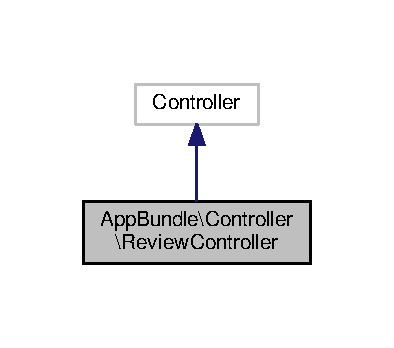
\includegraphics[width=189pt]{classAppBundle_1_1Controller_1_1ReviewController__inherit__graph}
\end{center}
\end{figure}


Graphe de collaboration de App\+Bundle\textbackslash{}Controller\textbackslash{}Review\+Controller\+:\nopagebreak
\begin{figure}[H]
\begin{center}
\leavevmode
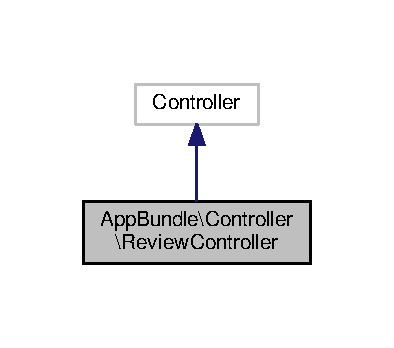
\includegraphics[width=189pt]{classAppBundle_1_1Controller_1_1ReviewController__coll__graph}
\end{center}
\end{figure}
\subsection*{Fonctions membres publiques}
\begin{DoxyCompactItemize}
\item 
\hyperlink{classAppBundle_1_1Controller_1_1ReviewController_aba2cab0f0fd4487f06d7d6ef205dd180}{index\+Action} (Request \$request, \$id)
\item 
\hyperlink{classAppBundle_1_1Controller_1_1ReviewController_a89fed73758d24e32060c68df209be415}{find\+Location\+From\+Map\+Id\+Action} (Request \$request, \$map\+Id, \$name, \$lat, \$lng)
\item 
\hyperlink{classAppBundle_1_1Controller_1_1ReviewController_ae9b55e90d1d07e4340a300253332f74c}{create\+Review\+Action} (Request \$request, \$id)
\item 
\hyperlink{classAppBundle_1_1Controller_1_1ReviewController_a71abcb3f902f7863f76b0ef4fea14dc3}{remove\+Review\+Action} (Request \$request, \$id)
\end{DoxyCompactItemize}


\subsection{Documentation des fonctions membres}
\mbox{\Hypertarget{classAppBundle_1_1Controller_1_1ReviewController_ae9b55e90d1d07e4340a300253332f74c}\label{classAppBundle_1_1Controller_1_1ReviewController_ae9b55e90d1d07e4340a300253332f74c}} 
\index{App\+Bundle\+::\+Controller\+::\+Review\+Controller@{App\+Bundle\+::\+Controller\+::\+Review\+Controller}!create\+Review\+Action@{create\+Review\+Action}}
\index{create\+Review\+Action@{create\+Review\+Action}!App\+Bundle\+::\+Controller\+::\+Review\+Controller@{App\+Bundle\+::\+Controller\+::\+Review\+Controller}}
\subsubsection{\texorpdfstring{create\+Review\+Action()}{createReviewAction()}}
{\footnotesize\ttfamily App\+Bundle\textbackslash{}\+Controller\textbackslash{}\+Review\+Controller\+::create\+Review\+Action (\begin{DoxyParamCaption}\item[{Request}]{\$request,  }\item[{}]{\$id }\end{DoxyParamCaption})}


\begin{DoxyParams}[1]{Paramètres}
Request & {\em \$request} & \\
\hline
 & {\em \$id} & \\
\hline
\end{DoxyParams}
\begin{DoxyReturn}{Renvoie}
$\vert$ (\char`\"{}/new/\{id\}\char`\"{}, name=\char`\"{}reviews-\/new\char`\"{}) 
\end{DoxyReturn}
\mbox{\Hypertarget{classAppBundle_1_1Controller_1_1ReviewController_a89fed73758d24e32060c68df209be415}\label{classAppBundle_1_1Controller_1_1ReviewController_a89fed73758d24e32060c68df209be415}} 
\index{App\+Bundle\+::\+Controller\+::\+Review\+Controller@{App\+Bundle\+::\+Controller\+::\+Review\+Controller}!find\+Location\+From\+Map\+Id\+Action@{find\+Location\+From\+Map\+Id\+Action}}
\index{find\+Location\+From\+Map\+Id\+Action@{find\+Location\+From\+Map\+Id\+Action}!App\+Bundle\+::\+Controller\+::\+Review\+Controller@{App\+Bundle\+::\+Controller\+::\+Review\+Controller}}
\subsubsection{\texorpdfstring{find\+Location\+From\+Map\+Id\+Action()}{findLocationFromMapIdAction()}}
{\footnotesize\ttfamily App\+Bundle\textbackslash{}\+Controller\textbackslash{}\+Review\+Controller\+::find\+Location\+From\+Map\+Id\+Action (\begin{DoxyParamCaption}\item[{Request}]{\$request,  }\item[{}]{\$map\+Id,  }\item[{}]{\$name,  }\item[{}]{\$lat,  }\item[{}]{\$lng }\end{DoxyParamCaption})}


\begin{DoxyParams}[1]{Paramètres}
Request & {\em \$request} & \\
\hline
 & {\em \$map\+Id} & \\
\hline
\end{DoxyParams}
\begin{DoxyReturn}{Renvoie}
(\char`\"{}/map\+Id/\{map\+Id\}/\{name\}/\{lat\}/\{lng\}\char`\"{}, name=\char`\"{}reviews-\/mapid-\/finder\char`\"{}, options=\{\char`\"{}expose\char`\"{} = true\}) 
\end{DoxyReturn}
\mbox{\Hypertarget{classAppBundle_1_1Controller_1_1ReviewController_aba2cab0f0fd4487f06d7d6ef205dd180}\label{classAppBundle_1_1Controller_1_1ReviewController_aba2cab0f0fd4487f06d7d6ef205dd180}} 
\index{App\+Bundle\+::\+Controller\+::\+Review\+Controller@{App\+Bundle\+::\+Controller\+::\+Review\+Controller}!index\+Action@{index\+Action}}
\index{index\+Action@{index\+Action}!App\+Bundle\+::\+Controller\+::\+Review\+Controller@{App\+Bundle\+::\+Controller\+::\+Review\+Controller}}
\subsubsection{\texorpdfstring{index\+Action()}{indexAction()}}
{\footnotesize\ttfamily App\+Bundle\textbackslash{}\+Controller\textbackslash{}\+Review\+Controller\+::index\+Action (\begin{DoxyParamCaption}\item[{Request}]{\$request,  }\item[{}]{\$id }\end{DoxyParamCaption})}


\begin{DoxyParams}[1]{Paramètres}
Request & {\em \$request} & \\
\hline
 & {\em \$id} & \\
\hline
\end{DoxyParams}
\begin{DoxyReturn}{Renvoie}
(\char`\"{}/location/\{id\}\char`\"{}, name=\char`\"{}reviews-\/index\char`\"{}) 
\end{DoxyReturn}
\mbox{\Hypertarget{classAppBundle_1_1Controller_1_1ReviewController_a71abcb3f902f7863f76b0ef4fea14dc3}\label{classAppBundle_1_1Controller_1_1ReviewController_a71abcb3f902f7863f76b0ef4fea14dc3}} 
\index{App\+Bundle\+::\+Controller\+::\+Review\+Controller@{App\+Bundle\+::\+Controller\+::\+Review\+Controller}!remove\+Review\+Action@{remove\+Review\+Action}}
\index{remove\+Review\+Action@{remove\+Review\+Action}!App\+Bundle\+::\+Controller\+::\+Review\+Controller@{App\+Bundle\+::\+Controller\+::\+Review\+Controller}}
\subsubsection{\texorpdfstring{remove\+Review\+Action()}{removeReviewAction()}}
{\footnotesize\ttfamily App\+Bundle\textbackslash{}\+Controller\textbackslash{}\+Review\+Controller\+::remove\+Review\+Action (\begin{DoxyParamCaption}\item[{Request}]{\$request,  }\item[{}]{\$id }\end{DoxyParamCaption})}


\begin{DoxyParams}[1]{Paramètres}
Request & {\em \$request} & \\
\hline
 & {\em \$id} & \\
\hline
\end{DoxyParams}
\begin{DoxyReturn}{Renvoie}
(\char`\"{}/delete/\{id\}\char`\"{}, name=\char`\"{}reviews-\/delete\char`\"{}) 
\end{DoxyReturn}


La documentation de cette classe a été générée à partir du fichier suivant \+:\begin{DoxyCompactItemize}
\item 
src/\+App\+Bundle/\+Controller/Review\+Controller.\+php\end{DoxyCompactItemize}

\hypertarget{classAppBundle_1_1Form_1_1ReviewForm}{}\section{Référence de la classe App\+Bundle\textbackslash{}Form\textbackslash{}Review\+Form}
\label{classAppBundle_1_1Form_1_1ReviewForm}\index{App\+Bundle\textbackslash{}\+Form\textbackslash{}\+Review\+Form@{App\+Bundle\textbackslash{}\+Form\textbackslash{}\+Review\+Form}}


Graphe d\textquotesingle{}héritage de App\+Bundle\textbackslash{}Form\textbackslash{}Review\+Form\+:\nopagebreak
\begin{figure}[H]
\begin{center}
\leavevmode
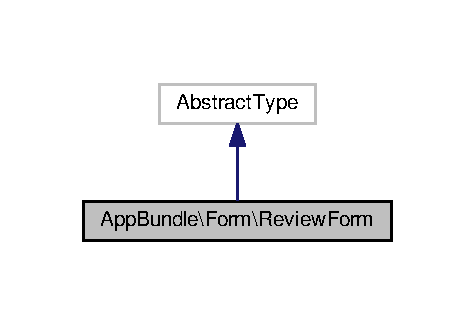
\includegraphics[width=228pt]{classAppBundle_1_1Form_1_1ReviewForm__inherit__graph}
\end{center}
\end{figure}


Graphe de collaboration de App\+Bundle\textbackslash{}Form\textbackslash{}Review\+Form\+:\nopagebreak
\begin{figure}[H]
\begin{center}
\leavevmode
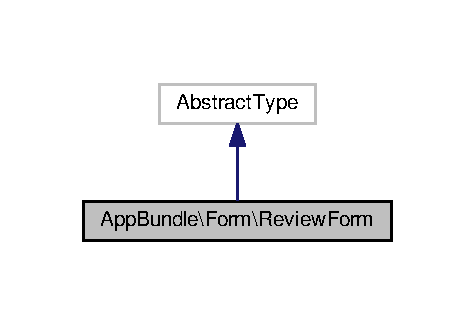
\includegraphics[width=228pt]{classAppBundle_1_1Form_1_1ReviewForm__coll__graph}
\end{center}
\end{figure}
\subsection*{Fonctions membres publiques}
\begin{DoxyCompactItemize}
\item 
\mbox{\Hypertarget{classAppBundle_1_1Form_1_1ReviewForm_a60e8dbe014408ee6d865b52e4b4db4e3}\label{classAppBundle_1_1Form_1_1ReviewForm_a60e8dbe014408ee6d865b52e4b4db4e3}} 
{\bfseries build\+Form} (Form\+Builder\+Interface \$builder, array \$options)
\item 
\mbox{\Hypertarget{classAppBundle_1_1Form_1_1ReviewForm_ab654af85b04d25657af117f69435fa59}\label{classAppBundle_1_1Form_1_1ReviewForm_ab654af85b04d25657af117f69435fa59}} 
{\bfseries configure\+Options} (Options\+Resolver \$resolver)
\end{DoxyCompactItemize}


La documentation de cette classe a été générée à partir du fichier suivant \+:\begin{DoxyCompactItemize}
\item 
src/\+App\+Bundle/\+Form/Review\+Form.\+php\end{DoxyCompactItemize}

\hypertarget{classAppBundle_1_1Repository_1_1ReviewRepository}{}\section{Référence de la classe App\+Bundle\textbackslash{}Repository\textbackslash{}Review\+Repository}
\label{classAppBundle_1_1Repository_1_1ReviewRepository}\index{App\+Bundle\textbackslash{}\+Repository\textbackslash{}\+Review\+Repository@{App\+Bundle\textbackslash{}\+Repository\textbackslash{}\+Review\+Repository}}


Graphe d\textquotesingle{}héritage de App\+Bundle\textbackslash{}Repository\textbackslash{}Review\+Repository\+:\nopagebreak
\begin{figure}[H]
\begin{center}
\leavevmode
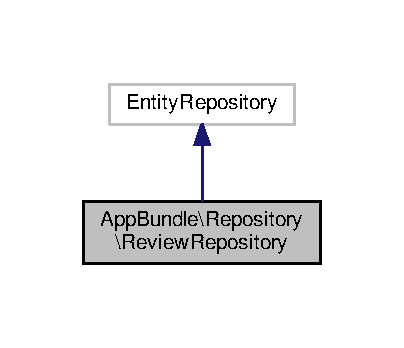
\includegraphics[width=194pt]{classAppBundle_1_1Repository_1_1ReviewRepository__inherit__graph}
\end{center}
\end{figure}


Graphe de collaboration de App\+Bundle\textbackslash{}Repository\textbackslash{}Review\+Repository\+:\nopagebreak
\begin{figure}[H]
\begin{center}
\leavevmode
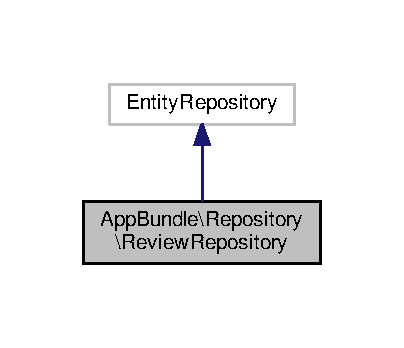
\includegraphics[width=194pt]{classAppBundle_1_1Repository_1_1ReviewRepository__coll__graph}
\end{center}
\end{figure}


\subsection{Description détaillée}
\hyperlink{classAppBundle_1_1Repository_1_1ReviewRepository}{Review\+Repository}

This class was generated by the \hyperlink{namespaceAppBundle_1_1Doctrine}{Doctrine} O\+RM. Add your own custom repository methods below. 

La documentation de cette classe a été générée à partir du fichier suivant \+:\begin{DoxyCompactItemize}
\item 
src/\+App\+Bundle/\+Repository/Review\+Repository.\+php\end{DoxyCompactItemize}

\hypertarget{classAppBundle_1_1Entity_1_1Role}{}\section{Référence de la classe App\+Bundle\textbackslash{}Entity\textbackslash{}Role}
\label{classAppBundle_1_1Entity_1_1Role}\index{App\+Bundle\textbackslash{}\+Entity\textbackslash{}\+Role@{App\+Bundle\textbackslash{}\+Entity\textbackslash{}\+Role}}
\subsection*{Fonctions membres publiques}
\begin{DoxyCompactItemize}
\item 
\hyperlink{classAppBundle_1_1Entity_1_1Role_ab30a055916446a86d21cbc622e29b91e}{get\+Id} ()
\item 
\hyperlink{classAppBundle_1_1Entity_1_1Role_a89328bdf2bb14c5c3f75bdafc2c26349}{set\+Role\+Name} (\$role\+Name)
\item 
\hyperlink{classAppBundle_1_1Entity_1_1Role_a421af5d35ceb62acd31c63645a092022}{get\+Role\+Name} ()
\item 
\hyperlink{classAppBundle_1_1Entity_1_1Role_a45fa2f158f13af1b3ccc5673075b814e}{set\+Is\+Admin} (\$\hyperlink{classAppBundle_1_1Entity_1_1Role_a288a7e5a21441f16a3ff077b37b27602}{is\+Admin})
\item 
\hyperlink{classAppBundle_1_1Entity_1_1Role_a288a7e5a21441f16a3ff077b37b27602}{is\+Admin} ()
\item 
\hyperlink{classAppBundle_1_1Entity_1_1Role_a82ea08d642dbfd8b35c0053e44b43ad3}{set\+Is\+Moderator} (\$\hyperlink{classAppBundle_1_1Entity_1_1Role_a659892168df4ecc1e6f447c297045240}{is\+Moderator})
\item 
\hyperlink{classAppBundle_1_1Entity_1_1Role_a659892168df4ecc1e6f447c297045240}{is\+Moderator} ()
\item 
\hyperlink{classAppBundle_1_1Entity_1_1Role_a9384e7e7881d3aac98361beb52dbbf6b}{set\+Role\+Color} (\$role\+Color)
\item 
\hyperlink{classAppBundle_1_1Entity_1_1Role_a09a2aeb58c083be3986f9dd823b7a1af}{get\+Role\+Color} ()
\item 
\hyperlink{classAppBundle_1_1Entity_1_1Role_a1c6633761909eb4de1c9bf91c4b739ff}{get\+Is\+Admin} ()
\item 
\hyperlink{classAppBundle_1_1Entity_1_1Role_a75e0500956054de38ff8729244986b4a}{get\+Is\+Moderator} ()
\end{DoxyCompactItemize}


\subsection{Description détaillée}
\hyperlink{classAppBundle_1_1Entity_1_1Role}{Role}

(name=\char`\"{}role\char`\"{}) (repository\+Class=\char`\"{}\+App\+Bundle\textbackslash{}\+Repository\textbackslash{}\+Role\+Repository\char`\"{}) 

\subsection{Documentation des fonctions membres}
\mbox{\Hypertarget{classAppBundle_1_1Entity_1_1Role_ab30a055916446a86d21cbc622e29b91e}\label{classAppBundle_1_1Entity_1_1Role_ab30a055916446a86d21cbc622e29b91e}} 
\index{App\+Bundle\+::\+Entity\+::\+Role@{App\+Bundle\+::\+Entity\+::\+Role}!get\+Id@{get\+Id}}
\index{get\+Id@{get\+Id}!App\+Bundle\+::\+Entity\+::\+Role@{App\+Bundle\+::\+Entity\+::\+Role}}
\subsubsection{\texorpdfstring{get\+Id()}{getId()}}
{\footnotesize\ttfamily App\+Bundle\textbackslash{}\+Entity\textbackslash{}\+Role\+::get\+Id (\begin{DoxyParamCaption}{ }\end{DoxyParamCaption})}

Get id

\begin{DoxyReturn}{Renvoie}
int 
\end{DoxyReturn}
\mbox{\Hypertarget{classAppBundle_1_1Entity_1_1Role_a1c6633761909eb4de1c9bf91c4b739ff}\label{classAppBundle_1_1Entity_1_1Role_a1c6633761909eb4de1c9bf91c4b739ff}} 
\index{App\+Bundle\+::\+Entity\+::\+Role@{App\+Bundle\+::\+Entity\+::\+Role}!get\+Is\+Admin@{get\+Is\+Admin}}
\index{get\+Is\+Admin@{get\+Is\+Admin}!App\+Bundle\+::\+Entity\+::\+Role@{App\+Bundle\+::\+Entity\+::\+Role}}
\subsubsection{\texorpdfstring{get\+Is\+Admin()}{getIsAdmin()}}
{\footnotesize\ttfamily App\+Bundle\textbackslash{}\+Entity\textbackslash{}\+Role\+::get\+Is\+Admin (\begin{DoxyParamCaption}{ }\end{DoxyParamCaption})}

Get is\+Admin

\begin{DoxyReturn}{Renvoie}
boolean 
\end{DoxyReturn}
\mbox{\Hypertarget{classAppBundle_1_1Entity_1_1Role_a75e0500956054de38ff8729244986b4a}\label{classAppBundle_1_1Entity_1_1Role_a75e0500956054de38ff8729244986b4a}} 
\index{App\+Bundle\+::\+Entity\+::\+Role@{App\+Bundle\+::\+Entity\+::\+Role}!get\+Is\+Moderator@{get\+Is\+Moderator}}
\index{get\+Is\+Moderator@{get\+Is\+Moderator}!App\+Bundle\+::\+Entity\+::\+Role@{App\+Bundle\+::\+Entity\+::\+Role}}
\subsubsection{\texorpdfstring{get\+Is\+Moderator()}{getIsModerator()}}
{\footnotesize\ttfamily App\+Bundle\textbackslash{}\+Entity\textbackslash{}\+Role\+::get\+Is\+Moderator (\begin{DoxyParamCaption}{ }\end{DoxyParamCaption})}

Get is\+Moderator

\begin{DoxyReturn}{Renvoie}
boolean 
\end{DoxyReturn}
\mbox{\Hypertarget{classAppBundle_1_1Entity_1_1Role_a09a2aeb58c083be3986f9dd823b7a1af}\label{classAppBundle_1_1Entity_1_1Role_a09a2aeb58c083be3986f9dd823b7a1af}} 
\index{App\+Bundle\+::\+Entity\+::\+Role@{App\+Bundle\+::\+Entity\+::\+Role}!get\+Role\+Color@{get\+Role\+Color}}
\index{get\+Role\+Color@{get\+Role\+Color}!App\+Bundle\+::\+Entity\+::\+Role@{App\+Bundle\+::\+Entity\+::\+Role}}
\subsubsection{\texorpdfstring{get\+Role\+Color()}{getRoleColor()}}
{\footnotesize\ttfamily App\+Bundle\textbackslash{}\+Entity\textbackslash{}\+Role\+::get\+Role\+Color (\begin{DoxyParamCaption}{ }\end{DoxyParamCaption})}

Get role\+Color

\begin{DoxyReturn}{Renvoie}
string 
\end{DoxyReturn}
\mbox{\Hypertarget{classAppBundle_1_1Entity_1_1Role_a421af5d35ceb62acd31c63645a092022}\label{classAppBundle_1_1Entity_1_1Role_a421af5d35ceb62acd31c63645a092022}} 
\index{App\+Bundle\+::\+Entity\+::\+Role@{App\+Bundle\+::\+Entity\+::\+Role}!get\+Role\+Name@{get\+Role\+Name}}
\index{get\+Role\+Name@{get\+Role\+Name}!App\+Bundle\+::\+Entity\+::\+Role@{App\+Bundle\+::\+Entity\+::\+Role}}
\subsubsection{\texorpdfstring{get\+Role\+Name()}{getRoleName()}}
{\footnotesize\ttfamily App\+Bundle\textbackslash{}\+Entity\textbackslash{}\+Role\+::get\+Role\+Name (\begin{DoxyParamCaption}{ }\end{DoxyParamCaption})}

Get role\+Name

\begin{DoxyReturn}{Renvoie}
string 
\end{DoxyReturn}
\mbox{\Hypertarget{classAppBundle_1_1Entity_1_1Role_a288a7e5a21441f16a3ff077b37b27602}\label{classAppBundle_1_1Entity_1_1Role_a288a7e5a21441f16a3ff077b37b27602}} 
\index{App\+Bundle\+::\+Entity\+::\+Role@{App\+Bundle\+::\+Entity\+::\+Role}!is\+Admin@{is\+Admin}}
\index{is\+Admin@{is\+Admin}!App\+Bundle\+::\+Entity\+::\+Role@{App\+Bundle\+::\+Entity\+::\+Role}}
\subsubsection{\texorpdfstring{is\+Admin()}{isAdmin()}}
{\footnotesize\ttfamily App\+Bundle\textbackslash{}\+Entity\textbackslash{}\+Role\+::is\+Admin (\begin{DoxyParamCaption}{ }\end{DoxyParamCaption})}

Get is\+Admin

\begin{DoxyReturn}{Renvoie}
boolean 
\end{DoxyReturn}
\mbox{\Hypertarget{classAppBundle_1_1Entity_1_1Role_a659892168df4ecc1e6f447c297045240}\label{classAppBundle_1_1Entity_1_1Role_a659892168df4ecc1e6f447c297045240}} 
\index{App\+Bundle\+::\+Entity\+::\+Role@{App\+Bundle\+::\+Entity\+::\+Role}!is\+Moderator@{is\+Moderator}}
\index{is\+Moderator@{is\+Moderator}!App\+Bundle\+::\+Entity\+::\+Role@{App\+Bundle\+::\+Entity\+::\+Role}}
\subsubsection{\texorpdfstring{is\+Moderator()}{isModerator()}}
{\footnotesize\ttfamily App\+Bundle\textbackslash{}\+Entity\textbackslash{}\+Role\+::is\+Moderator (\begin{DoxyParamCaption}{ }\end{DoxyParamCaption})}

Get is\+Moderator

\begin{DoxyReturn}{Renvoie}
boolean 
\end{DoxyReturn}
\mbox{\Hypertarget{classAppBundle_1_1Entity_1_1Role_a45fa2f158f13af1b3ccc5673075b814e}\label{classAppBundle_1_1Entity_1_1Role_a45fa2f158f13af1b3ccc5673075b814e}} 
\index{App\+Bundle\+::\+Entity\+::\+Role@{App\+Bundle\+::\+Entity\+::\+Role}!set\+Is\+Admin@{set\+Is\+Admin}}
\index{set\+Is\+Admin@{set\+Is\+Admin}!App\+Bundle\+::\+Entity\+::\+Role@{App\+Bundle\+::\+Entity\+::\+Role}}
\subsubsection{\texorpdfstring{set\+Is\+Admin()}{setIsAdmin()}}
{\footnotesize\ttfamily App\+Bundle\textbackslash{}\+Entity\textbackslash{}\+Role\+::set\+Is\+Admin (\begin{DoxyParamCaption}\item[{}]{\$is\+Admin }\end{DoxyParamCaption})}

Set is\+Admin


\begin{DoxyParams}[1]{Paramètres}
boolean & {\em \$is\+Admin} & \\
\hline
\end{DoxyParams}
\begin{DoxyReturn}{Renvoie}
\hyperlink{classAppBundle_1_1Entity_1_1Role}{Role} 
\end{DoxyReturn}
\mbox{\Hypertarget{classAppBundle_1_1Entity_1_1Role_a82ea08d642dbfd8b35c0053e44b43ad3}\label{classAppBundle_1_1Entity_1_1Role_a82ea08d642dbfd8b35c0053e44b43ad3}} 
\index{App\+Bundle\+::\+Entity\+::\+Role@{App\+Bundle\+::\+Entity\+::\+Role}!set\+Is\+Moderator@{set\+Is\+Moderator}}
\index{set\+Is\+Moderator@{set\+Is\+Moderator}!App\+Bundle\+::\+Entity\+::\+Role@{App\+Bundle\+::\+Entity\+::\+Role}}
\subsubsection{\texorpdfstring{set\+Is\+Moderator()}{setIsModerator()}}
{\footnotesize\ttfamily App\+Bundle\textbackslash{}\+Entity\textbackslash{}\+Role\+::set\+Is\+Moderator (\begin{DoxyParamCaption}\item[{}]{\$is\+Moderator }\end{DoxyParamCaption})}

Set is\+Moderator


\begin{DoxyParams}[1]{Paramètres}
boolean & {\em \$is\+Moderator} & \\
\hline
\end{DoxyParams}
\begin{DoxyReturn}{Renvoie}
\hyperlink{classAppBundle_1_1Entity_1_1Role}{Role} 
\end{DoxyReturn}
\mbox{\Hypertarget{classAppBundle_1_1Entity_1_1Role_a9384e7e7881d3aac98361beb52dbbf6b}\label{classAppBundle_1_1Entity_1_1Role_a9384e7e7881d3aac98361beb52dbbf6b}} 
\index{App\+Bundle\+::\+Entity\+::\+Role@{App\+Bundle\+::\+Entity\+::\+Role}!set\+Role\+Color@{set\+Role\+Color}}
\index{set\+Role\+Color@{set\+Role\+Color}!App\+Bundle\+::\+Entity\+::\+Role@{App\+Bundle\+::\+Entity\+::\+Role}}
\subsubsection{\texorpdfstring{set\+Role\+Color()}{setRoleColor()}}
{\footnotesize\ttfamily App\+Bundle\textbackslash{}\+Entity\textbackslash{}\+Role\+::set\+Role\+Color (\begin{DoxyParamCaption}\item[{}]{\$role\+Color }\end{DoxyParamCaption})}

Set role\+Color


\begin{DoxyParams}[1]{Paramètres}
string & {\em \$role\+Color} & \\
\hline
\end{DoxyParams}
\begin{DoxyReturn}{Renvoie}
\hyperlink{classAppBundle_1_1Entity_1_1Role}{Role} 
\end{DoxyReturn}
\mbox{\Hypertarget{classAppBundle_1_1Entity_1_1Role_a89328bdf2bb14c5c3f75bdafc2c26349}\label{classAppBundle_1_1Entity_1_1Role_a89328bdf2bb14c5c3f75bdafc2c26349}} 
\index{App\+Bundle\+::\+Entity\+::\+Role@{App\+Bundle\+::\+Entity\+::\+Role}!set\+Role\+Name@{set\+Role\+Name}}
\index{set\+Role\+Name@{set\+Role\+Name}!App\+Bundle\+::\+Entity\+::\+Role@{App\+Bundle\+::\+Entity\+::\+Role}}
\subsubsection{\texorpdfstring{set\+Role\+Name()}{setRoleName()}}
{\footnotesize\ttfamily App\+Bundle\textbackslash{}\+Entity\textbackslash{}\+Role\+::set\+Role\+Name (\begin{DoxyParamCaption}\item[{}]{\$role\+Name }\end{DoxyParamCaption})}

Set role\+Name


\begin{DoxyParams}[1]{Paramètres}
string & {\em \$role\+Name} & \\
\hline
\end{DoxyParams}
\begin{DoxyReturn}{Renvoie}
\hyperlink{classAppBundle_1_1Entity_1_1Role}{Role} 
\end{DoxyReturn}


La documentation de cette classe a été générée à partir du fichier suivant \+:\begin{DoxyCompactItemize}
\item 
src/\+App\+Bundle/\+Entity/Role.\+php\end{DoxyCompactItemize}

\hypertarget{classAppBundle_1_1Repository_1_1RoleRepository}{}\section{Référence de la classe App\+Bundle\textbackslash{}Repository\textbackslash{}Role\+Repository}
\label{classAppBundle_1_1Repository_1_1RoleRepository}\index{App\+Bundle\textbackslash{}\+Repository\textbackslash{}\+Role\+Repository@{App\+Bundle\textbackslash{}\+Repository\textbackslash{}\+Role\+Repository}}


Graphe d\textquotesingle{}héritage de App\+Bundle\textbackslash{}Repository\textbackslash{}Role\+Repository\+:\nopagebreak
\begin{figure}[H]
\begin{center}
\leavevmode
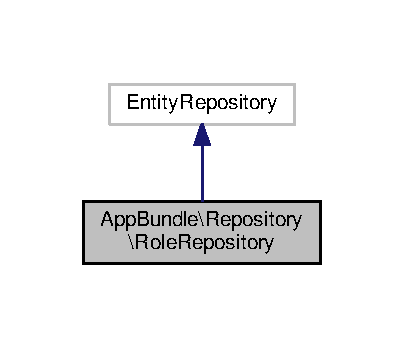
\includegraphics[width=194pt]{classAppBundle_1_1Repository_1_1RoleRepository__inherit__graph}
\end{center}
\end{figure}


Graphe de collaboration de App\+Bundle\textbackslash{}Repository\textbackslash{}Role\+Repository\+:\nopagebreak
\begin{figure}[H]
\begin{center}
\leavevmode
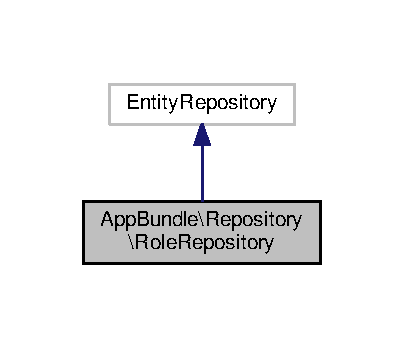
\includegraphics[width=194pt]{classAppBundle_1_1Repository_1_1RoleRepository__coll__graph}
\end{center}
\end{figure}


\subsection{Description détaillée}
\hyperlink{classAppBundle_1_1Repository_1_1RoleRepository}{Role\+Repository}

This class was generated by the \hyperlink{namespaceAppBundle_1_1Doctrine}{Doctrine} O\+RM. Add your own custom repository methods below. 

La documentation de cette classe a été générée à partir du fichier suivant \+:\begin{DoxyCompactItemize}
\item 
src/\+App\+Bundle/\+Repository/Role\+Repository.\+php\end{DoxyCompactItemize}

\hypertarget{classAppBundle_1_1Controller_1_1SecurityController}{}\section{Référence de la classe App\+Bundle\textbackslash{}Controller\textbackslash{}Security\+Controller}
\label{classAppBundle_1_1Controller_1_1SecurityController}\index{App\+Bundle\textbackslash{}\+Controller\textbackslash{}\+Security\+Controller@{App\+Bundle\textbackslash{}\+Controller\textbackslash{}\+Security\+Controller}}


Graphe d\textquotesingle{}héritage de App\+Bundle\textbackslash{}Controller\textbackslash{}Security\+Controller\+:\nopagebreak
\begin{figure}[H]
\begin{center}
\leavevmode
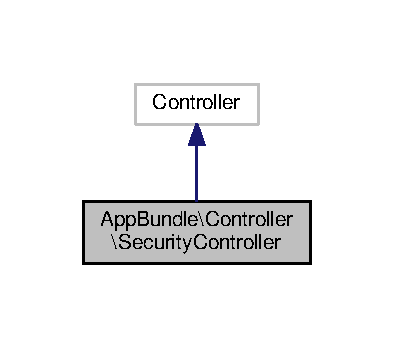
\includegraphics[width=189pt]{classAppBundle_1_1Controller_1_1SecurityController__inherit__graph}
\end{center}
\end{figure}


Graphe de collaboration de App\+Bundle\textbackslash{}Controller\textbackslash{}Security\+Controller\+:\nopagebreak
\begin{figure}[H]
\begin{center}
\leavevmode
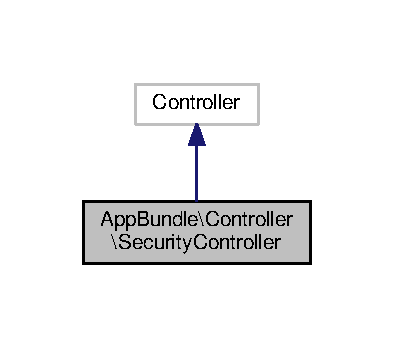
\includegraphics[width=189pt]{classAppBundle_1_1Controller_1_1SecurityController__coll__graph}
\end{center}
\end{figure}
\subsection*{Fonctions membres publiques}
\begin{DoxyCompactItemize}
\item 
\hyperlink{classAppBundle_1_1Controller_1_1SecurityController_ac211800b0754333fd74c47600d369aad}{register\+Action} (Request \$request)
\item 
\hyperlink{classAppBundle_1_1Controller_1_1SecurityController_a6a941512644667b9eed55538fc8934a8}{login\+Action} (Request \$request)
\item 
\hyperlink{classAppBundle_1_1Controller_1_1SecurityController_a8624fe4c796f910e349c874ff5d73ad2}{logout\+Action} ()
\end{DoxyCompactItemize}


\subsection{Documentation des fonctions membres}
\mbox{\Hypertarget{classAppBundle_1_1Controller_1_1SecurityController_a6a941512644667b9eed55538fc8934a8}\label{classAppBundle_1_1Controller_1_1SecurityController_a6a941512644667b9eed55538fc8934a8}} 
\index{App\+Bundle\+::\+Controller\+::\+Security\+Controller@{App\+Bundle\+::\+Controller\+::\+Security\+Controller}!login\+Action@{login\+Action}}
\index{login\+Action@{login\+Action}!App\+Bundle\+::\+Controller\+::\+Security\+Controller@{App\+Bundle\+::\+Controller\+::\+Security\+Controller}}
\subsubsection{\texorpdfstring{login\+Action()}{loginAction()}}
{\footnotesize\ttfamily App\+Bundle\textbackslash{}\+Controller\textbackslash{}\+Security\+Controller\+::login\+Action (\begin{DoxyParamCaption}\item[{Request}]{\$request }\end{DoxyParamCaption})}

(\char`\"{}/login\char`\"{}, name=\char`\"{}login\char`\"{}) 
\begin{DoxyParams}[1]{Paramètres}
Request & {\em \$request} & \\
\hline
\end{DoxyParams}
\begin{DoxyReturn}{Renvoie}
Redirect\+Response$\vert$\+Response 
\end{DoxyReturn}
\mbox{\Hypertarget{classAppBundle_1_1Controller_1_1SecurityController_a8624fe4c796f910e349c874ff5d73ad2}\label{classAppBundle_1_1Controller_1_1SecurityController_a8624fe4c796f910e349c874ff5d73ad2}} 
\index{App\+Bundle\+::\+Controller\+::\+Security\+Controller@{App\+Bundle\+::\+Controller\+::\+Security\+Controller}!logout\+Action@{logout\+Action}}
\index{logout\+Action@{logout\+Action}!App\+Bundle\+::\+Controller\+::\+Security\+Controller@{App\+Bundle\+::\+Controller\+::\+Security\+Controller}}
\subsubsection{\texorpdfstring{logout\+Action()}{logoutAction()}}
{\footnotesize\ttfamily App\+Bundle\textbackslash{}\+Controller\textbackslash{}\+Security\+Controller\+::logout\+Action (\begin{DoxyParamCaption}{ }\end{DoxyParamCaption})}

Route de déconexion

(\char`\"{}/logout\char`\"{}, name=\char`\"{}logout\char`\"{}) \mbox{\Hypertarget{classAppBundle_1_1Controller_1_1SecurityController_ac211800b0754333fd74c47600d369aad}\label{classAppBundle_1_1Controller_1_1SecurityController_ac211800b0754333fd74c47600d369aad}} 
\index{App\+Bundle\+::\+Controller\+::\+Security\+Controller@{App\+Bundle\+::\+Controller\+::\+Security\+Controller}!register\+Action@{register\+Action}}
\index{register\+Action@{register\+Action}!App\+Bundle\+::\+Controller\+::\+Security\+Controller@{App\+Bundle\+::\+Controller\+::\+Security\+Controller}}
\subsubsection{\texorpdfstring{register\+Action()}{registerAction()}}
{\footnotesize\ttfamily App\+Bundle\textbackslash{}\+Controller\textbackslash{}\+Security\+Controller\+::register\+Action (\begin{DoxyParamCaption}\item[{Request}]{\$request }\end{DoxyParamCaption})}

(\char`\"{}/register\char`\"{}, name=\char`\"{}register\char`\"{}) 
\begin{DoxyParams}[1]{Paramètres}
Request & {\em \$request} & \\
\hline
\end{DoxyParams}
\begin{DoxyReturn}{Renvoie}
Response 
\end{DoxyReturn}


La documentation de cette classe a été générée à partir du fichier suivant \+:\begin{DoxyCompactItemize}
\item 
src/\+App\+Bundle/\+Controller/Security\+Controller.\+php\end{DoxyCompactItemize}

\hypertarget{classTests_1_1AppBundle_1_1Controller_1_1SecurityControllerTest}{}\section{Référence de la classe Tests\textbackslash{}App\+Bundle\textbackslash{}Controller\textbackslash{}Security\+Controller\+Test}
\label{classTests_1_1AppBundle_1_1Controller_1_1SecurityControllerTest}\index{Tests\textbackslash{}\+App\+Bundle\textbackslash{}\+Controller\textbackslash{}\+Security\+Controller\+Test@{Tests\textbackslash{}\+App\+Bundle\textbackslash{}\+Controller\textbackslash{}\+Security\+Controller\+Test}}


Graphe d\textquotesingle{}héritage de Tests\textbackslash{}App\+Bundle\textbackslash{}Controller\textbackslash{}Security\+Controller\+Test\+:\nopagebreak
\begin{figure}[H]
\begin{center}
\leavevmode
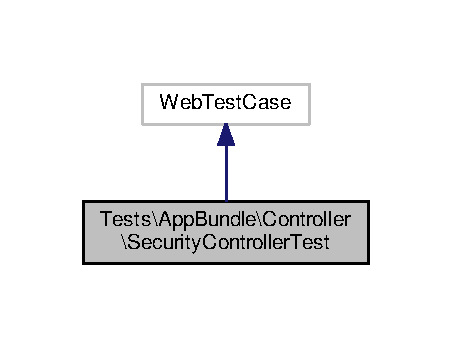
\includegraphics[width=217pt]{classTests_1_1AppBundle_1_1Controller_1_1SecurityControllerTest__inherit__graph}
\end{center}
\end{figure}


Graphe de collaboration de Tests\textbackslash{}App\+Bundle\textbackslash{}Controller\textbackslash{}Security\+Controller\+Test\+:\nopagebreak
\begin{figure}[H]
\begin{center}
\leavevmode
\includegraphics[width=217pt]{classTests_1_1AppBundle_1_1Controller_1_1SecurityControllerTest__coll__graph}
\end{center}
\end{figure}
\subsection*{Fonctions membres publiques}
\begin{DoxyCompactItemize}
\item 
\mbox{\Hypertarget{classTests_1_1AppBundle_1_1Controller_1_1SecurityControllerTest_a872bb08c3d26d51796c757c8e2df5a81}\label{classTests_1_1AppBundle_1_1Controller_1_1SecurityControllerTest_a872bb08c3d26d51796c757c8e2df5a81}} 
{\bfseries test\+Register} ()
\end{DoxyCompactItemize}


La documentation de cette classe a été générée à partir du fichier suivant \+:\begin{DoxyCompactItemize}
\item 
tests/\+App\+Bundle/\+Controller/Security\+Controller\+Test.\+php\end{DoxyCompactItemize}

\hypertarget{classSymfonyRequirements}{}\section{Référence de la classe Symfony\+Requirements}
\label{classSymfonyRequirements}\index{Symfony\+Requirements@{Symfony\+Requirements}}


Graphe d\textquotesingle{}héritage de Symfony\+Requirements\+:\nopagebreak
\begin{figure}[H]
\begin{center}
\leavevmode
\includegraphics[width=196pt]{classSymfonyRequirements__inherit__graph}
\end{center}
\end{figure}


Graphe de collaboration de Symfony\+Requirements\+:\nopagebreak
\begin{figure}[H]
\begin{center}
\leavevmode
\includegraphics[width=196pt]{classSymfonyRequirements__coll__graph}
\end{center}
\end{figure}
\subsection*{Fonctions membres publiques}
\begin{DoxyCompactItemize}
\item 
\hyperlink{classSymfonyRequirements_a9543e8a8cb4c134200fd19a3052cac38}{\+\_\+\+\_\+construct} ()
\end{DoxyCompactItemize}
\subsection*{Attributs publics}
\begin{DoxyCompactItemize}
\item 
\mbox{\Hypertarget{classSymfonyRequirements_aadd8789c5e6de1ef1b13c78dcf985a28}\label{classSymfonyRequirements_aadd8789c5e6de1ef1b13c78dcf985a28}} 
const {\bfseries L\+E\+G\+A\+C\+Y\+\_\+\+R\+E\+Q\+U\+I\+R\+E\+D\+\_\+\+P\+H\+P\+\_\+\+V\+E\+R\+S\+I\+ON} = \textquotesingle{}5.\+3.\+3\textquotesingle{}
\item 
\mbox{\Hypertarget{classSymfonyRequirements_af0e0b5455bf96b10af63695ab61c5137}\label{classSymfonyRequirements_af0e0b5455bf96b10af63695ab61c5137}} 
const {\bfseries R\+E\+Q\+U\+I\+R\+E\+D\+\_\+\+P\+H\+P\+\_\+\+V\+E\+R\+S\+I\+ON} = \textquotesingle{}5.\+5.\+9\textquotesingle{}
\end{DoxyCompactItemize}
\subsection*{Fonctions membres protégées}
\begin{DoxyCompactItemize}
\item 
\hyperlink{classSymfonyRequirements_a32cc5be91d7f8049b0f49ef118e2cd04}{get\+Realpath\+Cache\+Size} ()
\item 
\hyperlink{classSymfonyRequirements_ae0578284b71aadf39c3457fc5d3f5aa1}{get\+Php\+Required\+Version} ()
\end{DoxyCompactItemize}


\subsection{Description détaillée}
This class specifies all requirements and optional recommendations that are necessary to run the Symfony Standard Edition.

\begin{DoxyAuthor}{Auteur}
Tobias Schultze \href{http://tobion.de}{\tt http\+://tobion.\+de} 

Fabien Potencier \href{mailto:fabien@symfony.com}{\tt fabien@symfony.\+com} 
\end{DoxyAuthor}


\subsection{Documentation des constructeurs et destructeur}
\mbox{\Hypertarget{classSymfonyRequirements_a9543e8a8cb4c134200fd19a3052cac38}\label{classSymfonyRequirements_a9543e8a8cb4c134200fd19a3052cac38}} 
\index{Symfony\+Requirements@{Symfony\+Requirements}!\+\_\+\+\_\+construct@{\+\_\+\+\_\+construct}}
\index{\+\_\+\+\_\+construct@{\+\_\+\+\_\+construct}!Symfony\+Requirements@{Symfony\+Requirements}}
\subsubsection{\texorpdfstring{\+\_\+\+\_\+construct()}{\_\_construct()}}
{\footnotesize\ttfamily Symfony\+Requirements\+::\+\_\+\+\_\+construct (\begin{DoxyParamCaption}{ }\end{DoxyParamCaption})}

Constructor that initializes the requirements. 

\subsection{Documentation des fonctions membres}
\mbox{\Hypertarget{classSymfonyRequirements_ae0578284b71aadf39c3457fc5d3f5aa1}\label{classSymfonyRequirements_ae0578284b71aadf39c3457fc5d3f5aa1}} 
\index{Symfony\+Requirements@{Symfony\+Requirements}!get\+Php\+Required\+Version@{get\+Php\+Required\+Version}}
\index{get\+Php\+Required\+Version@{get\+Php\+Required\+Version}!Symfony\+Requirements@{Symfony\+Requirements}}
\subsubsection{\texorpdfstring{get\+Php\+Required\+Version()}{getPhpRequiredVersion()}}
{\footnotesize\ttfamily Symfony\+Requirements\+::get\+Php\+Required\+Version (\begin{DoxyParamCaption}{ }\end{DoxyParamCaption})\hspace{0.3cm}{\ttfamily [protected]}}

Defines P\+HP required version from Symfony version.

\begin{DoxyReturn}{Renvoie}
string$\vert$false The P\+HP required version or false if it could not be guessed 
\end{DoxyReturn}
\mbox{\Hypertarget{classSymfonyRequirements_a32cc5be91d7f8049b0f49ef118e2cd04}\label{classSymfonyRequirements_a32cc5be91d7f8049b0f49ef118e2cd04}} 
\index{Symfony\+Requirements@{Symfony\+Requirements}!get\+Realpath\+Cache\+Size@{get\+Realpath\+Cache\+Size}}
\index{get\+Realpath\+Cache\+Size@{get\+Realpath\+Cache\+Size}!Symfony\+Requirements@{Symfony\+Requirements}}
\subsubsection{\texorpdfstring{get\+Realpath\+Cache\+Size()}{getRealpathCacheSize()}}
{\footnotesize\ttfamily Symfony\+Requirements\+::get\+Realpath\+Cache\+Size (\begin{DoxyParamCaption}{ }\end{DoxyParamCaption})\hspace{0.3cm}{\ttfamily [protected]}}

Loads realpath\+\_\+cache\+\_\+size from php.\+ini and converts it to int.

(e.\+g. 16k is converted to 16384 int)

\begin{DoxyReturn}{Renvoie}
int 
\end{DoxyReturn}


La documentation de cette classe a été générée à partir du fichier suivant \+:\begin{DoxyCompactItemize}
\item 
var/Symfony\+Requirements.\+php\end{DoxyCompactItemize}

\hypertarget{classAppBundle_1_1Entity_1_1User}{}\section{Référence de la classe App\+Bundle\textbackslash{}Entity\textbackslash{}User}
\label{classAppBundle_1_1Entity_1_1User}\index{App\+Bundle\textbackslash{}\+Entity\textbackslash{}\+User@{App\+Bundle\textbackslash{}\+Entity\textbackslash{}\+User}}


Graphe d\textquotesingle{}héritage de App\+Bundle\textbackslash{}Entity\textbackslash{}User\+:\nopagebreak
\begin{figure}[H]
\begin{center}
\leavevmode
\includegraphics[width=350pt]{classAppBundle_1_1Entity_1_1User__inherit__graph}
\end{center}
\end{figure}


Graphe de collaboration de App\+Bundle\textbackslash{}Entity\textbackslash{}User\+:\nopagebreak
\begin{figure}[H]
\begin{center}
\leavevmode
\includegraphics[width=350pt]{classAppBundle_1_1Entity_1_1User__coll__graph}
\end{center}
\end{figure}
\subsection*{Fonctions membres publiques}
\begin{DoxyCompactItemize}
\item 
\hyperlink{classAppBundle_1_1Entity_1_1User_aaa021257dad62d5358521ff7b99face1}{get\+Id} ()
\item 
\hyperlink{classAppBundle_1_1Entity_1_1User_a9f6b20493060944536b750b40b4471e3}{set\+Username} (\$username)
\item 
\hyperlink{classAppBundle_1_1Entity_1_1User_abfb46cc3484bde6475517e11fc39688e}{get\+Username} ()
\item 
\hyperlink{classAppBundle_1_1Entity_1_1User_aee5056e27aa8e27ca38af6e6373f99e8}{set\+Password} (\$password)
\item 
\hyperlink{classAppBundle_1_1Entity_1_1User_ad3e3f65ed144a768cad99df4d588cd63}{get\+Password} ()
\item 
\hyperlink{classAppBundle_1_1Entity_1_1User_a717949a66aa01fdba29d464294d60723}{set\+Email} (\$email)
\item 
\hyperlink{classAppBundle_1_1Entity_1_1User_a20d5e560b025fd5248ad680749f7c79c}{get\+Email} ()
\item 
\hyperlink{classAppBundle_1_1Entity_1_1User_acf0e0a3188e796f7a9bc40a66b1cca12}{set\+Avatar} (\$avatar)
\item 
\hyperlink{classAppBundle_1_1Entity_1_1User_a770921ad3fbe7019a53d0dd7a3ec1328}{get\+Avatar} ()
\item 
\hyperlink{classAppBundle_1_1Entity_1_1User_af69d6db9253e066027e55c07c209b392}{set\+Description} (\$description)
\item 
\hyperlink{classAppBundle_1_1Entity_1_1User_abdbd6231b898b07d0a159bd0f254770c}{get\+Description} ()
\item 
\hyperlink{classAppBundle_1_1Entity_1_1User_a7feac9233be86c6fd93280a891905a2b}{get\+Roles} ()
\item 
\hyperlink{classAppBundle_1_1Entity_1_1User_a5c4b12b13068e7e0ff2fe3e773ef16ee}{get\+Salt} ()
\item 
\hyperlink{classAppBundle_1_1Entity_1_1User_adc1ae82385690849964ace63e84a1321}{erase\+Credentials} ()
\item 
\hyperlink{classAppBundle_1_1Entity_1_1User_a3e00ef768aa0cac041abfda0d164bfcb}{\+\_\+\+\_\+construct} ()
\item 
\hyperlink{classAppBundle_1_1Entity_1_1User_ad089e5a875b330dcc623176a025df18a}{add\+Friend} (\hyperlink{classAppBundle_1_1Entity_1_1User}{User} \$friend)
\item 
\hyperlink{classAppBundle_1_1Entity_1_1User_a2f11445931ce2da98849005f7818577b}{remove\+Friend} (\hyperlink{classAppBundle_1_1Entity_1_1User}{User} \$friend)
\item 
\hyperlink{classAppBundle_1_1Entity_1_1User_aedd7fe474663d7d06a917dd6862ab6db}{get\+Friends} ()
\item 
\mbox{\Hypertarget{classAppBundle_1_1Entity_1_1User_a233d60bd0f45895227c6e56942dbf559}\label{classAppBundle_1_1Entity_1_1User_a233d60bd0f45895227c6e56942dbf559}} 
{\bfseries add\+Friend\+Both\+Ways} (\hyperlink{classAppBundle_1_1Entity_1_1User}{User} \$user)
\item 
\mbox{\Hypertarget{classAppBundle_1_1Entity_1_1User_ad6d2942e951c6fbeb9b4e6d72eecc579}\label{classAppBundle_1_1Entity_1_1User_ad6d2942e951c6fbeb9b4e6d72eecc579}} 
{\bfseries remove\+Friend\+Both\+Ways} (\hyperlink{classAppBundle_1_1Entity_1_1User}{User} \$user)
\item 
\hyperlink{classAppBundle_1_1Entity_1_1User_abfd09d2156ac2c22b69a04690fd6977c}{set\+Plain\+Password} (\$plain\+Password)
\item 
\hyperlink{classAppBundle_1_1Entity_1_1User_a5cdc0aeccfeb1a06f9fa8d9032545ebf}{get\+Plain\+Password} ()
\item 
\hyperlink{classAppBundle_1_1Entity_1_1User_aea0ec322bcefd3f64da757770bb3a8a8}{serialize} ()
\item 
\hyperlink{classAppBundle_1_1Entity_1_1User_a35b5a8b6198e5c57b7cc176ba46c19d0}{unserialize} (\$serialized)
\item 
\hyperlink{classAppBundle_1_1Entity_1_1User_a6e8354db28000b0b61faace41a09ff7f}{is\+Equal\+To} (User\+Interface \$user)
\item 
\hyperlink{classAppBundle_1_1Entity_1_1User_a9a31aabdc1f483e3fab33c4c4d52b503}{set\+Private\+Key} (\$private\+Key)
\item 
\hyperlink{classAppBundle_1_1Entity_1_1User_a76dfaf3327def5913cee32e0bd91afaa}{get\+Private\+Key} ()
\item 
\hyperlink{classAppBundle_1_1Entity_1_1User_ac87d00e19c676f595d46bf4b0e203595}{set\+Date\+Inscription} (\$date\+Inscription)
\item 
\hyperlink{classAppBundle_1_1Entity_1_1User_ac33fea30003f3b00cdf87f0251bab415}{get\+Date\+Inscription} ()
\item 
\hyperlink{classAppBundle_1_1Entity_1_1User_ac8d0736d889ebc08338ad70f69765369}{add\+Pending\+Friend\+Request} (\textbackslash{}\hyperlink{classAppBundle_1_1Entity_1_1User}{App\+Bundle\textbackslash{}\+Entity\textbackslash{}\+User} \$pending\+Friend\+Request)
\item 
\hyperlink{classAppBundle_1_1Entity_1_1User_a551c41da5b479d91f9dadb9ae6de1ea7}{remove\+Pending\+Friend\+Request} (\textbackslash{}\hyperlink{classAppBundle_1_1Entity_1_1User}{App\+Bundle\textbackslash{}\+Entity\textbackslash{}\+User} \$pending\+Friend\+Request)
\item 
\hyperlink{classAppBundle_1_1Entity_1_1User_a8adb6142b8443d5cb2b63c55327f067b}{get\+Pending\+Friend\+Requests} ()
\item 
\hyperlink{classAppBundle_1_1Entity_1_1User_ab1eb464976d6d6b645100348a7eb59fd}{set\+Role} (\textbackslash{}\hyperlink{classAppBundle_1_1Entity_1_1Role}{App\+Bundle\textbackslash{}\+Entity\textbackslash{}\+Role} \$role)
\item 
\hyperlink{classAppBundle_1_1Entity_1_1User_a6481a9707a292bce8e9aebcf97f57721}{get\+Role} ()
\item 
\hyperlink{classAppBundle_1_1Entity_1_1User_a80ba0ef78ad298274abe11cbc6b7e5dc}{add\+Favorite} (\textbackslash{}\hyperlink{classAppBundle_1_1Entity_1_1Favorite}{App\+Bundle\textbackslash{}\+Entity\textbackslash{}\+Favorite} \$favorite)
\item 
\hyperlink{classAppBundle_1_1Entity_1_1User_af7cb4c6bea6a124059f98953dd77d21b}{remove\+Favorite} (\textbackslash{}\hyperlink{classAppBundle_1_1Entity_1_1Favorite}{App\+Bundle\textbackslash{}\+Entity\textbackslash{}\+Favorite} \$favorite)
\item 
\hyperlink{classAppBundle_1_1Entity_1_1User_aa3edb74a8f3d7af87a13530706583967}{get\+Favorites} ()
\item 
\hyperlink{classAppBundle_1_1Entity_1_1User_a3eb7c1f0d489635d719d2b31ffa13fb2}{set\+Markers} (\$markers)
\item 
\hyperlink{classAppBundle_1_1Entity_1_1User_acc8771e3c9635a1b8839f32a51c4fb34}{get\+Markers} ()
\item 
\hyperlink{classAppBundle_1_1Entity_1_1User_af69ae82da33c9232d1eca16653076ac3}{set\+Cities} (\$cities)
\item 
\hyperlink{classAppBundle_1_1Entity_1_1User_a81b6376d8ea4d57d8e60252f63582ea7}{get\+Cities} ()
\item 
\hyperlink{classAppBundle_1_1Entity_1_1User_ad59ebbe8eb918cc31422beeebbaa9b6c}{add\+Event} (\textbackslash{}\hyperlink{classAppBundle_1_1Entity_1_1Event}{App\+Bundle\textbackslash{}\+Entity\textbackslash{}\+Event} \$event)
\item 
\hyperlink{classAppBundle_1_1Entity_1_1User_a489a840a6fda94d0d811cd4c6294357f}{remove\+Event} (\textbackslash{}\hyperlink{classAppBundle_1_1Entity_1_1Event}{App\+Bundle\textbackslash{}\+Entity\textbackslash{}\+Event} \$event)
\item 
\hyperlink{classAppBundle_1_1Entity_1_1User_a62fde34b4402150a87ac4fd1e2cd5131}{get\+Events} ()
\item 
\hyperlink{classAppBundle_1_1Entity_1_1User_a4fa2fe6e700686a54540db892955f6dc}{add\+Review} (\textbackslash{}\hyperlink{classAppBundle_1_1Entity_1_1Review}{App\+Bundle\textbackslash{}\+Entity\textbackslash{}\+Review} \$review)
\item 
\hyperlink{classAppBundle_1_1Entity_1_1User_aed23331dfb185937f4ba5330bd70f9b5}{remove\+Review} (\textbackslash{}\hyperlink{classAppBundle_1_1Entity_1_1Review}{App\+Bundle\textbackslash{}\+Entity\textbackslash{}\+Review} \$review)
\item 
\hyperlink{classAppBundle_1_1Entity_1_1User_a29c6f462a5c30617e4f698a546ebd01c}{get\+Reviews} ()
\item 
\hyperlink{classAppBundle_1_1Entity_1_1User_a3368f692f4cbd77041ae379ea82d7d8e}{add\+Comment} (\textbackslash{}\hyperlink{classAppBundle_1_1Entity_1_1EventComment}{App\+Bundle\textbackslash{}\+Entity\textbackslash{}\+Event\+Comment} \$comment)
\item 
\hyperlink{classAppBundle_1_1Entity_1_1User_ad339056b59c0cb14cf5707ffd91a44a3}{remove\+Comment} (\textbackslash{}\hyperlink{classAppBundle_1_1Entity_1_1EventComment}{App\+Bundle\textbackslash{}\+Entity\textbackslash{}\+Event\+Comment} \$comment)
\item 
\hyperlink{classAppBundle_1_1Entity_1_1User_a8fbe81b221f53f304670755352cd470c}{get\+Comments} ()
\end{DoxyCompactItemize}


\subsection{Description détaillée}
\hyperlink{classAppBundle_1_1Entity_1_1User}{User}

(name=\char`\"{}user\char`\"{}) (repository\+Class=\char`\"{}\+App\+Bundle\textbackslash{}\+Repository\textbackslash{}\+User\+Repository\char`\"{}) 

\subsection{Documentation des constructeurs et destructeur}
\mbox{\Hypertarget{classAppBundle_1_1Entity_1_1User_a3e00ef768aa0cac041abfda0d164bfcb}\label{classAppBundle_1_1Entity_1_1User_a3e00ef768aa0cac041abfda0d164bfcb}} 
\index{App\+Bundle\+::\+Entity\+::\+User@{App\+Bundle\+::\+Entity\+::\+User}!\+\_\+\+\_\+construct@{\+\_\+\+\_\+construct}}
\index{\+\_\+\+\_\+construct@{\+\_\+\+\_\+construct}!App\+Bundle\+::\+Entity\+::\+User@{App\+Bundle\+::\+Entity\+::\+User}}
\subsubsection{\texorpdfstring{\+\_\+\+\_\+construct()}{\_\_construct()}}
{\footnotesize\ttfamily App\+Bundle\textbackslash{}\+Entity\textbackslash{}\+User\+::\+\_\+\+\_\+construct (\begin{DoxyParamCaption}{ }\end{DoxyParamCaption})}

Constructor 

\subsection{Documentation des fonctions membres}
\mbox{\Hypertarget{classAppBundle_1_1Entity_1_1User_a3368f692f4cbd77041ae379ea82d7d8e}\label{classAppBundle_1_1Entity_1_1User_a3368f692f4cbd77041ae379ea82d7d8e}} 
\index{App\+Bundle\+::\+Entity\+::\+User@{App\+Bundle\+::\+Entity\+::\+User}!add\+Comment@{add\+Comment}}
\index{add\+Comment@{add\+Comment}!App\+Bundle\+::\+Entity\+::\+User@{App\+Bundle\+::\+Entity\+::\+User}}
\subsubsection{\texorpdfstring{add\+Comment()}{addComment()}}
{\footnotesize\ttfamily App\+Bundle\textbackslash{}\+Entity\textbackslash{}\+User\+::add\+Comment (\begin{DoxyParamCaption}\item[{\textbackslash{}\hyperlink{classAppBundle_1_1Entity_1_1EventComment}{App\+Bundle\textbackslash{}\+Entity\textbackslash{}\+Event\+Comment}}]{\$comment }\end{DoxyParamCaption})}

Add comment


\begin{DoxyParams}[1]{Paramètres}
\textbackslash{}\+App\+Bundle\textbackslash{}\+Entity\textbackslash{}\+Event\+Comment & {\em \$comment} & \\
\hline
\end{DoxyParams}
\begin{DoxyReturn}{Renvoie}
\hyperlink{classAppBundle_1_1Entity_1_1User}{User} 
\end{DoxyReturn}
\mbox{\Hypertarget{classAppBundle_1_1Entity_1_1User_ad59ebbe8eb918cc31422beeebbaa9b6c}\label{classAppBundle_1_1Entity_1_1User_ad59ebbe8eb918cc31422beeebbaa9b6c}} 
\index{App\+Bundle\+::\+Entity\+::\+User@{App\+Bundle\+::\+Entity\+::\+User}!add\+Event@{add\+Event}}
\index{add\+Event@{add\+Event}!App\+Bundle\+::\+Entity\+::\+User@{App\+Bundle\+::\+Entity\+::\+User}}
\subsubsection{\texorpdfstring{add\+Event()}{addEvent()}}
{\footnotesize\ttfamily App\+Bundle\textbackslash{}\+Entity\textbackslash{}\+User\+::add\+Event (\begin{DoxyParamCaption}\item[{\textbackslash{}\hyperlink{classAppBundle_1_1Entity_1_1Event}{App\+Bundle\textbackslash{}\+Entity\textbackslash{}\+Event}}]{\$event }\end{DoxyParamCaption})}

Add event


\begin{DoxyParams}[1]{Paramètres}
\textbackslash{}\+App\+Bundle\textbackslash{}\+Entity\textbackslash{}\+Event & {\em \$event} & \\
\hline
\end{DoxyParams}
\begin{DoxyReturn}{Renvoie}
\hyperlink{classAppBundle_1_1Entity_1_1User}{User} 
\end{DoxyReturn}
\mbox{\Hypertarget{classAppBundle_1_1Entity_1_1User_a80ba0ef78ad298274abe11cbc6b7e5dc}\label{classAppBundle_1_1Entity_1_1User_a80ba0ef78ad298274abe11cbc6b7e5dc}} 
\index{App\+Bundle\+::\+Entity\+::\+User@{App\+Bundle\+::\+Entity\+::\+User}!add\+Favorite@{add\+Favorite}}
\index{add\+Favorite@{add\+Favorite}!App\+Bundle\+::\+Entity\+::\+User@{App\+Bundle\+::\+Entity\+::\+User}}
\subsubsection{\texorpdfstring{add\+Favorite()}{addFavorite()}}
{\footnotesize\ttfamily App\+Bundle\textbackslash{}\+Entity\textbackslash{}\+User\+::add\+Favorite (\begin{DoxyParamCaption}\item[{\textbackslash{}\hyperlink{classAppBundle_1_1Entity_1_1Favorite}{App\+Bundle\textbackslash{}\+Entity\textbackslash{}\+Favorite}}]{\$favorite }\end{DoxyParamCaption})}

Add favorite


\begin{DoxyParams}[1]{Paramètres}
\textbackslash{}\+App\+Bundle\textbackslash{}\+Entity\textbackslash{}\+Favorite & {\em \$favorite} & \\
\hline
\end{DoxyParams}
\begin{DoxyReturn}{Renvoie}
\hyperlink{classAppBundle_1_1Entity_1_1User}{User} 
\end{DoxyReturn}
\mbox{\Hypertarget{classAppBundle_1_1Entity_1_1User_ad089e5a875b330dcc623176a025df18a}\label{classAppBundle_1_1Entity_1_1User_ad089e5a875b330dcc623176a025df18a}} 
\index{App\+Bundle\+::\+Entity\+::\+User@{App\+Bundle\+::\+Entity\+::\+User}!add\+Friend@{add\+Friend}}
\index{add\+Friend@{add\+Friend}!App\+Bundle\+::\+Entity\+::\+User@{App\+Bundle\+::\+Entity\+::\+User}}
\subsubsection{\texorpdfstring{add\+Friend()}{addFriend()}}
{\footnotesize\ttfamily App\+Bundle\textbackslash{}\+Entity\textbackslash{}\+User\+::add\+Friend (\begin{DoxyParamCaption}\item[{\hyperlink{classAppBundle_1_1Entity_1_1User}{User}}]{\$friend }\end{DoxyParamCaption})}

Add friend


\begin{DoxyParams}[1]{Paramètres}
\textbackslash{}\+App\+Bundle\textbackslash{}\+Entity\textbackslash{}\+User & {\em \$friend} & \\
\hline
\end{DoxyParams}
\begin{DoxyReturn}{Renvoie}
\hyperlink{classAppBundle_1_1Entity_1_1User}{User} 
\end{DoxyReturn}
\mbox{\Hypertarget{classAppBundle_1_1Entity_1_1User_ac8d0736d889ebc08338ad70f69765369}\label{classAppBundle_1_1Entity_1_1User_ac8d0736d889ebc08338ad70f69765369}} 
\index{App\+Bundle\+::\+Entity\+::\+User@{App\+Bundle\+::\+Entity\+::\+User}!add\+Pending\+Friend\+Request@{add\+Pending\+Friend\+Request}}
\index{add\+Pending\+Friend\+Request@{add\+Pending\+Friend\+Request}!App\+Bundle\+::\+Entity\+::\+User@{App\+Bundle\+::\+Entity\+::\+User}}
\subsubsection{\texorpdfstring{add\+Pending\+Friend\+Request()}{addPendingFriendRequest()}}
{\footnotesize\ttfamily App\+Bundle\textbackslash{}\+Entity\textbackslash{}\+User\+::add\+Pending\+Friend\+Request (\begin{DoxyParamCaption}\item[{\textbackslash{}\hyperlink{classAppBundle_1_1Entity_1_1User}{App\+Bundle\textbackslash{}\+Entity\textbackslash{}\+User}}]{\$pending\+Friend\+Request }\end{DoxyParamCaption})}

Add pending\+Friend\+Request


\begin{DoxyParams}[1]{Paramètres}
\textbackslash{}\+App\+Bundle\textbackslash{}\+Entity\textbackslash{}\+User & {\em \$pending\+Friend\+Request} & \\
\hline
\end{DoxyParams}
\begin{DoxyReturn}{Renvoie}
\hyperlink{classAppBundle_1_1Entity_1_1User}{User} 
\end{DoxyReturn}
\mbox{\Hypertarget{classAppBundle_1_1Entity_1_1User_a4fa2fe6e700686a54540db892955f6dc}\label{classAppBundle_1_1Entity_1_1User_a4fa2fe6e700686a54540db892955f6dc}} 
\index{App\+Bundle\+::\+Entity\+::\+User@{App\+Bundle\+::\+Entity\+::\+User}!add\+Review@{add\+Review}}
\index{add\+Review@{add\+Review}!App\+Bundle\+::\+Entity\+::\+User@{App\+Bundle\+::\+Entity\+::\+User}}
\subsubsection{\texorpdfstring{add\+Review()}{addReview()}}
{\footnotesize\ttfamily App\+Bundle\textbackslash{}\+Entity\textbackslash{}\+User\+::add\+Review (\begin{DoxyParamCaption}\item[{\textbackslash{}\hyperlink{classAppBundle_1_1Entity_1_1Review}{App\+Bundle\textbackslash{}\+Entity\textbackslash{}\+Review}}]{\$review }\end{DoxyParamCaption})}

Add review


\begin{DoxyParams}[1]{Paramètres}
\textbackslash{}\+App\+Bundle\textbackslash{}\+Entity\textbackslash{}\+Review & {\em \$review} & \\
\hline
\end{DoxyParams}
\begin{DoxyReturn}{Renvoie}
\hyperlink{classAppBundle_1_1Entity_1_1User}{User} 
\end{DoxyReturn}
\mbox{\Hypertarget{classAppBundle_1_1Entity_1_1User_adc1ae82385690849964ace63e84a1321}\label{classAppBundle_1_1Entity_1_1User_adc1ae82385690849964ace63e84a1321}} 
\index{App\+Bundle\+::\+Entity\+::\+User@{App\+Bundle\+::\+Entity\+::\+User}!erase\+Credentials@{erase\+Credentials}}
\index{erase\+Credentials@{erase\+Credentials}!App\+Bundle\+::\+Entity\+::\+User@{App\+Bundle\+::\+Entity\+::\+User}}
\subsubsection{\texorpdfstring{erase\+Credentials()}{eraseCredentials()}}
{\footnotesize\ttfamily App\+Bundle\textbackslash{}\+Entity\textbackslash{}\+User\+::erase\+Credentials (\begin{DoxyParamCaption}{ }\end{DoxyParamCaption})}

Removes sensitive data from the user.

This is important if, at any given point, sensitive information like the plain-\/text password is stored on this object. \mbox{\Hypertarget{classAppBundle_1_1Entity_1_1User_a770921ad3fbe7019a53d0dd7a3ec1328}\label{classAppBundle_1_1Entity_1_1User_a770921ad3fbe7019a53d0dd7a3ec1328}} 
\index{App\+Bundle\+::\+Entity\+::\+User@{App\+Bundle\+::\+Entity\+::\+User}!get\+Avatar@{get\+Avatar}}
\index{get\+Avatar@{get\+Avatar}!App\+Bundle\+::\+Entity\+::\+User@{App\+Bundle\+::\+Entity\+::\+User}}
\subsubsection{\texorpdfstring{get\+Avatar()}{getAvatar()}}
{\footnotesize\ttfamily App\+Bundle\textbackslash{}\+Entity\textbackslash{}\+User\+::get\+Avatar (\begin{DoxyParamCaption}{ }\end{DoxyParamCaption})}

Get avatar

\begin{DoxyReturn}{Renvoie}
string 
\end{DoxyReturn}
\mbox{\Hypertarget{classAppBundle_1_1Entity_1_1User_a81b6376d8ea4d57d8e60252f63582ea7}\label{classAppBundle_1_1Entity_1_1User_a81b6376d8ea4d57d8e60252f63582ea7}} 
\index{App\+Bundle\+::\+Entity\+::\+User@{App\+Bundle\+::\+Entity\+::\+User}!get\+Cities@{get\+Cities}}
\index{get\+Cities@{get\+Cities}!App\+Bundle\+::\+Entity\+::\+User@{App\+Bundle\+::\+Entity\+::\+User}}
\subsubsection{\texorpdfstring{get\+Cities()}{getCities()}}
{\footnotesize\ttfamily App\+Bundle\textbackslash{}\+Entity\textbackslash{}\+User\+::get\+Cities (\begin{DoxyParamCaption}{ }\end{DoxyParamCaption})}

Get cities

\begin{DoxyReturn}{Renvoie}
integer 
\end{DoxyReturn}
\mbox{\Hypertarget{classAppBundle_1_1Entity_1_1User_a8fbe81b221f53f304670755352cd470c}\label{classAppBundle_1_1Entity_1_1User_a8fbe81b221f53f304670755352cd470c}} 
\index{App\+Bundle\+::\+Entity\+::\+User@{App\+Bundle\+::\+Entity\+::\+User}!get\+Comments@{get\+Comments}}
\index{get\+Comments@{get\+Comments}!App\+Bundle\+::\+Entity\+::\+User@{App\+Bundle\+::\+Entity\+::\+User}}
\subsubsection{\texorpdfstring{get\+Comments()}{getComments()}}
{\footnotesize\ttfamily App\+Bundle\textbackslash{}\+Entity\textbackslash{}\+User\+::get\+Comments (\begin{DoxyParamCaption}{ }\end{DoxyParamCaption})}

Get comments

\begin{DoxyReturn}{Renvoie}

\end{DoxyReturn}
\mbox{\Hypertarget{classAppBundle_1_1Entity_1_1User_ac33fea30003f3b00cdf87f0251bab415}\label{classAppBundle_1_1Entity_1_1User_ac33fea30003f3b00cdf87f0251bab415}} 
\index{App\+Bundle\+::\+Entity\+::\+User@{App\+Bundle\+::\+Entity\+::\+User}!get\+Date\+Inscription@{get\+Date\+Inscription}}
\index{get\+Date\+Inscription@{get\+Date\+Inscription}!App\+Bundle\+::\+Entity\+::\+User@{App\+Bundle\+::\+Entity\+::\+User}}
\subsubsection{\texorpdfstring{get\+Date\+Inscription()}{getDateInscription()}}
{\footnotesize\ttfamily App\+Bundle\textbackslash{}\+Entity\textbackslash{}\+User\+::get\+Date\+Inscription (\begin{DoxyParamCaption}{ }\end{DoxyParamCaption})}

Get date\+Inscription

\begin{DoxyReturn}{Renvoie}

\end{DoxyReturn}
\mbox{\Hypertarget{classAppBundle_1_1Entity_1_1User_abdbd6231b898b07d0a159bd0f254770c}\label{classAppBundle_1_1Entity_1_1User_abdbd6231b898b07d0a159bd0f254770c}} 
\index{App\+Bundle\+::\+Entity\+::\+User@{App\+Bundle\+::\+Entity\+::\+User}!get\+Description@{get\+Description}}
\index{get\+Description@{get\+Description}!App\+Bundle\+::\+Entity\+::\+User@{App\+Bundle\+::\+Entity\+::\+User}}
\subsubsection{\texorpdfstring{get\+Description()}{getDescription()}}
{\footnotesize\ttfamily App\+Bundle\textbackslash{}\+Entity\textbackslash{}\+User\+::get\+Description (\begin{DoxyParamCaption}{ }\end{DoxyParamCaption})}

Get description

\begin{DoxyReturn}{Renvoie}
string 
\end{DoxyReturn}
\mbox{\Hypertarget{classAppBundle_1_1Entity_1_1User_a20d5e560b025fd5248ad680749f7c79c}\label{classAppBundle_1_1Entity_1_1User_a20d5e560b025fd5248ad680749f7c79c}} 
\index{App\+Bundle\+::\+Entity\+::\+User@{App\+Bundle\+::\+Entity\+::\+User}!get\+Email@{get\+Email}}
\index{get\+Email@{get\+Email}!App\+Bundle\+::\+Entity\+::\+User@{App\+Bundle\+::\+Entity\+::\+User}}
\subsubsection{\texorpdfstring{get\+Email()}{getEmail()}}
{\footnotesize\ttfamily App\+Bundle\textbackslash{}\+Entity\textbackslash{}\+User\+::get\+Email (\begin{DoxyParamCaption}{ }\end{DoxyParamCaption})}

Get email

\begin{DoxyReturn}{Renvoie}
string 
\end{DoxyReturn}
\mbox{\Hypertarget{classAppBundle_1_1Entity_1_1User_a62fde34b4402150a87ac4fd1e2cd5131}\label{classAppBundle_1_1Entity_1_1User_a62fde34b4402150a87ac4fd1e2cd5131}} 
\index{App\+Bundle\+::\+Entity\+::\+User@{App\+Bundle\+::\+Entity\+::\+User}!get\+Events@{get\+Events}}
\index{get\+Events@{get\+Events}!App\+Bundle\+::\+Entity\+::\+User@{App\+Bundle\+::\+Entity\+::\+User}}
\subsubsection{\texorpdfstring{get\+Events()}{getEvents()}}
{\footnotesize\ttfamily App\+Bundle\textbackslash{}\+Entity\textbackslash{}\+User\+::get\+Events (\begin{DoxyParamCaption}{ }\end{DoxyParamCaption})}

Get events

\begin{DoxyReturn}{Renvoie}

\end{DoxyReturn}
\mbox{\Hypertarget{classAppBundle_1_1Entity_1_1User_aa3edb74a8f3d7af87a13530706583967}\label{classAppBundle_1_1Entity_1_1User_aa3edb74a8f3d7af87a13530706583967}} 
\index{App\+Bundle\+::\+Entity\+::\+User@{App\+Bundle\+::\+Entity\+::\+User}!get\+Favorites@{get\+Favorites}}
\index{get\+Favorites@{get\+Favorites}!App\+Bundle\+::\+Entity\+::\+User@{App\+Bundle\+::\+Entity\+::\+User}}
\subsubsection{\texorpdfstring{get\+Favorites()}{getFavorites()}}
{\footnotesize\ttfamily App\+Bundle\textbackslash{}\+Entity\textbackslash{}\+User\+::get\+Favorites (\begin{DoxyParamCaption}{ }\end{DoxyParamCaption})}

Get favorites

\begin{DoxyReturn}{Renvoie}

\end{DoxyReturn}
\mbox{\Hypertarget{classAppBundle_1_1Entity_1_1User_aedd7fe474663d7d06a917dd6862ab6db}\label{classAppBundle_1_1Entity_1_1User_aedd7fe474663d7d06a917dd6862ab6db}} 
\index{App\+Bundle\+::\+Entity\+::\+User@{App\+Bundle\+::\+Entity\+::\+User}!get\+Friends@{get\+Friends}}
\index{get\+Friends@{get\+Friends}!App\+Bundle\+::\+Entity\+::\+User@{App\+Bundle\+::\+Entity\+::\+User}}
\subsubsection{\texorpdfstring{get\+Friends()}{getFriends()}}
{\footnotesize\ttfamily App\+Bundle\textbackslash{}\+Entity\textbackslash{}\+User\+::get\+Friends (\begin{DoxyParamCaption}{ }\end{DoxyParamCaption})}

Get friends

\begin{DoxyReturn}{Renvoie}

\end{DoxyReturn}
\mbox{\Hypertarget{classAppBundle_1_1Entity_1_1User_aaa021257dad62d5358521ff7b99face1}\label{classAppBundle_1_1Entity_1_1User_aaa021257dad62d5358521ff7b99face1}} 
\index{App\+Bundle\+::\+Entity\+::\+User@{App\+Bundle\+::\+Entity\+::\+User}!get\+Id@{get\+Id}}
\index{get\+Id@{get\+Id}!App\+Bundle\+::\+Entity\+::\+User@{App\+Bundle\+::\+Entity\+::\+User}}
\subsubsection{\texorpdfstring{get\+Id()}{getId()}}
{\footnotesize\ttfamily App\+Bundle\textbackslash{}\+Entity\textbackslash{}\+User\+::get\+Id (\begin{DoxyParamCaption}{ }\end{DoxyParamCaption})}

Get id

\begin{DoxyReturn}{Renvoie}
int 
\end{DoxyReturn}
\mbox{\Hypertarget{classAppBundle_1_1Entity_1_1User_acc8771e3c9635a1b8839f32a51c4fb34}\label{classAppBundle_1_1Entity_1_1User_acc8771e3c9635a1b8839f32a51c4fb34}} 
\index{App\+Bundle\+::\+Entity\+::\+User@{App\+Bundle\+::\+Entity\+::\+User}!get\+Markers@{get\+Markers}}
\index{get\+Markers@{get\+Markers}!App\+Bundle\+::\+Entity\+::\+User@{App\+Bundle\+::\+Entity\+::\+User}}
\subsubsection{\texorpdfstring{get\+Markers()}{getMarkers()}}
{\footnotesize\ttfamily App\+Bundle\textbackslash{}\+Entity\textbackslash{}\+User\+::get\+Markers (\begin{DoxyParamCaption}{ }\end{DoxyParamCaption})}

Get markers

\begin{DoxyReturn}{Renvoie}
integer 
\end{DoxyReturn}
\mbox{\Hypertarget{classAppBundle_1_1Entity_1_1User_ad3e3f65ed144a768cad99df4d588cd63}\label{classAppBundle_1_1Entity_1_1User_ad3e3f65ed144a768cad99df4d588cd63}} 
\index{App\+Bundle\+::\+Entity\+::\+User@{App\+Bundle\+::\+Entity\+::\+User}!get\+Password@{get\+Password}}
\index{get\+Password@{get\+Password}!App\+Bundle\+::\+Entity\+::\+User@{App\+Bundle\+::\+Entity\+::\+User}}
\subsubsection{\texorpdfstring{get\+Password()}{getPassword()}}
{\footnotesize\ttfamily App\+Bundle\textbackslash{}\+Entity\textbackslash{}\+User\+::get\+Password (\begin{DoxyParamCaption}{ }\end{DoxyParamCaption})}

Get password

\begin{DoxyReturn}{Renvoie}
string 
\end{DoxyReturn}
\mbox{\Hypertarget{classAppBundle_1_1Entity_1_1User_a8adb6142b8443d5cb2b63c55327f067b}\label{classAppBundle_1_1Entity_1_1User_a8adb6142b8443d5cb2b63c55327f067b}} 
\index{App\+Bundle\+::\+Entity\+::\+User@{App\+Bundle\+::\+Entity\+::\+User}!get\+Pending\+Friend\+Requests@{get\+Pending\+Friend\+Requests}}
\index{get\+Pending\+Friend\+Requests@{get\+Pending\+Friend\+Requests}!App\+Bundle\+::\+Entity\+::\+User@{App\+Bundle\+::\+Entity\+::\+User}}
\subsubsection{\texorpdfstring{get\+Pending\+Friend\+Requests()}{getPendingFriendRequests()}}
{\footnotesize\ttfamily App\+Bundle\textbackslash{}\+Entity\textbackslash{}\+User\+::get\+Pending\+Friend\+Requests (\begin{DoxyParamCaption}{ }\end{DoxyParamCaption})}

Get pending\+Friend\+Requests

\begin{DoxyReturn}{Renvoie}

\end{DoxyReturn}
\mbox{\Hypertarget{classAppBundle_1_1Entity_1_1User_a5cdc0aeccfeb1a06f9fa8d9032545ebf}\label{classAppBundle_1_1Entity_1_1User_a5cdc0aeccfeb1a06f9fa8d9032545ebf}} 
\index{App\+Bundle\+::\+Entity\+::\+User@{App\+Bundle\+::\+Entity\+::\+User}!get\+Plain\+Password@{get\+Plain\+Password}}
\index{get\+Plain\+Password@{get\+Plain\+Password}!App\+Bundle\+::\+Entity\+::\+User@{App\+Bundle\+::\+Entity\+::\+User}}
\subsubsection{\texorpdfstring{get\+Plain\+Password()}{getPlainPassword()}}
{\footnotesize\ttfamily App\+Bundle\textbackslash{}\+Entity\textbackslash{}\+User\+::get\+Plain\+Password (\begin{DoxyParamCaption}{ }\end{DoxyParamCaption})}

Get plain\+Password

\begin{DoxyReturn}{Renvoie}
string 
\end{DoxyReturn}
\mbox{\Hypertarget{classAppBundle_1_1Entity_1_1User_a76dfaf3327def5913cee32e0bd91afaa}\label{classAppBundle_1_1Entity_1_1User_a76dfaf3327def5913cee32e0bd91afaa}} 
\index{App\+Bundle\+::\+Entity\+::\+User@{App\+Bundle\+::\+Entity\+::\+User}!get\+Private\+Key@{get\+Private\+Key}}
\index{get\+Private\+Key@{get\+Private\+Key}!App\+Bundle\+::\+Entity\+::\+User@{App\+Bundle\+::\+Entity\+::\+User}}
\subsubsection{\texorpdfstring{get\+Private\+Key()}{getPrivateKey()}}
{\footnotesize\ttfamily App\+Bundle\textbackslash{}\+Entity\textbackslash{}\+User\+::get\+Private\+Key (\begin{DoxyParamCaption}{ }\end{DoxyParamCaption})}

Get private\+Key

\begin{DoxyReturn}{Renvoie}
string 
\end{DoxyReturn}
\mbox{\Hypertarget{classAppBundle_1_1Entity_1_1User_a29c6f462a5c30617e4f698a546ebd01c}\label{classAppBundle_1_1Entity_1_1User_a29c6f462a5c30617e4f698a546ebd01c}} 
\index{App\+Bundle\+::\+Entity\+::\+User@{App\+Bundle\+::\+Entity\+::\+User}!get\+Reviews@{get\+Reviews}}
\index{get\+Reviews@{get\+Reviews}!App\+Bundle\+::\+Entity\+::\+User@{App\+Bundle\+::\+Entity\+::\+User}}
\subsubsection{\texorpdfstring{get\+Reviews()}{getReviews()}}
{\footnotesize\ttfamily App\+Bundle\textbackslash{}\+Entity\textbackslash{}\+User\+::get\+Reviews (\begin{DoxyParamCaption}{ }\end{DoxyParamCaption})}

Get reviews

\begin{DoxyReturn}{Renvoie}

\end{DoxyReturn}
\mbox{\Hypertarget{classAppBundle_1_1Entity_1_1User_a6481a9707a292bce8e9aebcf97f57721}\label{classAppBundle_1_1Entity_1_1User_a6481a9707a292bce8e9aebcf97f57721}} 
\index{App\+Bundle\+::\+Entity\+::\+User@{App\+Bundle\+::\+Entity\+::\+User}!get\+Role@{get\+Role}}
\index{get\+Role@{get\+Role}!App\+Bundle\+::\+Entity\+::\+User@{App\+Bundle\+::\+Entity\+::\+User}}
\subsubsection{\texorpdfstring{get\+Role()}{getRole()}}
{\footnotesize\ttfamily App\+Bundle\textbackslash{}\+Entity\textbackslash{}\+User\+::get\+Role (\begin{DoxyParamCaption}{ }\end{DoxyParamCaption})}

Get role

\begin{DoxyReturn}{Renvoie}

\end{DoxyReturn}
\mbox{\Hypertarget{classAppBundle_1_1Entity_1_1User_a7feac9233be86c6fd93280a891905a2b}\label{classAppBundle_1_1Entity_1_1User_a7feac9233be86c6fd93280a891905a2b}} 
\index{App\+Bundle\+::\+Entity\+::\+User@{App\+Bundle\+::\+Entity\+::\+User}!get\+Roles@{get\+Roles}}
\index{get\+Roles@{get\+Roles}!App\+Bundle\+::\+Entity\+::\+User@{App\+Bundle\+::\+Entity\+::\+User}}
\subsubsection{\texorpdfstring{get\+Roles()}{getRoles()}}
{\footnotesize\ttfamily App\+Bundle\textbackslash{}\+Entity\textbackslash{}\+User\+::get\+Roles (\begin{DoxyParamCaption}{ }\end{DoxyParamCaption})}

Returns the roles granted to the user.

{\ttfamily  public function \hyperlink{classAppBundle_1_1Entity_1_1User_a7feac9233be86c6fd93280a891905a2b}{get\+Roles()} \{ return array(\textquotesingle{}R\+O\+L\+E\+\_\+\+U\+S\+ER\textquotesingle{}); \} }

Alternatively, the roles might be stored on a {\ttfamily roles} property, and populated in any number of different ways when the user object is created.

\begin{DoxyReturn}{Renvoie}
(Role$\vert$string)\mbox{[}\mbox{]} The user roles 
\end{DoxyReturn}
\mbox{\Hypertarget{classAppBundle_1_1Entity_1_1User_a5c4b12b13068e7e0ff2fe3e773ef16ee}\label{classAppBundle_1_1Entity_1_1User_a5c4b12b13068e7e0ff2fe3e773ef16ee}} 
\index{App\+Bundle\+::\+Entity\+::\+User@{App\+Bundle\+::\+Entity\+::\+User}!get\+Salt@{get\+Salt}}
\index{get\+Salt@{get\+Salt}!App\+Bundle\+::\+Entity\+::\+User@{App\+Bundle\+::\+Entity\+::\+User}}
\subsubsection{\texorpdfstring{get\+Salt()}{getSalt()}}
{\footnotesize\ttfamily App\+Bundle\textbackslash{}\+Entity\textbackslash{}\+User\+::get\+Salt (\begin{DoxyParamCaption}{ }\end{DoxyParamCaption})}

Returns the salt that was originally used to encode the password.

This can return null if the password was not encoded using a salt.

\begin{DoxyReturn}{Renvoie}
string$\vert$null The salt 
\end{DoxyReturn}
\mbox{\Hypertarget{classAppBundle_1_1Entity_1_1User_abfb46cc3484bde6475517e11fc39688e}\label{classAppBundle_1_1Entity_1_1User_abfb46cc3484bde6475517e11fc39688e}} 
\index{App\+Bundle\+::\+Entity\+::\+User@{App\+Bundle\+::\+Entity\+::\+User}!get\+Username@{get\+Username}}
\index{get\+Username@{get\+Username}!App\+Bundle\+::\+Entity\+::\+User@{App\+Bundle\+::\+Entity\+::\+User}}
\subsubsection{\texorpdfstring{get\+Username()}{getUsername()}}
{\footnotesize\ttfamily App\+Bundle\textbackslash{}\+Entity\textbackslash{}\+User\+::get\+Username (\begin{DoxyParamCaption}{ }\end{DoxyParamCaption})}

Get username

\begin{DoxyReturn}{Renvoie}
string 
\end{DoxyReturn}
\mbox{\Hypertarget{classAppBundle_1_1Entity_1_1User_a6e8354db28000b0b61faace41a09ff7f}\label{classAppBundle_1_1Entity_1_1User_a6e8354db28000b0b61faace41a09ff7f}} 
\index{App\+Bundle\+::\+Entity\+::\+User@{App\+Bundle\+::\+Entity\+::\+User}!is\+Equal\+To@{is\+Equal\+To}}
\index{is\+Equal\+To@{is\+Equal\+To}!App\+Bundle\+::\+Entity\+::\+User@{App\+Bundle\+::\+Entity\+::\+User}}
\subsubsection{\texorpdfstring{is\+Equal\+To()}{isEqualTo()}}
{\footnotesize\ttfamily App\+Bundle\textbackslash{}\+Entity\textbackslash{}\+User\+::is\+Equal\+To (\begin{DoxyParamCaption}\item[{User\+Interface}]{\$user }\end{DoxyParamCaption})}

The equality comparison should neither be done by referential equality nor by comparing identities (i.\+e. \hyperlink{classAppBundle_1_1Entity_1_1User_aaa021257dad62d5358521ff7b99face1}{get\+Id()} === \hyperlink{classAppBundle_1_1Entity_1_1User_aaa021257dad62d5358521ff7b99face1}{get\+Id()}).

However, you do not need to compare every attribute, but only those that are relevant for assessing whether re-\/authentication is required.

Also implementation should consider that \$user instance may implement the extended user interface {\ttfamily Advanced\+User\+Interface}.


\begin{DoxyParams}[1]{Paramètres}
User\+Interface & {\em \$user} & \\
\hline
\end{DoxyParams}
\begin{DoxyReturn}{Renvoie}
bool 
\end{DoxyReturn}
\mbox{\Hypertarget{classAppBundle_1_1Entity_1_1User_ad339056b59c0cb14cf5707ffd91a44a3}\label{classAppBundle_1_1Entity_1_1User_ad339056b59c0cb14cf5707ffd91a44a3}} 
\index{App\+Bundle\+::\+Entity\+::\+User@{App\+Bundle\+::\+Entity\+::\+User}!remove\+Comment@{remove\+Comment}}
\index{remove\+Comment@{remove\+Comment}!App\+Bundle\+::\+Entity\+::\+User@{App\+Bundle\+::\+Entity\+::\+User}}
\subsubsection{\texorpdfstring{remove\+Comment()}{removeComment()}}
{\footnotesize\ttfamily App\+Bundle\textbackslash{}\+Entity\textbackslash{}\+User\+::remove\+Comment (\begin{DoxyParamCaption}\item[{\textbackslash{}\hyperlink{classAppBundle_1_1Entity_1_1EventComment}{App\+Bundle\textbackslash{}\+Entity\textbackslash{}\+Event\+Comment}}]{\$comment }\end{DoxyParamCaption})}

Remove comment


\begin{DoxyParams}[1]{Paramètres}
\textbackslash{}\+App\+Bundle\textbackslash{}\+Entity\textbackslash{}\+Event\+Comment & {\em \$comment} & \\
\hline
\end{DoxyParams}
\mbox{\Hypertarget{classAppBundle_1_1Entity_1_1User_a489a840a6fda94d0d811cd4c6294357f}\label{classAppBundle_1_1Entity_1_1User_a489a840a6fda94d0d811cd4c6294357f}} 
\index{App\+Bundle\+::\+Entity\+::\+User@{App\+Bundle\+::\+Entity\+::\+User}!remove\+Event@{remove\+Event}}
\index{remove\+Event@{remove\+Event}!App\+Bundle\+::\+Entity\+::\+User@{App\+Bundle\+::\+Entity\+::\+User}}
\subsubsection{\texorpdfstring{remove\+Event()}{removeEvent()}}
{\footnotesize\ttfamily App\+Bundle\textbackslash{}\+Entity\textbackslash{}\+User\+::remove\+Event (\begin{DoxyParamCaption}\item[{\textbackslash{}\hyperlink{classAppBundle_1_1Entity_1_1Event}{App\+Bundle\textbackslash{}\+Entity\textbackslash{}\+Event}}]{\$event }\end{DoxyParamCaption})}

Remove event


\begin{DoxyParams}[1]{Paramètres}
\textbackslash{}\+App\+Bundle\textbackslash{}\+Entity\textbackslash{}\+Event & {\em \$event} & \\
\hline
\end{DoxyParams}
\mbox{\Hypertarget{classAppBundle_1_1Entity_1_1User_af7cb4c6bea6a124059f98953dd77d21b}\label{classAppBundle_1_1Entity_1_1User_af7cb4c6bea6a124059f98953dd77d21b}} 
\index{App\+Bundle\+::\+Entity\+::\+User@{App\+Bundle\+::\+Entity\+::\+User}!remove\+Favorite@{remove\+Favorite}}
\index{remove\+Favorite@{remove\+Favorite}!App\+Bundle\+::\+Entity\+::\+User@{App\+Bundle\+::\+Entity\+::\+User}}
\subsubsection{\texorpdfstring{remove\+Favorite()}{removeFavorite()}}
{\footnotesize\ttfamily App\+Bundle\textbackslash{}\+Entity\textbackslash{}\+User\+::remove\+Favorite (\begin{DoxyParamCaption}\item[{\textbackslash{}\hyperlink{classAppBundle_1_1Entity_1_1Favorite}{App\+Bundle\textbackslash{}\+Entity\textbackslash{}\+Favorite}}]{\$favorite }\end{DoxyParamCaption})}

Remove favorite


\begin{DoxyParams}[1]{Paramètres}
\textbackslash{}\+App\+Bundle\textbackslash{}\+Entity\textbackslash{}\+Favorite & {\em \$favorite} & \\
\hline
\end{DoxyParams}
\mbox{\Hypertarget{classAppBundle_1_1Entity_1_1User_a2f11445931ce2da98849005f7818577b}\label{classAppBundle_1_1Entity_1_1User_a2f11445931ce2da98849005f7818577b}} 
\index{App\+Bundle\+::\+Entity\+::\+User@{App\+Bundle\+::\+Entity\+::\+User}!remove\+Friend@{remove\+Friend}}
\index{remove\+Friend@{remove\+Friend}!App\+Bundle\+::\+Entity\+::\+User@{App\+Bundle\+::\+Entity\+::\+User}}
\subsubsection{\texorpdfstring{remove\+Friend()}{removeFriend()}}
{\footnotesize\ttfamily App\+Bundle\textbackslash{}\+Entity\textbackslash{}\+User\+::remove\+Friend (\begin{DoxyParamCaption}\item[{\hyperlink{classAppBundle_1_1Entity_1_1User}{User}}]{\$friend }\end{DoxyParamCaption})}

Remove friend


\begin{DoxyParams}[1]{Paramètres}
\textbackslash{}\+App\+Bundle\textbackslash{}\+Entity\textbackslash{}\+User & {\em \$friend} & \\
\hline
\end{DoxyParams}
\mbox{\Hypertarget{classAppBundle_1_1Entity_1_1User_a551c41da5b479d91f9dadb9ae6de1ea7}\label{classAppBundle_1_1Entity_1_1User_a551c41da5b479d91f9dadb9ae6de1ea7}} 
\index{App\+Bundle\+::\+Entity\+::\+User@{App\+Bundle\+::\+Entity\+::\+User}!remove\+Pending\+Friend\+Request@{remove\+Pending\+Friend\+Request}}
\index{remove\+Pending\+Friend\+Request@{remove\+Pending\+Friend\+Request}!App\+Bundle\+::\+Entity\+::\+User@{App\+Bundle\+::\+Entity\+::\+User}}
\subsubsection{\texorpdfstring{remove\+Pending\+Friend\+Request()}{removePendingFriendRequest()}}
{\footnotesize\ttfamily App\+Bundle\textbackslash{}\+Entity\textbackslash{}\+User\+::remove\+Pending\+Friend\+Request (\begin{DoxyParamCaption}\item[{\textbackslash{}\hyperlink{classAppBundle_1_1Entity_1_1User}{App\+Bundle\textbackslash{}\+Entity\textbackslash{}\+User}}]{\$pending\+Friend\+Request }\end{DoxyParamCaption})}

Remove pending\+Friend\+Request


\begin{DoxyParams}[1]{Paramètres}
\textbackslash{}\+App\+Bundle\textbackslash{}\+Entity\textbackslash{}\+User & {\em \$pending\+Friend\+Request} & \\
\hline
\end{DoxyParams}
\mbox{\Hypertarget{classAppBundle_1_1Entity_1_1User_aed23331dfb185937f4ba5330bd70f9b5}\label{classAppBundle_1_1Entity_1_1User_aed23331dfb185937f4ba5330bd70f9b5}} 
\index{App\+Bundle\+::\+Entity\+::\+User@{App\+Bundle\+::\+Entity\+::\+User}!remove\+Review@{remove\+Review}}
\index{remove\+Review@{remove\+Review}!App\+Bundle\+::\+Entity\+::\+User@{App\+Bundle\+::\+Entity\+::\+User}}
\subsubsection{\texorpdfstring{remove\+Review()}{removeReview()}}
{\footnotesize\ttfamily App\+Bundle\textbackslash{}\+Entity\textbackslash{}\+User\+::remove\+Review (\begin{DoxyParamCaption}\item[{\textbackslash{}\hyperlink{classAppBundle_1_1Entity_1_1Review}{App\+Bundle\textbackslash{}\+Entity\textbackslash{}\+Review}}]{\$review }\end{DoxyParamCaption})}

Remove review


\begin{DoxyParams}[1]{Paramètres}
\textbackslash{}\+App\+Bundle\textbackslash{}\+Entity\textbackslash{}\+Review & {\em \$review} & \\
\hline
\end{DoxyParams}
\mbox{\Hypertarget{classAppBundle_1_1Entity_1_1User_aea0ec322bcefd3f64da757770bb3a8a8}\label{classAppBundle_1_1Entity_1_1User_aea0ec322bcefd3f64da757770bb3a8a8}} 
\index{App\+Bundle\+::\+Entity\+::\+User@{App\+Bundle\+::\+Entity\+::\+User}!serialize@{serialize}}
\index{serialize@{serialize}!App\+Bundle\+::\+Entity\+::\+User@{App\+Bundle\+::\+Entity\+::\+User}}
\subsubsection{\texorpdfstring{serialize()}{serialize()}}
{\footnotesize\ttfamily App\+Bundle\textbackslash{}\+Entity\textbackslash{}\+User\+::serialize (\begin{DoxyParamCaption}{ }\end{DoxyParamCaption})}

String representation of object \hyperlink{}{string the string representation of the object or null  5.\+1.\+0 }\mbox{\Hypertarget{classAppBundle_1_1Entity_1_1User_acf0e0a3188e796f7a9bc40a66b1cca12}\label{classAppBundle_1_1Entity_1_1User_acf0e0a3188e796f7a9bc40a66b1cca12}} 
\index{App\+Bundle\+::\+Entity\+::\+User@{App\+Bundle\+::\+Entity\+::\+User}!set\+Avatar@{set\+Avatar}}
\index{set\+Avatar@{set\+Avatar}!App\+Bundle\+::\+Entity\+::\+User@{App\+Bundle\+::\+Entity\+::\+User}}
\subsubsection{\texorpdfstring{set\+Avatar()}{setAvatar()}}
{\footnotesize\ttfamily App\+Bundle\textbackslash{}\+Entity\textbackslash{}\+User\+::set\+Avatar (\begin{DoxyParamCaption}\item[{}]{\$avatar }\end{DoxyParamCaption})}

Set avatar


\begin{DoxyParams}[1]{Paramètres}
string & {\em \$avatar} & \\
\hline
\end{DoxyParams}
\begin{DoxyReturn}{Renvoie}
\hyperlink{classAppBundle_1_1Entity_1_1User}{User} 
\end{DoxyReturn}
\mbox{\Hypertarget{classAppBundle_1_1Entity_1_1User_af69ae82da33c9232d1eca16653076ac3}\label{classAppBundle_1_1Entity_1_1User_af69ae82da33c9232d1eca16653076ac3}} 
\index{App\+Bundle\+::\+Entity\+::\+User@{App\+Bundle\+::\+Entity\+::\+User}!set\+Cities@{set\+Cities}}
\index{set\+Cities@{set\+Cities}!App\+Bundle\+::\+Entity\+::\+User@{App\+Bundle\+::\+Entity\+::\+User}}
\subsubsection{\texorpdfstring{set\+Cities()}{setCities()}}
{\footnotesize\ttfamily App\+Bundle\textbackslash{}\+Entity\textbackslash{}\+User\+::set\+Cities (\begin{DoxyParamCaption}\item[{}]{\$cities }\end{DoxyParamCaption})}

Set cities


\begin{DoxyParams}[1]{Paramètres}
integer & {\em \$cities} & \\
\hline
\end{DoxyParams}
\begin{DoxyReturn}{Renvoie}
\hyperlink{classAppBundle_1_1Entity_1_1User}{User} 
\end{DoxyReturn}
\mbox{\Hypertarget{classAppBundle_1_1Entity_1_1User_ac87d00e19c676f595d46bf4b0e203595}\label{classAppBundle_1_1Entity_1_1User_ac87d00e19c676f595d46bf4b0e203595}} 
\index{App\+Bundle\+::\+Entity\+::\+User@{App\+Bundle\+::\+Entity\+::\+User}!set\+Date\+Inscription@{set\+Date\+Inscription}}
\index{set\+Date\+Inscription@{set\+Date\+Inscription}!App\+Bundle\+::\+Entity\+::\+User@{App\+Bundle\+::\+Entity\+::\+User}}
\subsubsection{\texorpdfstring{set\+Date\+Inscription()}{setDateInscription()}}
{\footnotesize\ttfamily App\+Bundle\textbackslash{}\+Entity\textbackslash{}\+User\+::set\+Date\+Inscription (\begin{DoxyParamCaption}\item[{}]{\$date\+Inscription }\end{DoxyParamCaption})}

Set date\+Inscription


\begin{DoxyParams}[1]{Paramètres}
\textbackslash{}\+Date\+Time & {\em \$date\+Inscription} & \\
\hline
\end{DoxyParams}
\begin{DoxyReturn}{Renvoie}
\hyperlink{classAppBundle_1_1Entity_1_1User}{User} 
\end{DoxyReturn}
\mbox{\Hypertarget{classAppBundle_1_1Entity_1_1User_af69d6db9253e066027e55c07c209b392}\label{classAppBundle_1_1Entity_1_1User_af69d6db9253e066027e55c07c209b392}} 
\index{App\+Bundle\+::\+Entity\+::\+User@{App\+Bundle\+::\+Entity\+::\+User}!set\+Description@{set\+Description}}
\index{set\+Description@{set\+Description}!App\+Bundle\+::\+Entity\+::\+User@{App\+Bundle\+::\+Entity\+::\+User}}
\subsubsection{\texorpdfstring{set\+Description()}{setDescription()}}
{\footnotesize\ttfamily App\+Bundle\textbackslash{}\+Entity\textbackslash{}\+User\+::set\+Description (\begin{DoxyParamCaption}\item[{}]{\$description }\end{DoxyParamCaption})}

Set description


\begin{DoxyParams}[1]{Paramètres}
string & {\em \$description} & \\
\hline
\end{DoxyParams}
\begin{DoxyReturn}{Renvoie}
\hyperlink{classAppBundle_1_1Entity_1_1User}{User} 
\end{DoxyReturn}
\mbox{\Hypertarget{classAppBundle_1_1Entity_1_1User_a717949a66aa01fdba29d464294d60723}\label{classAppBundle_1_1Entity_1_1User_a717949a66aa01fdba29d464294d60723}} 
\index{App\+Bundle\+::\+Entity\+::\+User@{App\+Bundle\+::\+Entity\+::\+User}!set\+Email@{set\+Email}}
\index{set\+Email@{set\+Email}!App\+Bundle\+::\+Entity\+::\+User@{App\+Bundle\+::\+Entity\+::\+User}}
\subsubsection{\texorpdfstring{set\+Email()}{setEmail()}}
{\footnotesize\ttfamily App\+Bundle\textbackslash{}\+Entity\textbackslash{}\+User\+::set\+Email (\begin{DoxyParamCaption}\item[{}]{\$email }\end{DoxyParamCaption})}

Set email


\begin{DoxyParams}[1]{Paramètres}
string & {\em \$email} & \\
\hline
\end{DoxyParams}
\begin{DoxyReturn}{Renvoie}
\hyperlink{classAppBundle_1_1Entity_1_1User}{User} 
\end{DoxyReturn}
\mbox{\Hypertarget{classAppBundle_1_1Entity_1_1User_a3eb7c1f0d489635d719d2b31ffa13fb2}\label{classAppBundle_1_1Entity_1_1User_a3eb7c1f0d489635d719d2b31ffa13fb2}} 
\index{App\+Bundle\+::\+Entity\+::\+User@{App\+Bundle\+::\+Entity\+::\+User}!set\+Markers@{set\+Markers}}
\index{set\+Markers@{set\+Markers}!App\+Bundle\+::\+Entity\+::\+User@{App\+Bundle\+::\+Entity\+::\+User}}
\subsubsection{\texorpdfstring{set\+Markers()}{setMarkers()}}
{\footnotesize\ttfamily App\+Bundle\textbackslash{}\+Entity\textbackslash{}\+User\+::set\+Markers (\begin{DoxyParamCaption}\item[{}]{\$markers }\end{DoxyParamCaption})}

Set markers


\begin{DoxyParams}[1]{Paramètres}
integer & {\em \$markers} & \\
\hline
\end{DoxyParams}
\begin{DoxyReturn}{Renvoie}
\hyperlink{classAppBundle_1_1Entity_1_1User}{User} 
\end{DoxyReturn}
\mbox{\Hypertarget{classAppBundle_1_1Entity_1_1User_aee5056e27aa8e27ca38af6e6373f99e8}\label{classAppBundle_1_1Entity_1_1User_aee5056e27aa8e27ca38af6e6373f99e8}} 
\index{App\+Bundle\+::\+Entity\+::\+User@{App\+Bundle\+::\+Entity\+::\+User}!set\+Password@{set\+Password}}
\index{set\+Password@{set\+Password}!App\+Bundle\+::\+Entity\+::\+User@{App\+Bundle\+::\+Entity\+::\+User}}
\subsubsection{\texorpdfstring{set\+Password()}{setPassword()}}
{\footnotesize\ttfamily App\+Bundle\textbackslash{}\+Entity\textbackslash{}\+User\+::set\+Password (\begin{DoxyParamCaption}\item[{}]{\$password }\end{DoxyParamCaption})}

Set password


\begin{DoxyParams}[1]{Paramètres}
string & {\em \$password} & \\
\hline
\end{DoxyParams}
\begin{DoxyReturn}{Renvoie}
\hyperlink{classAppBundle_1_1Entity_1_1User}{User} 
\end{DoxyReturn}
\mbox{\Hypertarget{classAppBundle_1_1Entity_1_1User_abfd09d2156ac2c22b69a04690fd6977c}\label{classAppBundle_1_1Entity_1_1User_abfd09d2156ac2c22b69a04690fd6977c}} 
\index{App\+Bundle\+::\+Entity\+::\+User@{App\+Bundle\+::\+Entity\+::\+User}!set\+Plain\+Password@{set\+Plain\+Password}}
\index{set\+Plain\+Password@{set\+Plain\+Password}!App\+Bundle\+::\+Entity\+::\+User@{App\+Bundle\+::\+Entity\+::\+User}}
\subsubsection{\texorpdfstring{set\+Plain\+Password()}{setPlainPassword()}}
{\footnotesize\ttfamily App\+Bundle\textbackslash{}\+Entity\textbackslash{}\+User\+::set\+Plain\+Password (\begin{DoxyParamCaption}\item[{}]{\$plain\+Password }\end{DoxyParamCaption})}

Set plain\+Password


\begin{DoxyParams}[1]{Paramètres}
string & {\em \$plain\+Password} & \\
\hline
\end{DoxyParams}
\begin{DoxyReturn}{Renvoie}
\hyperlink{classAppBundle_1_1Entity_1_1User}{User} 
\end{DoxyReturn}
\mbox{\Hypertarget{classAppBundle_1_1Entity_1_1User_a9a31aabdc1f483e3fab33c4c4d52b503}\label{classAppBundle_1_1Entity_1_1User_a9a31aabdc1f483e3fab33c4c4d52b503}} 
\index{App\+Bundle\+::\+Entity\+::\+User@{App\+Bundle\+::\+Entity\+::\+User}!set\+Private\+Key@{set\+Private\+Key}}
\index{set\+Private\+Key@{set\+Private\+Key}!App\+Bundle\+::\+Entity\+::\+User@{App\+Bundle\+::\+Entity\+::\+User}}
\subsubsection{\texorpdfstring{set\+Private\+Key()}{setPrivateKey()}}
{\footnotesize\ttfamily App\+Bundle\textbackslash{}\+Entity\textbackslash{}\+User\+::set\+Private\+Key (\begin{DoxyParamCaption}\item[{}]{\$private\+Key }\end{DoxyParamCaption})}

Set private\+Key


\begin{DoxyParams}[1]{Paramètres}
string & {\em \$private\+Key} & \\
\hline
\end{DoxyParams}
\begin{DoxyReturn}{Renvoie}
\hyperlink{classAppBundle_1_1Entity_1_1User}{User} 
\end{DoxyReturn}
\mbox{\Hypertarget{classAppBundle_1_1Entity_1_1User_ab1eb464976d6d6b645100348a7eb59fd}\label{classAppBundle_1_1Entity_1_1User_ab1eb464976d6d6b645100348a7eb59fd}} 
\index{App\+Bundle\+::\+Entity\+::\+User@{App\+Bundle\+::\+Entity\+::\+User}!set\+Role@{set\+Role}}
\index{set\+Role@{set\+Role}!App\+Bundle\+::\+Entity\+::\+User@{App\+Bundle\+::\+Entity\+::\+User}}
\subsubsection{\texorpdfstring{set\+Role()}{setRole()}}
{\footnotesize\ttfamily App\+Bundle\textbackslash{}\+Entity\textbackslash{}\+User\+::set\+Role (\begin{DoxyParamCaption}\item[{\textbackslash{}\hyperlink{classAppBundle_1_1Entity_1_1Role}{App\+Bundle\textbackslash{}\+Entity\textbackslash{}\+Role}}]{\$role }\end{DoxyParamCaption})}

Set role


\begin{DoxyParams}[1]{Paramètres}
\textbackslash{}\+App\+Bundle\textbackslash{}\+Entity\textbackslash{}\+Role & {\em \$role} & \\
\hline
\end{DoxyParams}
\begin{DoxyReturn}{Renvoie}
\hyperlink{classAppBundle_1_1Entity_1_1User}{User} 
\end{DoxyReturn}
\mbox{\Hypertarget{classAppBundle_1_1Entity_1_1User_a9f6b20493060944536b750b40b4471e3}\label{classAppBundle_1_1Entity_1_1User_a9f6b20493060944536b750b40b4471e3}} 
\index{App\+Bundle\+::\+Entity\+::\+User@{App\+Bundle\+::\+Entity\+::\+User}!set\+Username@{set\+Username}}
\index{set\+Username@{set\+Username}!App\+Bundle\+::\+Entity\+::\+User@{App\+Bundle\+::\+Entity\+::\+User}}
\subsubsection{\texorpdfstring{set\+Username()}{setUsername()}}
{\footnotesize\ttfamily App\+Bundle\textbackslash{}\+Entity\textbackslash{}\+User\+::set\+Username (\begin{DoxyParamCaption}\item[{}]{\$username }\end{DoxyParamCaption})}

Set username


\begin{DoxyParams}[1]{Paramètres}
string & {\em \$username} & \\
\hline
\end{DoxyParams}
\begin{DoxyReturn}{Renvoie}
\hyperlink{classAppBundle_1_1Entity_1_1User}{User} 
\end{DoxyReturn}
\mbox{\Hypertarget{classAppBundle_1_1Entity_1_1User_a35b5a8b6198e5c57b7cc176ba46c19d0}\label{classAppBundle_1_1Entity_1_1User_a35b5a8b6198e5c57b7cc176ba46c19d0}} 
\index{App\+Bundle\+::\+Entity\+::\+User@{App\+Bundle\+::\+Entity\+::\+User}!unserialize@{unserialize}}
\index{unserialize@{unserialize}!App\+Bundle\+::\+Entity\+::\+User@{App\+Bundle\+::\+Entity\+::\+User}}
\subsubsection{\texorpdfstring{unserialize()}{unserialize()}}
{\footnotesize\ttfamily App\+Bundle\textbackslash{}\+Entity\textbackslash{}\+User\+::unserialize (\begin{DoxyParamCaption}\item[{}]{\$serialized }\end{DoxyParamCaption})}

Constructs the object \hyperlink{}{string \$serialized } The string representation of the object. 

\begin{DoxyReturn}{Renvoie}
void 
\end{DoxyReturn}
\begin{DoxySince}{Depuis}
5.\+1.\+0 
\end{DoxySince}


La documentation de cette classe a été générée à partir du fichier suivant \+:\begin{DoxyCompactItemize}
\item 
src/\+App\+Bundle/\+Entity/User.\+php\end{DoxyCompactItemize}

\hypertarget{classAppBundle_1_1Security_1_1UserAuthenticator}{}\section{Référence de la classe App\+Bundle\textbackslash{}Security\textbackslash{}User\+Authenticator}
\label{classAppBundle_1_1Security_1_1UserAuthenticator}\index{App\+Bundle\textbackslash{}\+Security\textbackslash{}\+User\+Authenticator@{App\+Bundle\textbackslash{}\+Security\textbackslash{}\+User\+Authenticator}}


Graphe d\textquotesingle{}héritage de App\+Bundle\textbackslash{}Security\textbackslash{}User\+Authenticator\+:\nopagebreak
\begin{figure}[H]
\begin{center}
\leavevmode
\includegraphics[width=237pt]{classAppBundle_1_1Security_1_1UserAuthenticator__inherit__graph}
\end{center}
\end{figure}


Graphe de collaboration de App\+Bundle\textbackslash{}Security\textbackslash{}User\+Authenticator\+:\nopagebreak
\begin{figure}[H]
\begin{center}
\leavevmode
\includegraphics[width=237pt]{classAppBundle_1_1Security_1_1UserAuthenticator__coll__graph}
\end{center}
\end{figure}
\subsection*{Fonctions membres publiques}
\begin{DoxyCompactItemize}
\item 
\mbox{\Hypertarget{classAppBundle_1_1Security_1_1UserAuthenticator_a5cb01cfb7331e4e083540521b131d74f}\label{classAppBundle_1_1Security_1_1UserAuthenticator_a5cb01cfb7331e4e083540521b131d74f}} 
{\bfseries \+\_\+\+\_\+construct} (Form\+Factory\+Interface \$form\+Factory, User\+Password\+Encoder\+Interface \$encoder, Router\+Interface \$router, Entity\+Manager\+Interface \$em)
\item 
\hyperlink{classAppBundle_1_1Security_1_1UserAuthenticator_af627fa4cca3a3a5cbe2ca81f1875b7ff}{get\+Credentials} (Request \$request)
\item 
\hyperlink{classAppBundle_1_1Security_1_1UserAuthenticator_a4f446bc07605bcfa92e2dfb6d20dc9b2}{get\+User} (\$credentials, User\+Provider\+Interface \$user\+Provider)
\item 
\hyperlink{classAppBundle_1_1Security_1_1UserAuthenticator_ab998f6a4f9065aa65184a9a3a72db31c}{check\+Credentials} (\$credentials, User\+Interface \$user)
\item 
\mbox{\Hypertarget{classAppBundle_1_1Security_1_1UserAuthenticator_a2790107232881534993e88d7a1627f5e}\label{classAppBundle_1_1Security_1_1UserAuthenticator_a2790107232881534993e88d7a1627f5e}} 
{\bfseries on\+Authentication\+Success} (Request \$request, Token\+Interface \$token, \$provider\+Key)
\item 
\mbox{\Hypertarget{classAppBundle_1_1Security_1_1UserAuthenticator_a7f8c85e740637103f61d6cc7a24c5f31}\label{classAppBundle_1_1Security_1_1UserAuthenticator_a7f8c85e740637103f61d6cc7a24c5f31}} 
{\bfseries get\+Default\+Success\+Redirect\+Url} ()
\end{DoxyCompactItemize}
\subsection*{Fonctions membres protégées}
\begin{DoxyCompactItemize}
\item 
\hyperlink{classAppBundle_1_1Security_1_1UserAuthenticator_a8323994f489e8a2e5a7f58e1fc05b77f}{get\+Login\+Url} ()
\end{DoxyCompactItemize}


\subsection{Documentation des fonctions membres}
\mbox{\Hypertarget{classAppBundle_1_1Security_1_1UserAuthenticator_ab998f6a4f9065aa65184a9a3a72db31c}\label{classAppBundle_1_1Security_1_1UserAuthenticator_ab998f6a4f9065aa65184a9a3a72db31c}} 
\index{App\+Bundle\+::\+Security\+::\+User\+Authenticator@{App\+Bundle\+::\+Security\+::\+User\+Authenticator}!check\+Credentials@{check\+Credentials}}
\index{check\+Credentials@{check\+Credentials}!App\+Bundle\+::\+Security\+::\+User\+Authenticator@{App\+Bundle\+::\+Security\+::\+User\+Authenticator}}
\subsubsection{\texorpdfstring{check\+Credentials()}{checkCredentials()}}
{\footnotesize\ttfamily App\+Bundle\textbackslash{}\+Security\textbackslash{}\+User\+Authenticator\+::check\+Credentials (\begin{DoxyParamCaption}\item[{}]{\$credentials,  }\item[{User\+Interface}]{\$user }\end{DoxyParamCaption})}

Returns true if the credentials are valid.

If any value other than true is returned, authentication will fail. You may also throw an Authentication\+Exception if you wish to cause authentication to fail.

The {\itshape credentials} are the return value from \hyperlink{classAppBundle_1_1Security_1_1UserAuthenticator_af627fa4cca3a3a5cbe2ca81f1875b7ff}{get\+Credentials()}


\begin{DoxyParams}[1]{Paramètres}
mixed & {\em \$credentials} & \\
\hline
User\+Interface & {\em \$user} & \\
\hline
\end{DoxyParams}
\begin{DoxyReturn}{Renvoie}
bool
\end{DoxyReturn}

\begin{DoxyExceptions}{Exceptions}
{\em Authentication\+Exception} & \\
\hline
\end{DoxyExceptions}
\mbox{\Hypertarget{classAppBundle_1_1Security_1_1UserAuthenticator_af627fa4cca3a3a5cbe2ca81f1875b7ff}\label{classAppBundle_1_1Security_1_1UserAuthenticator_af627fa4cca3a3a5cbe2ca81f1875b7ff}} 
\index{App\+Bundle\+::\+Security\+::\+User\+Authenticator@{App\+Bundle\+::\+Security\+::\+User\+Authenticator}!get\+Credentials@{get\+Credentials}}
\index{get\+Credentials@{get\+Credentials}!App\+Bundle\+::\+Security\+::\+User\+Authenticator@{App\+Bundle\+::\+Security\+::\+User\+Authenticator}}
\subsubsection{\texorpdfstring{get\+Credentials()}{getCredentials()}}
{\footnotesize\ttfamily App\+Bundle\textbackslash{}\+Security\textbackslash{}\+User\+Authenticator\+::get\+Credentials (\begin{DoxyParamCaption}\item[{Request}]{\$request }\end{DoxyParamCaption})}

Get the authentication credentials from the request and return them as any type (e.\+g. an associate array). If you return null, authentication will be skipped.

Whatever value you return here will be passed to \hyperlink{classAppBundle_1_1Security_1_1UserAuthenticator_a4f446bc07605bcfa92e2dfb6d20dc9b2}{get\+User()} and \hyperlink{classAppBundle_1_1Security_1_1UserAuthenticator_ab998f6a4f9065aa65184a9a3a72db31c}{check\+Credentials()}

For example, for a form login, you might\+: \begin{DoxyVerb} if ($request->request->has('_username')) {
     return array(
         'username' => $request->request->get('_username'),
         'password' => $request->request->get('_password'),
     );
 } else {
     return;
 }
\end{DoxyVerb}


Or for an A\+PI token that\textquotesingle{}s on a header, you might use\+: \begin{DoxyVerb} return array('api_key' => $request->headers->get('X-API-TOKEN'));
\end{DoxyVerb}



\begin{DoxyParams}[1]{Paramètres}
Request & {\em \$request} & \\
\hline
\end{DoxyParams}
\begin{DoxyReturn}{Renvoie}
mixed$\vert$null 
\end{DoxyReturn}
\mbox{\Hypertarget{classAppBundle_1_1Security_1_1UserAuthenticator_a8323994f489e8a2e5a7f58e1fc05b77f}\label{classAppBundle_1_1Security_1_1UserAuthenticator_a8323994f489e8a2e5a7f58e1fc05b77f}} 
\index{App\+Bundle\+::\+Security\+::\+User\+Authenticator@{App\+Bundle\+::\+Security\+::\+User\+Authenticator}!get\+Login\+Url@{get\+Login\+Url}}
\index{get\+Login\+Url@{get\+Login\+Url}!App\+Bundle\+::\+Security\+::\+User\+Authenticator@{App\+Bundle\+::\+Security\+::\+User\+Authenticator}}
\subsubsection{\texorpdfstring{get\+Login\+Url()}{getLoginUrl()}}
{\footnotesize\ttfamily App\+Bundle\textbackslash{}\+Security\textbackslash{}\+User\+Authenticator\+::get\+Login\+Url (\begin{DoxyParamCaption}{ }\end{DoxyParamCaption})\hspace{0.3cm}{\ttfamily [protected]}}

Return the U\+RL to the login page.

\begin{DoxyReturn}{Renvoie}
string 
\end{DoxyReturn}
\mbox{\Hypertarget{classAppBundle_1_1Security_1_1UserAuthenticator_a4f446bc07605bcfa92e2dfb6d20dc9b2}\label{classAppBundle_1_1Security_1_1UserAuthenticator_a4f446bc07605bcfa92e2dfb6d20dc9b2}} 
\index{App\+Bundle\+::\+Security\+::\+User\+Authenticator@{App\+Bundle\+::\+Security\+::\+User\+Authenticator}!get\+User@{get\+User}}
\index{get\+User@{get\+User}!App\+Bundle\+::\+Security\+::\+User\+Authenticator@{App\+Bundle\+::\+Security\+::\+User\+Authenticator}}
\subsubsection{\texorpdfstring{get\+User()}{getUser()}}
{\footnotesize\ttfamily App\+Bundle\textbackslash{}\+Security\textbackslash{}\+User\+Authenticator\+::get\+User (\begin{DoxyParamCaption}\item[{}]{\$credentials,  }\item[{User\+Provider\+Interface}]{\$user\+Provider }\end{DoxyParamCaption})}

Return a User\+Interface object based on the credentials.

The {\itshape credentials} are the return value from \hyperlink{classAppBundle_1_1Security_1_1UserAuthenticator_af627fa4cca3a3a5cbe2ca81f1875b7ff}{get\+Credentials()}

You may throw an Authentication\+Exception if you wish. If you return null, then a Username\+Not\+Found\+Exception is thrown for you.


\begin{DoxyParams}[1]{Paramètres}
mixed & {\em \$credentials} & \\
\hline
User\+Provider\+Interface & {\em \$user\+Provider} & \\
\hline
\end{DoxyParams}

\begin{DoxyExceptions}{Exceptions}
{\em Authentication\+Exception} & \\
\hline
\end{DoxyExceptions}
\begin{DoxyReturn}{Renvoie}
User\+Interface$\vert$null 
\end{DoxyReturn}


La documentation de cette classe a été générée à partir du fichier suivant \+:\begin{DoxyCompactItemize}
\item 
src/\+App\+Bundle/\+Security/User\+Authenticator.\+php\end{DoxyCompactItemize}

\hypertarget{classAppBundle_1_1Doctrine_1_1UserListener}{}\section{Référence de la classe App\+Bundle\textbackslash{}Doctrine\textbackslash{}User\+Listener}
\label{classAppBundle_1_1Doctrine_1_1UserListener}\index{App\+Bundle\textbackslash{}\+Doctrine\textbackslash{}\+User\+Listener@{App\+Bundle\textbackslash{}\+Doctrine\textbackslash{}\+User\+Listener}}


Graphe d\textquotesingle{}héritage de App\+Bundle\textbackslash{}Doctrine\textbackslash{}User\+Listener\+:\nopagebreak
\begin{figure}[H]
\begin{center}
\leavevmode
\includegraphics[width=184pt]{classAppBundle_1_1Doctrine_1_1UserListener__inherit__graph}
\end{center}
\end{figure}


Graphe de collaboration de App\+Bundle\textbackslash{}Doctrine\textbackslash{}User\+Listener\+:\nopagebreak
\begin{figure}[H]
\begin{center}
\leavevmode
\includegraphics[width=184pt]{classAppBundle_1_1Doctrine_1_1UserListener__coll__graph}
\end{center}
\end{figure}
\subsection*{Fonctions membres publiques}
\begin{DoxyCompactItemize}
\item 
\mbox{\Hypertarget{classAppBundle_1_1Doctrine_1_1UserListener_a0823adc689c412f29cb0a604777240c9}\label{classAppBundle_1_1Doctrine_1_1UserListener_a0823adc689c412f29cb0a604777240c9}} 
{\bfseries \+\_\+\+\_\+construct} (User\+Password\+Encoder\+Interface \$password\+Encoder)
\item 
\hyperlink{classAppBundle_1_1Doctrine_1_1UserListener_ae58d3c2bb73abe40f5ffd136f7c8de7b}{get\+Subscribed\+Events} ()
\item 
\hyperlink{classAppBundle_1_1Doctrine_1_1UserListener_a1273db7d6a783dbd78b01cd7c1b78de9}{pre\+Persist} (Lifecycle\+Event\+Args \$args)
\item 
\hyperlink{classAppBundle_1_1Doctrine_1_1UserListener_a05c3f700be2b3d36f27a26d46f2e9845}{pre\+Update} (Lifecycle\+Event\+Args \$args)
\end{DoxyCompactItemize}


\subsection{Documentation des fonctions membres}
\mbox{\Hypertarget{classAppBundle_1_1Doctrine_1_1UserListener_ae58d3c2bb73abe40f5ffd136f7c8de7b}\label{classAppBundle_1_1Doctrine_1_1UserListener_ae58d3c2bb73abe40f5ffd136f7c8de7b}} 
\index{App\+Bundle\+::\+Doctrine\+::\+User\+Listener@{App\+Bundle\+::\+Doctrine\+::\+User\+Listener}!get\+Subscribed\+Events@{get\+Subscribed\+Events}}
\index{get\+Subscribed\+Events@{get\+Subscribed\+Events}!App\+Bundle\+::\+Doctrine\+::\+User\+Listener@{App\+Bundle\+::\+Doctrine\+::\+User\+Listener}}
\subsubsection{\texorpdfstring{get\+Subscribed\+Events()}{getSubscribedEvents()}}
{\footnotesize\ttfamily App\+Bundle\textbackslash{}\+Doctrine\textbackslash{}\+User\+Listener\+::get\+Subscribed\+Events (\begin{DoxyParamCaption}{ }\end{DoxyParamCaption})}

\mbox{\Hypertarget{classAppBundle_1_1Doctrine_1_1UserListener_a1273db7d6a783dbd78b01cd7c1b78de9}\label{classAppBundle_1_1Doctrine_1_1UserListener_a1273db7d6a783dbd78b01cd7c1b78de9}} 
\index{App\+Bundle\+::\+Doctrine\+::\+User\+Listener@{App\+Bundle\+::\+Doctrine\+::\+User\+Listener}!pre\+Persist@{pre\+Persist}}
\index{pre\+Persist@{pre\+Persist}!App\+Bundle\+::\+Doctrine\+::\+User\+Listener@{App\+Bundle\+::\+Doctrine\+::\+User\+Listener}}
\subsubsection{\texorpdfstring{pre\+Persist()}{prePersist()}}
{\footnotesize\ttfamily App\+Bundle\textbackslash{}\+Doctrine\textbackslash{}\+User\+Listener\+::pre\+Persist (\begin{DoxyParamCaption}\item[{Lifecycle\+Event\+Args}]{\$args }\end{DoxyParamCaption})}

Fonction intervenant avant la première persistence


\begin{DoxyParams}[1]{Paramètres}
Lifecycle\+Event\+Args & {\em \$args} & \\
\hline
\end{DoxyParams}
\mbox{\Hypertarget{classAppBundle_1_1Doctrine_1_1UserListener_a05c3f700be2b3d36f27a26d46f2e9845}\label{classAppBundle_1_1Doctrine_1_1UserListener_a05c3f700be2b3d36f27a26d46f2e9845}} 
\index{App\+Bundle\+::\+Doctrine\+::\+User\+Listener@{App\+Bundle\+::\+Doctrine\+::\+User\+Listener}!pre\+Update@{pre\+Update}}
\index{pre\+Update@{pre\+Update}!App\+Bundle\+::\+Doctrine\+::\+User\+Listener@{App\+Bundle\+::\+Doctrine\+::\+User\+Listener}}
\subsubsection{\texorpdfstring{pre\+Update()}{preUpdate()}}
{\footnotesize\ttfamily App\+Bundle\textbackslash{}\+Doctrine\textbackslash{}\+User\+Listener\+::pre\+Update (\begin{DoxyParamCaption}\item[{Lifecycle\+Event\+Args}]{\$args }\end{DoxyParamCaption})}

Fonction appelée avant la persistance des modifications


\begin{DoxyParams}[1]{Paramètres}
Lifecycle\+Event\+Args & {\em \$args} & \\
\hline
\end{DoxyParams}
On encode le mot de passe si plain\+Password existe

force l\textquotesingle{}update

La documentation de cette classe a été générée à partir du fichier suivant \+:\begin{DoxyCompactItemize}
\item 
src/\+App\+Bundle/\+Doctrine/User\+Listener.\+php\end{DoxyCompactItemize}

\hypertarget{classAppBundle_1_1Security_1_1UserProvider}{}\section{Référence de la classe App\+Bundle\textbackslash{}Security\textbackslash{}User\+Provider}
\label{classAppBundle_1_1Security_1_1UserProvider}\index{App\+Bundle\textbackslash{}\+Security\textbackslash{}\+User\+Provider@{App\+Bundle\textbackslash{}\+Security\textbackslash{}\+User\+Provider}}


Graphe d\textquotesingle{}héritage de App\+Bundle\textbackslash{}Security\textbackslash{}User\+Provider\+:\nopagebreak
\begin{figure}[H]
\begin{center}
\leavevmode
\includegraphics[width=192pt]{classAppBundle_1_1Security_1_1UserProvider__inherit__graph}
\end{center}
\end{figure}


Graphe de collaboration de App\+Bundle\textbackslash{}Security\textbackslash{}User\+Provider\+:\nopagebreak
\begin{figure}[H]
\begin{center}
\leavevmode
\includegraphics[width=192pt]{classAppBundle_1_1Security_1_1UserProvider__coll__graph}
\end{center}
\end{figure}
\subsection*{Fonctions membres publiques}
\begin{DoxyCompactItemize}
\item 
\mbox{\Hypertarget{classAppBundle_1_1Security_1_1UserProvider_a97a35f6c912b496c5abb18653655d51d}\label{classAppBundle_1_1Security_1_1UserProvider_a97a35f6c912b496c5abb18653655d51d}} 
{\bfseries \+\_\+\+\_\+construct} (Entity\+Manager\+Interface \$em)
\item 
\hyperlink{classAppBundle_1_1Security_1_1UserProvider_a00f367425384017ab3fdcaa62503be07}{load\+User\+By\+Username} (\$username)
\item 
\hyperlink{classAppBundle_1_1Security_1_1UserProvider_a4d9093d182287860fa773c3ef574c026}{refresh\+User} (User\+Interface \$user)
\item 
\hyperlink{classAppBundle_1_1Security_1_1UserProvider_a5a7658a77c854bd0b27c646a98e1feab}{supports\+Class} (\$class)
\end{DoxyCompactItemize}


\subsection{Documentation des fonctions membres}
\mbox{\Hypertarget{classAppBundle_1_1Security_1_1UserProvider_a00f367425384017ab3fdcaa62503be07}\label{classAppBundle_1_1Security_1_1UserProvider_a00f367425384017ab3fdcaa62503be07}} 
\index{App\+Bundle\+::\+Security\+::\+User\+Provider@{App\+Bundle\+::\+Security\+::\+User\+Provider}!load\+User\+By\+Username@{load\+User\+By\+Username}}
\index{load\+User\+By\+Username@{load\+User\+By\+Username}!App\+Bundle\+::\+Security\+::\+User\+Provider@{App\+Bundle\+::\+Security\+::\+User\+Provider}}
\subsubsection{\texorpdfstring{load\+User\+By\+Username()}{loadUserByUsername()}}
{\footnotesize\ttfamily App\+Bundle\textbackslash{}\+Security\textbackslash{}\+User\+Provider\+::load\+User\+By\+Username (\begin{DoxyParamCaption}\item[{}]{\$username }\end{DoxyParamCaption})}

Loads the user for the given username.

This method must throw Username\+Not\+Found\+Exception if the user is not found.


\begin{DoxyParams}[1]{Paramètres}
string & {\em \$username} & The username\\
\hline
\end{DoxyParams}
\begin{DoxyReturn}{Renvoie}
User\+Interface
\end{DoxyReturn}

\begin{DoxyExceptions}{Exceptions}
{\em Username\+Not\+Found\+Exception} & if the user is not found \\
\hline
\end{DoxyExceptions}
\mbox{\Hypertarget{classAppBundle_1_1Security_1_1UserProvider_a4d9093d182287860fa773c3ef574c026}\label{classAppBundle_1_1Security_1_1UserProvider_a4d9093d182287860fa773c3ef574c026}} 
\index{App\+Bundle\+::\+Security\+::\+User\+Provider@{App\+Bundle\+::\+Security\+::\+User\+Provider}!refresh\+User@{refresh\+User}}
\index{refresh\+User@{refresh\+User}!App\+Bundle\+::\+Security\+::\+User\+Provider@{App\+Bundle\+::\+Security\+::\+User\+Provider}}
\subsubsection{\texorpdfstring{refresh\+User()}{refreshUser()}}
{\footnotesize\ttfamily App\+Bundle\textbackslash{}\+Security\textbackslash{}\+User\+Provider\+::refresh\+User (\begin{DoxyParamCaption}\item[{User\+Interface}]{\$user }\end{DoxyParamCaption})}

Refreshes the user for the account interface.

It is up to the implementation to decide if the user data should be totally reloaded (e.\+g. from the database), or if the User\+Interface object can just be merged into some internal array of users / identity map.


\begin{DoxyParams}[1]{Paramètres}
User\+Interface & {\em \$user} & \\
\hline
\end{DoxyParams}
\begin{DoxyReturn}{Renvoie}
User\+Interface
\end{DoxyReturn}

\begin{DoxyExceptions}{Exceptions}
{\em Unsupported\+User\+Exception} & if the account is not supported \\
\hline
\end{DoxyExceptions}
\mbox{\Hypertarget{classAppBundle_1_1Security_1_1UserProvider_a5a7658a77c854bd0b27c646a98e1feab}\label{classAppBundle_1_1Security_1_1UserProvider_a5a7658a77c854bd0b27c646a98e1feab}} 
\index{App\+Bundle\+::\+Security\+::\+User\+Provider@{App\+Bundle\+::\+Security\+::\+User\+Provider}!supports\+Class@{supports\+Class}}
\index{supports\+Class@{supports\+Class}!App\+Bundle\+::\+Security\+::\+User\+Provider@{App\+Bundle\+::\+Security\+::\+User\+Provider}}
\subsubsection{\texorpdfstring{supports\+Class()}{supportsClass()}}
{\footnotesize\ttfamily App\+Bundle\textbackslash{}\+Security\textbackslash{}\+User\+Provider\+::supports\+Class (\begin{DoxyParamCaption}\item[{}]{\$class }\end{DoxyParamCaption})}

Whether this provider supports the given user class.


\begin{DoxyParams}[1]{Paramètres}
string & {\em \$class} & \\
\hline
\end{DoxyParams}
\begin{DoxyReturn}{Renvoie}
bool 
\end{DoxyReturn}


La documentation de cette classe a été générée à partir du fichier suivant \+:\begin{DoxyCompactItemize}
\item 
src/\+App\+Bundle/\+Security/User\+Provider.\+php\end{DoxyCompactItemize}

\hypertarget{classAppBundle_1_1Repository_1_1UserRepository}{}\section{Référence de la classe App\+Bundle\textbackslash{}Repository\textbackslash{}User\+Repository}
\label{classAppBundle_1_1Repository_1_1UserRepository}\index{App\+Bundle\textbackslash{}\+Repository\textbackslash{}\+User\+Repository@{App\+Bundle\textbackslash{}\+Repository\textbackslash{}\+User\+Repository}}


Graphe d\textquotesingle{}héritage de App\+Bundle\textbackslash{}Repository\textbackslash{}User\+Repository\+:\nopagebreak
\begin{figure}[H]
\begin{center}
\leavevmode
\includegraphics[width=292pt]{classAppBundle_1_1Repository_1_1UserRepository__inherit__graph}
\end{center}
\end{figure}


Graphe de collaboration de App\+Bundle\textbackslash{}Repository\textbackslash{}User\+Repository\+:\nopagebreak
\begin{figure}[H]
\begin{center}
\leavevmode
\includegraphics[width=292pt]{classAppBundle_1_1Repository_1_1UserRepository__coll__graph}
\end{center}
\end{figure}
\subsection*{Fonctions membres publiques}
\begin{DoxyCompactItemize}
\item 
\hyperlink{classAppBundle_1_1Repository_1_1UserRepository_a9f5eba7601e80cdf9c2d9d9471d67561}{load\+User\+By\+Username} (\$username)
\end{DoxyCompactItemize}


\subsection{Description détaillée}
\hyperlink{classAppBundle_1_1Repository_1_1UserRepository}{User\+Repository}

This class was generated by the \hyperlink{namespaceAppBundle_1_1Doctrine}{Doctrine} O\+RM. Add your own custom repository methods below. 

\subsection{Documentation des fonctions membres}
\mbox{\Hypertarget{classAppBundle_1_1Repository_1_1UserRepository_a9f5eba7601e80cdf9c2d9d9471d67561}\label{classAppBundle_1_1Repository_1_1UserRepository_a9f5eba7601e80cdf9c2d9d9471d67561}} 
\index{App\+Bundle\+::\+Repository\+::\+User\+Repository@{App\+Bundle\+::\+Repository\+::\+User\+Repository}!load\+User\+By\+Username@{load\+User\+By\+Username}}
\index{load\+User\+By\+Username@{load\+User\+By\+Username}!App\+Bundle\+::\+Repository\+::\+User\+Repository@{App\+Bundle\+::\+Repository\+::\+User\+Repository}}
\subsubsection{\texorpdfstring{load\+User\+By\+Username()}{loadUserByUsername()}}
{\footnotesize\ttfamily App\+Bundle\textbackslash{}\+Repository\textbackslash{}\+User\+Repository\+::load\+User\+By\+Username (\begin{DoxyParamCaption}\item[{}]{\$username }\end{DoxyParamCaption})}

Loads the user for the given username.

This method must return null if the user is not found.


\begin{DoxyParams}[1]{Paramètres}
string & {\em \$username} & The username\\
\hline
\end{DoxyParams}
\begin{DoxyReturn}{Renvoie}
object 
\end{DoxyReturn}


La documentation de cette classe a été générée à partir du fichier suivant \+:\begin{DoxyCompactItemize}
\item 
src/\+App\+Bundle/\+Repository/User\+Repository.\+php\end{DoxyCompactItemize}

%--- End generated contents ---

% Index
\backmatter
\newpage
\phantomsection
\clearemptydoublepage
\addcontentsline{toc}{chapter}{Index}
\printindex

\end{document}
